\documentclass[12pt]{article}
\usepackage[margin=1in]{geometry}
\usepackage{hyperref}
\usepackage{amsmath}
\usepackage[spanish,es-tabla]{babel}
\decimalpoint
\usepackage{graphicx}
\usepackage{float}
\usepackage{booktabs}
\usepackage{schemata}
\usepackage{array}
\usepackage{caption}
\usepackage{subcaption}
\usepackage{soul}
\usepackage{pdfpages}                % incluir archivos pdf en el texto
\usepackage{setspace}                % modificar interlineado
\usepackage{bibentry}
\usepackage{longtable}

\usepackage{xcolor}
\usepackage{enumitem}

\usepackage[normalem]{ulem}
\usepackage{multirow}


\usepackage{array, etoolbox, tabularx}

\newcounter{anexocounter}
\newcommand{\anexo}[1]{%
	\refstepcounter{anexocounter}%
	\section*{Anexo \Alph{anexocounter}. #1}%
	\addcontentsline{toc}{section}{Anexo \Alph{anexocounter}. #1}%
	\setcounter{subsection}{0}%
	\renewcommand{\thesubsection}{\Alph{anexocounter}.\arabic{subsection}}%
}

\makeindex

\begin{document}
	
	\pagestyle{empty}
	
	\begin{titlepage}
	\begin{center}
			\begin{figure}[h]
			%\centering
			
\includegraphics[scale=0.12]{tecnm.png} \hspace{7cm}
			
\includegraphics[scale=0.1]{cenidet.png}
		\end{figure}
		\vspace{1.3cm}
		{\Huge\textbf{Tecnológico Nacional de México }}\\
		\vspace{5mm}
		{\Large\textbf{Centro Nacional de Investigación y Desarrollo Tecnológico}}\\
		\vspace{3mm}
	
		\vspace{1cm}
		{\Huge\textbf{Reporte de Resultados de Trabajo de Tesis}}\\
		\vspace{5mm}
		%{\Large\textit{Diseño de un electrolizador para la generación de hidrógeno para motores de bajo cilindraje}}\\
		{\Large\textit{Configuraciones de producción de bioetanol de segunda generación con pretratamiento de la biomasa.}}\\
		\vspace{1.5cm}
		{\Large\textbf{Presentada por}}\\
		\vspace{0.5cm}
		{\Large{Ing. Ana Seli Santana Marquina}}\\
		\vspace{1.3cm}
		{\large\textbf{Director}}\\
		\vspace{0.5cm}
		{\large\ Dr. Victor Manuel Alvarado Martínez  }\\
		\vspace{0.5cm}
		
		{\large\textbf{Co-Director}}\\
		\vspace{0.5cm}
		{\large\ Dra. Ma Guadalupe López López }\\
		\vspace{1cm}
				
		{\large\textbf{Revisores}}\\
		\vspace{0.5cm}
		{\large\ Dr. Manuel Adam Medina}\\
		{\large\ Dr. Enrique Quintero Mármol Márquez}\\

		
		
		
		
	\end{center}
	
	
	
\end{titlepage}
	
	
	\tableofcontents
	\date{}
     \newpage
	%\maketitle
	\listoftables
	\clearpage
	\newpage
	
	
	\pagestyle{plain}
	\pagenumbering{arabic} % Cambia a números arábigos (1, 2, 3...)
	\setcounter{page}{1} 
	
		\section{Introducción}
	El reporte de la \cite{EIA2019} muestra que un 40.4\% de la energía que se consumió en el mundo durante el 2019 provino de petróleo, otro 19.7\% de electricidad, el 16.4\% de gas natural, un 9.5\% de carbón y 3.6\% de otros tipos de energía; finalmente solo el 10.4\%  de energía consumida fue de biocombustibles y residuos. Además, el uso incesante de combustibles fósiles ha provocado una disminución constante de estos recursos, y se estima que podrían agotarse en unas cuantas décadas. Por lo tanto, a nivel mundial se están considerando nuevas fuentes energéticas que proporcionen una menor huella de carbono. La biomasa es un recurso renovable que puede usarse para producir combustibles sólidos como pellets de madera, gaseosos como el metano, o líquidos como el etanol o el diésel. 
	Sin embargo, las energías limpias han ido evolucionando al paso de los años y poco a poco se buscan técnicas que proporcionen un mayor rendimiento.
	La búsqueda de nuevas fuentes de energía, ha generado nuevos métodos de obtención de combustibles, un ejemplo claro son los biocombustibles, creados a partir fuentes orgánicas, con el debido proceso pueden producir combustibles.
	Una de las etapas importantes para la producción de biocombustibles de segunda generación, es decir, obtenidos a partir de desechos orgánicos, es el pretratamiento que se le da a la biomasa antes de procesarla. En esta tesis se busca seleccionar una configuración adecuada para dos tipos de pretratamiento que permitan producir mayor cantidad de biocombustible. Como antecedente, se cita el estudio de \cite{zuliani2021biorefinery}, el cual describe aspectos fundamentales sobre el tema. Este reporte de resultados presenta los experimentos realizados en un reactor en lotes para producir bioetanol a partir de biomasa lignocelulósica, en particular, bagazo de caña. El énfasis está en los métodos de pretratamiento (biológico y alcalino), así como en un análisis comparativo de la relación costo-consumo energético-producción de cada combinación de etapas y condiciones de operación consideradas.
	
	\section{Planteamiento del problema}
 
Este proyecto busca mejorar la producción de bioetanol de segunda generación a partir de biomasa lignocelulósica mediante la evaluación de dos métodos de pretratamiento: biológico y alcalino. El estudio se centra en determinar las condiciones más adecuadas (temperatura, tamaño de partícula y tiempo) para lograr mayores rendimientos, menores costos y un consumo energético más eficiente.

Como parte del proceso, se implementa hidrólisis y fermentación simultáneas (SSF) como configuración de producción, siguiendo la metodología propuesta por \cite{Arturo2022evaluacion}, con el propósito de acortar los tiempos de producción y reducir gastos operativos. El análisis comparará no solo la eficiencia en la conversión a etanol, sino también el impacto económico y energético de cada alternativa de pretratamiento.
El objetivo es obtener la configuración que proporcione la mayor producción de bioetanol de segunda generación (2G), analizando el efecto de las variables de la etapa de pretratamiento, el costo de producción y el consumo energético.
		
		
		%\item Desarrollo de pruebas experimentales.
		
		%\item Implementar y obtener resultados experimentales.
		
	\subsection{Objetivos del trabajo de tesis}
	{\large Objetivo general}
	
	Analizar experimentalmente los efectos del tamaño de partícula de biomasa, temperatura y tiempo de procesamiento para dos tipos de pretratamiento de bagazo de caña de azúcar, previos a la producción de bioetanol de segunda generación (2 G) mediante una hidrólisis y fermentación en etapas simultáneas (SSF). \newline \newline
	
	{\large Objetivos específicos}
	
	\begin{itemize}
		\item Diseñar los experimentos para analizar los tres factores considerados, con diferentes niveles, para modicar los pretratamientos.
		\item Acondicionar e instrumentar un reactor en lotes o tipo batch para llevar a cabo separadamente las etapas de pretratamiento y SSF.
		\item Diseñar e implementar un control de temperatura para operar el reactor en etapas de pretratamiento y SSF.
		\item Aplicar experimentalmente dos tipos de pretratamiento de biomasa, el primero de tipo biológico con humus de lombriz y el segundo de tipo alcalino usando hidróxido de sodio.
		\item Producir bioetanol de segunda generación por medio de una configuración SSF usando el bagazo pretatado con las condiciones definidas por el diseño de experimentos.
		\item Evaluar y comparar los resultados de las etapas de pretratamiento de biomasa y producción de bioetanol mediante SSF, estableciendo la relación entre rendimiento de bioetanol, consumo energético de los procesos y costo de producción.		


	\end{itemize}
	
	\subsection{Metas}
	
	\begin{itemize}



		\item 
		Acondicionamiento de un prototipo de laboratorio para la producción de bioetanol a partir de bagazo de caña.
		
		\item 
		Diseño de experimentos que permitan analizar diferentes configuraciones de pretratamiento para producir bioetanol 2G. 
		
		
		\item 
		Análisis de los efectos de las variables en el proceso pretratamiento-SSF, en términos de rendimiento del producto, consumo energético y costo de producción.
		
	   \item Definición de una configuración pretratamiento-SSF que establece la mejor relación costo-producción.
		
	\end{itemize}
	\newpage
	
	\section{Marco conceptual}
	

	
	
	El marco conceptual se encuentra reportado en el anexo	\ref{marco conceptual}. En esta sección se definen conceptos sobre la generación de bioetanol de segunda generación.
	
	
	%%%%%%%%%%%%%%%%%%%%%%%%%%%%%%%%%%%%%%%%%%%%%%%%%%%%%%%%%%%%%%%%%%%%%%%%%%%%%%%%%%%%%%%%%%%%%%%%%%%%%%%%%%%%%%%%%%%%%%%%%%%%%%%%%%%%%%%%%%%%%%%%%%%%%%%%%%%%%%%%%%%%%%%%%%%%%%%%%%%%%%%%%%%%%%%%%%%%%%%%%%%%%%%%%%%%%%%%%%%%%%%%%%%%%%%%%%%%%%%%%%%%%%%%%%%%%%%%%%%%%%%%%%%%%%%%%%%%%%%%%%%%%%%%%%%%%%%%%%%%%%%%%%%%%%%%%%%%%%%%%%%%%%%%%%%

	\section{Estado del arte}
	
	El pretratamiento es un paso crítico para la producción de bioetanol de segunda generación y el tema principal de este trabajo. Algunos de los pretratamientos que existen son ácido, térmico, biológico, alcalino, químico, mecánico \cite{ADITIYA2016631}.
	El  NaOH (hidróxido de sodio) es uno de los agentes más utilizados entre los pretratamientos alcalinos, este promueve la hidrólisis \cite{espinosa2021pretratamiento}. Una desventaja de este es la pérdida de celulosa y hemicelulosa, y la reducción de azúcares y bioetanol.
	En general, el pretratamiento alcalino genera menos inhibidores y favorece la deslignificación, en comparación con tratamiento con ácidos, según \cite{valles2022estudio}. 
	
	También existen pretratamientos biológicos en los que comúnmente se usan microorganismos, hongos, y enzimas que promueven la degradación de la lignina. El uso de hongos en este tipo de procesos ayuda a descomponer la lignina. En general, estos pretratamientos tienen bajo consumo energético en su implementación, \cite{Gonzalez2018desarrollo}. 
	
	%El  trabajo se centra en estos pretratamientos poner que lo demas esta en el anexo
	
	
	%%%%%%%%%%%%%%%%%%%%%%%%%%%%%%%%%%%%%%%%%%%%%%%%%%%%%%%%%%%%%%%%%%%%%%%%%%%%%%%%%%%%%%%%%%%%%%%%%%%%%%%%%%%%%%%%%%%%%%%%%%%%%%%%%%%%%%%%%%%%%%%%%%%%%%%%%%%%%%%%%%5
	\section{Resultados}
	
	
	%%%quitar
	
	\subsection{Diseño de experimentos}
	
	El diseño de experimentos define las pruebas experimentales para estudiar el efecto de las variables de operación de la etapa de pretratamiento de la biomasa para la producción de bioetanol de segunda generación utilizando biomasa lignocelulósica, específicamente bagazo de caña . En esta sección se describen los experimentos para pretratar el bagazo de caña a diferentes condiciones.
	
	La producción de bioetanol de segunda generación involucra distintos procesos y variables. Después de los pretratamientos se acondiciona la biomasa pretratada y con esta se realiza una SSF.
	
 		\subsubsection{Variables}
		\label{variables}
		
En esta sección se describe el diseño experimental para evaluar el efecto de variables críticas en la etapa de pretratamiento de biomasa para la producción de bioetanol de segunda generación. Entre los múltiples factores que influyen en este proceso, este estudio se centra en tres factores principales, temperatura, tiempo de pretratamiento y tamaño de partícula de la biomasa (bagazo de caña), analizadas bajo dos pretratamiento distintos.

Temperatura: Es un factor crítico en el tratamiento de microorganismos, ya que estos pueden morir si se exponen fuera de su rango térmico tolerable. 

Tiempo de pretratamiento: Este factor afecta directamente la disponibilidad de azúcares fermentables y la integridad de los microorganismos, siendo este una etapa donde se rompe la barrera de la lignina.

Tamaño de partícula: Se evaluarán dos tamaños de bagazo de caña con diferentes granulados, con el objetivo de observar su efecto tanto con la concentración final de bioetanol como con los costos de producción, buscando una ventaja en este último aspecto.

El pretratamiento alcalino dado su menor tiempo de reacción, en comparación con el pretratamiento biologico dentro del reactor tipo batch, se prioriza el tiempo de pretratamiento, por lo que solo en este pretratamiento se modificará este factor.

Tras el pretratamiento, se procederá a una etapa de SSF bajo condiciones fijas para ambos métodos, siguiendo el artículo de  \cite{Arturo2022evaluacion} como base. Durante estas etapas, se monitoreará el pH (al inicio y al final de cada experimento), debido a su influencia directa en el rendimiento del bioetanol.


		
		\subsubsection{Diseño experimental del pretratamiento Biológico}
		
		
		\label{DiseñopretratamientoBioogico}
		
		
		El diseño de experimentos para la producción de bioetanol pretratado con humus de lombriz especifica los datos a considerar para las experimentación, los cuales se muestran  la Tabla \ref{tab:VariablesBiologico}. Esta información incluye los insumos y las cantidades para cada experimentación. Uno de los factores que se menciona es el tiempo que dura la experimentación, este factor no se modifica en este pretratamiento. También se dan a conocer las condiciones de mezclado del reactivo dentro del reactor tipo Batch, que nos ayuda a mantener la temperatura constante dentro del reactor, así como mantener la mezcla homogénea durante todo el proceso. 
		
		
		\begin{table}[H]
			\centering
			\caption{Condiciones de operación fijas del reactor  para el pretratamiento biológico del bagazo de caña.}
			\label{tab:VariablesBiologico}
			\resizebox{\textwidth}{!}{
			\begin{tabular}{| c | c | c | c | c |      }
				\hline
				\textbf{Cantidad de} & \textbf{Cantidad de} & \textbf{Volumen de la carga} & \textbf{Tiempo del pretratamiento} &  \textbf{Condiciones de agitación}  \\  
				\textbf{bagazo de caña} & \textbf{humus de lombriz} & \textbf{ } & \textbf{Carga de humus} & \textbf{ agitación}   \\  
				\hline
				
				\multirow{5}{*}{3\% p/v } & \multirow{5}{*}{5\% p/v }  & \multirow{6}{*}{6 l} &\multirow{6}{*}{5 dias}  &  \multirow{3}{*}{10 s encendido/apagado} \\ 
				& & & &    \\ 
				& & & &    \\ 
				\cline{5-5}
				180 g& 300 g &  &  &   \multirow{3}{*}{142 RPM}  \\
				& & & &    \\
				& & & &    \\ 
				\hline
			\end{tabular}
		}
		\end{table}
		
			
	El diseño de experimentos contempla los factores que son importantes para la configuración en la producción de bioetanol 2G. Los factores en este caso son las variables que modificamos (temperatura y tamaño de bagazo de caña).	Los niveles son los valores en que los factores fueron utilizados en las experimentaciones, modificando en 1, 2 o 3 niveles.
	
	Para el pretratamiento biológico, específicamente se tomó un nivel 1 de tiempo de pretratamiento, es decir las experimentaciones se realizaron en 5 días. Para el factor A ( tamaño de bagazo de caña), se plantearon dos niveles siendo estos Tamaño No Uniforme de Bagazo (TNUB) y bagazo con partículas de 1 cm. La idea es saber que impacto tiene modificar el tamaño de partícula, en el caso del factor B, el cual es la temperatura, se plantearon 3 niveles: 45 °C ,40 °C, y 30 °C. La Tabla \ref{biologico2} muestra el detalle de los 6 experimentos resultantes de la combinación de factores y niveles seleccioandos para el pretratamiento biológico.
	

		
	
\begin{table}[H]
	\centering
	\caption{Condiciones de operación del reactor para la producción de bioetanol 2G con pretratamiento biológico. Diseño de experimentos.}
	\label{biologico2}
		\begin{tabular}{|c|c|c|  }
			\hline
			\textbf{Num de} & \textbf{Tamaño de particula } & \textbf{Temperatura} \\
		\textbf{experimento} 	& \textbf{ del bagazo de caña} &  \textbf{(°C)}   \\		
			\hline
			1   & \multirow{3}{*}{TNUB *} & 45  \\	\cline{1-1}	
			2 &  & 40 \\ \cline{1-1} 						
			3 &  & 30 \\ \cline{1-3}			
			4 &\multirow{3}{*}{1 cm} & 45    \\\cline{1-1}			
			5 &  & 40   \\  \cline{1-1}				
			6 &  & 30     \\  \cline{1-1}		
			\hline
		\end{tabular}
	\\[3pt] % Espacio adicional
	\footnotesize{$^{*}$  Tamaño no uniforme de bagazo.}
	
\end{table}


En la Figura \ref{biologico2} se puede observar un diagrama que plantea a detalle los factores y niveles que se modifican en cada prueba. El factor A del tamaño de partícula y en factor B la temperatura dentro del reactor tipo Batch de para las experimentaciones, con sus respectivos niveles cada uno.

		\begin{figure} [h!]
			\centering
			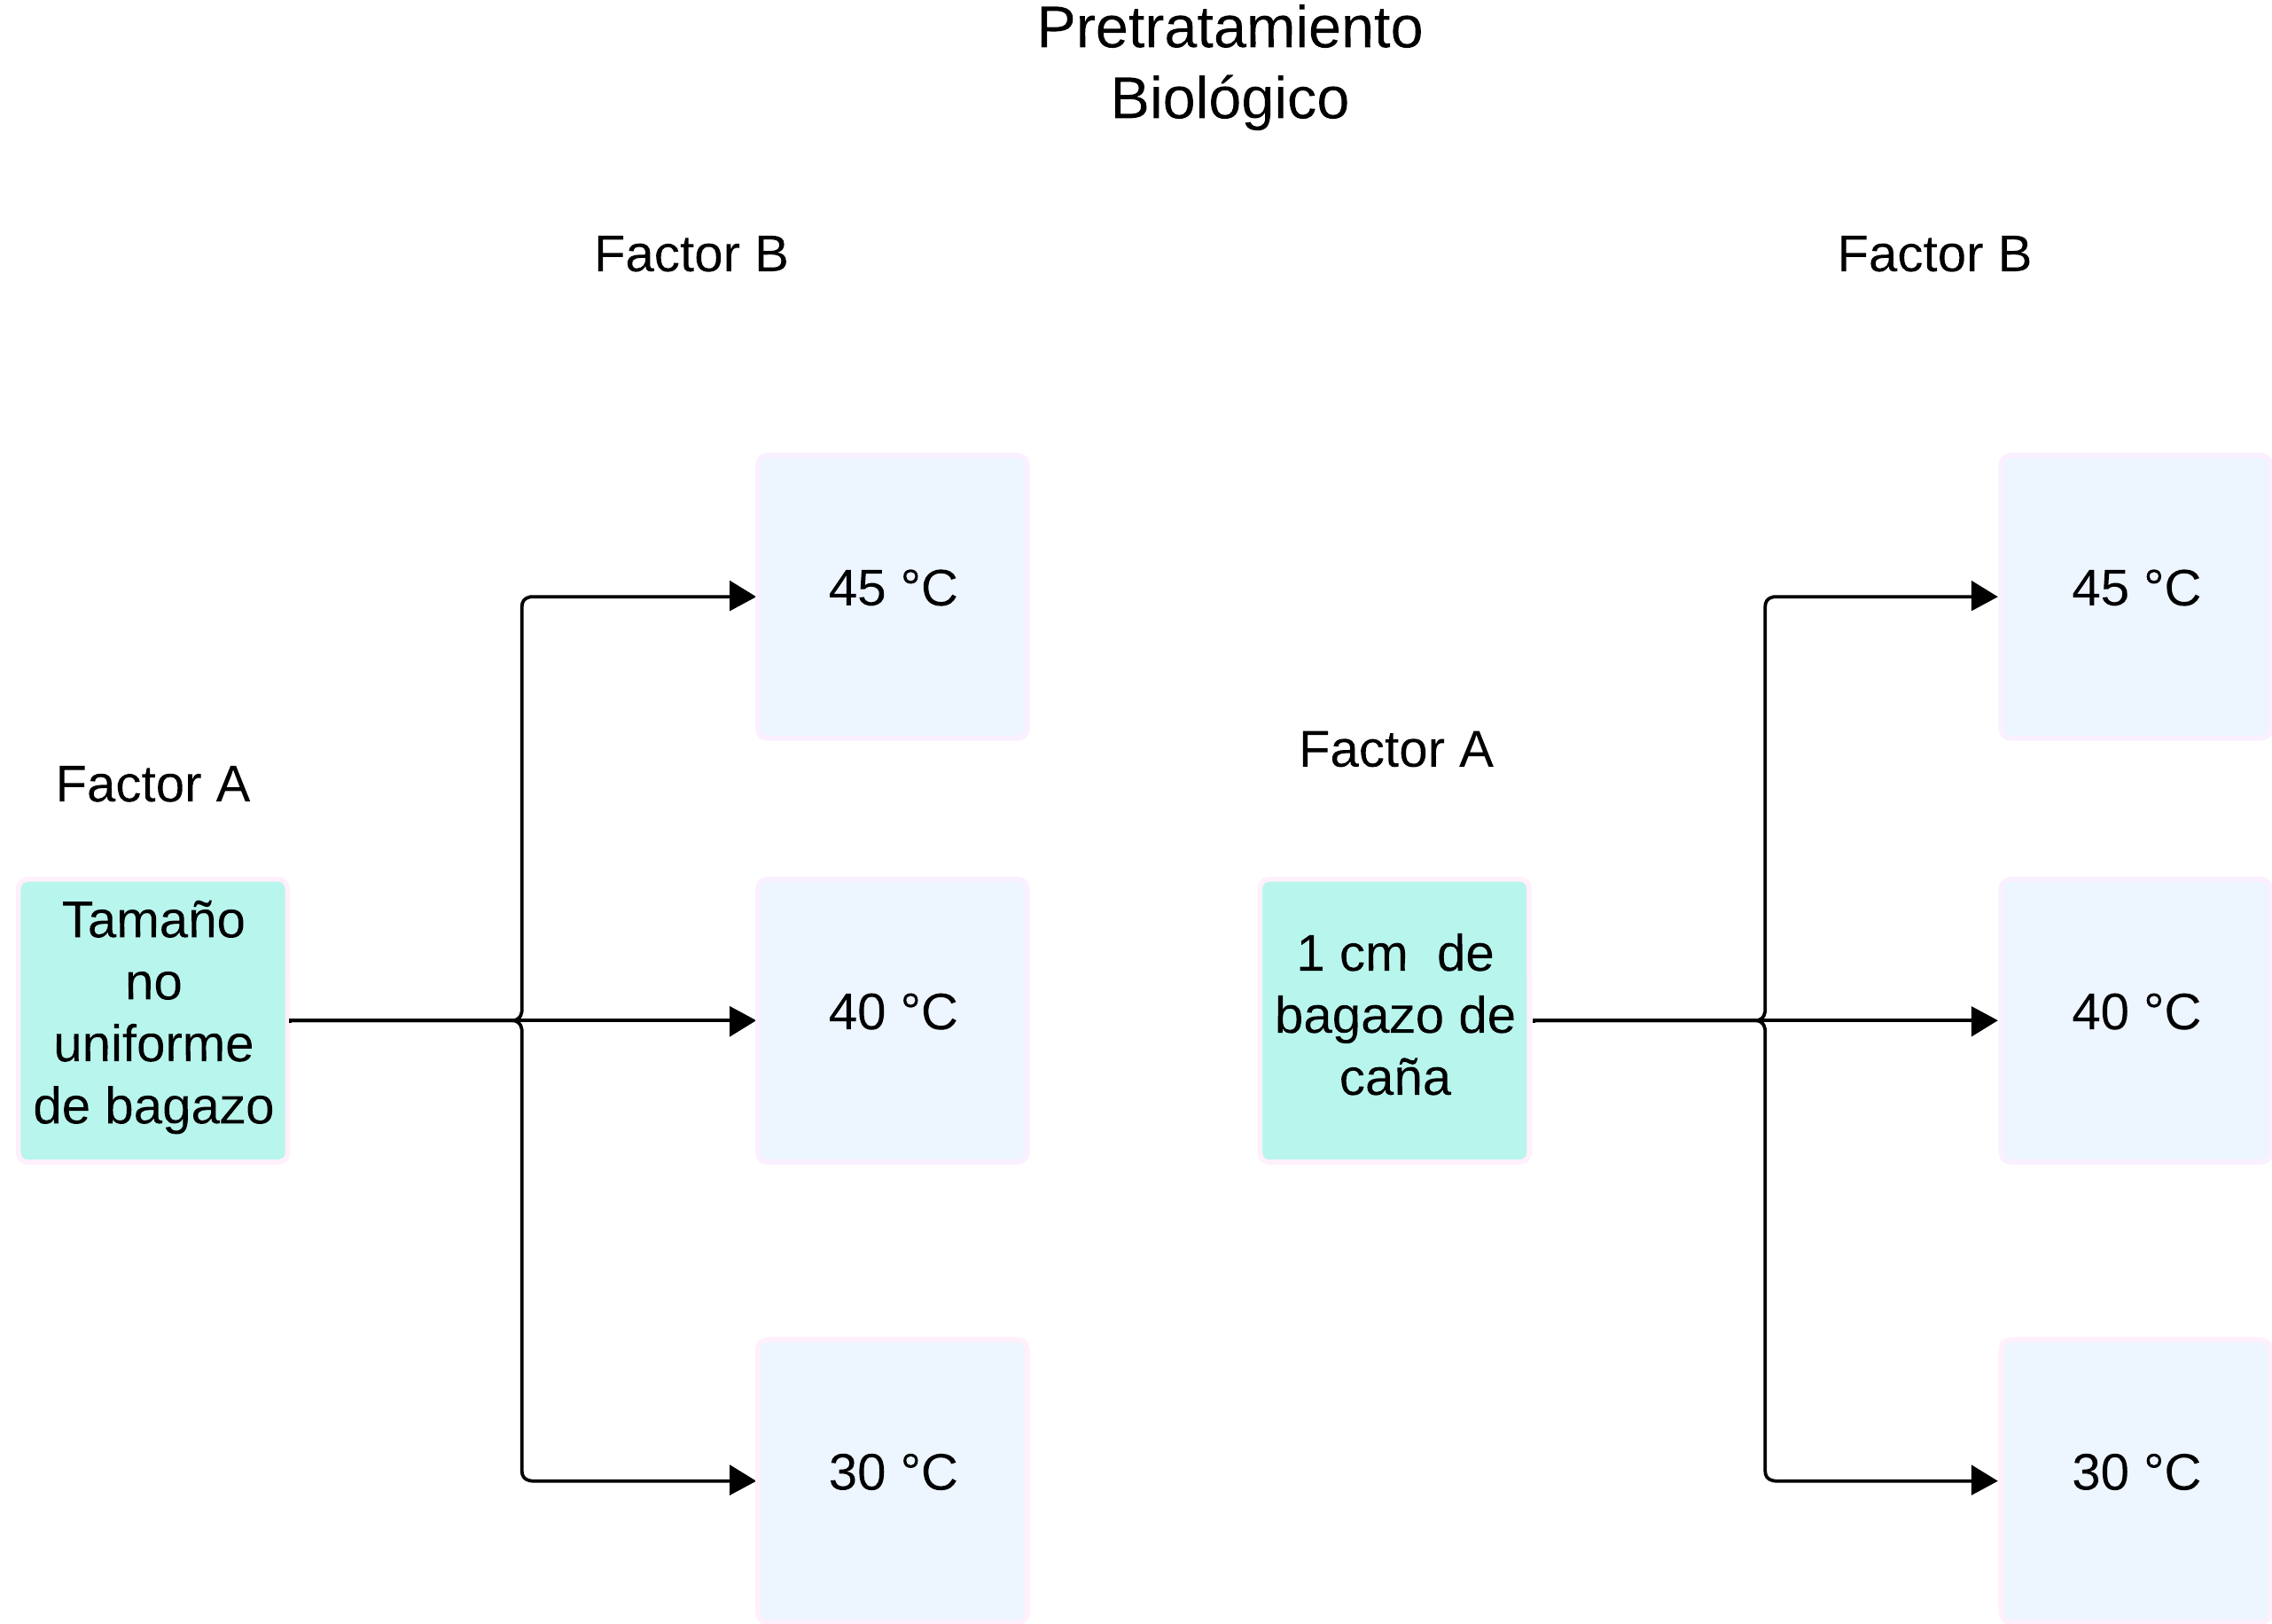
\includegraphics[width=0.7\linewidth]{imagenes/diagramabiologico}
			\caption{Diagrama de los pretratamientos.}
			\label{Diagrama biologico}
		\end{figure}
		
		
	%%%%%%%%%%%%%%%%%%%%%%%%%%%%%%%%%%%%%%%%%%%%%%%%%%%%%%%%%%%%%%%%%%%%%%%%%%%%%%%%%%%%%%%%%%%%%%%%%%%%%%%%%%%%%%%%%%%%%%%%%%%%%%%%%%%%%%%%%%%%%%%%%%%%%%%%%%%%%%%%%%%%%%%%%%%%%%%%%
		
		
		
	
		
	\subsubsection{ Diseño experimental del pretratamiento Alcalino}
	\label{Diseño factorial del pretratamiento alcalino}

Para el caso del pretratamiento alcalino con hidróxido de sodio las temperaturas que se trabajaron fueron 80 °C, 90 °C y 95 °C. También se modificó el tamaño de las partículas de bagazo y el tiempo de producción. En la Tabla \ref{tab:Variablesalcalino} se mencionan las cantidades por insumo que se utilizaron para las pruebas con pretratamiento alcalino. El mezclado del reactivo es importante dado que nos ayuda a mantener la mezcla y la temperatura homogénea dentro del reactor tipo Batch, por lo que también menciona las condiciones de mezclado.


	\begin{table}[H]
	\centering
	\caption{Condiciones de operación fijas del reactor  para el pretratamiento biologico del bagazo de caña.}
	\label{tab:Variablesalcalino}
	\resizebox{\textwidth}{!}{
		\begin{tabular}{| c | c | c | c | c | c |      }
			\hline
			\textbf{Cantidad de} & \textbf{Cantidad de} & \textbf{Volumen de la carga} & \textbf{Tiempo del pretratamiento} & \multicolumn{2}{c|}{ \textbf{Condiciones de agitación} } \\  
			\textbf{bagazo de caña} & \textbf{humus de lombriz} & \textbf{ } & \textbf{Carga de humus} & \multicolumn{2}{c|}{  }  \\  
			\hline
			
			\multirow{5}{*}{4 \% p/v } & \multirow{5}{*}{2\% p/v }  & \multirow{6}{*}{6 l} & \multirow{3}{*}{5400} & \multirow{6}{*}{ 10 s encendido/apagado} & \multirow{6}{*}{142 RPM}  \\ 
			& & & &  &  \\ 
			& & & &  &   \\ 
			\cline{4-4}
			180 g& 300 g &  & \multirow{3}{*}{7870} &  & \\
			& & & & &   \\
			& & & &  &  \\ 
			\hline
		\end{tabular}
	}
\end{table}




De la misma forma, cada pretratamiento fue realizado modificando tres factores. El factor A es el tamaño de partícula, para el cual se consideraron dos niveles: TNUB y 1 cm. El factor B es la temperatura, y para este se consideraron tres niveles: 95 °C , 90 °C, 80 °C. Por último, el factor C que es el tiempo de pretratamiento, tiene dos niveles: 5400 s y 7870 s. En total se realizaron 12 experimentos para el pretratamiento alcalino, como se muestra en la Tabla \ref{alcalino}. 

\begin{table}[H]
	\centering
	\caption{Condiciones de operación del reactor para la producción de bioetanol 2G con pretratamiento biológico. Diseño de experimentos.}
	\label{alcalino}
	\begin{tabular}{|c|c|c|c|}
		\hline
		\textbf{Num de} & \textbf{Temperatura} & \textbf{Tamaño de } & \textbf{Tiempo} \\ 
		\textbf{de experimento}	&\textbf{ (°C)}&\textbf{ bagazo}  &\textbf{(s)}	\\ \hline
		1 & \multirow{4}{*}{95} & \multirow{2}{*}{TNUB*} & 5400   \\ \cline{1-1} \cline{4-4}
		2 &  &  & 7870  \\ \cline{3-4}  \cline{1-1} 
		3 &  & \multirow{2}{*}{1 cm} & 5400  \\  \cline{1-1} \cline{4-4}
		4 &  &  & 7870  \\ \cline{1-1}  \hline
		5 & \multirow{4}{*}{90}& \multirow{2}{*}{TNUB*} & 5400  \\ \cline{1-1}  \cline{4-4}
		6 &  &  & 7870   \\ \cline{1-1} \cline{3-4}
		7 &  & \multirow{2}{*}{1 cm} & 5400  \\ \cline{1-1}\cline{4-4}
		8 &  &  & 7870 \\ \hline
		9 & \multirow{4}{*}{80} & \multirow{2}{*}{TNUB*} & 5400  \\ \cline{1-1}\cline{4-4}
		10 &  &  & 7870   \\ \cline{1-1} \cline{3-4}
		11 &  &\multirow{2}{*}{1 cm} & 5400 \\ \cline{1-1}\cline{4-4}
		12 &  &  & 7870  \\ \hline
	\end{tabular}
		\\[3 pt] % Espacio adicional
	% {\raggedright \footnotesize $^{*}$Tamaño no uniforme de bagazo. \par}
	\footnotesize{$^{*}$  Tamaño no uniforme de bagazo.}
\end{table}



A continuación se presenta un diagrama donde se clasifica por factores cada variable a considerar, esto solo para el caso del pretratamiento alcalino, ver figura  \ref{Diagrama1}.



\begin{figure} [H]
	\centering
	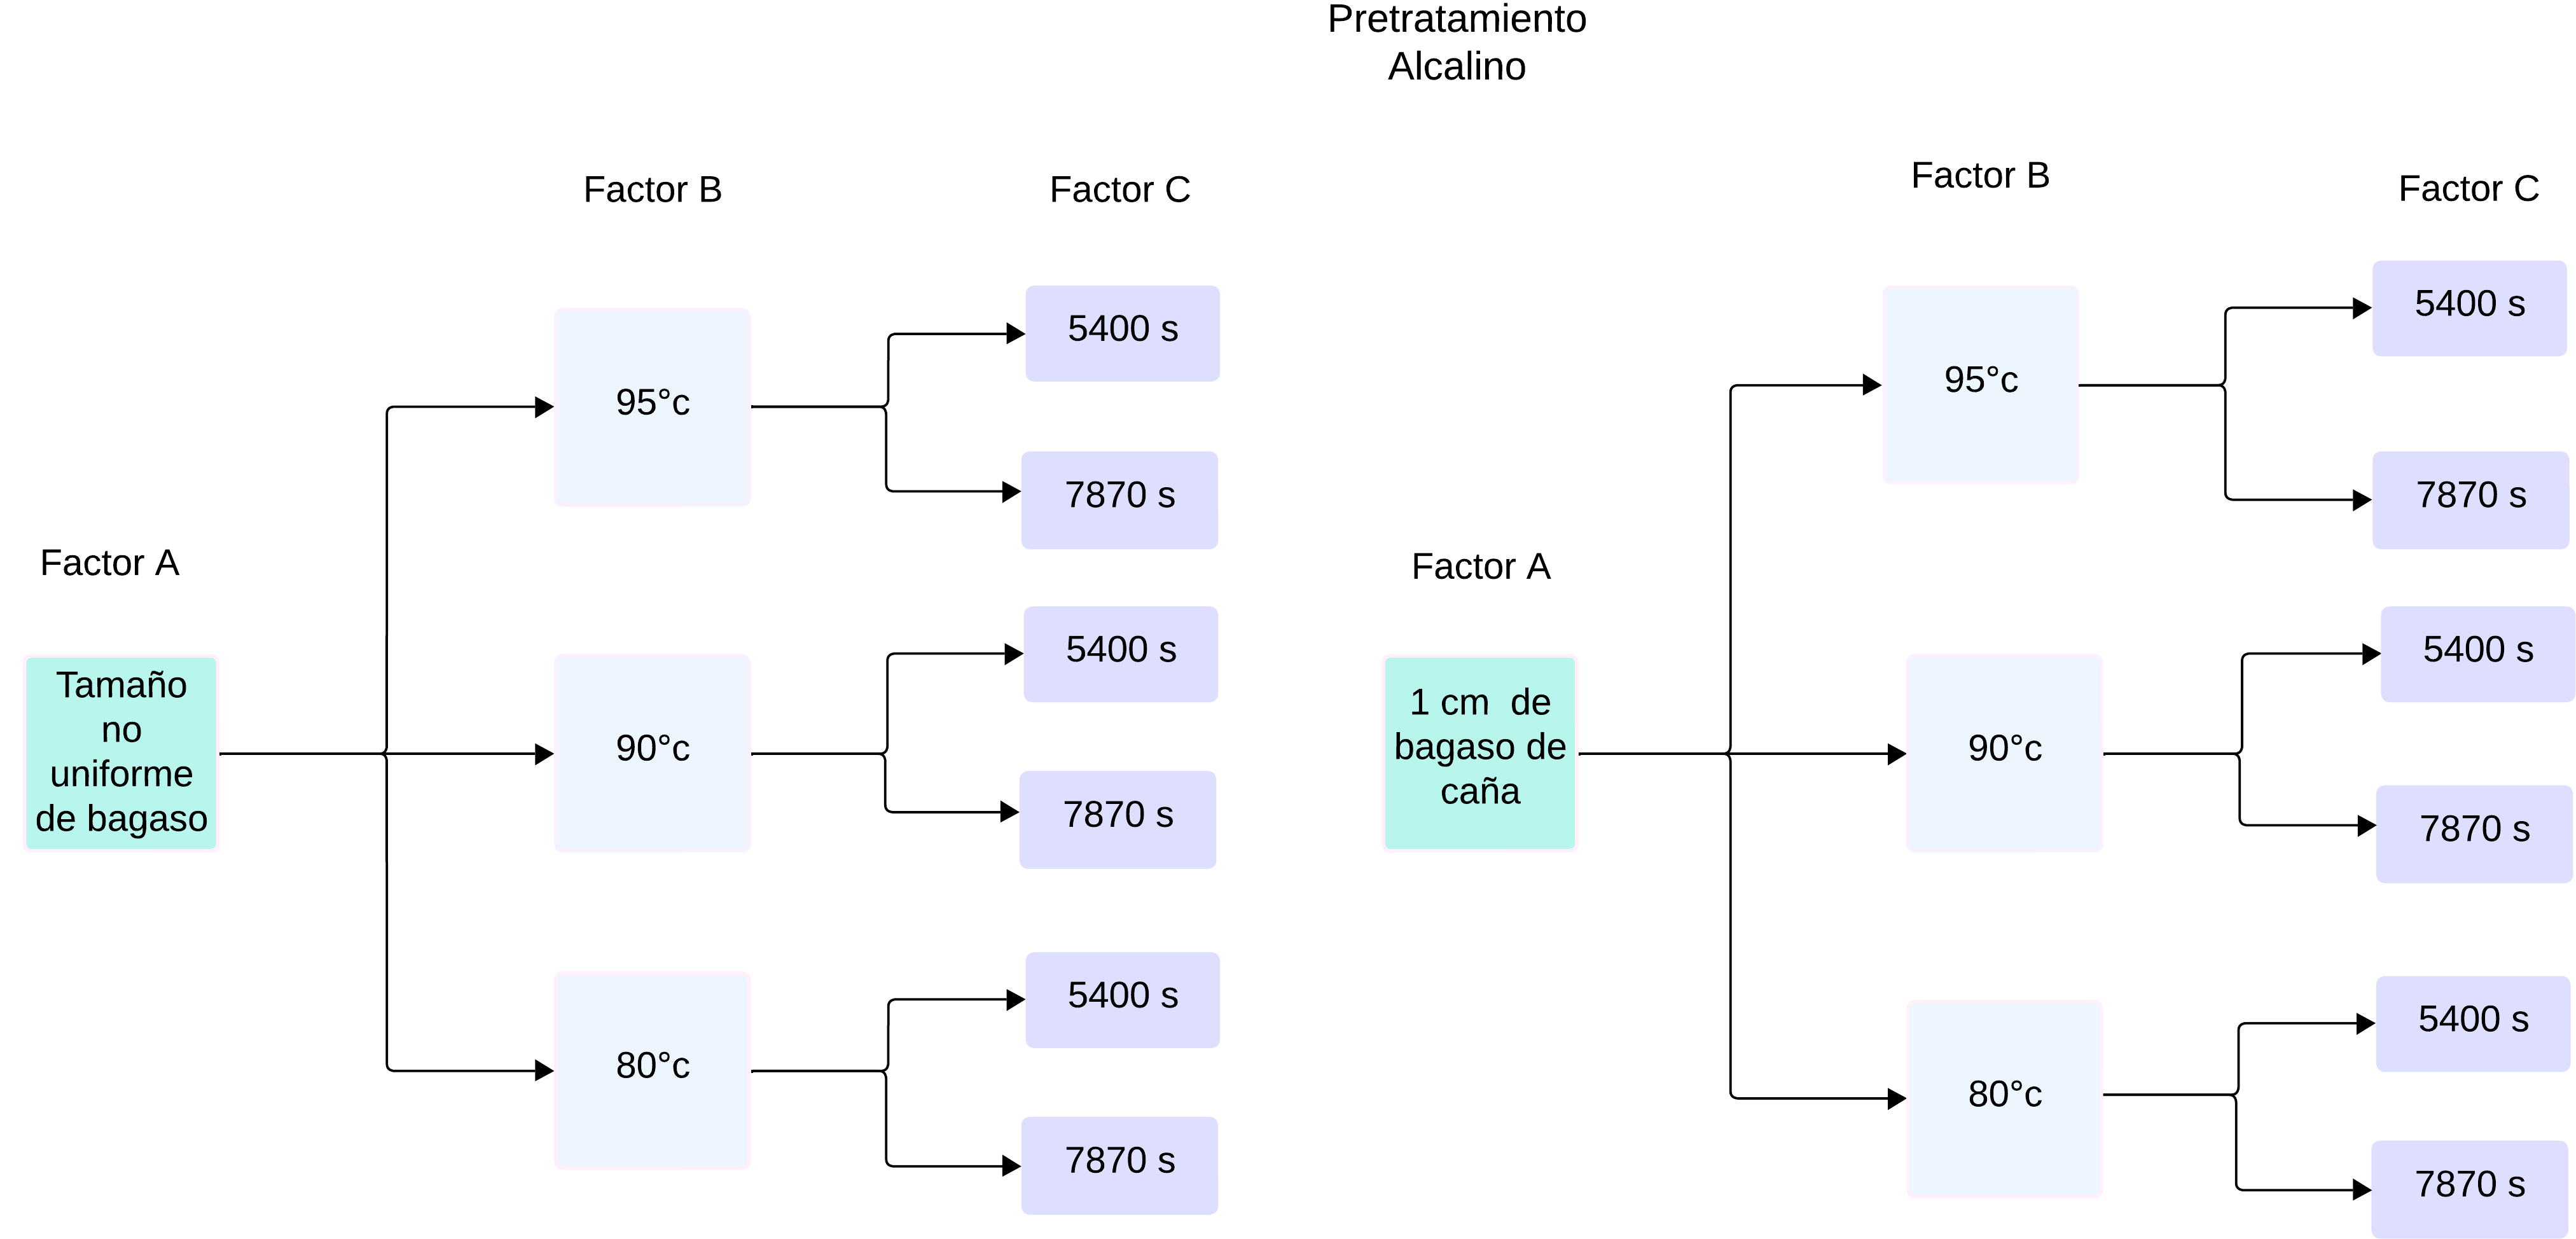
\includegraphics[width=0.9\linewidth]{imagenes/Diagrama alcalino}
	\caption{Diagrama de los pretratamientos.}
	\label{Diagrama1}
\end{figure}



%%%%%%%%%%%%%%%%%%%%%%%%%%%%%%%%%%%%%%%%%%%%%%%%%%%%%%%%%%%%%%%%%%%%%%%%%%%%%%%%%%%%%%%%%%%%%%%%%%%%%%%%%%%%%%%%%%%


%\singlespacing
	
		\subsubsection{Diseño de experimentos para la configuración:
			sacarificación y fermentación simultaneas (SSF)}
		\label{SacariSF}	
		
%		\onehalfspacing
		
		La producción de bioetanol fue realizada usando la configuración de hidrólisis y fermentación simultáneas. Las condiciones de operación corresponden al diseño del proceso presentado en la tesis de \cite{Arturo2022evaluacion}. Se debe precisar la carga de biomasa, que es la cantidad de bagazo previamente pretratado con alguno de los dos métodos considerados, la levadura necesaria para una buena fermentación, el pH de la solución dentro del reactor, la carga enzimática que es un elemento clave  para llevar  cabo la hidrólisis, y por ultimo la temperatura de la SSF. En la Tabla \ref{tab:Variables a modificar para la hidrolisis y fermentacion}, se muestran los valores de cada uno de los elementos a tomar en cuenta para la implementar el proceso SSF. \\[0.5em]
		
		\begin{table} [h!]
			\centering
			\caption{Variables a modificar en la SSF}
			\label{tab:Variables a modificar para la hidrolisis y fermentacion}
			\small
			\resizebox{17cm}{!} {
			\begin{tabular}{|c|c|c|c|c|c|c|c|c|}
				\hline
			\textbf{Biomasa}  &\textbf{ Volumen}  & \textbf{Carga de } & \textbf{Carga}  & \textbf{Inoculo}  &\textbf{ Ph}  & \textbf{Temperatura } & \textbf{Tiempo}   \\
				 &   & \textbf{ biomasa}  & \textbf{enzimática } & \textbf{de levadura } & &  &     \\
				
				\hline
			\multirow{2}{*}{Bagazo de caña} &\multirow{2}{*}{2 l}  &\multirow{2}{*}{5\%}  & \multirow{2}{*}{20 UPF/g } & \multirow{2}{*}{10\% } &\multirow{2}{*}{ 5} & \multirow{2}{*}{43 °C} & \multirow{2}{*}{48h }   \\
			  &   & & &  &  & &     \\		
				\hline
			\end{tabular}}
		\end{table}
		

		
			\begin{itemize}
			\item  Carga enzimática
	     	\end{itemize}
		
		
	La carga enzimática se refiere a  la cantidad de enzimas que se introduce durante el proceso SSF y está dada en unidades de papel filtro por gramo de sustrato (UPF/g). UPF es una medida de laboratorio para expresar la actividad enzimática. La ecuación \ref{carga} permite calcular la carga enzimática en unidades de ml, en función de la cantidad de unidades de papel filtro (UPF),  \cite{Arturo2022evaluacion}).
			
	\begin{equation}
		\label{carga}
		\text{carga enzimática (ml)} = \frac{3.7}{UPF}
	\end{equation}
	

	
		

	%%%%%%%%%%%%%%%%%%%%%%%%%%%%%%%%%%%%%%%%%%%%%%%%%%%%%%%%%%%%%%%%%%%%%%%%%%%%%%%%%%%%%%%%%%%%%%%%%%%%%%%%%%%%%%%%%%%%%%%%%%%%%%%%%%%%%%%%%%%%%%%%%%%%
			
			
	
			\subsection{Implementación}

			En esta sección se describen las pruebas experimentales, indicando en primera instancia los materiales necesarios en cada pretratamiento, y posteriormente, se mencionan los pasos que conlleva realizar cada prueba.
			

			\subsubsection{Pre-Pretratamiento}

			
			El pre-pretratamiento es un preprocesamiento de la biomasa para someterla posteriormente al pretratamiento del tipo seleccionado para activar la producción de azúcares fermentables. El pre-pretratamiento incluye clasificar el tamaño de bagazo por tamizado, y secarlo en caso de tener humedad. El material y compuestos para poder clasificar y limpiar el bagazo son los siguientes
			\\[0.5em]
			\textbf{Compuestos} 
			\begin{itemize}[label=\textcolor{blue}{$\bullet$}]
			 \item	\textit{ Bagazo de caña }
			\end{itemize} 
			
			
			\textbf{Materiales} \\[0.5em]
			
			
			\begin{tabular}{p{0.3\textwidth}p{0.3\textwidth}p{0.3\textwidth}}
			\textit{	$\bullet$ Lona} &  \textit{$\bullet$  Malla cuadrada 1 cm} & \textit{$\bullet$ Bolsa plástica  }\\
				&&\textit{de 30×40 cm} \\
				\textit{$\bullet$ Báscula} & \textit{$\bullet$ Cubeta con capacidad de 10 l} & 
			\end{tabular}
		\\[0.5em]
			
			
			\textbf{Procedimiento}
			\\[0.5em]
			\textbf{1.} Se implementó una barrera de protección usando una lona impermeable extendida sobre el piso, evitando el contacto directo del bagazo de caña con superficies contaminantes. Sobre esta superficie aislante, se distribuyó uniformemente el bagazo de caña para facilitar el secado pasivo y la eliminación controlada de su humedad residual. El proceso se muestra en la Figura~\ref{secado1}

			
			\textbf{2.}	La clasificación por tamaño se efectuó usando un arreglo de dos mallas metálicas de 1 cm, montadas en serie sobre un recipiente de 10 L. Mediante agitación rítmica del bagazo colocado en la malla superior (Figura \ref{cernir_bagazo_B}), las fracciones menores a 1 cm fueron seleccionadas por gravedad hacia la cubeta, mientras que las partículas mayores se retuvieron en el tamiz.
		
			
				\begin{figure}[H]
				\centering
				\begin{minipage}{0.46\textwidth}
					\centering
					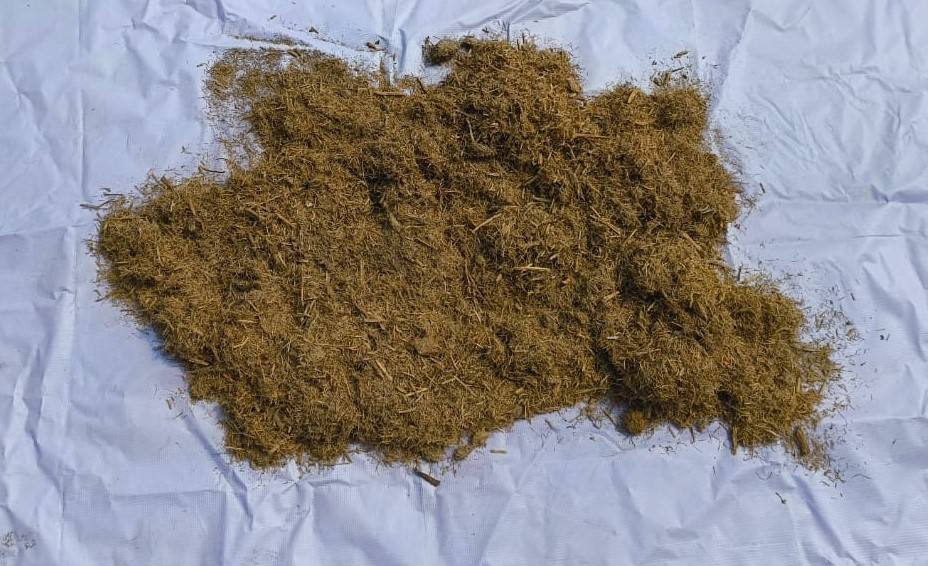
\includegraphics[width=5cm, height=3cm]{imagenes/secado de bagazo} % Cambia "imagen1.jpg" por el nombre de tu archivo
					\caption{Bagazo de caña tendido sobre una lona.}
					\label{secado1}
				\end{minipage}
				\hfill
				\begin{minipage}{0.48\textwidth}
					\centering
					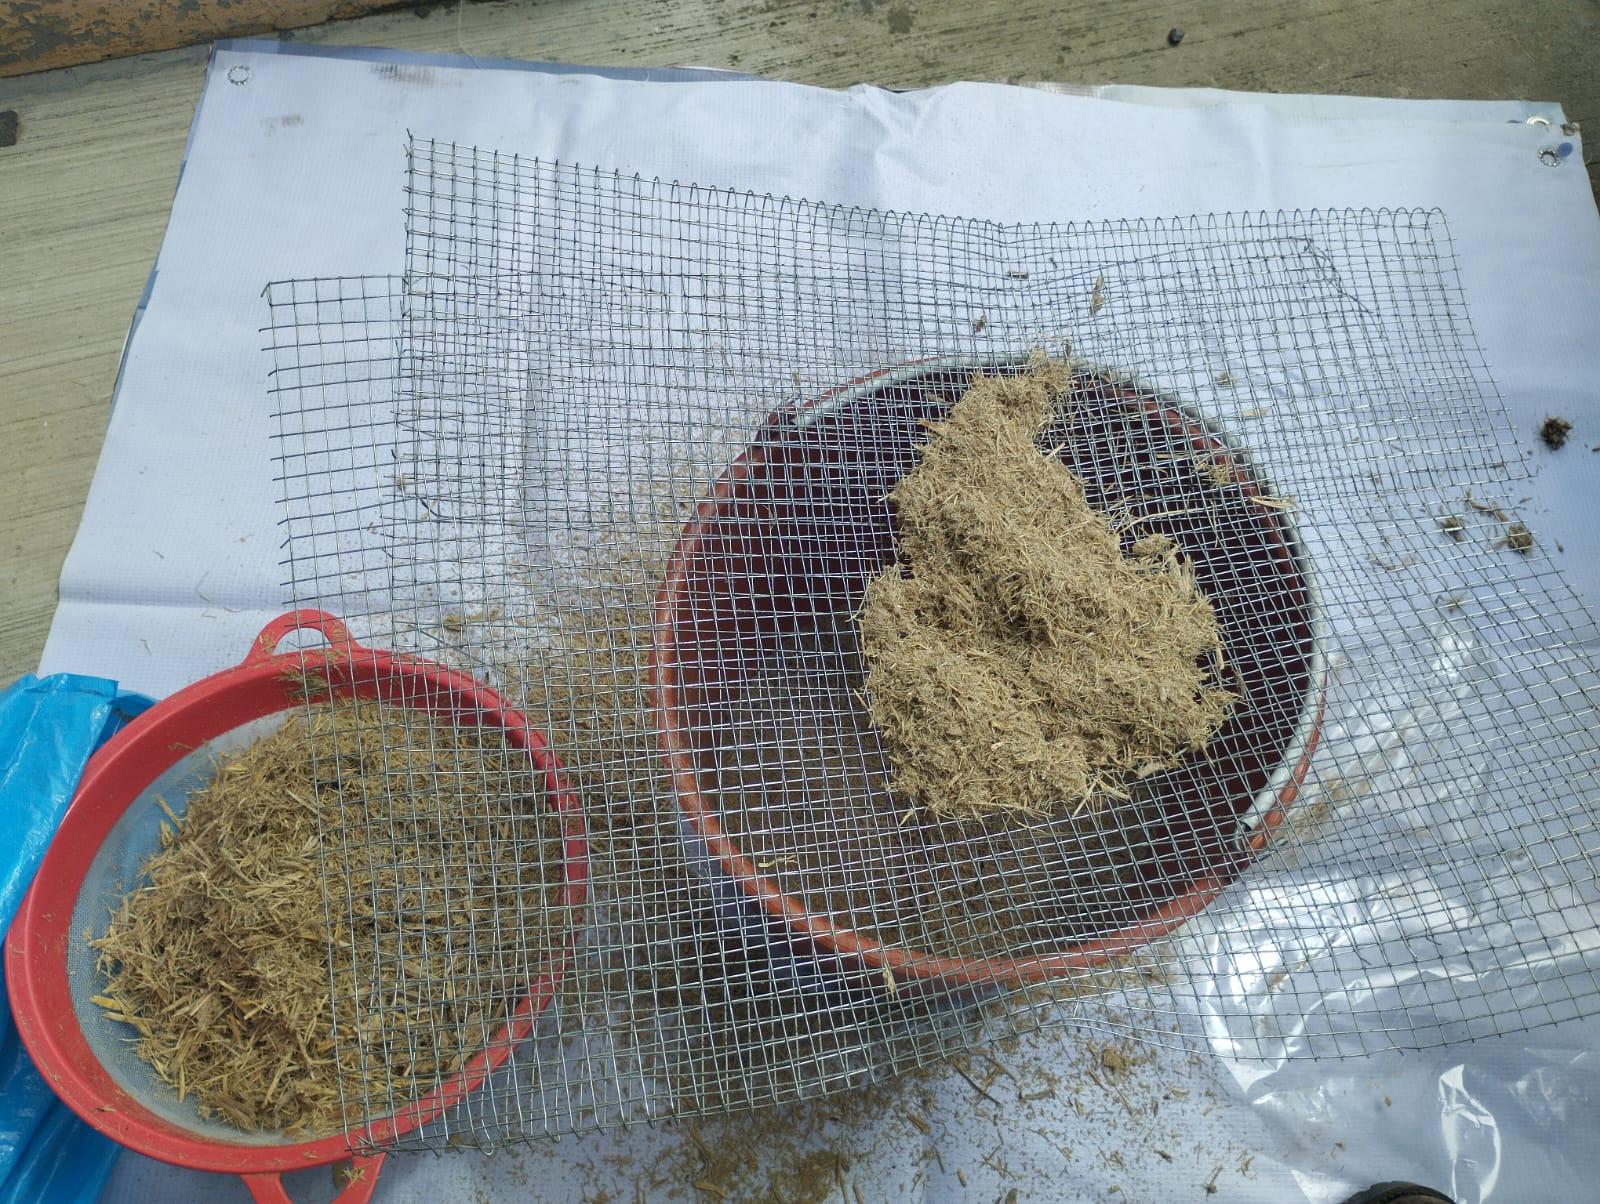
\includegraphics[width=5cm, height=3cm]{imagenes/cernir_bagazo_1} % Cambia "imagen2.jpg" por el nombre de tu archivo
					\caption{El bagazo es cernido con ayuda de la malla de 1 cm.}
					\label{cernir_bagazo_B}
				\end{minipage}
			\end{figure}
			
			
			
			
			
			\textbf{3.}	El bagazo se sometió a dos ciclos adicionales de cribado utilizando el mismo sistema de doble malla (abertura de 1 cm), aplicando un movimiento armónico controlado en cada repetición (Figura \ref{cernir_bagazo_2C}). Este proceso iterativo permitió obtener una fracción de partículas con tamaño significativamente reducido, optimizando la homogeneidad del material resultante.
			
			
			\textbf{4.} Para garantizar un tamaño de partícula uniforme, el bagazo de caña se sometió a un cribado adicional mediante un cedazo de malla más fina, con el objetivo de obtener un material final con una granulometría controlada de 1 cm, lo que optimiza su posterior aprovechamiento en procesos industriales. Ver Figura \ref{cernir_bagazo_cedazo}.
		
		
			\begin{figure}[H]
			\centering
			\begin{minipage}{0.46\textwidth}
				\centering
			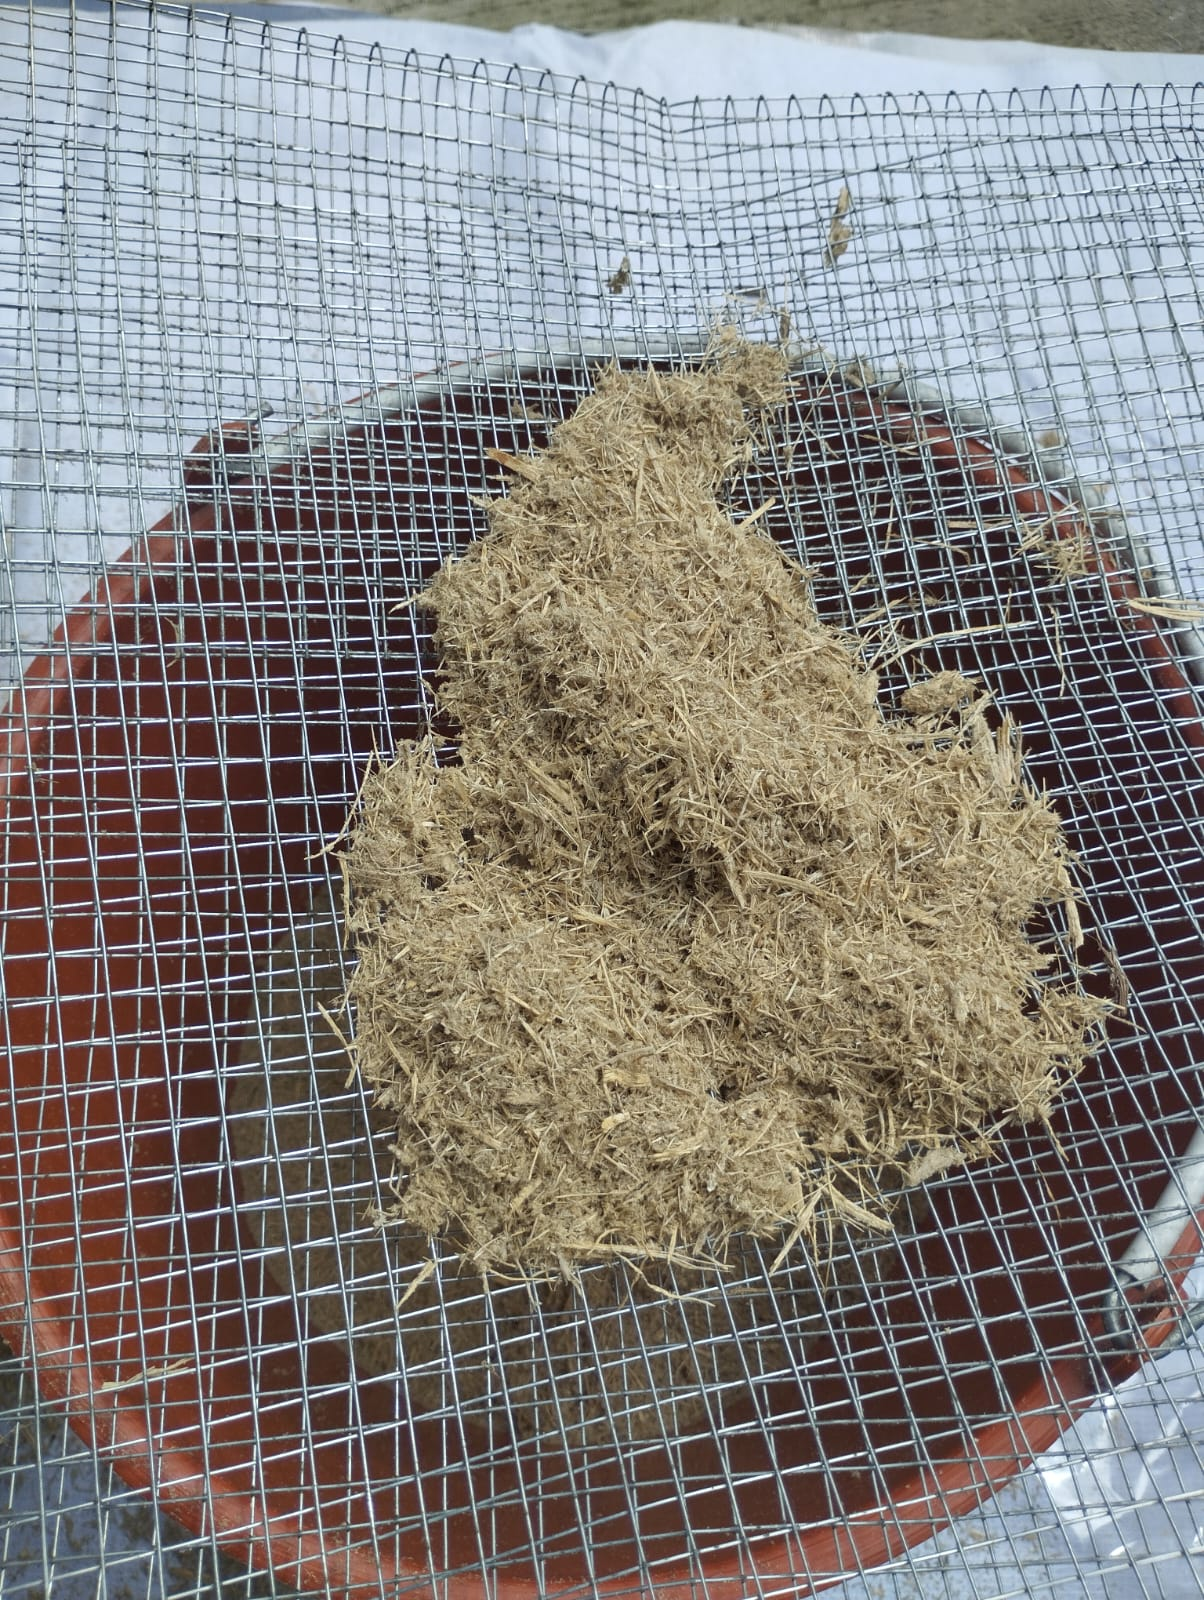
\includegraphics[width=\linewidth, height=4cm, keepaspectratio]{imagenes/cernir_bagazo_2}
			\caption{Momento donde el bagazo es clasificado.}
			\label{cernir_bagazo_2C}
			\end{minipage}
			\hfill
			\begin{minipage}{0.48\textwidth}
				\centering
				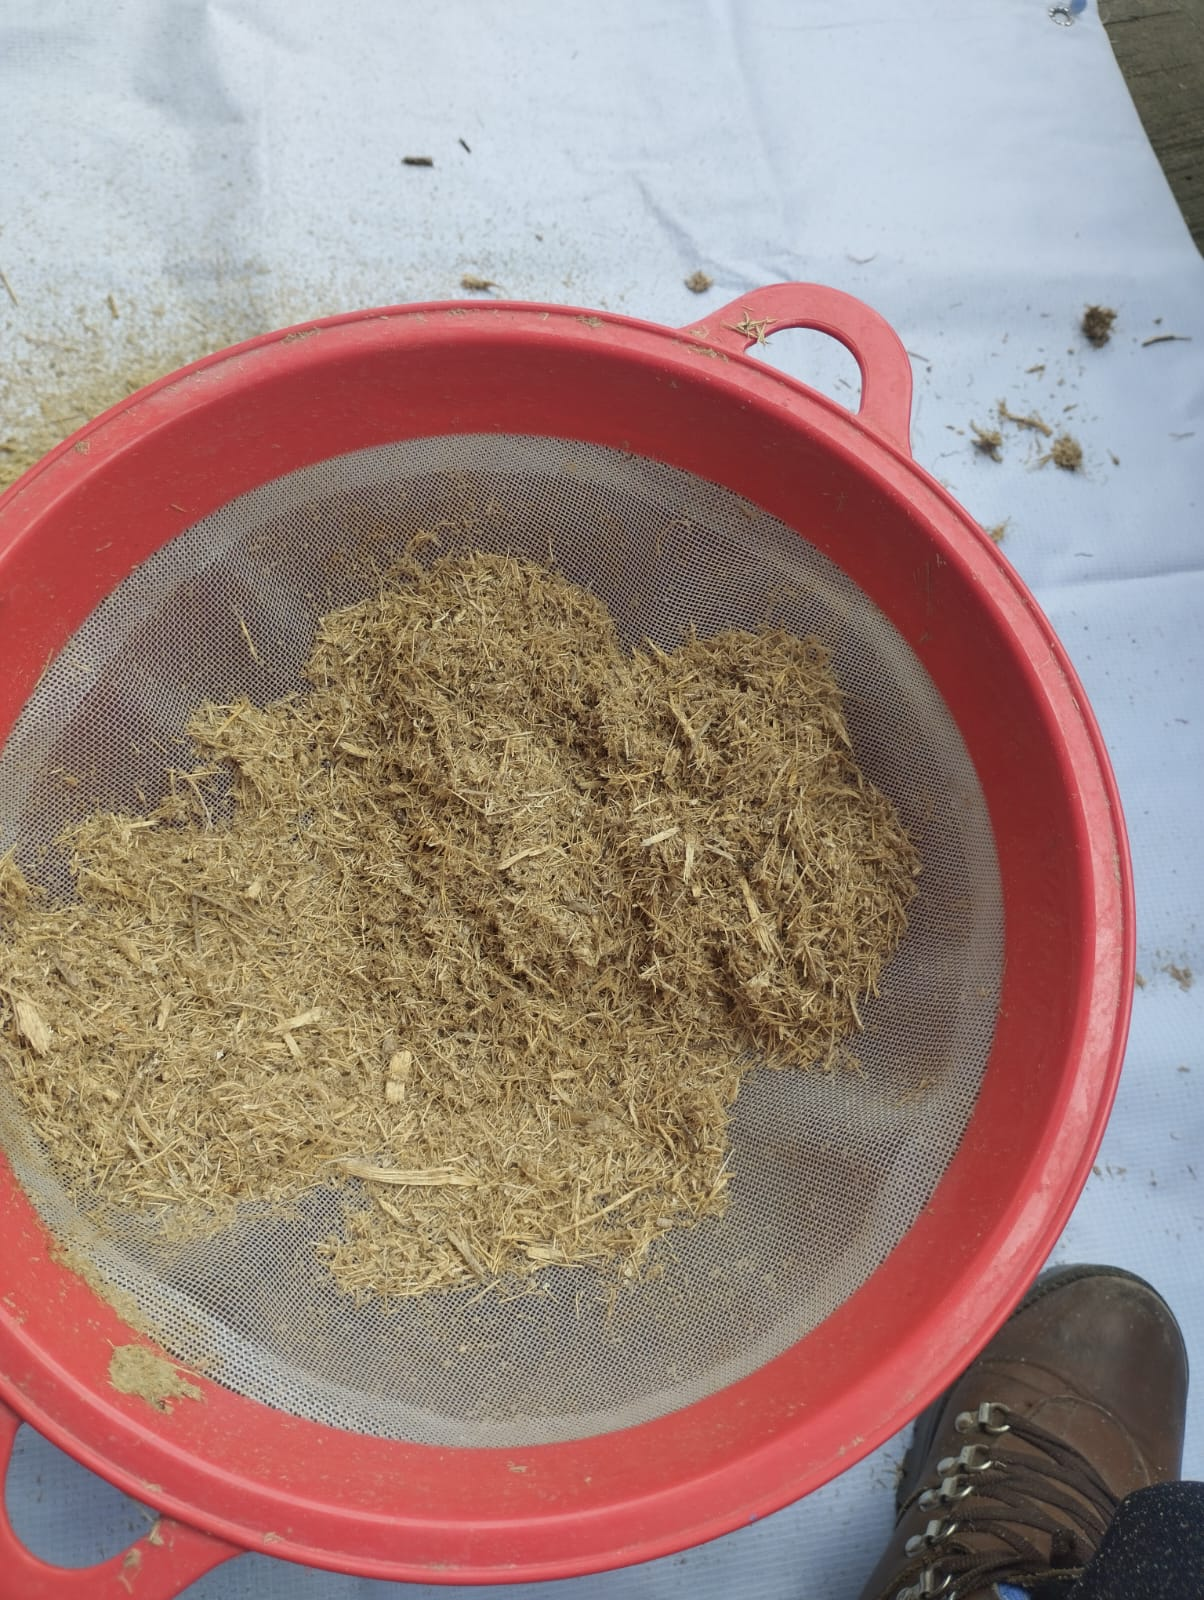
\includegraphics[width=\linewidth, height=4cm, keepaspectratio]{imagenes/cernir_bagazo_cedazo}
				\caption{Clasificación con colador para trozos grandes.}
				\label{cernir_bagazo_cedazo}
			\end{minipage}
		\end{figure}
		
	
			\textbf{5.} El bagazo cernido fue pesado en una báscula hasta alcanzar la masa requerida (240 g o 180 g, según el pretratamiento asignado) y posteriormente se introdujo en una bolsa de plástico, la cual fue sellada herméticamente para evitar alteraciones en su contenido de humedad durante el almacenamiento o transporte.
			
			
			\begin{figure} [H]
				\centering
				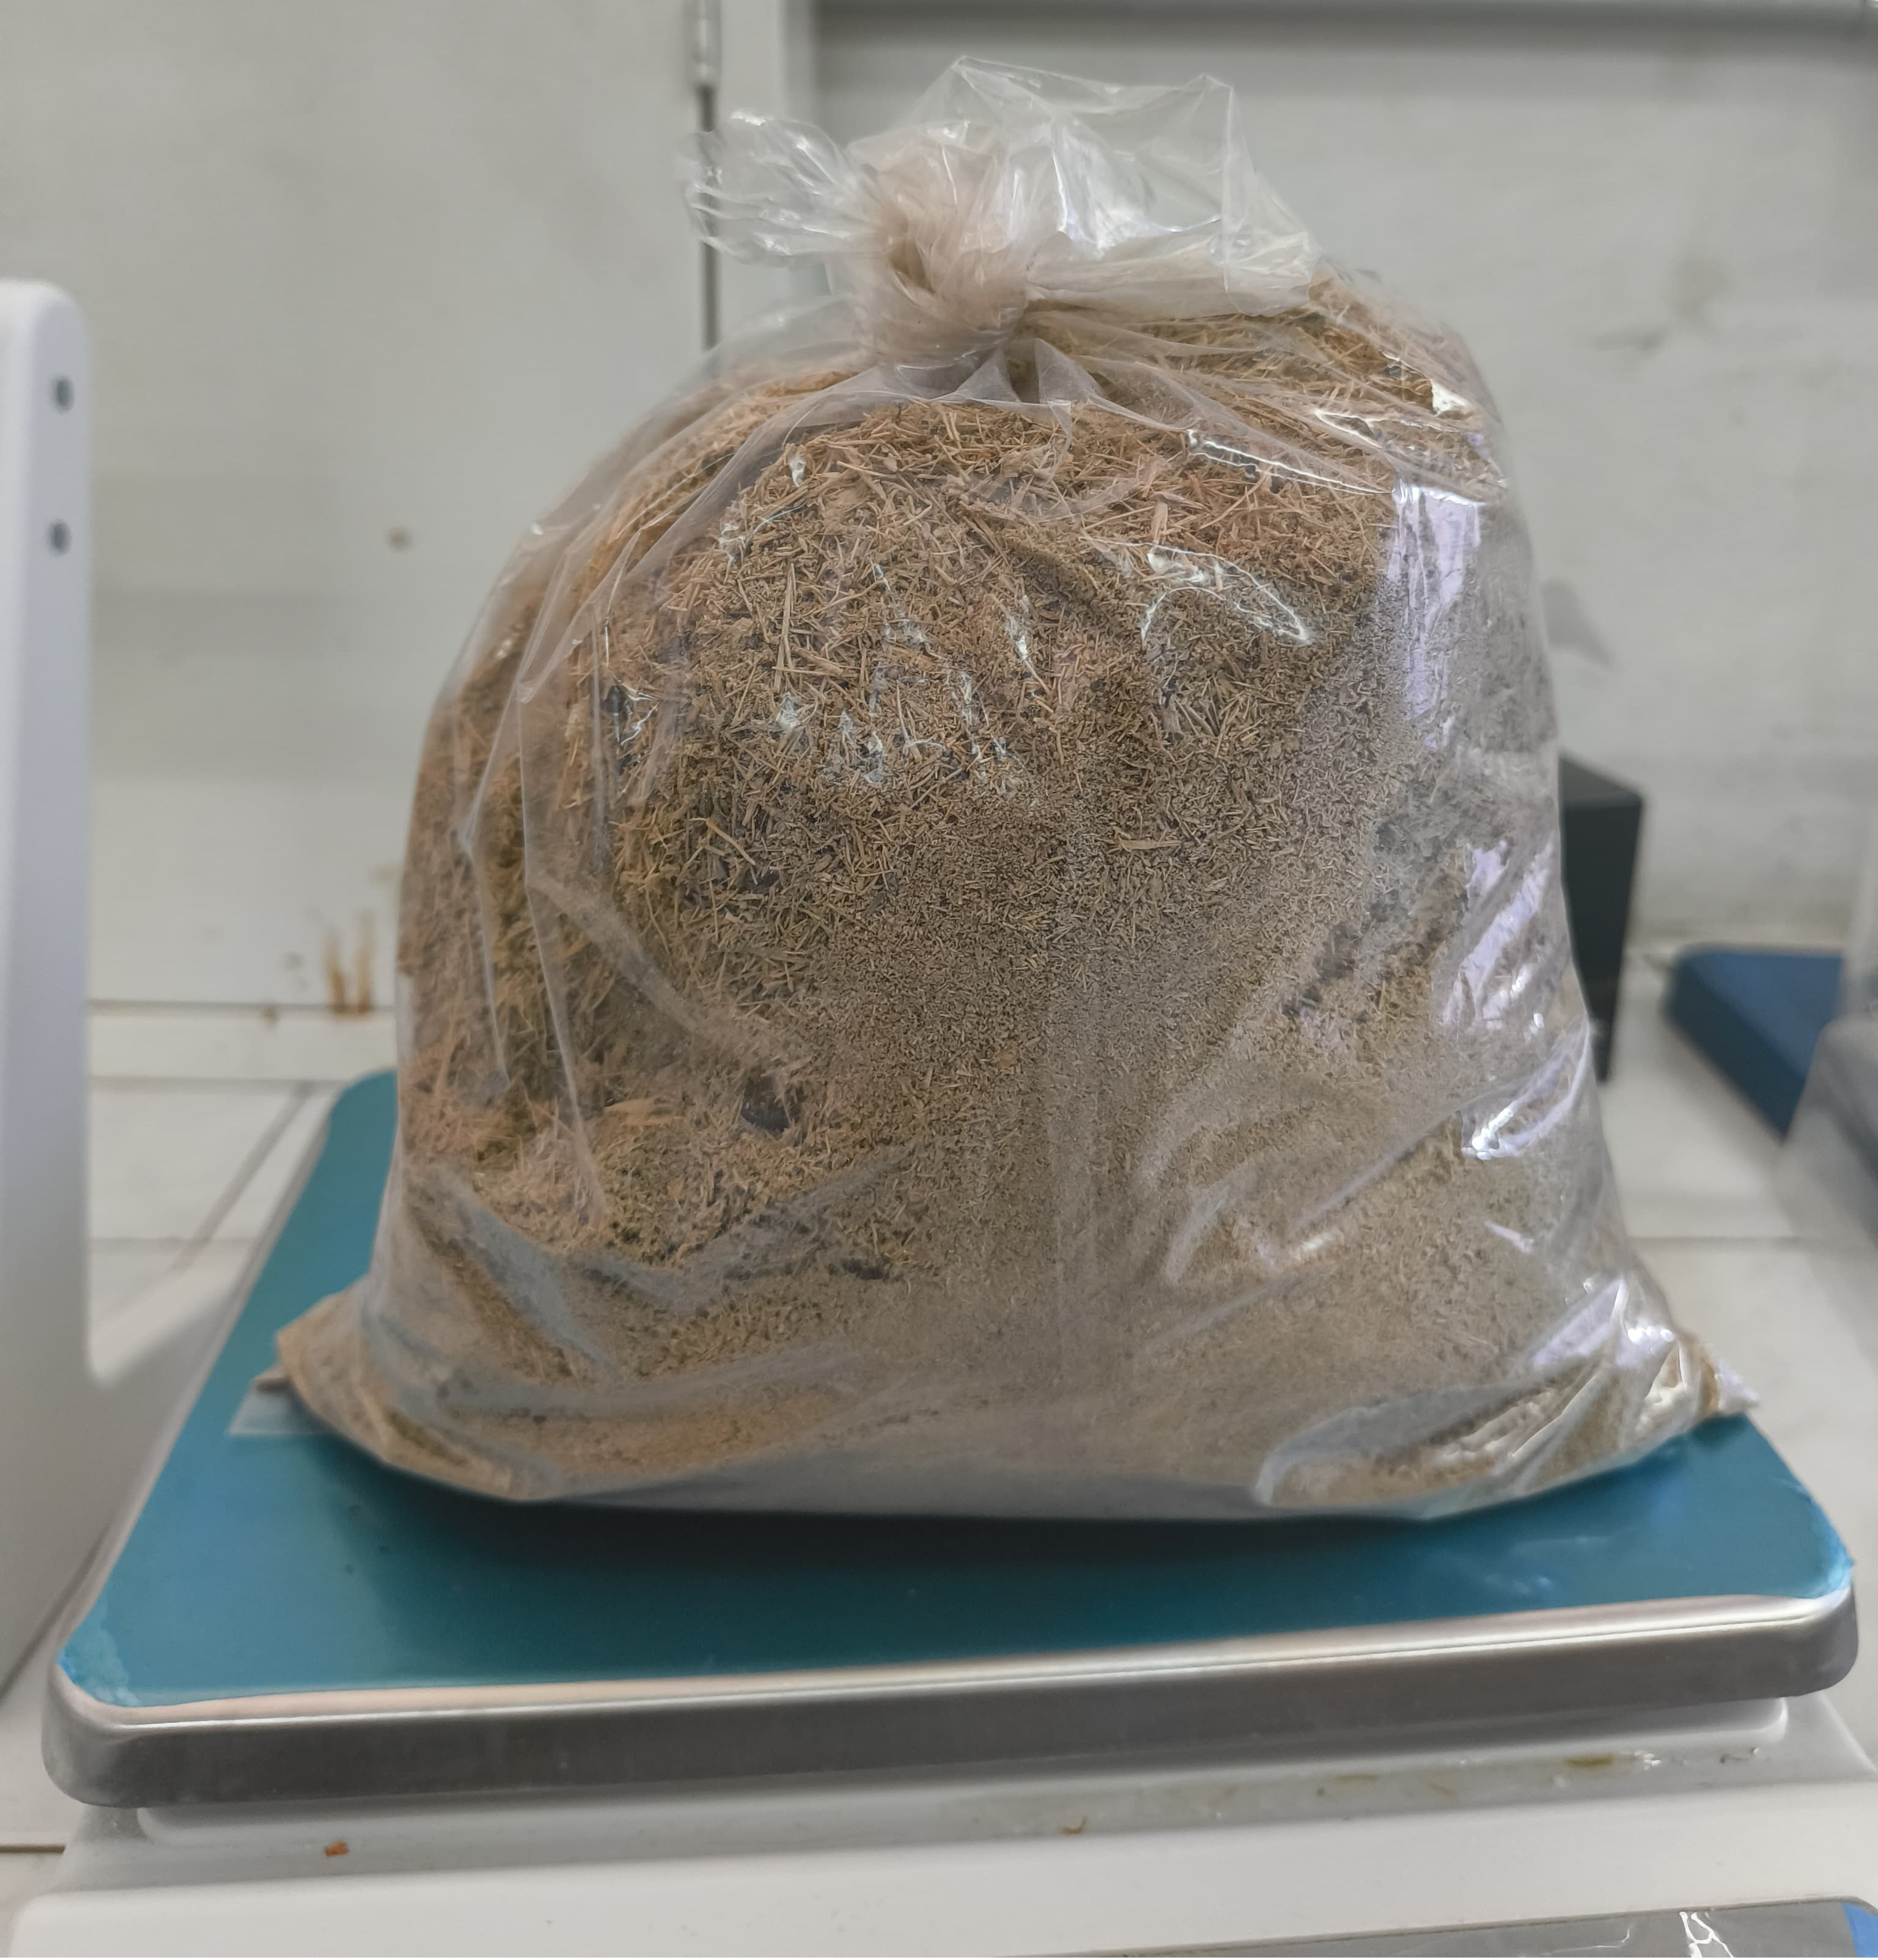
\includegraphics[width=5cm, height=3cm]{imagenes/cernir_bagazo_pesado}
				\caption{El bagazo cernido es colocado en la bolsa y se pesado en una bascula.}
				\label{cernir_bagazo_pesado}
			\end{figure}
			
			
			%%%%%%%%%%%%%%%%%%%%%%%%%%%%%%%%%%%%%%%%%%%%%%%%%%%%%%%%%%%%%%%%%%%%%%%%%%%%%%%%%%%%%%%%%%%%%%%%%%%%%%%%%%%%%%%%%%%%%%%%%%%%%%%%%%%%%%%%%%%%%%%%%%%%%%%%%%%%%%%%
			
			
			\subsubsection{Pretratamiento Biológico}
	
			
		Para la ejecución del pretratamiento biológico se requiirió el siguiente conjunto de materiales y reactivos estandarizados. Posteriormente se mencionan los pasos para la experimentación.\\
			
			\textbf{Compuestos} \\[0.5em]
			

				\begin{tabular}{p{0.3\textwidth}p{0.3\textwidth}}
				\textcolor{blue}{$\bullet$} \textit{Humus de Lombriz}  &	\textcolor{blue}{$\bullet$} \textit{Bagazo de caña}
			\end{tabular} \\[0.5em]
			
			\textbf{Materiales} \\[0.5em] 
	
			\begin{tabular}{p{0.3\textwidth}p{0.3\textwidth}p{0.3\textwidth}}
				$\bullet$ \textit{Agua desmineralizada } & $\bullet$ \textit{Algodón} & $\bullet$ \textit{Bolsa plástica de 30×40 cm }\\
				$\bullet$ \textit{Báscula} & $\bullet$ \textit{Cinta aislante} & $\bullet$ \textit{Cinta de teflón}
			\end{tabular}
			\\[1em]
			
			
			\textbf{Procedimiento}
			\\[0.5em]
			\textbf{1.}	La dosificación del bagazo fue realizada mediante pesaje con una báscula digital utilizando una bolsa plástica de 3 kg como recipiente, hasta alcanzar los 180 g requeridos. Este procedimiento se aplicó únicamente cuando no se empleó la medida estándar de 1 cm de longitud de partícula, en cuyo caso se utilizó directamente el material previamente clasificado y calibrado. Ver Figura \ref{bagazo_variostamaños}.
		
			
			\textbf{2.}	Mediante báscula digital (±0.2 g) y material de vidrio calibrado (vaso de precipitado de 500 mL) se pesó exactamente 350 g de humus de lombriz grado técnico, siguiendo el procedimiento ilustrado en la Figura \ref{humus}.
			
			
				\begin{figure}[H]
				\centering
				\begin{minipage}{0.46\textwidth}
						\centering
					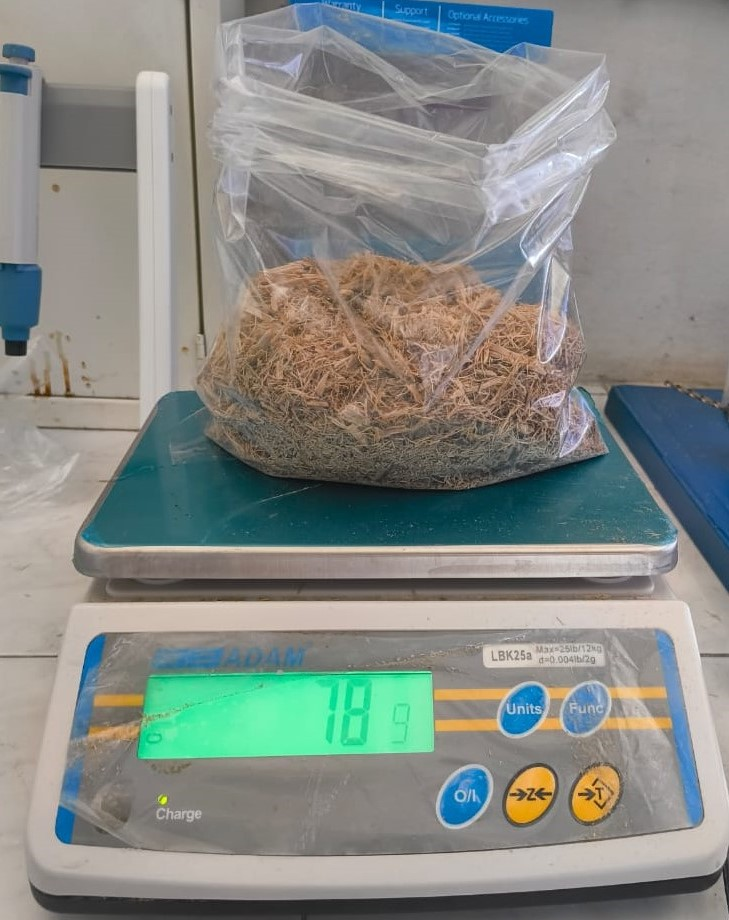
\includegraphics[width=3cm, height=5cm]{imagenes/pesado2}
					\caption{Medición de masa del bagazo de caña, clasificado por tamaño de partícula (1 mm a 10 cm), previo al proceso de bioetanol.}
					\label{bagazo_variostamaños}
				\end{minipage}
				\hfill
				\begin{minipage}{0.48\textwidth}
				\centering
				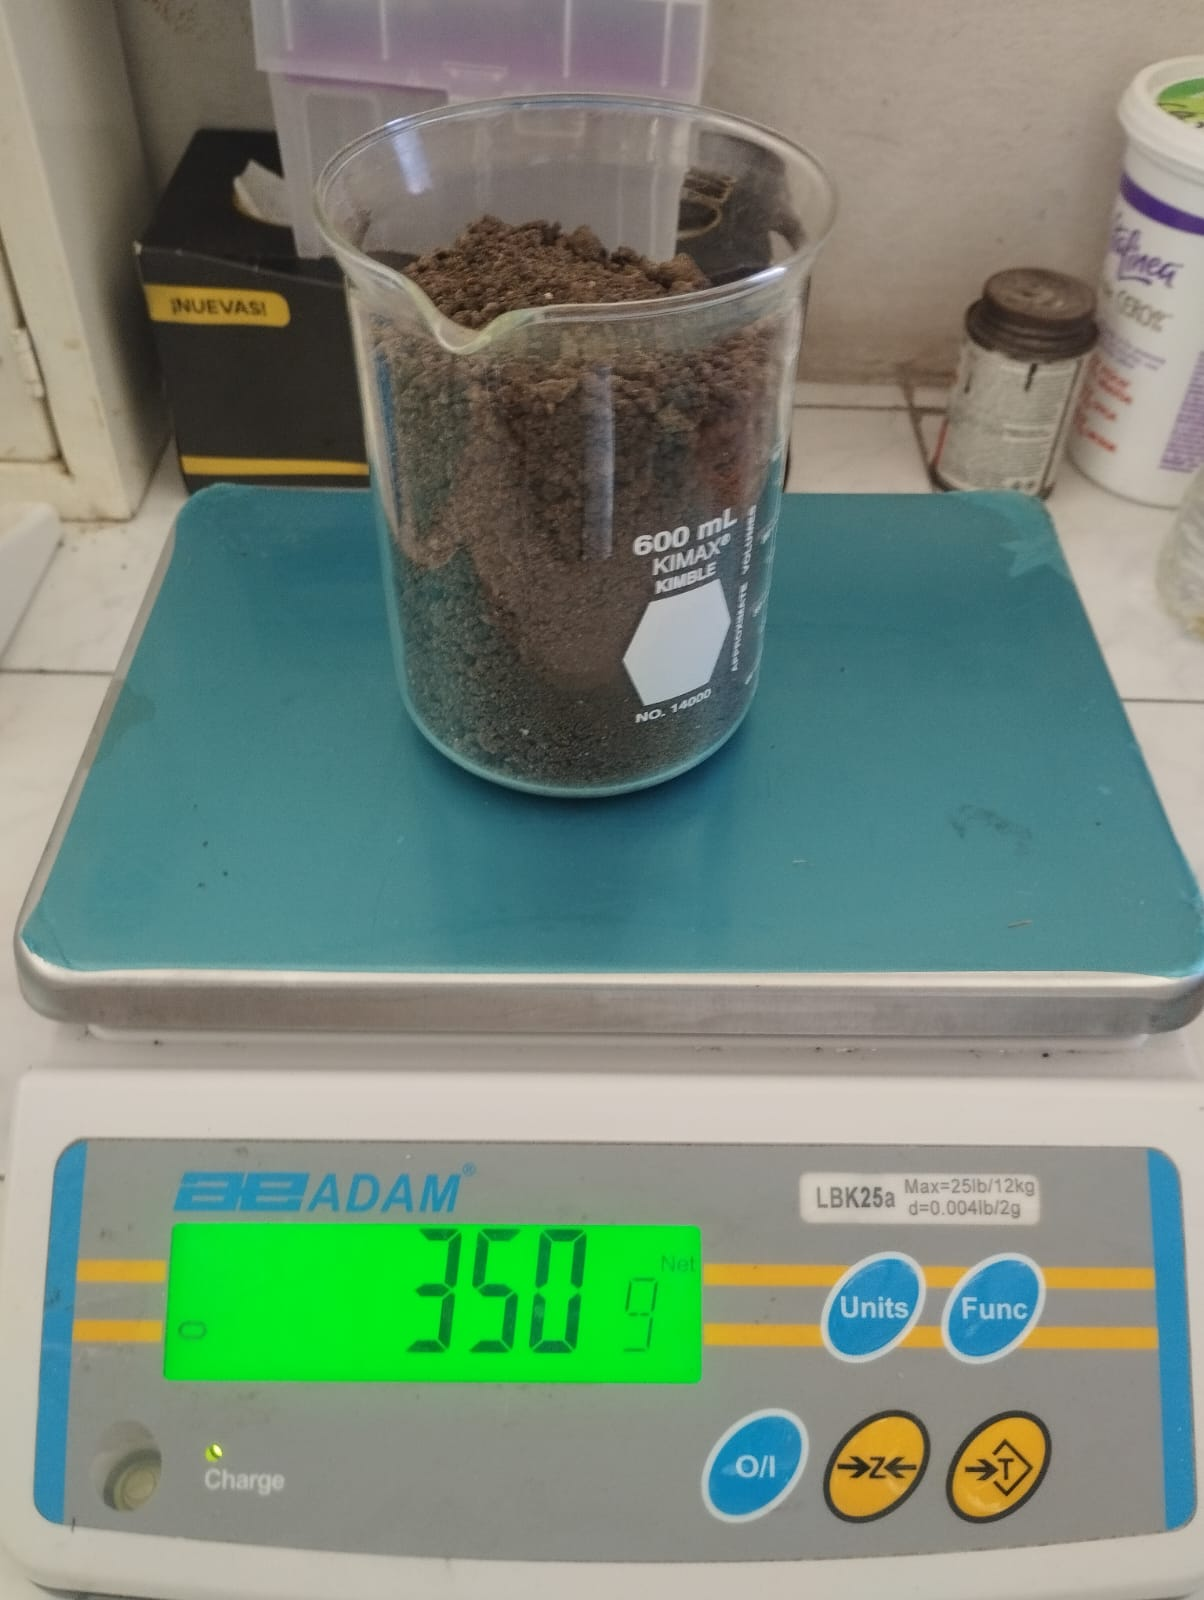
\includegraphics[width=3cm, height=5cm]{imagenes/humus}
				\caption{Pesaje del humus de lombriz con ayuda de una bascula.}
				\label{humus}
				\end{minipage}
			\end{figure}
			
			\textbf{3.}	Previo a su uso, el reactor se sometió a un proceso de limpieza exhaustiva (Figura~\ref{progra}), seguido de la aplicación estratégica de cinta de teflón en la zona roscada inferior para garantizar un sellado hermético. Finalmente, se procedió al ensamblaje mediante el apriete controlado del tornillo, asegurando así la integridad del sistema.
			
			
			
			\textbf{4.}	Se cargó el reactor con 6.0 L de agua desmineralizada, dosificados mediante un vaso de precipitado de 1 L, calibrado. Posteriormente, se incorporaron los 180 g de bagazo de caña previamente pesados y contenidos en la bolsa de 3 kg, siguiendo el procedimiento ilustrado en la Figura \ref{baciad}.
			

				\begin{figure}[H]
				\centering
				\begin{minipage}{0.46\textwidth}
					\centering
					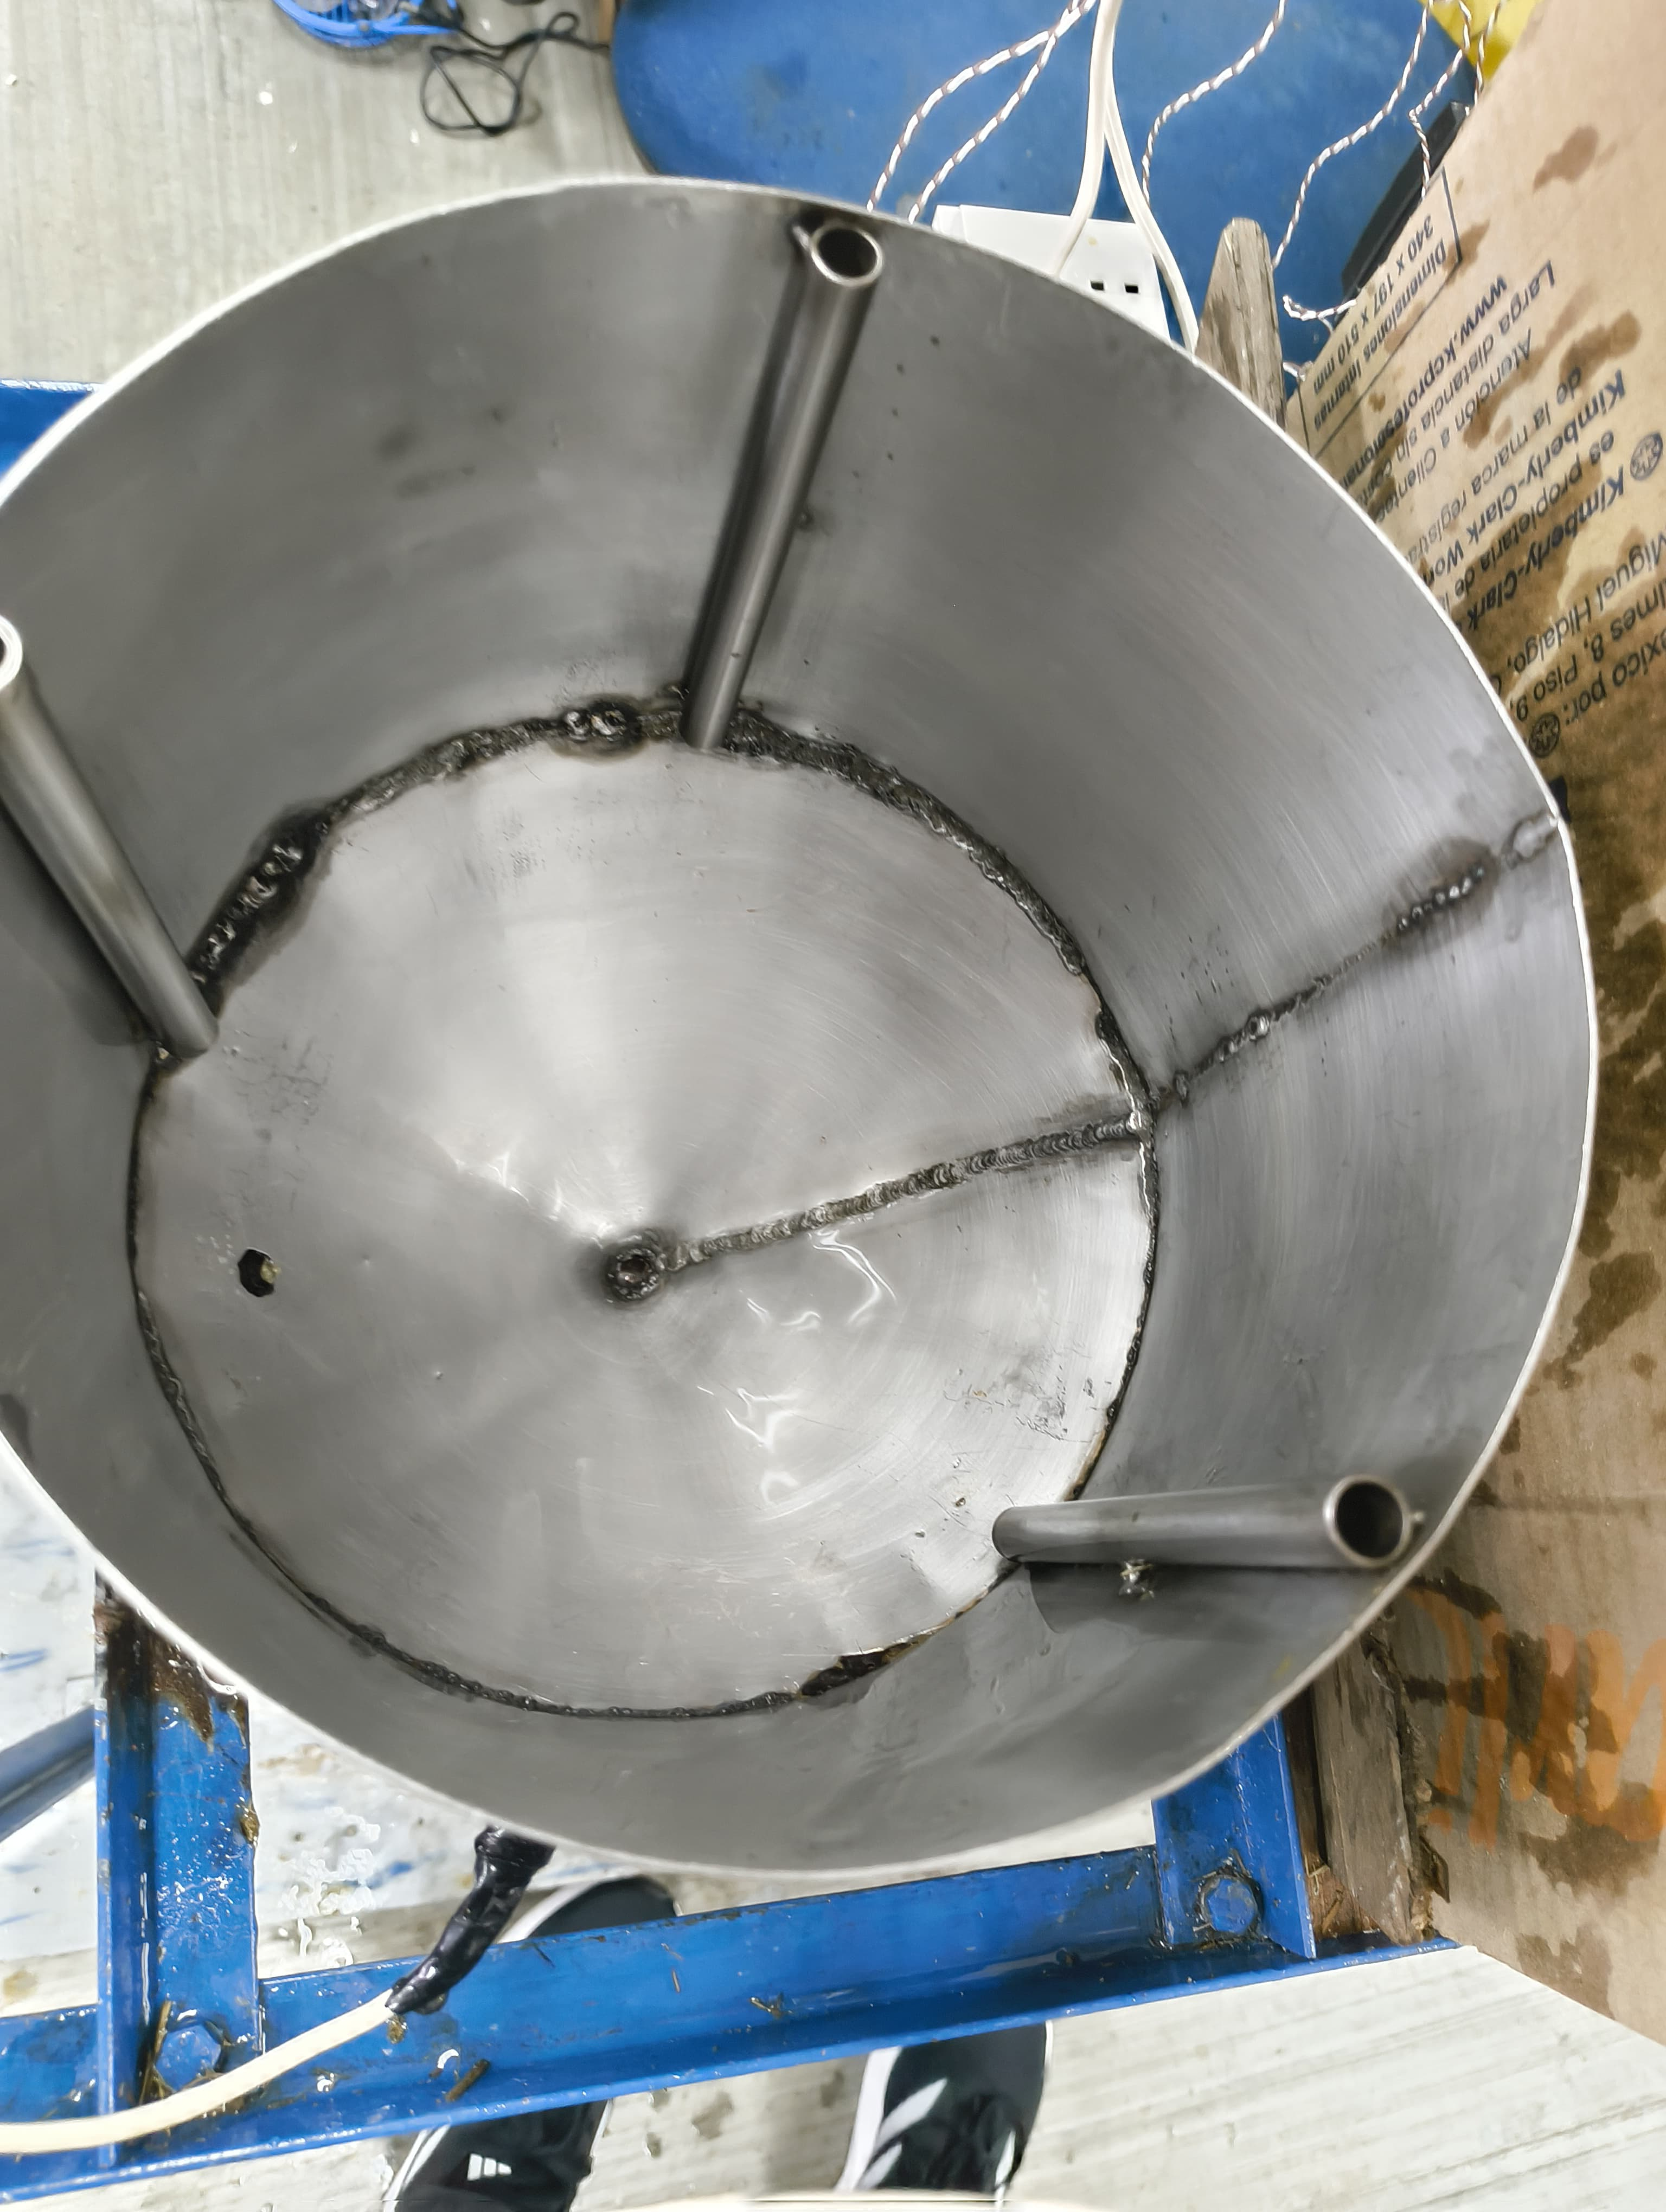
\includegraphics[width=4cm, height=5cm]{imagenes/reactor limpio} % Cambia "imagen1.jpg" por el nombre de tu archivo
					\caption{Fotografía muestra el reactor tipo batch después de limpiarlo.}
					\label{progra}
				\end{minipage}
				\hfill
				\begin{minipage}{0.48\textwidth}
					\centering
					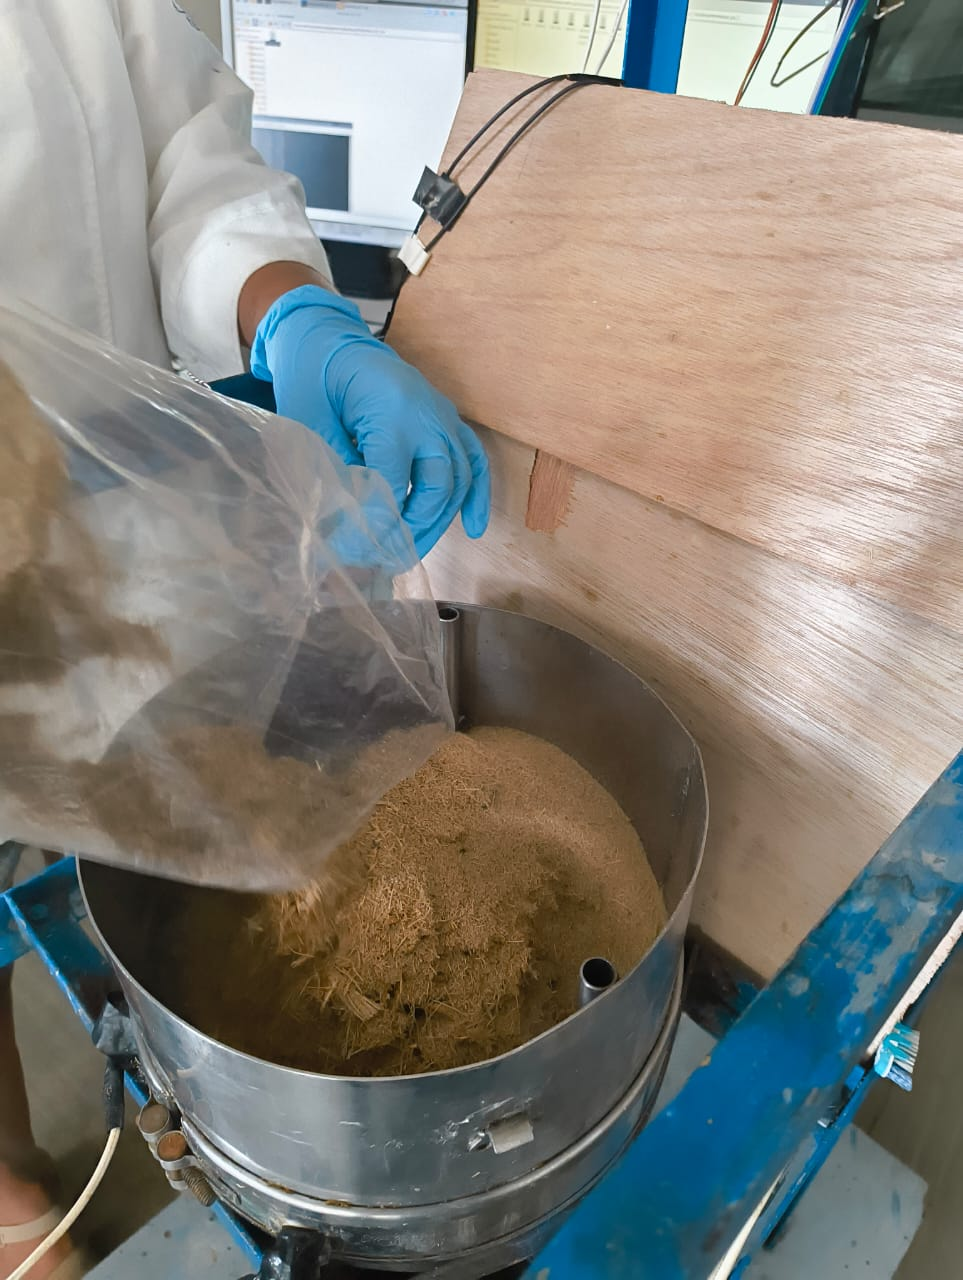
\includegraphics[width=4cm, height=5cm]{imagenes/biologico5} % Cambia "imagen2.jpg" por el nombre de tu archivo
					\caption{ Carga del bagazo de caña en el reactor tipo batch.}
					\label{baciad}
				\end{minipage}
			\end{figure}
			
			\textbf{5.}	Se adicionaron 300 g de humus de lombriz al reactor que ya contenía agua desmineralizada y bagazo de caña (Figura \ref{humus2}).
			

			\textbf{6.} Se procedió a sellar el reactor utilizando una tapa que incorpora el motor. Se colocaron los sensores de tipo termopar K en los tubos de un centímetro de diámetro, asegurándo que estuvieran correctamente posicionados. Para evitar fugas de vapor, se utilizó algodón para sellar adecuadamente los tubos. Además, se emplearon láminas de aluminio y cinta aislante o térmica para garantizar un cierre hermético tanto alrededor de la tapa como en la zona de los sensores, tal como se observa en la Figura~\ref{cellado del reactor}.
			
		
			
	\begin{figure}[H]
		\centering
		\begin{minipage}{0.46\textwidth}
			\centering
			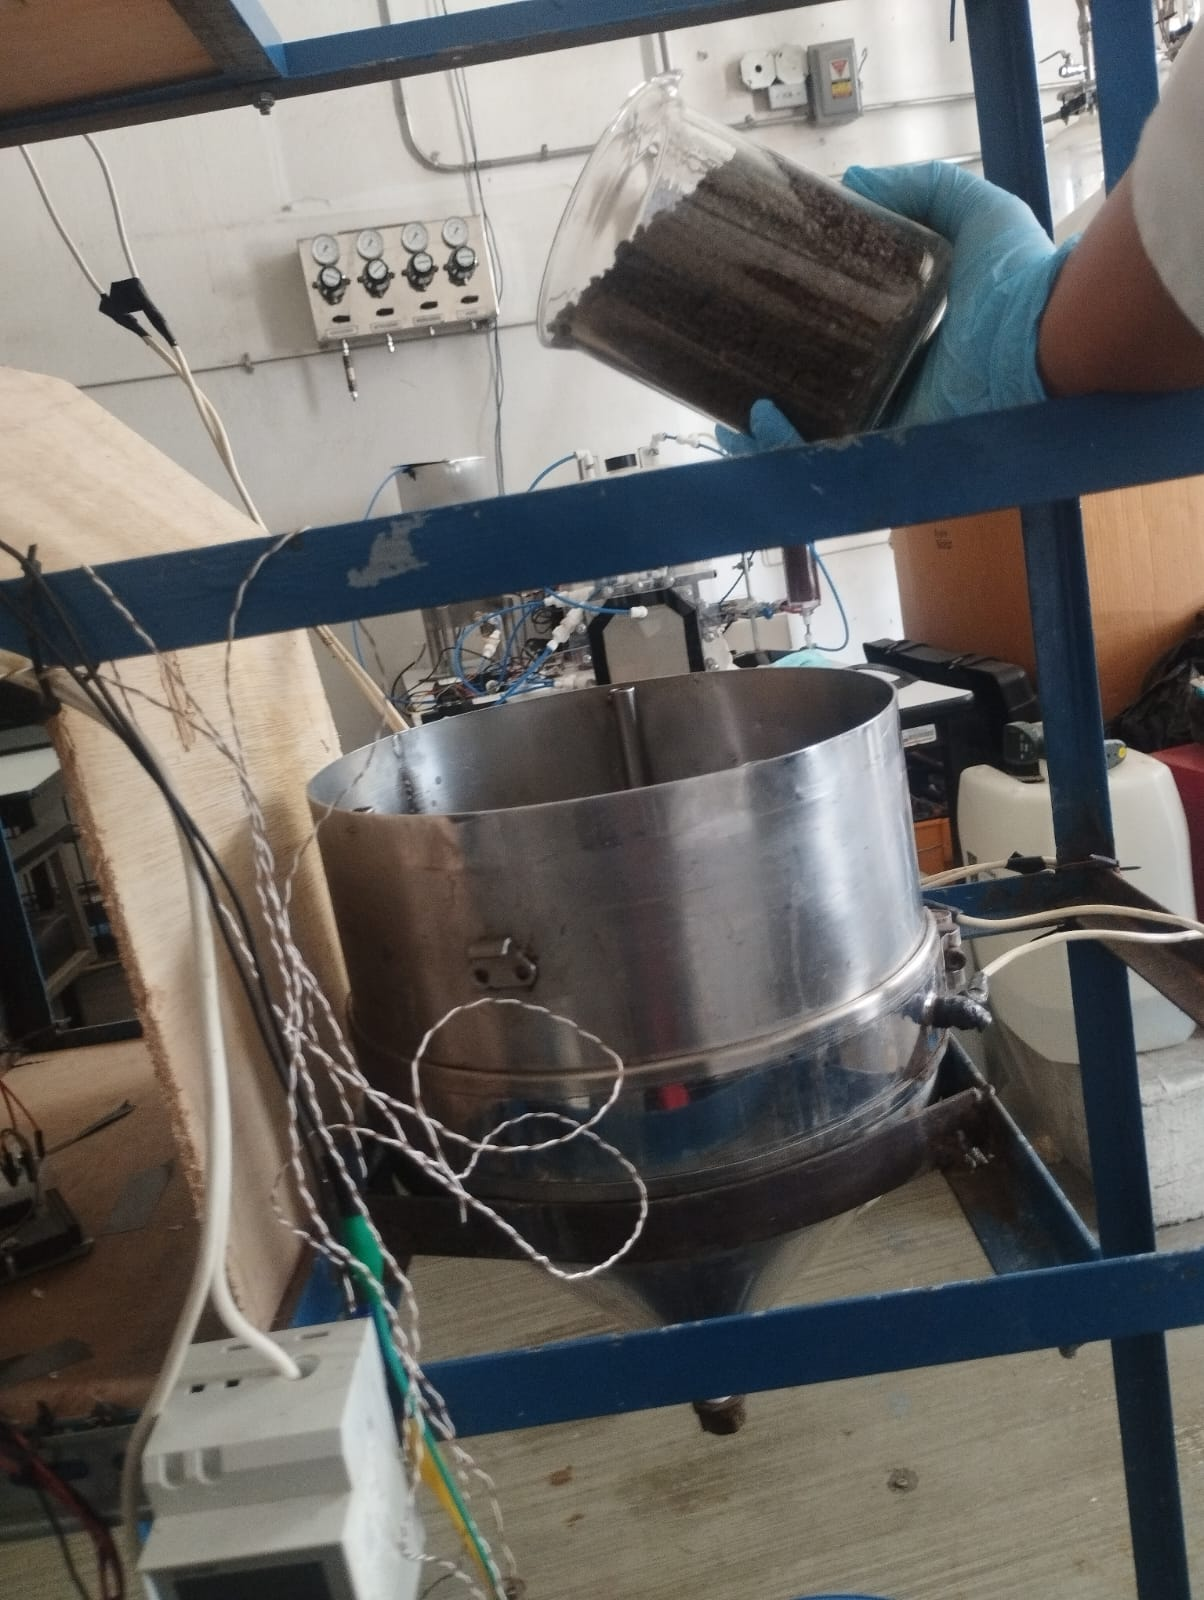
\includegraphics[width=3cm, height=5cm]{imagenes/humus2} % Cambia "imagen1.jpg" por el nombre de tu archivo
			\caption{Fotografía que muestra como se le agrega el humus de lombriz al reactor.}
				\label{humus2}
			\end{minipage}
			\hfill
			\begin{minipage}{0.48\textwidth}
				\centering
				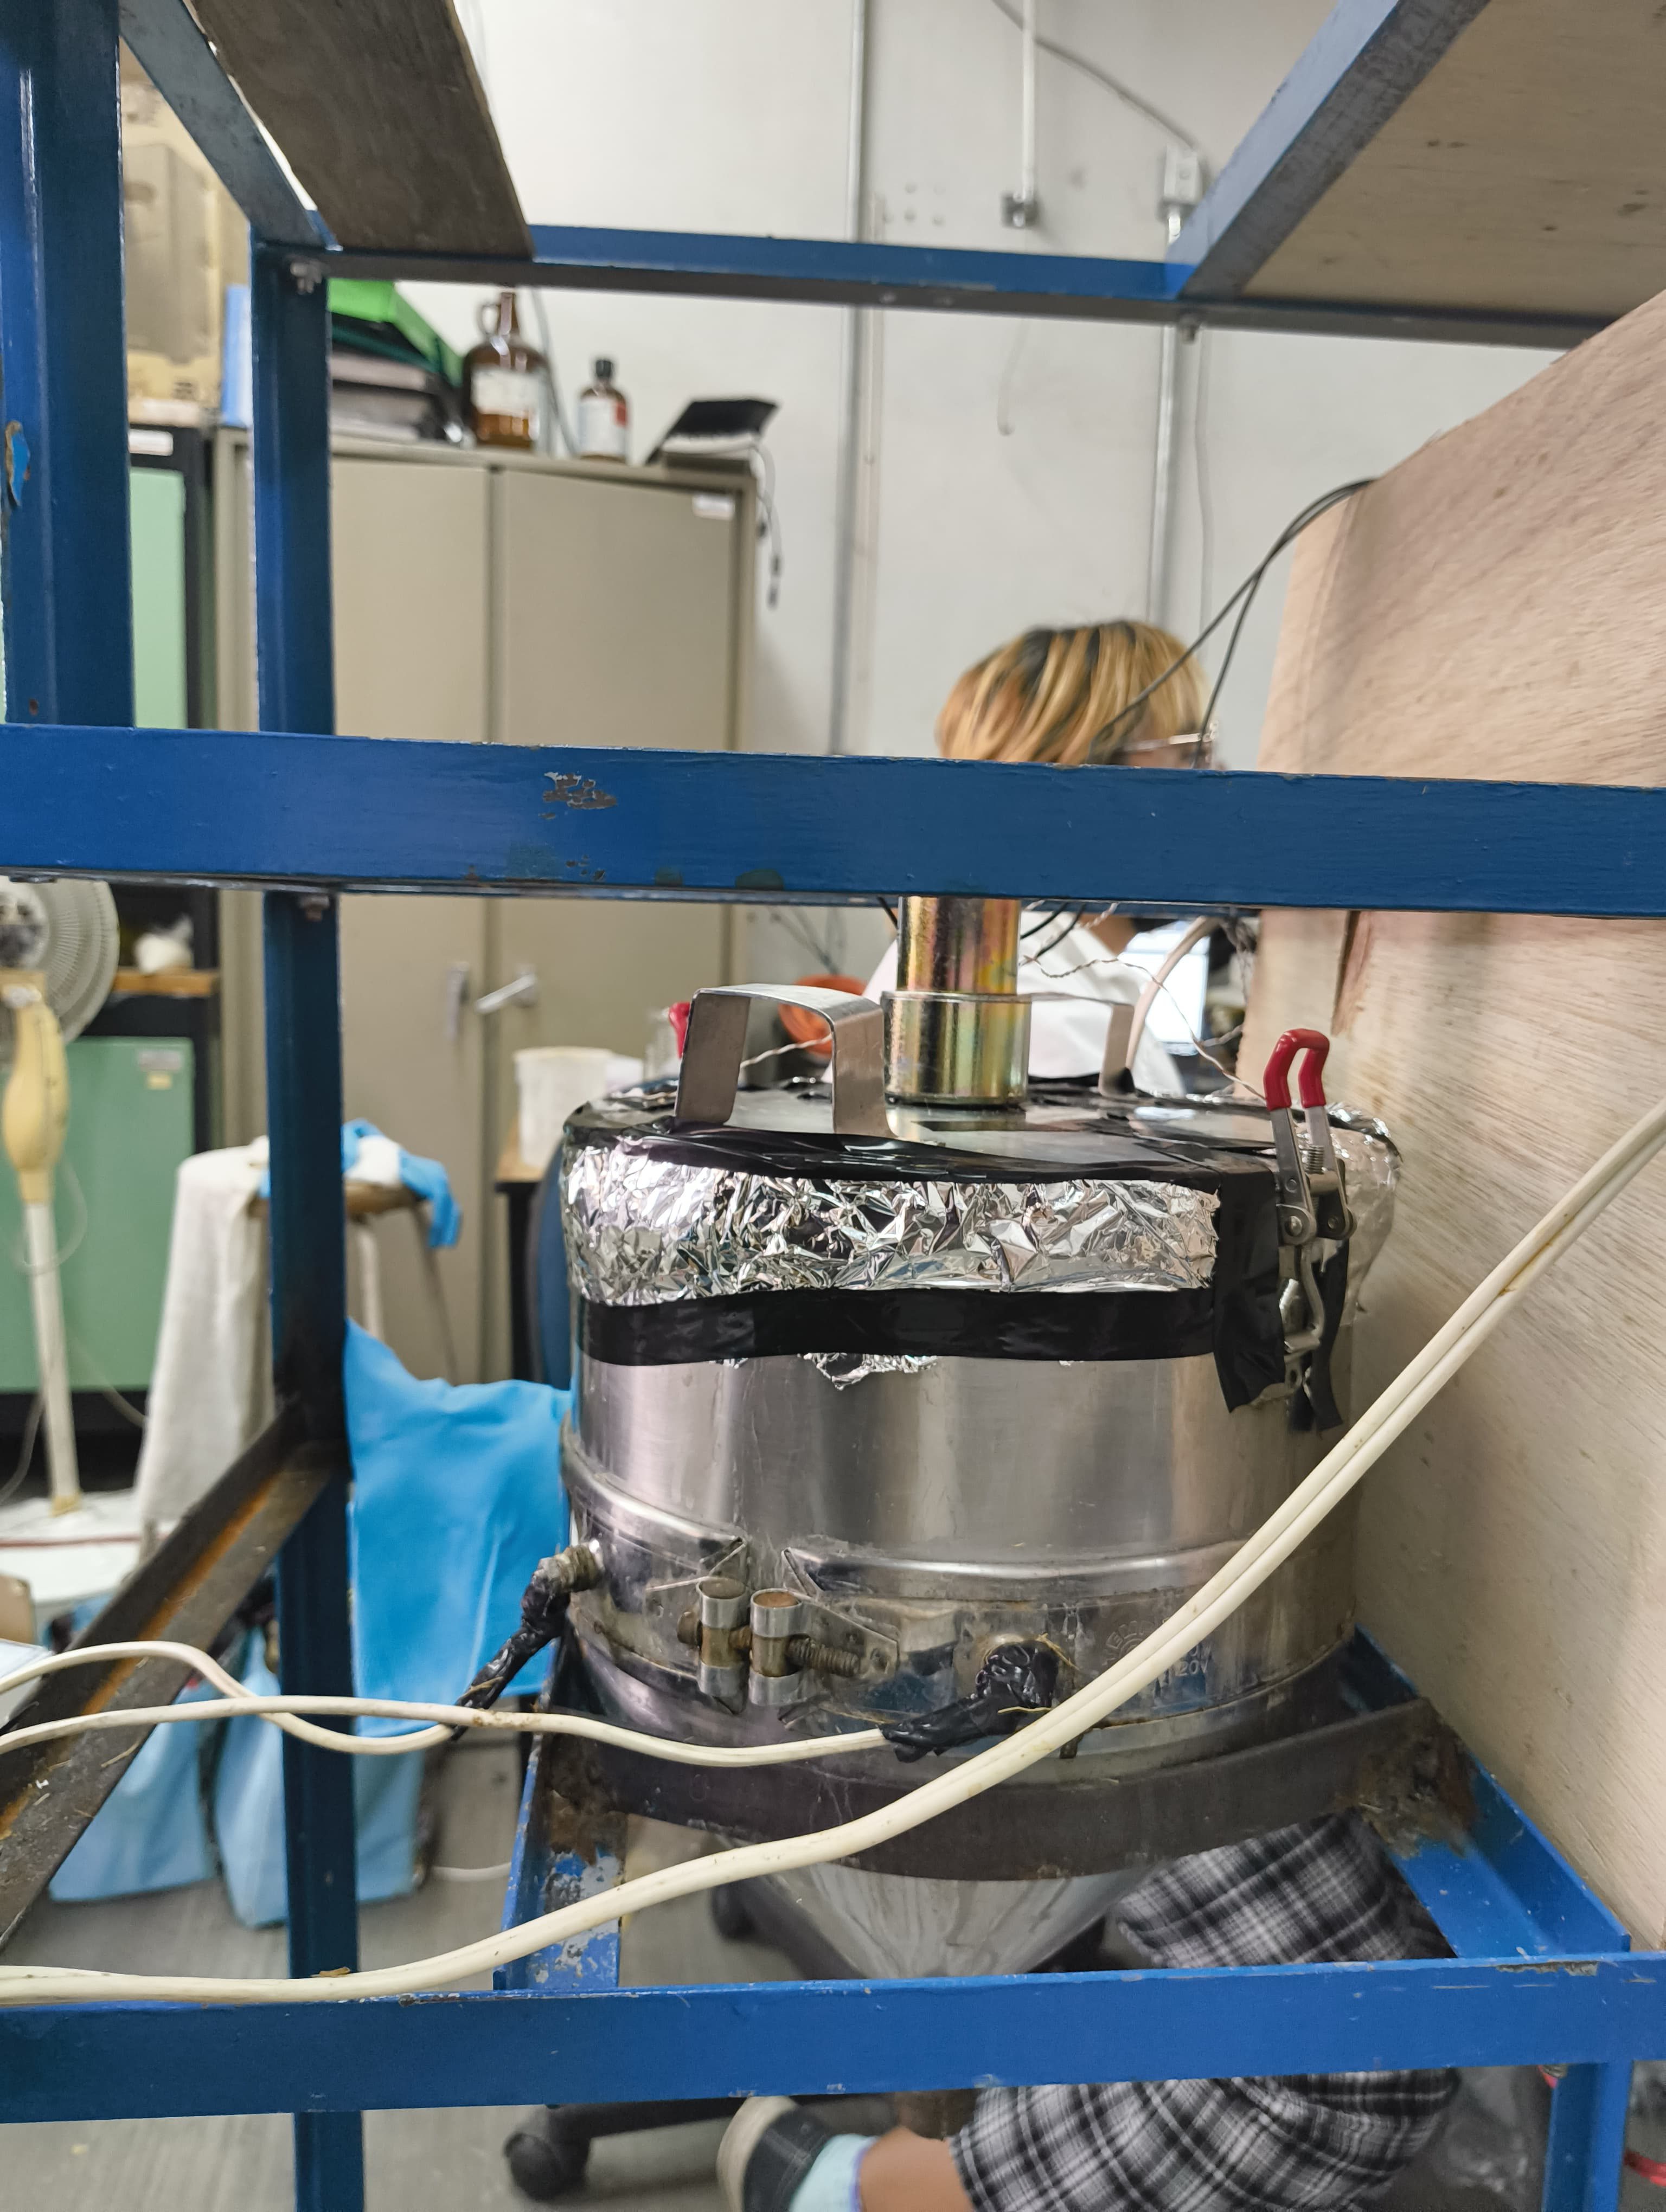
\includegraphics[width=3cm, height=5cm]{imagenes/cellado del reactor} % Cambia "imagen2.jpg" por el nombre de tu archivo
				\caption{Esta fotografía muestra el reactor después de sellarlo.}
				\label{cellado del reactor}
			\end{minipage}
		\end{figure}
		
			
			\textbf{7. } Se procedió a conectar las Raspberry Pi y los monitores, así como las fuentes de alimentación y el sistema de respaldo (no-break). Se conectaron los contactos múltiples necesarios, se configuraron los dispositivos y se programó el control para mantener la temperatura conforme al diseño experimental descrito en el apartado \ref{DiseñopretratamientoBioogico}. El proceso se mantuvo durante el tiempo estipulado para el pretratamiento. El diseño del control de temperatura se reporta en el anexo \ref{diseño del control de temp}. Las Figuras \ref{progra 1} y \ref{progra 2} muestran las pantallas con el control en funcionamiento.
			
			\begin{figure}[H]
				\centering
				\begin{minipage}{0.46\textwidth}
					\centering
					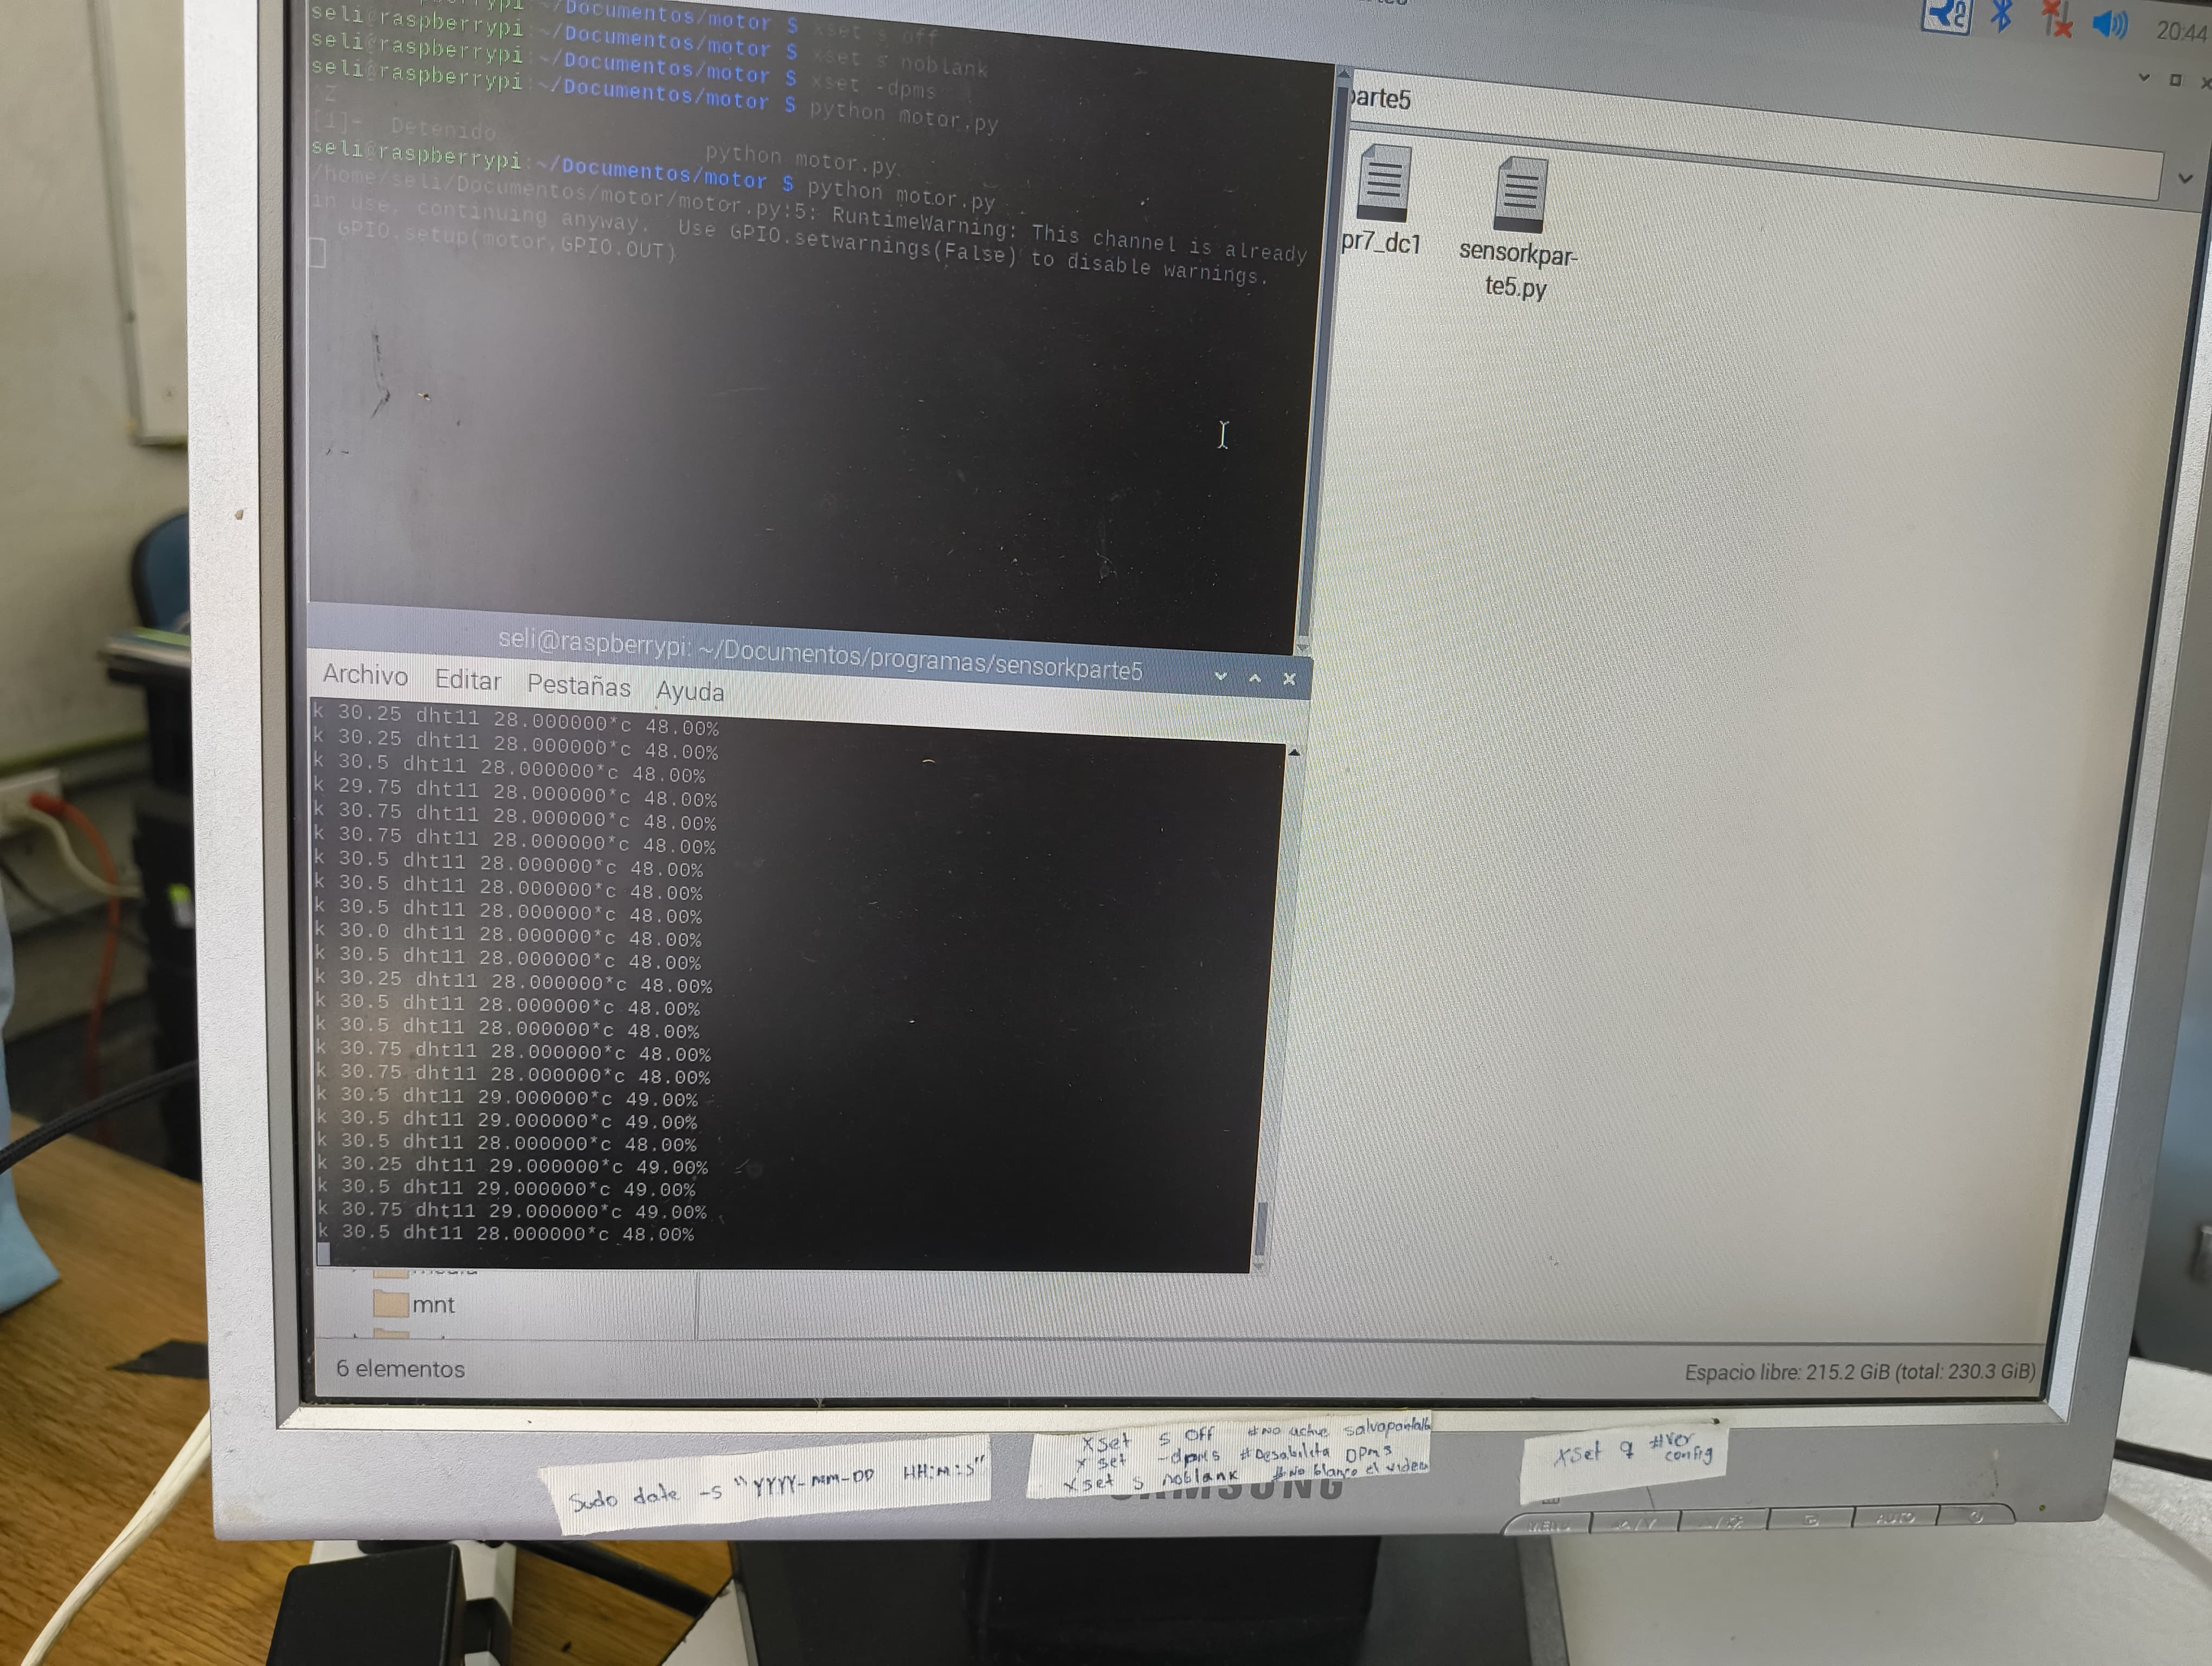
\includegraphics[width=5cm, height=3cm]{imagenes/programa1} % Cambia "imagen1.jpg" por el nombre de tu archivo
					\caption{Programa de la temperatura ambiente en marcha.}
					\label{progra 1}
				\end{minipage}
				\hfill
				\begin{minipage}{0.48\textwidth}
					\centering
					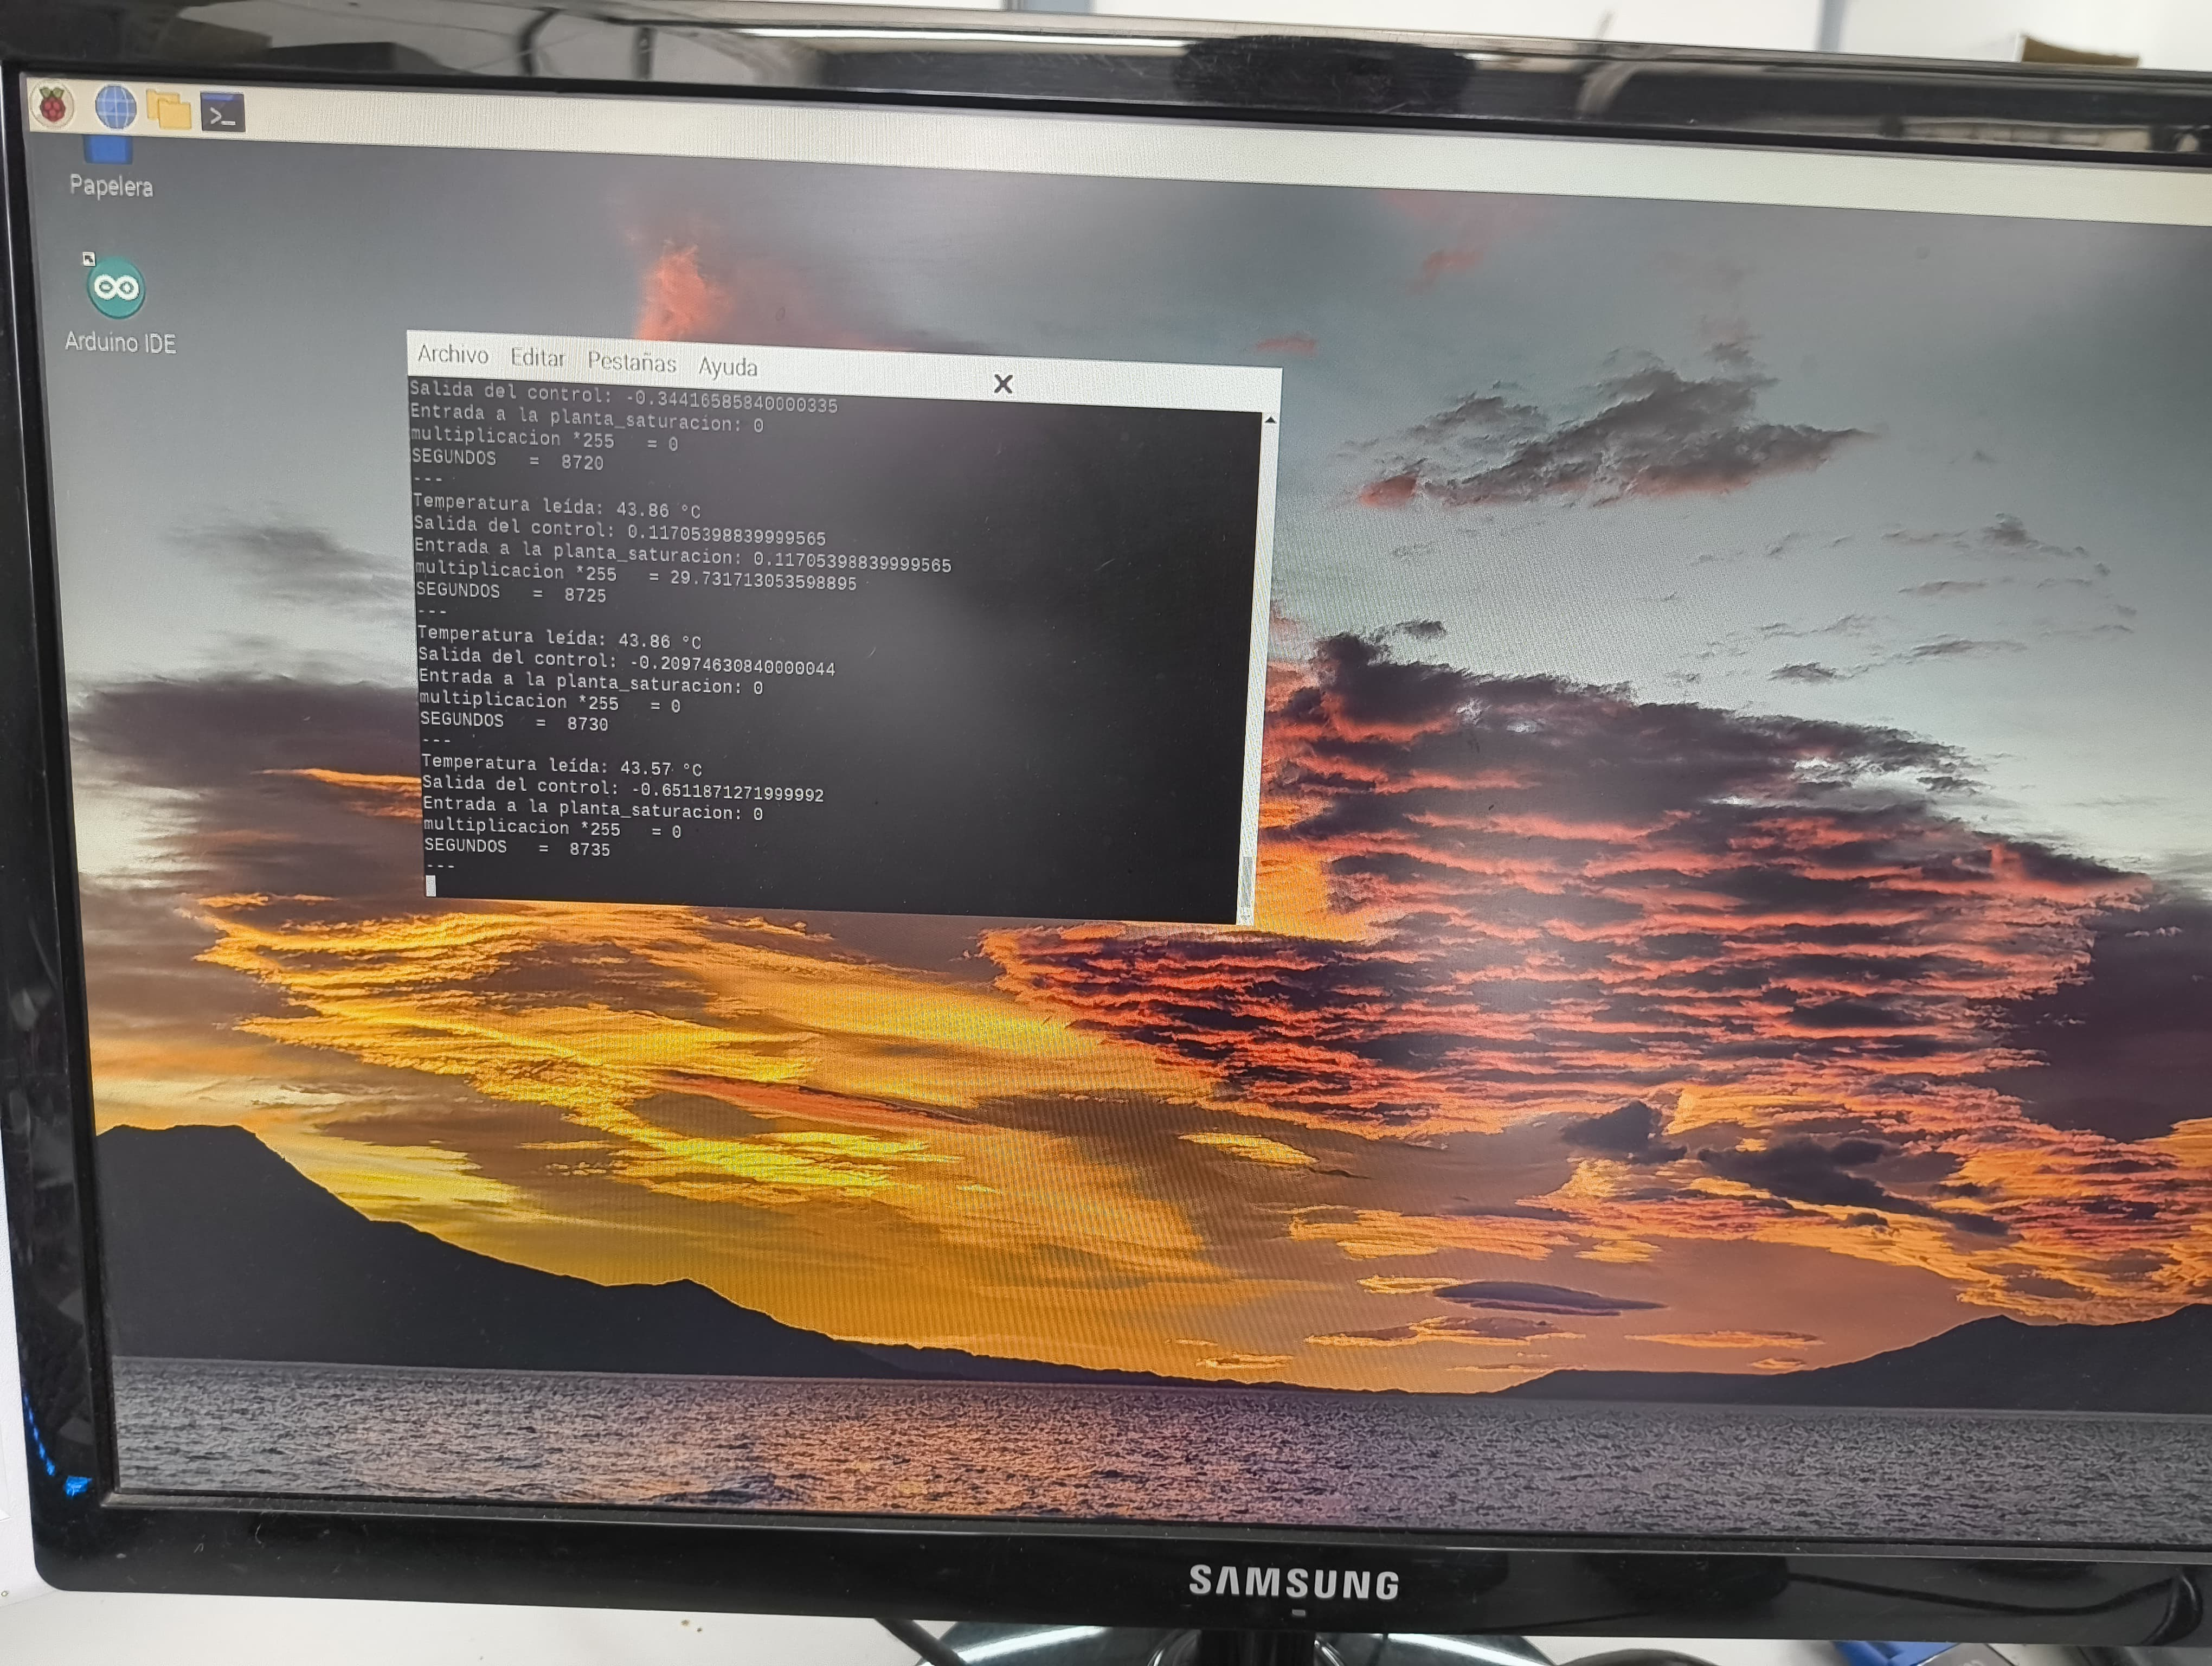
\includegraphics[width=5cm, height=3cm]{imagenes/programa2} % Cambia "imagen2.jpg" por el nombre de tu archivo
					\caption{Programa del control en marcha.}
					\label{progra 2}
				\end{minipage}
			\end{figure}
			

			
			%%%%%%%%%%%%%%%%%%%%%%%%%%%%%%%%%%%%%%%%%%%%%%%%%%%%%%%%%%%%%%%%%%%%%%%%%%%%%%%%%%%%%%%%%%%%%%%%%%%%%%%%%%%%%%%%%%%%%%%%%%%%%%%%%%%%%%%%%
			
			\subsubsection{Pretratamiento Alcalino}
			El pretratamiento alcalino de la biomasa se implementó usando Hidróxido de Sodio. A continuación se muestran los insumos y los pasos para llevar a cabo las pruebas experimentales.		
			\\[1 em]
			\textbf{Compuestos} 
			\\[0.5em]
			
			\begin{tabular}{p{0.3\textwidth}p{0.3\textwidth}}
				\textcolor{blue}{$\bullet$} \textit{Hidróxido de sodio} &	\textcolor{blue}{$\bullet$}\textit{ Bagazo de caña} 
			\end{tabular} \\[ 1em]
			
			
			
			\textbf{Materiales} 
			\\[1 em]
			
			\begin{tabular}{p{0.3\textwidth}p{0.3\textwidth}p{0.3\textwidth}}
				$\bullet$ \textit{Agua desmineralizada }& $\bullet$ \textit{Algodón }& $\bullet$ \textit{Bolsa plástica de 30×40 cm} \\
				$\bullet$ \textit{Báscula} & $\bullet$ \textit{Cinta aislante} & $\bullet$ \textit{Cinta de teflón}
			\end{tabular}
			\\[0.5em]
			
			
			\textbf{Procedimiento}
			\\[0.5em]
			
			\textbf{1.}	La cantidad de bagazo se determinó mediante pesaje con báscula digital (precisión ±0.2 g) usando una bolsa plástica de 30×40 cm como contenedor, hasta alcanzar 180 g. Alternativamente, cuando se requirió la medida de 1 cm, se utilizó directamente el material preclasificado y calibrado, según se ilustra en la Figura \ref{bagazo1}.\\
			
			\textbf{2.} Mediante una báscula digital (precisión ±0.2 g) y vaso de precipitado de vidrio, se pesaron exactamente 120 g de hidróxido de sodio en pellets, asegurando la exactitud requerida para el proceso.Ver Figura \ref{cernir_bagazo_hidroxidopesado}.
			
			
			\begin{figure}[H]
				\centering
				\begin{minipage}{0.46\textwidth}
					\centering
					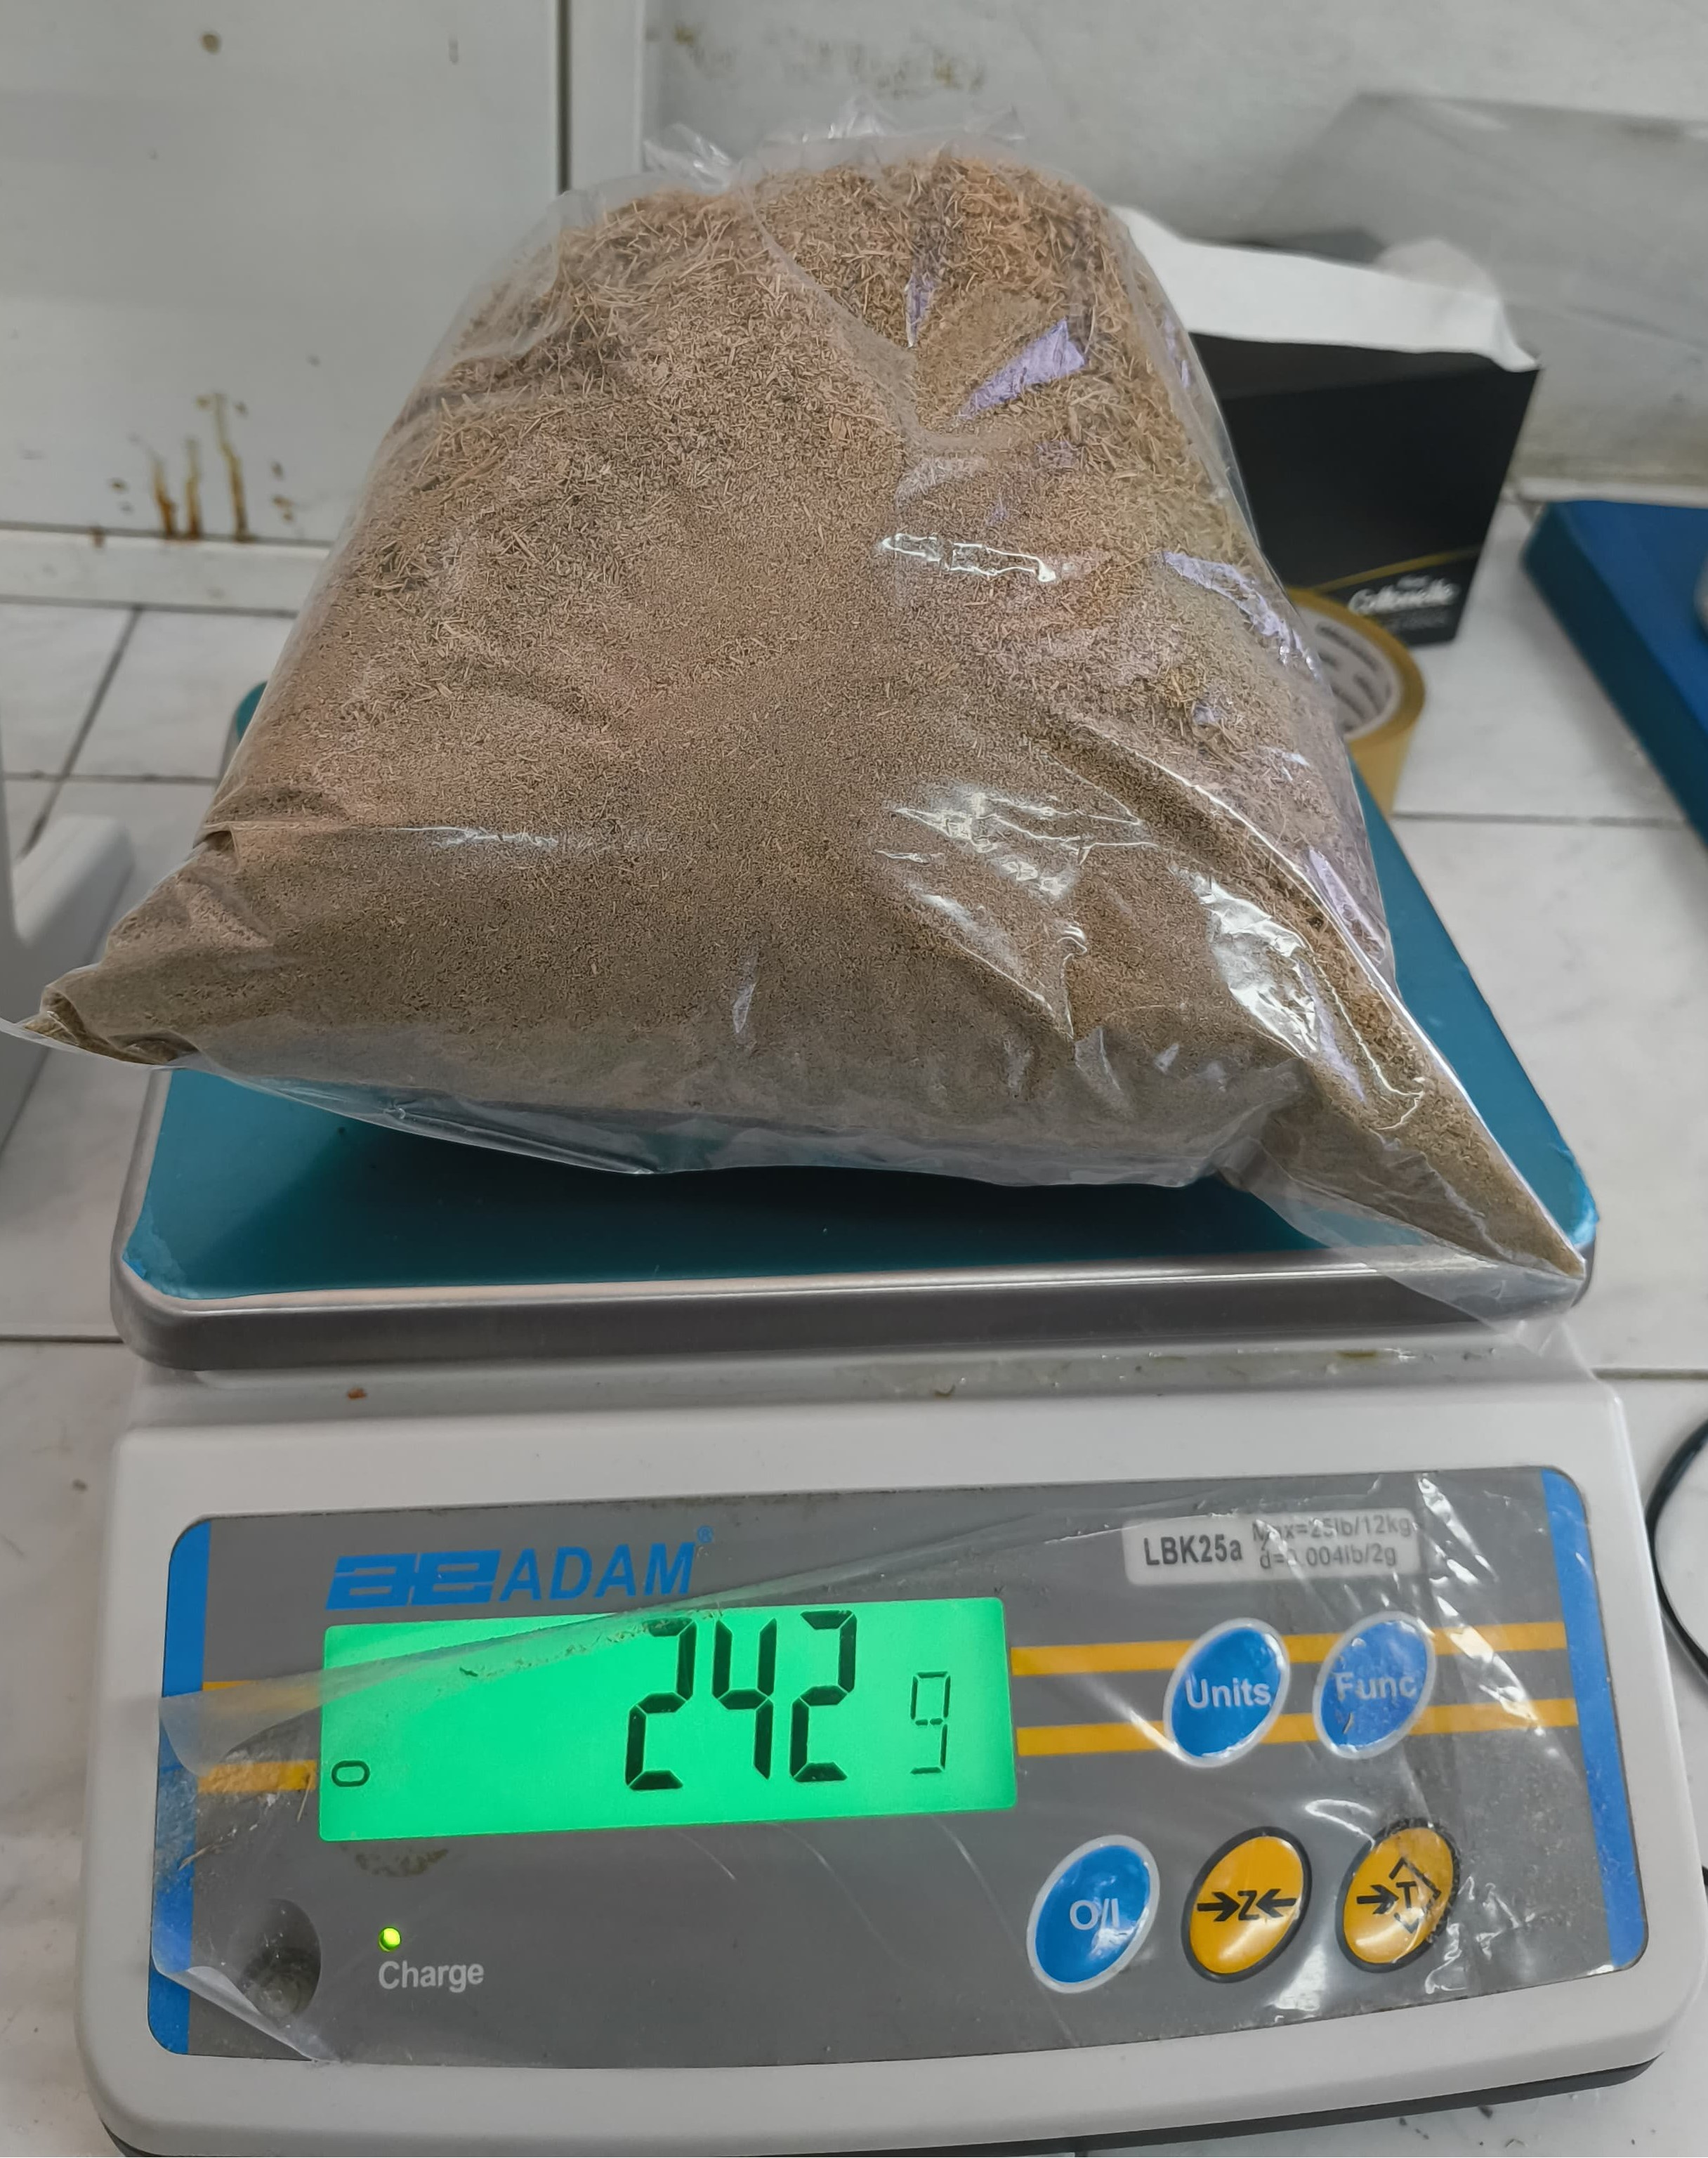
\includegraphics[width=3cm, height=5cm]{imagenes/pesado4}
					\caption{Bagazo de 1 cm.}
					\label{bagazo1}
				\end{minipage}
				\hfill
				\begin{minipage}{0.48\textwidth}
					\centering
					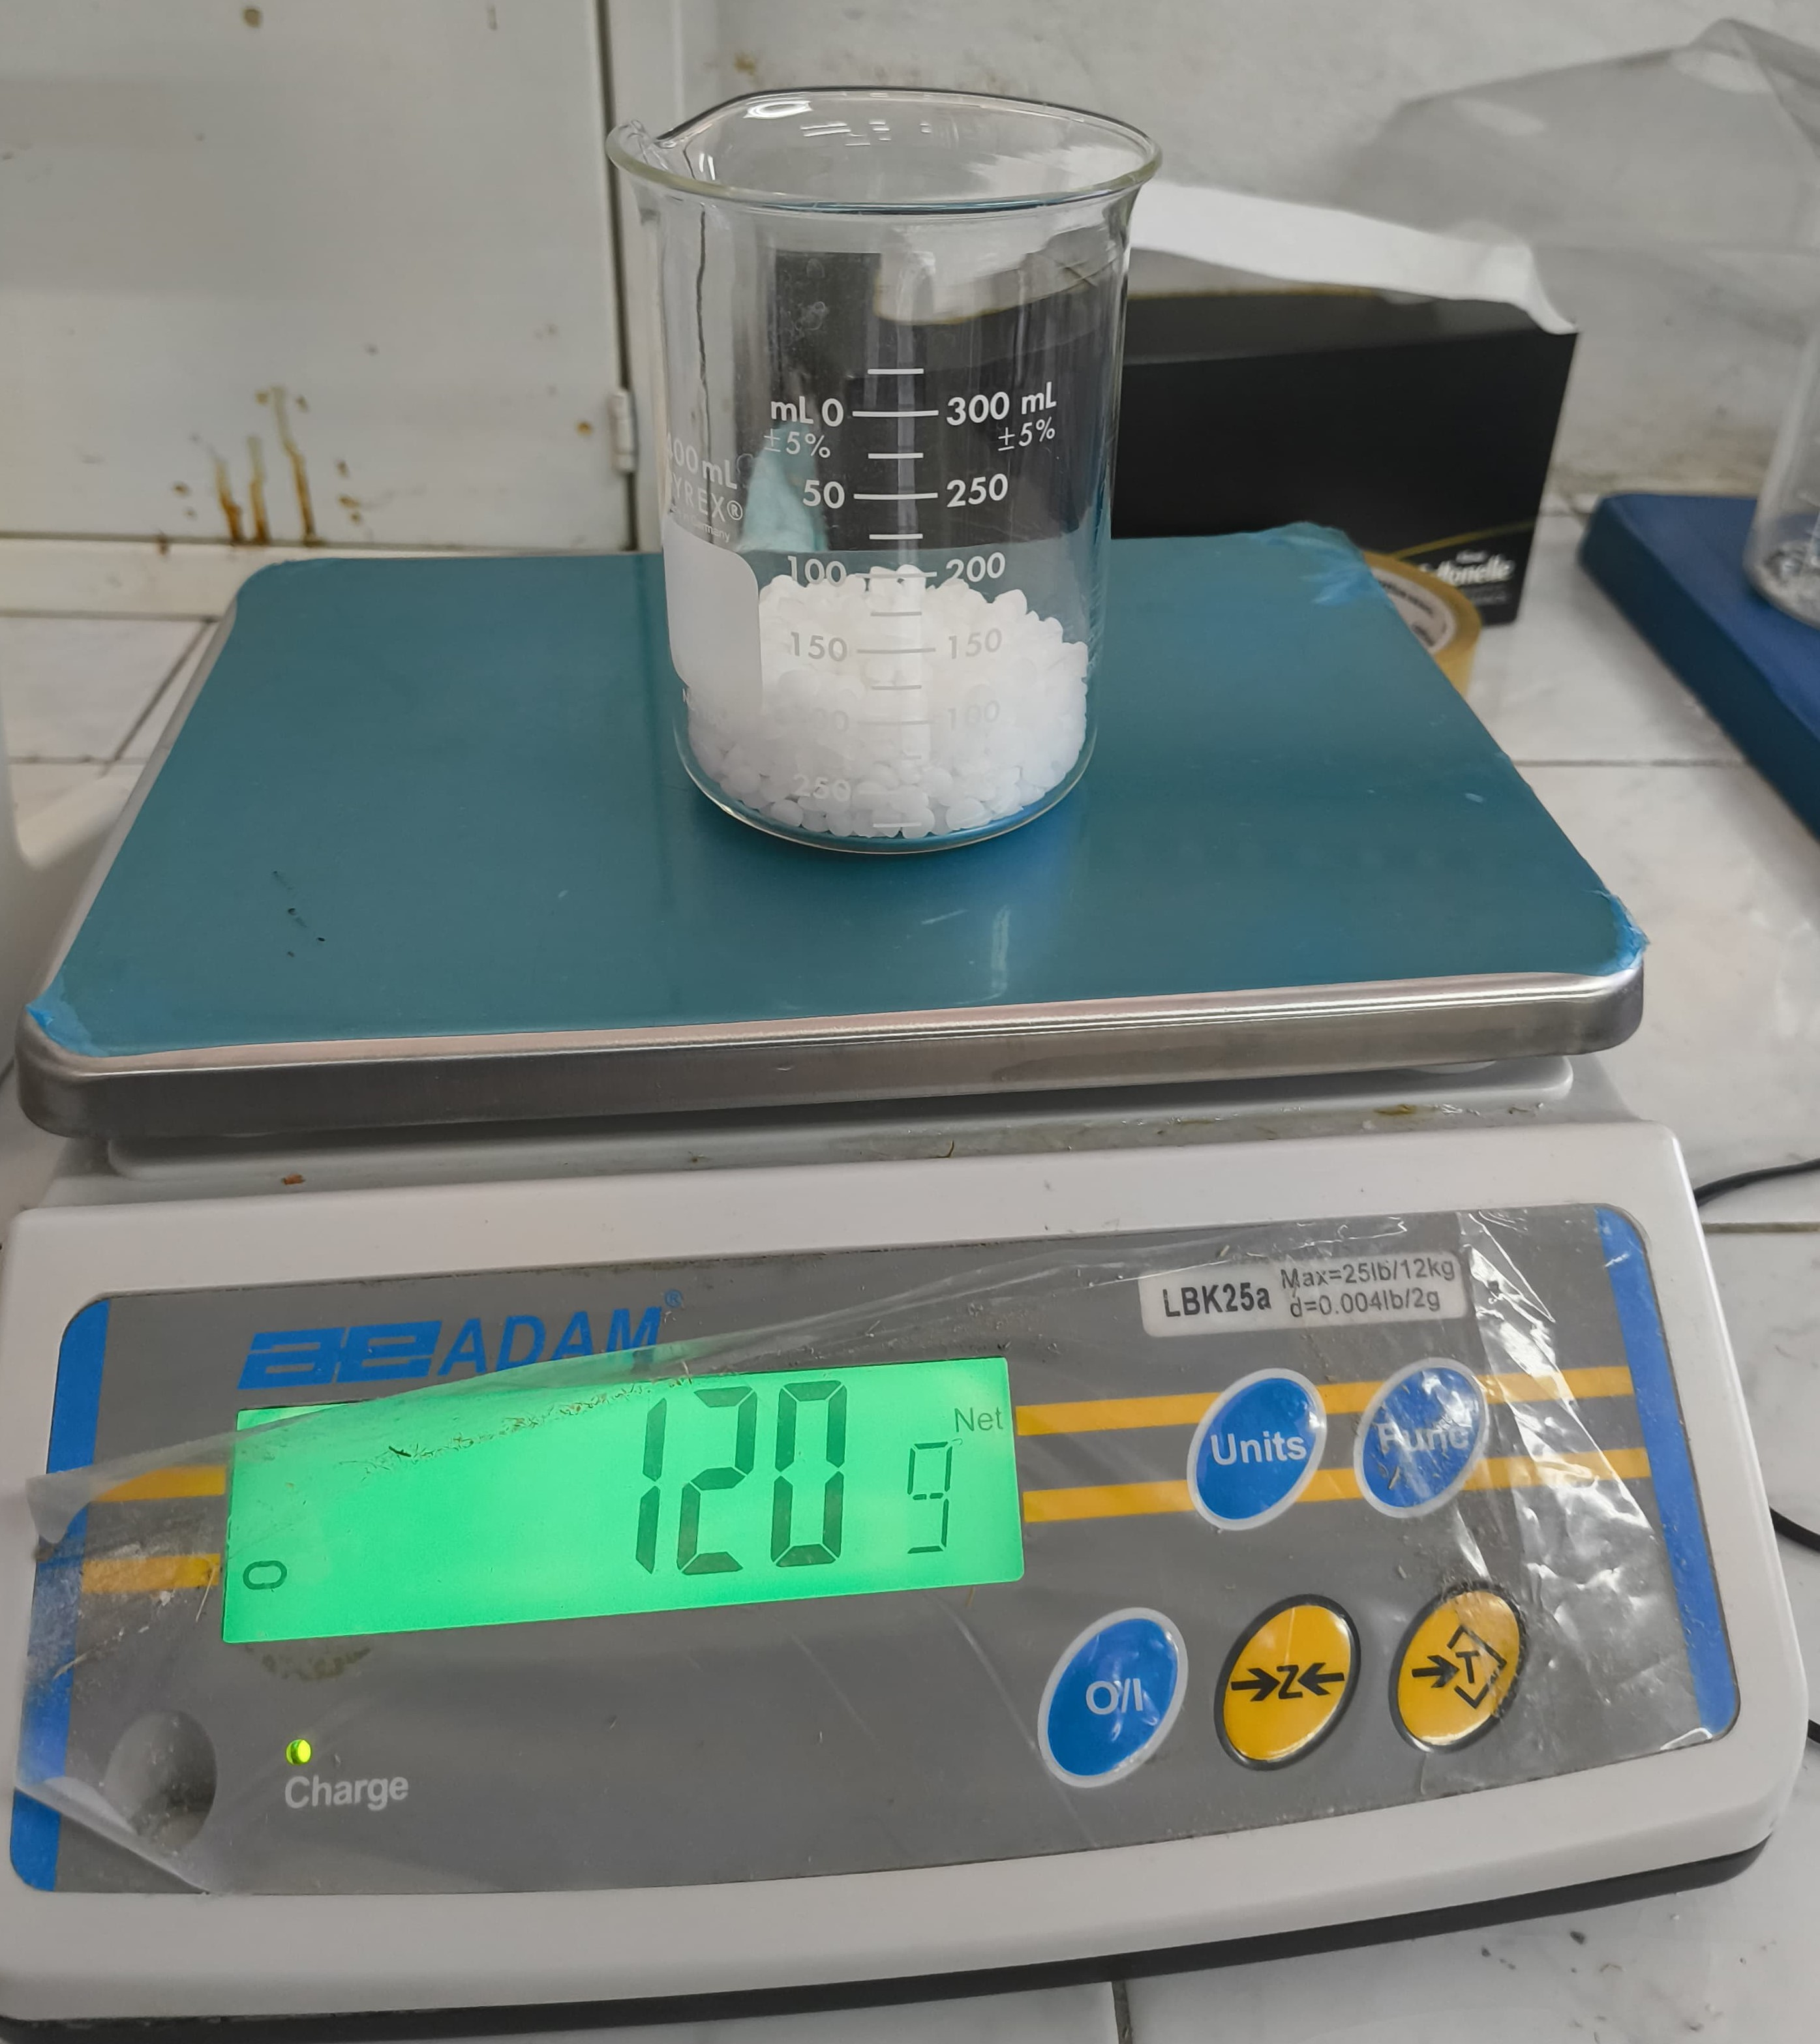
\includegraphics[width=3cm, height=5cm]{imagenes/hidroxido_pesado}
					\caption{El hidroxido es pesado en una bascula.}
					\label{cernir_bagazo_hidroxidopesado}
				\end{minipage}
			\end{figure}
			
			
			
			\textbf{3.} El reactor y su mezclador fueron enjuagados minuciosamente con agua desmineralizada para garantizar su limpieza óptima antes de ser usado, eliminando cualquier residuo que puediera afectar el proceso.
			\begin{figure} [H]
				\centering
				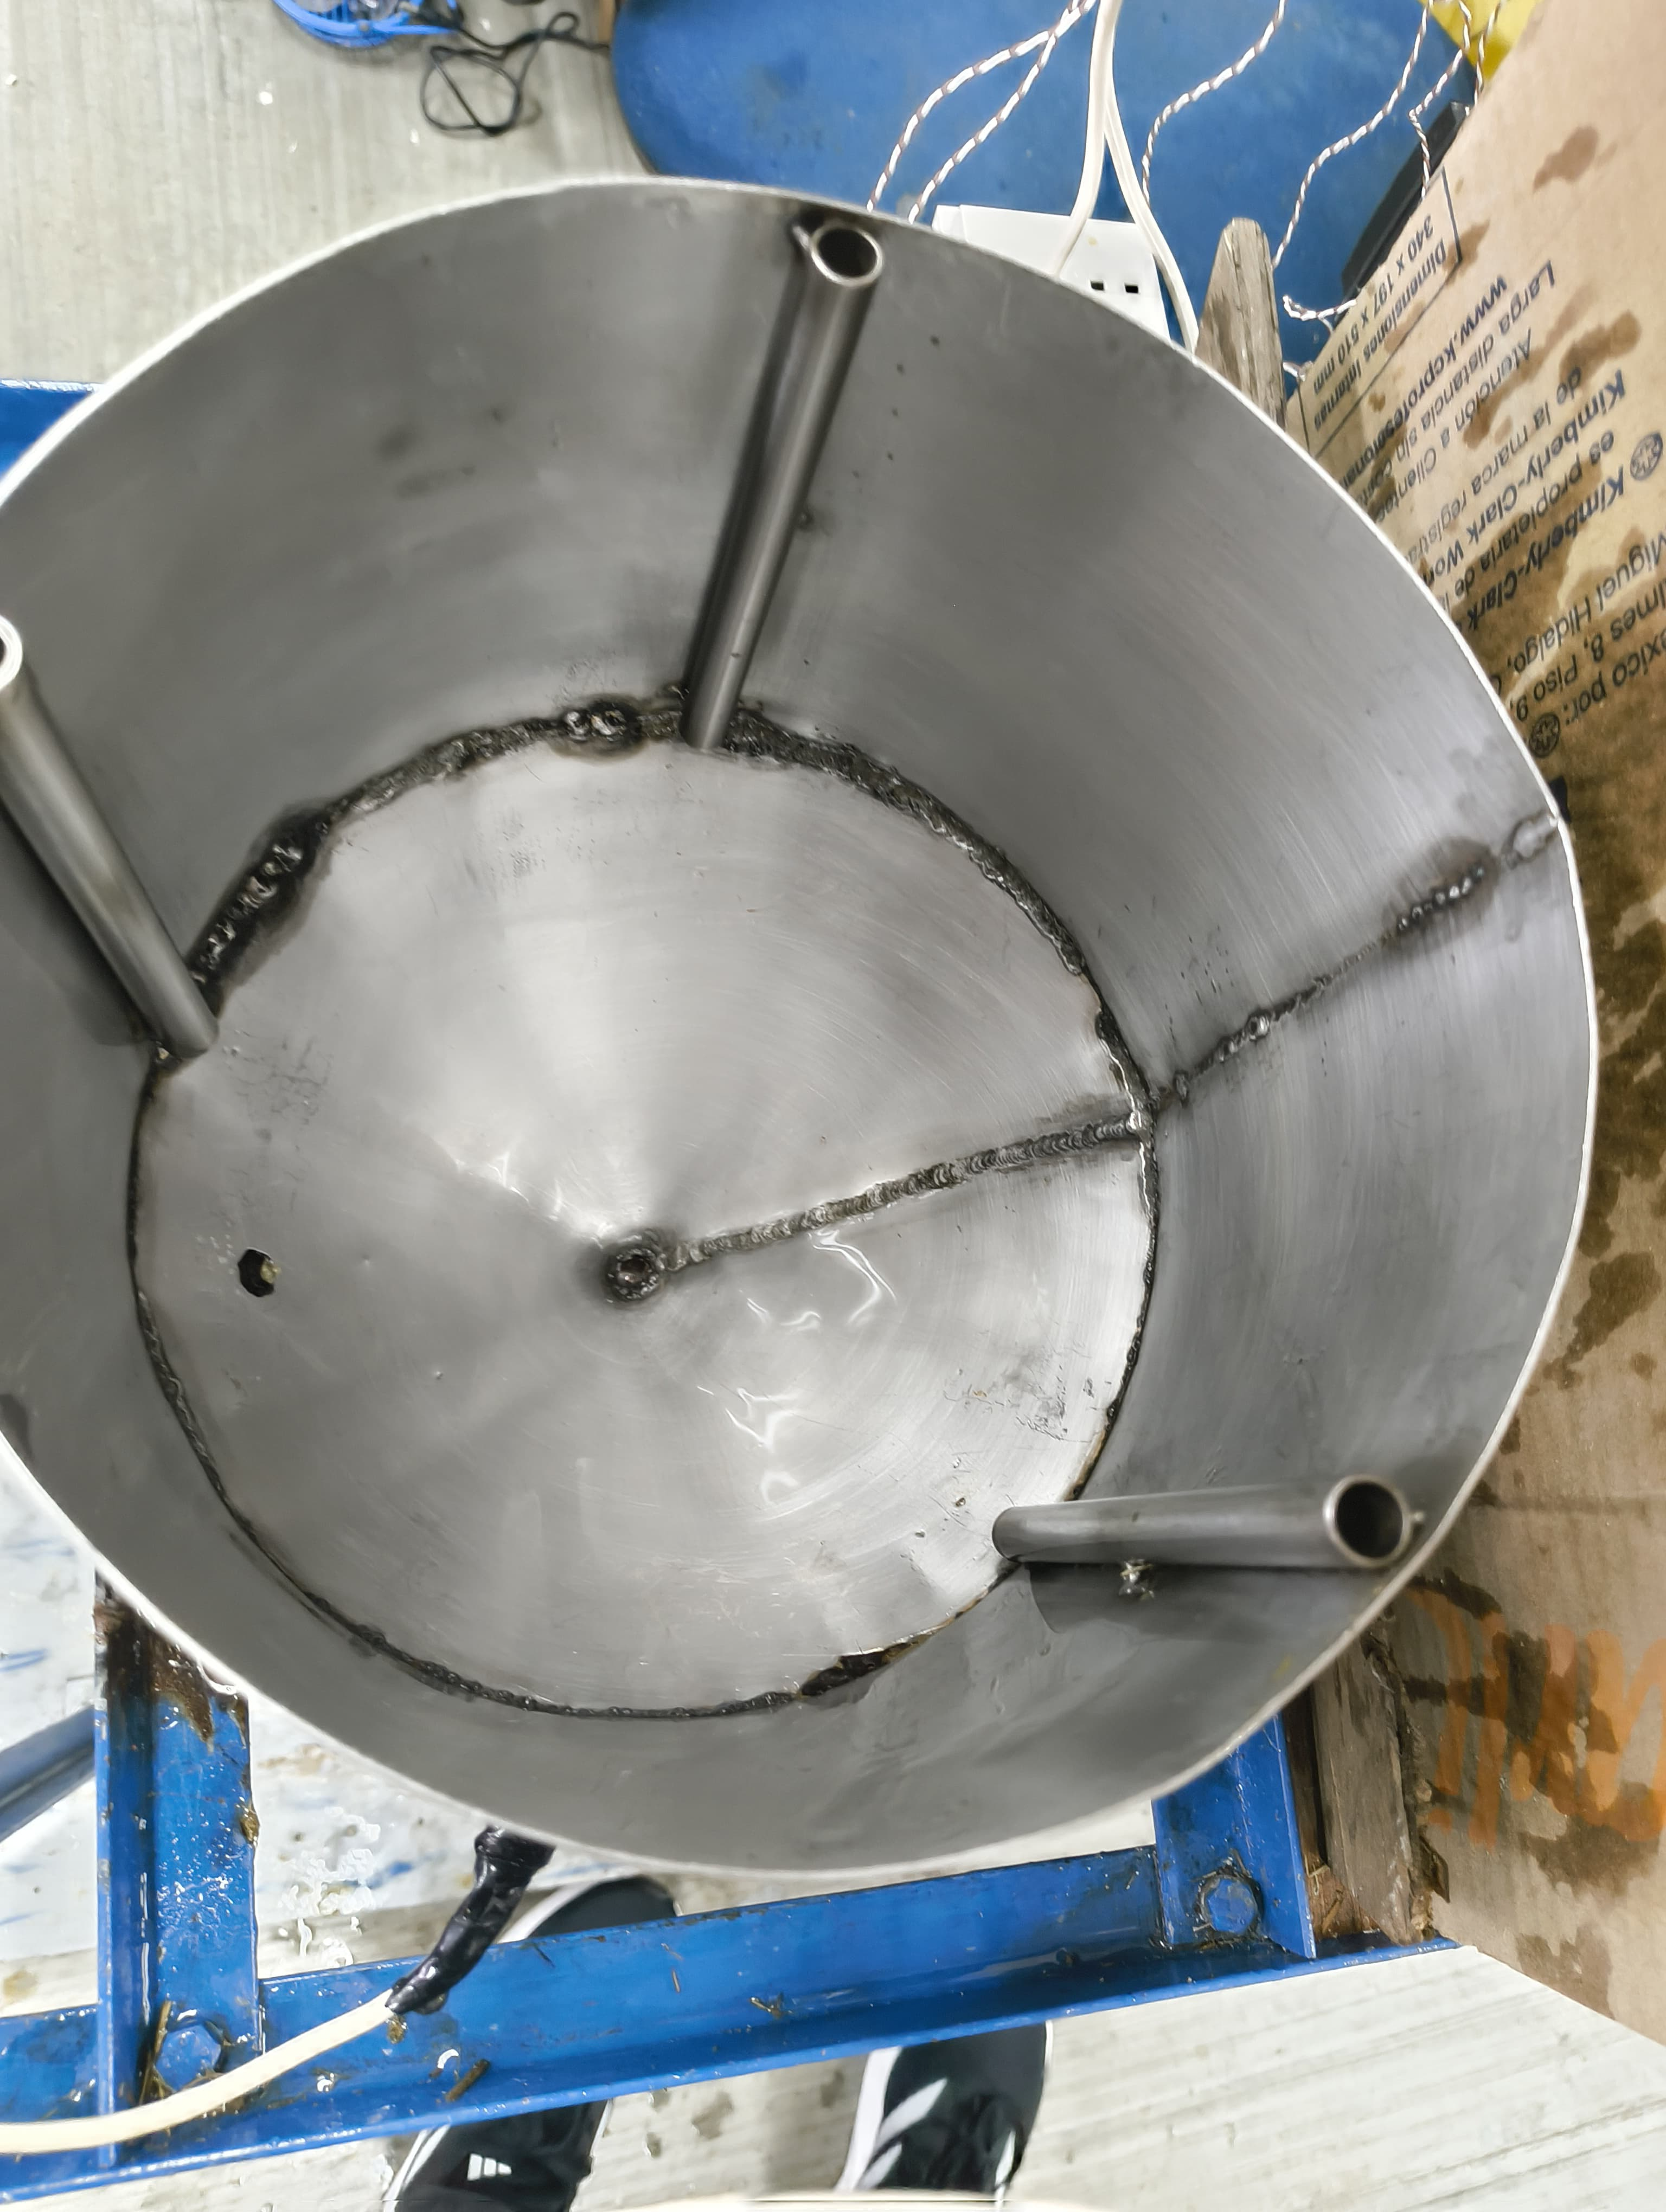
\includegraphics[width=3cm, height=5cm,angle=90]{imagenes/reactor limpio}
				\caption{Reactor tipo batch previamente enjuagado con agua desmineralizada.}
				\label{reactor limpio}
			\end{figure}
			
			\textbf{4.} Se procedió a activar los componentes eléctricos y la resistencia, verificando su correcto funcionamiento. Posteriormente, se instaló el tornillo de sellado en la base del reactor, asegurando su hermeticidad. En el interior del equipo previamente sanitizado se incorporaron el agua desmineralizada y el bagazo de caña en las proporciones establecidas, iniciando así el proceso de tratamiento. 
			
			\textbf{5.} Se incorporó el hidróxido de sodio (NaOH) previamente dosificado al reactor que contiene la mezcla de agua desmineralizada y bagazo de caña,  como se documenta en la Figura \ref{bagazo con hidroxido}.
			
			
			\begin{figure}[H]
				\centering
				\begin{minipage}{0.46\textwidth}
					\centering
					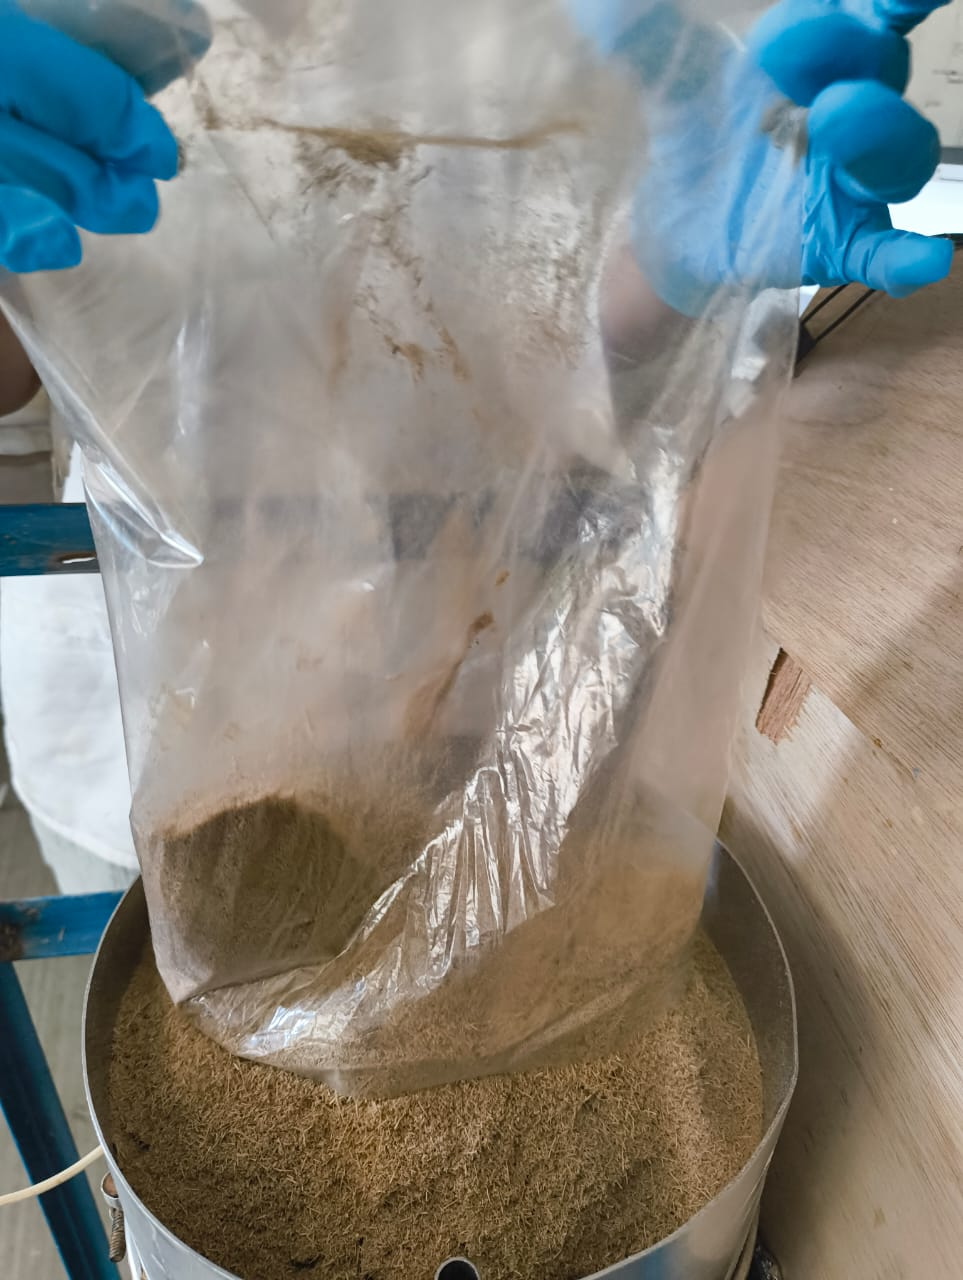
\includegraphics[width=3cm, height=3cm]{imagenes/agua con bagazo}
					\caption{Se agrega el bagazo de caña al reactor con agua desmineralizada.}
					\label{agua con bagazo}
				\end{minipage}
				\hfill
				\begin{minipage}{0.48\textwidth}
					\centering
					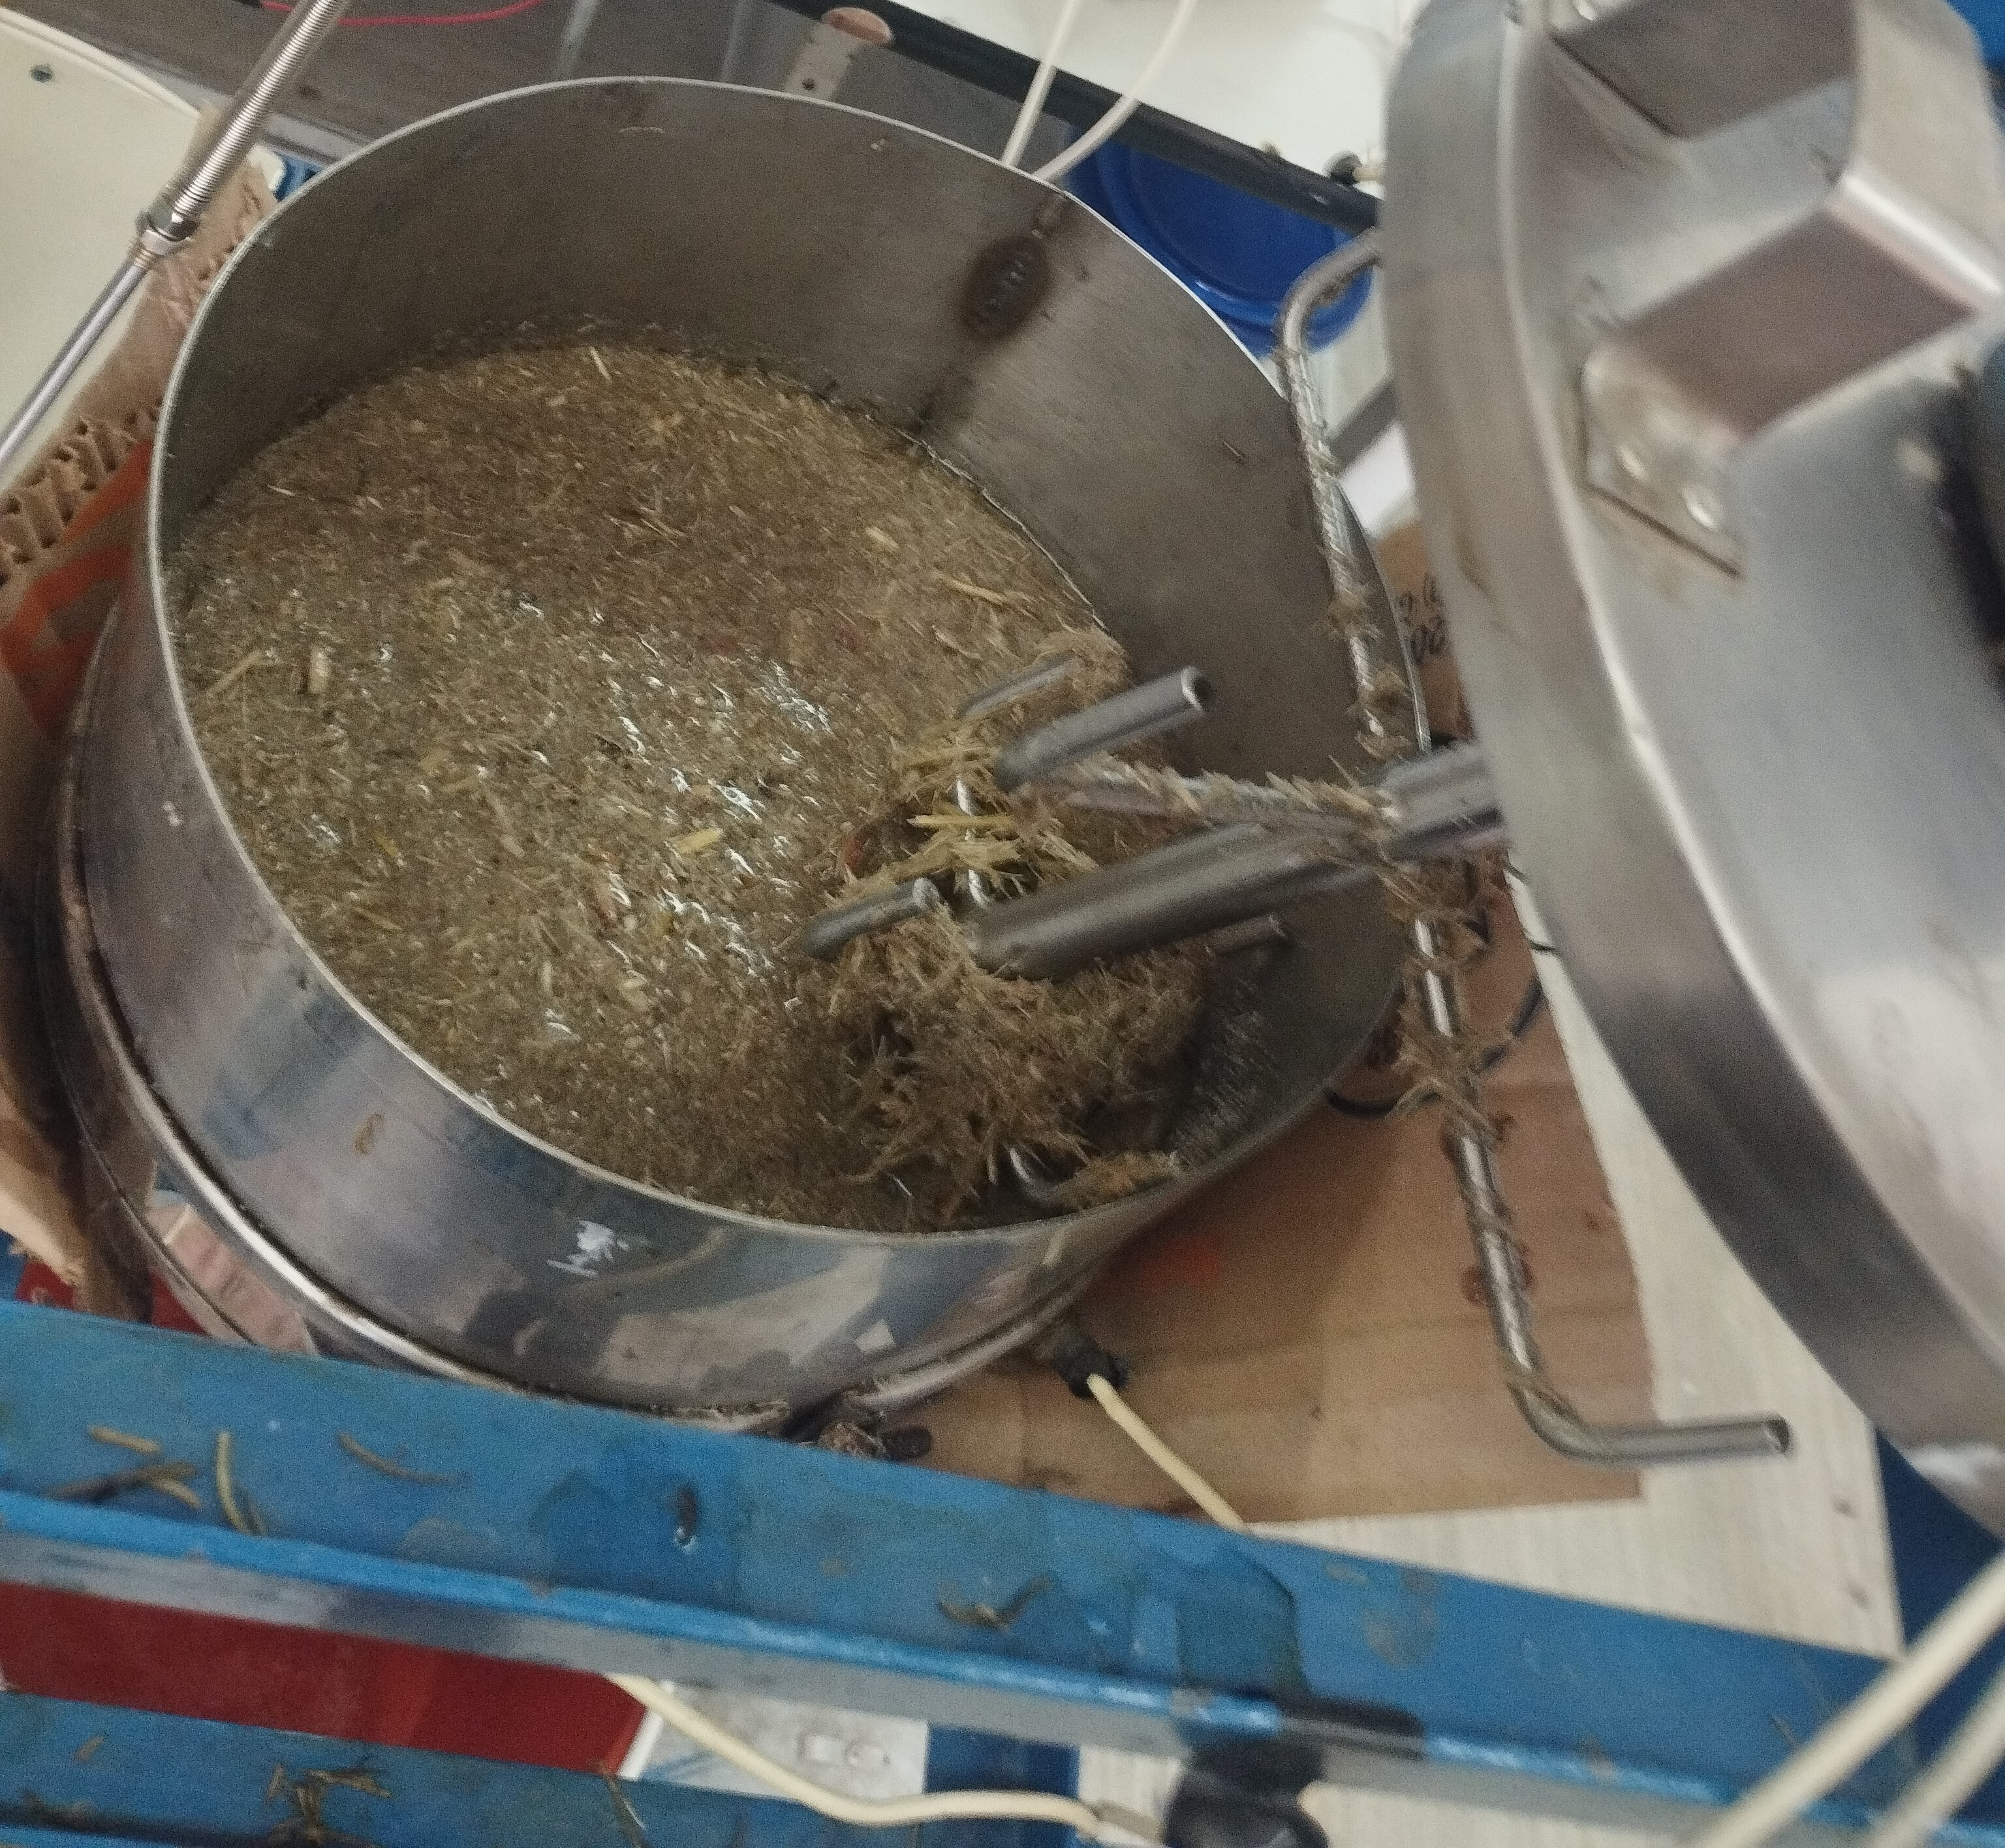
\includegraphics[width=5cm, height=3cm]{imagenes/bagazo con hidroxido1}
					\caption{Se agrega el hidróxido y se mezcla hasta incorporarse.}
					\label{bagazo con hidroxido}
				\end{minipage}
			\end{figure}
			
			
			\textbf{6.} El reactor se selló herméticamente mediante un sistema multicapa compuesto por: algodón como barrera primaria, papel aluminio para aislamiento térmico y cinta aislante/ térmica como sellado secundario, garantizando el cierre completo del sistema como se detalla en la Figura \ref{sellado_bio}.
			
			
			
			\textbf{7.} Finalmente, se activó el sistema de control automatizado (Figura \ref{programa}), para seguir los perfiles programados de temperatura para el interior del reactor y el tiempo de pretratamiento establecidos en el diseño experimental (Figura \ref{Diagrama1}). Este control garantizó las condiciones requeridas para el proceso.
			
			
			\begin{figure}[H]
				\centering
				\begin{minipage}{0.46\textwidth}
					\centering
					\includegraphics[width=\linewidth, height=4cm, keepaspectratio]{imagenes/sellado2}
					\caption{El reactor se sella con ayuda de algodón, papel aluminio y cinta de aislar o cinta térmica.}
					\label{sellado_bio}
				\end{minipage}
				\hfill
				\begin{minipage}{0.48\textwidth}
					\centering
					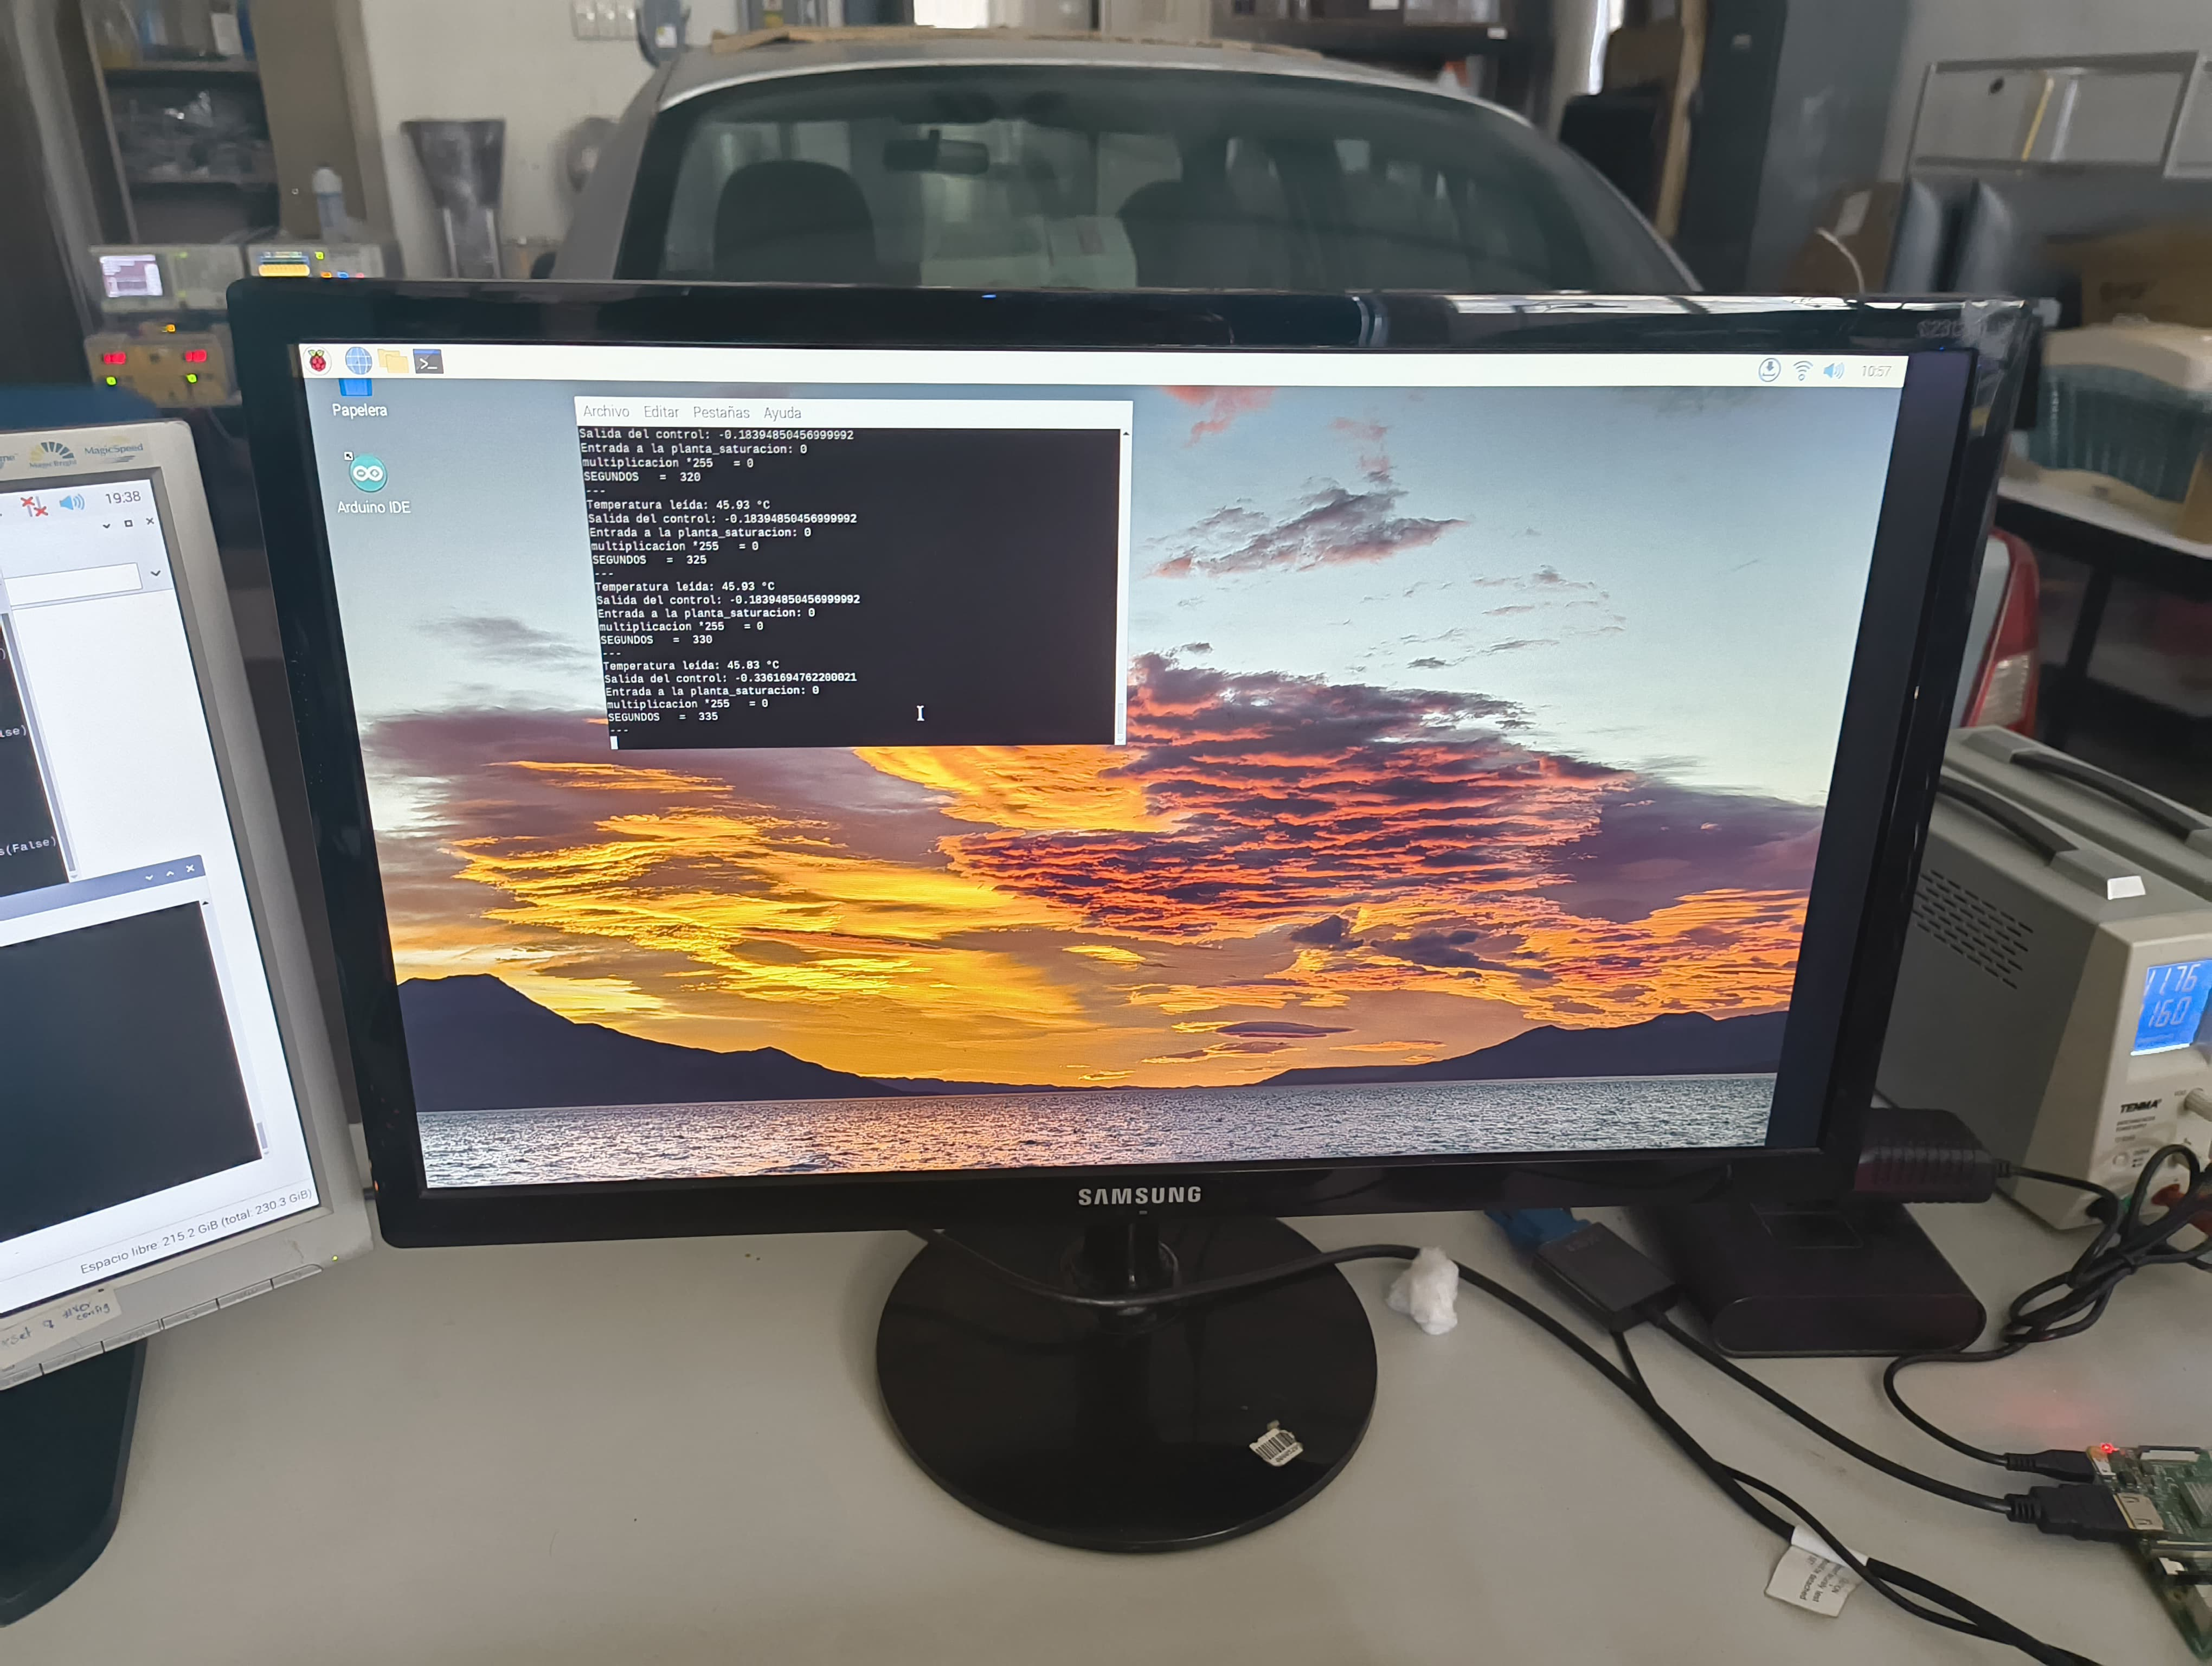
\includegraphics[width=\linewidth, height=4cm, keepaspectratio]{imagenes/programa3}
					\caption{Se muestra el programa en funcionamiento.}
					\label{programa}
				\end{minipage}
			\end{figure}
			
			\textbf{7.} El diseño del control de temperatura para llevar a cabo este pretratamiento de la biomasa está reportado en el anexo \ref{diseño del control de temp}.
			
			%%%%%%%%%%%%%%%%%%%%%%%%%%%%%%%%%%%%%%%%%%%%%%%%%%%%%%%%%%%%%%%%%%%%%%%%%%%%%%%%%%%%%%%%%%%%%%%%%%%%%%%%%%%%%%%%%%%%%%%%%%%%%%%%%%%%%%%%%%%%%%%%%%%%%%%%%%%%%\t
			
			
			
			\subsubsection{Acondicionamiento para el material pretratado}
			
			 \textbf{Materiales}
			\\[0.5em]
		
			\begin{tabular}{p{0.3\textwidth}p{0.3\textwidth}p{0.3\textwidth}}
				$\bullet$ \textit{Agua desmineralizada} & $\bullet$ \textit{ Bagazo de caña Pretratado} & $\bullet$ \textit{Tela delgada}  \\
			
				$\bullet$ \textit{Colador} & $\bullet$ \textit{Cubeta 10 l} & 
			\end{tabular}
			\\[0.5em]
			
			
			\textbf{Procedimiento}
			\\[0.5em] 
			\textbf{1.} Durante el pretratamiento biológico se registraron periódicamente los datos experimentales para garantizar su trazabilidad, y al finalizar el proceso, se almacenó toda la información recopilada. Adicionalmente, se registró el consumo energético mediante la lectura del watímetro (Figura \ref{watimetro}), el cual cuantificó la energía utilizada en kilovatios-hora (kWh) a lo largo del tratamiento.
			
			
			\textbf{2.} Bajo condiciones controladas, se desarmó el sistema, retirando primero los elementos de sellado (aluminio/algodón), luego los componentes electrónicos (sensores termopares tipo k) y finalmente el conjunto tapa-mezclador, dejando la configuración documentada en la Figura \ref{biologico1}.
	
			
					
			\begin{figure}[H]
				\centering
				\begin{minipage}{0.46\textwidth}
					\centering
					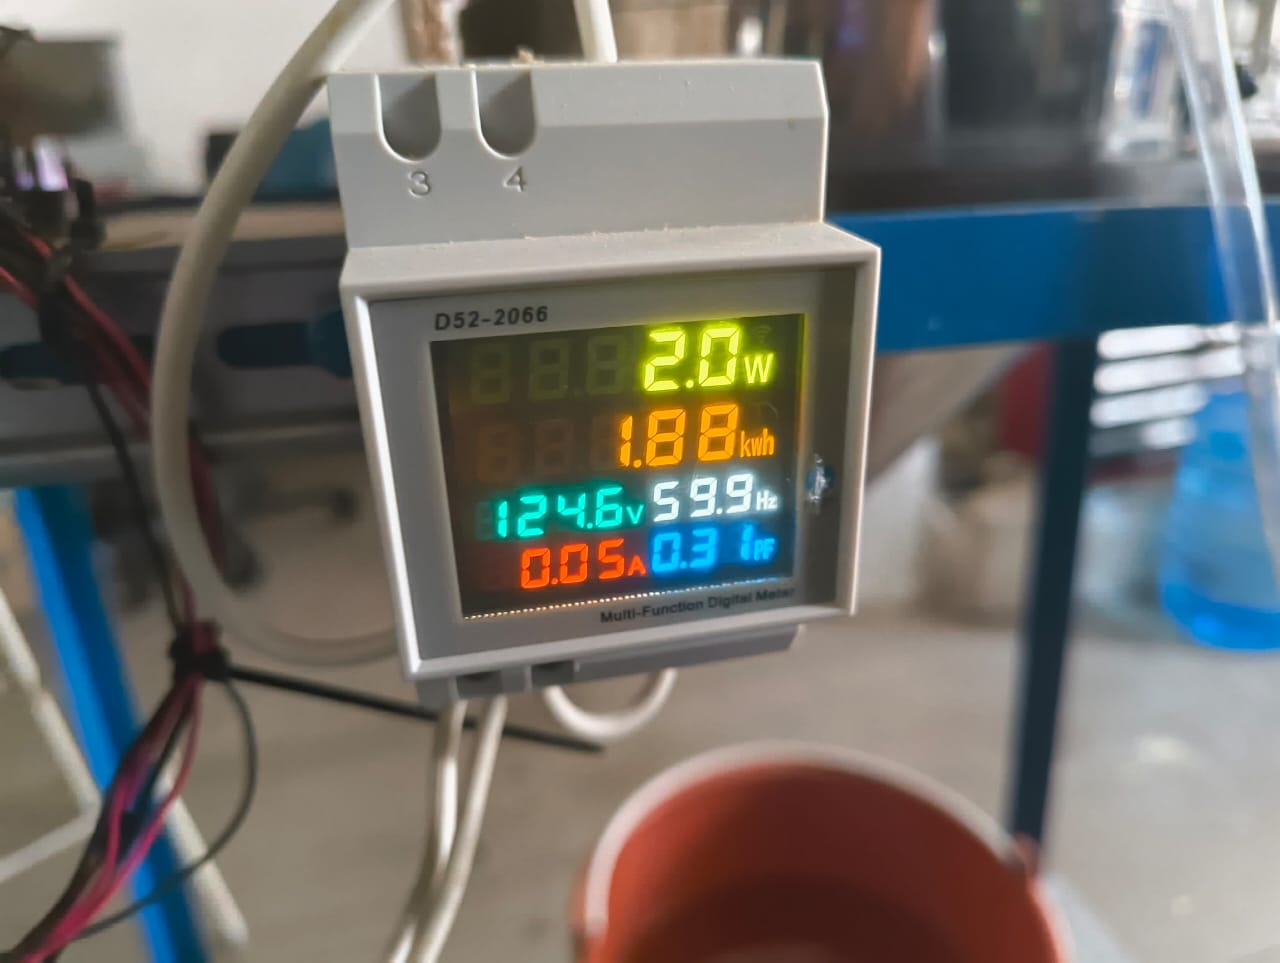
\includegraphics[width=5cm, height=3cm]{imagenes/watimetro} % Cambia "imagen1.jpg" por el nombre de tu archivo
					\caption{Se observa el watimetro que se encuentra en la estructura y mide la energia que entra al convertidor.}
						\label{watimetro}
					\end{minipage}
					\hfill
					\begin{minipage}{0.48\textwidth}
						\centering
						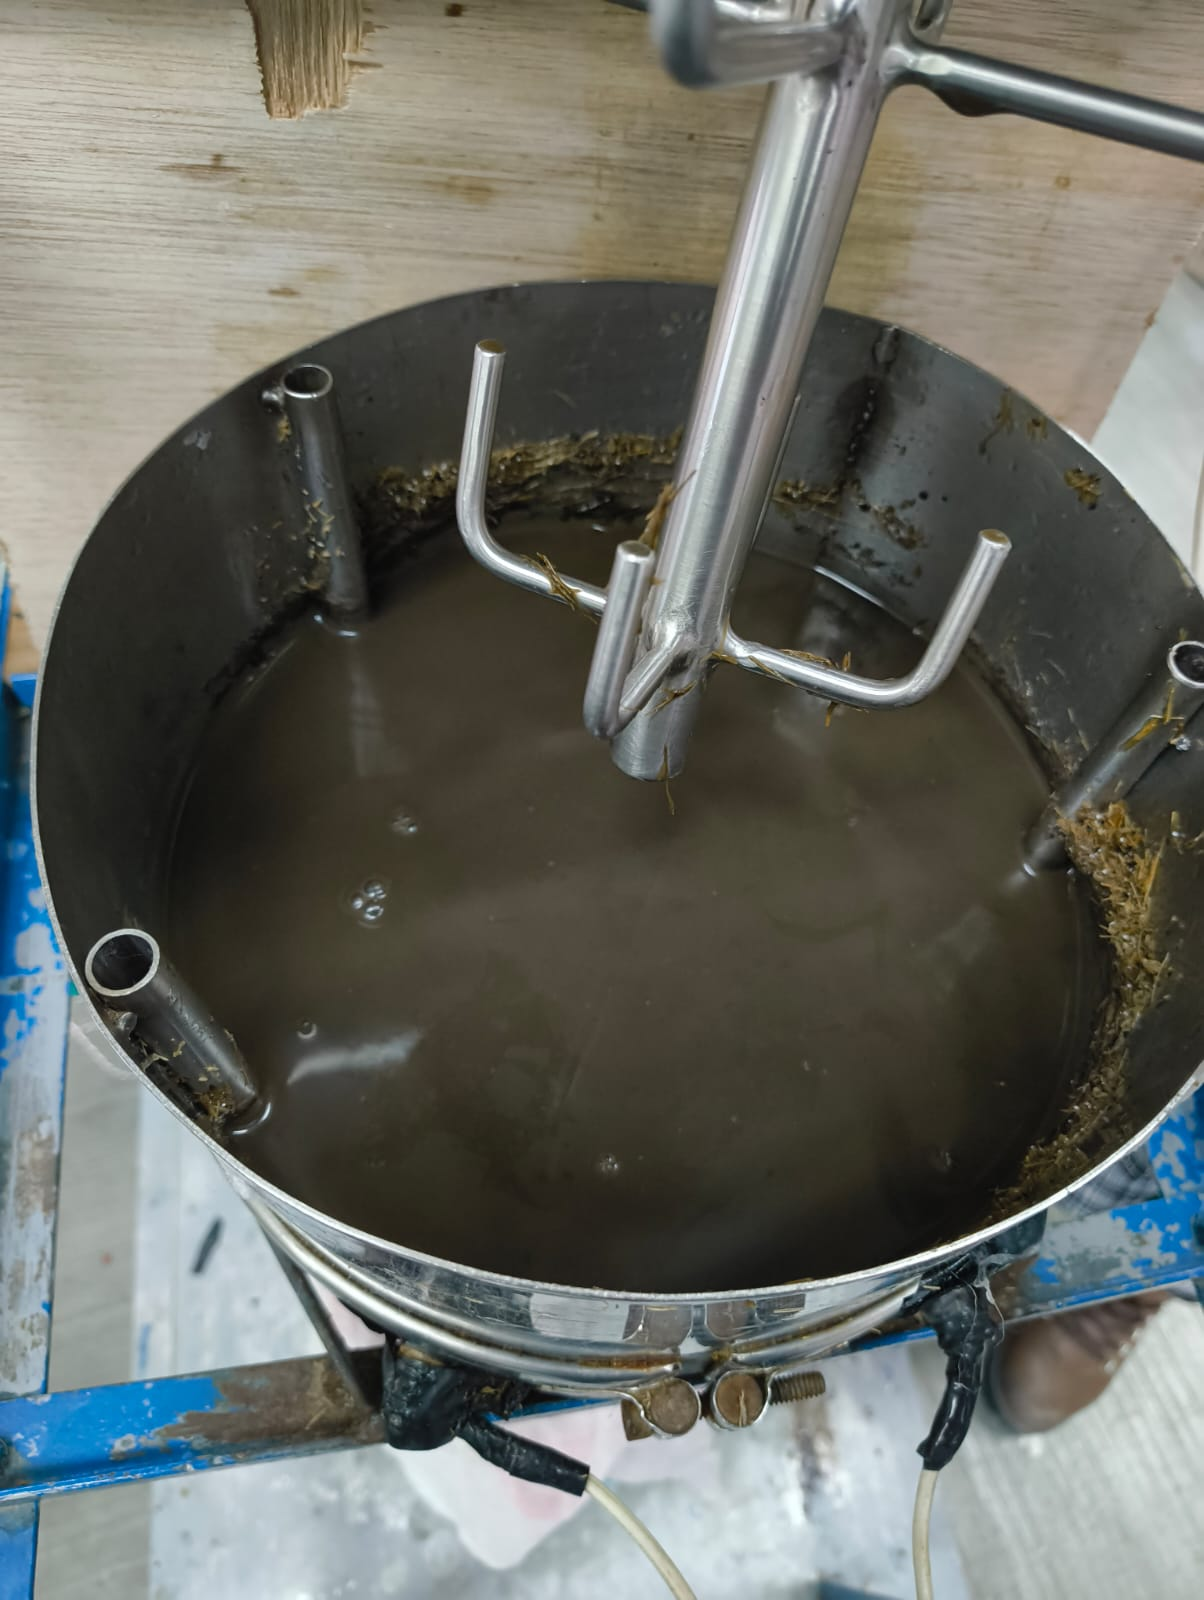
\includegraphics[width=4cm, height=3cm]{imagenes/biologico1} % Cambia "imagen2.jpg" por el nombre de tu archivo
						\caption{Se observa el watimetro que se encuentra en la estructura y mide la energia que entra al convertidor.}
						\label{biologico1}
					\end{minipage}
				\end{figure}
				
			
			\textbf{3.} Para la separación sólido-líquido se implementó un sistema de filtración compuesto por una cubeta de 10 L que integraba una manta filtrante y un colador (Figura \ref{Cubeta con colador y manta para colar el bagazo pretratado.}). En este dispositivo se colocó el bagazo pretratado, permitiendo la retención de la biomasa y el paso del liquido resultante, tal como se documenta en la Figura \ref{Bagazo1}.
 
				\begin{figure}[H]
				\centering
				\begin{minipage}{0.46\textwidth}
					\centering
					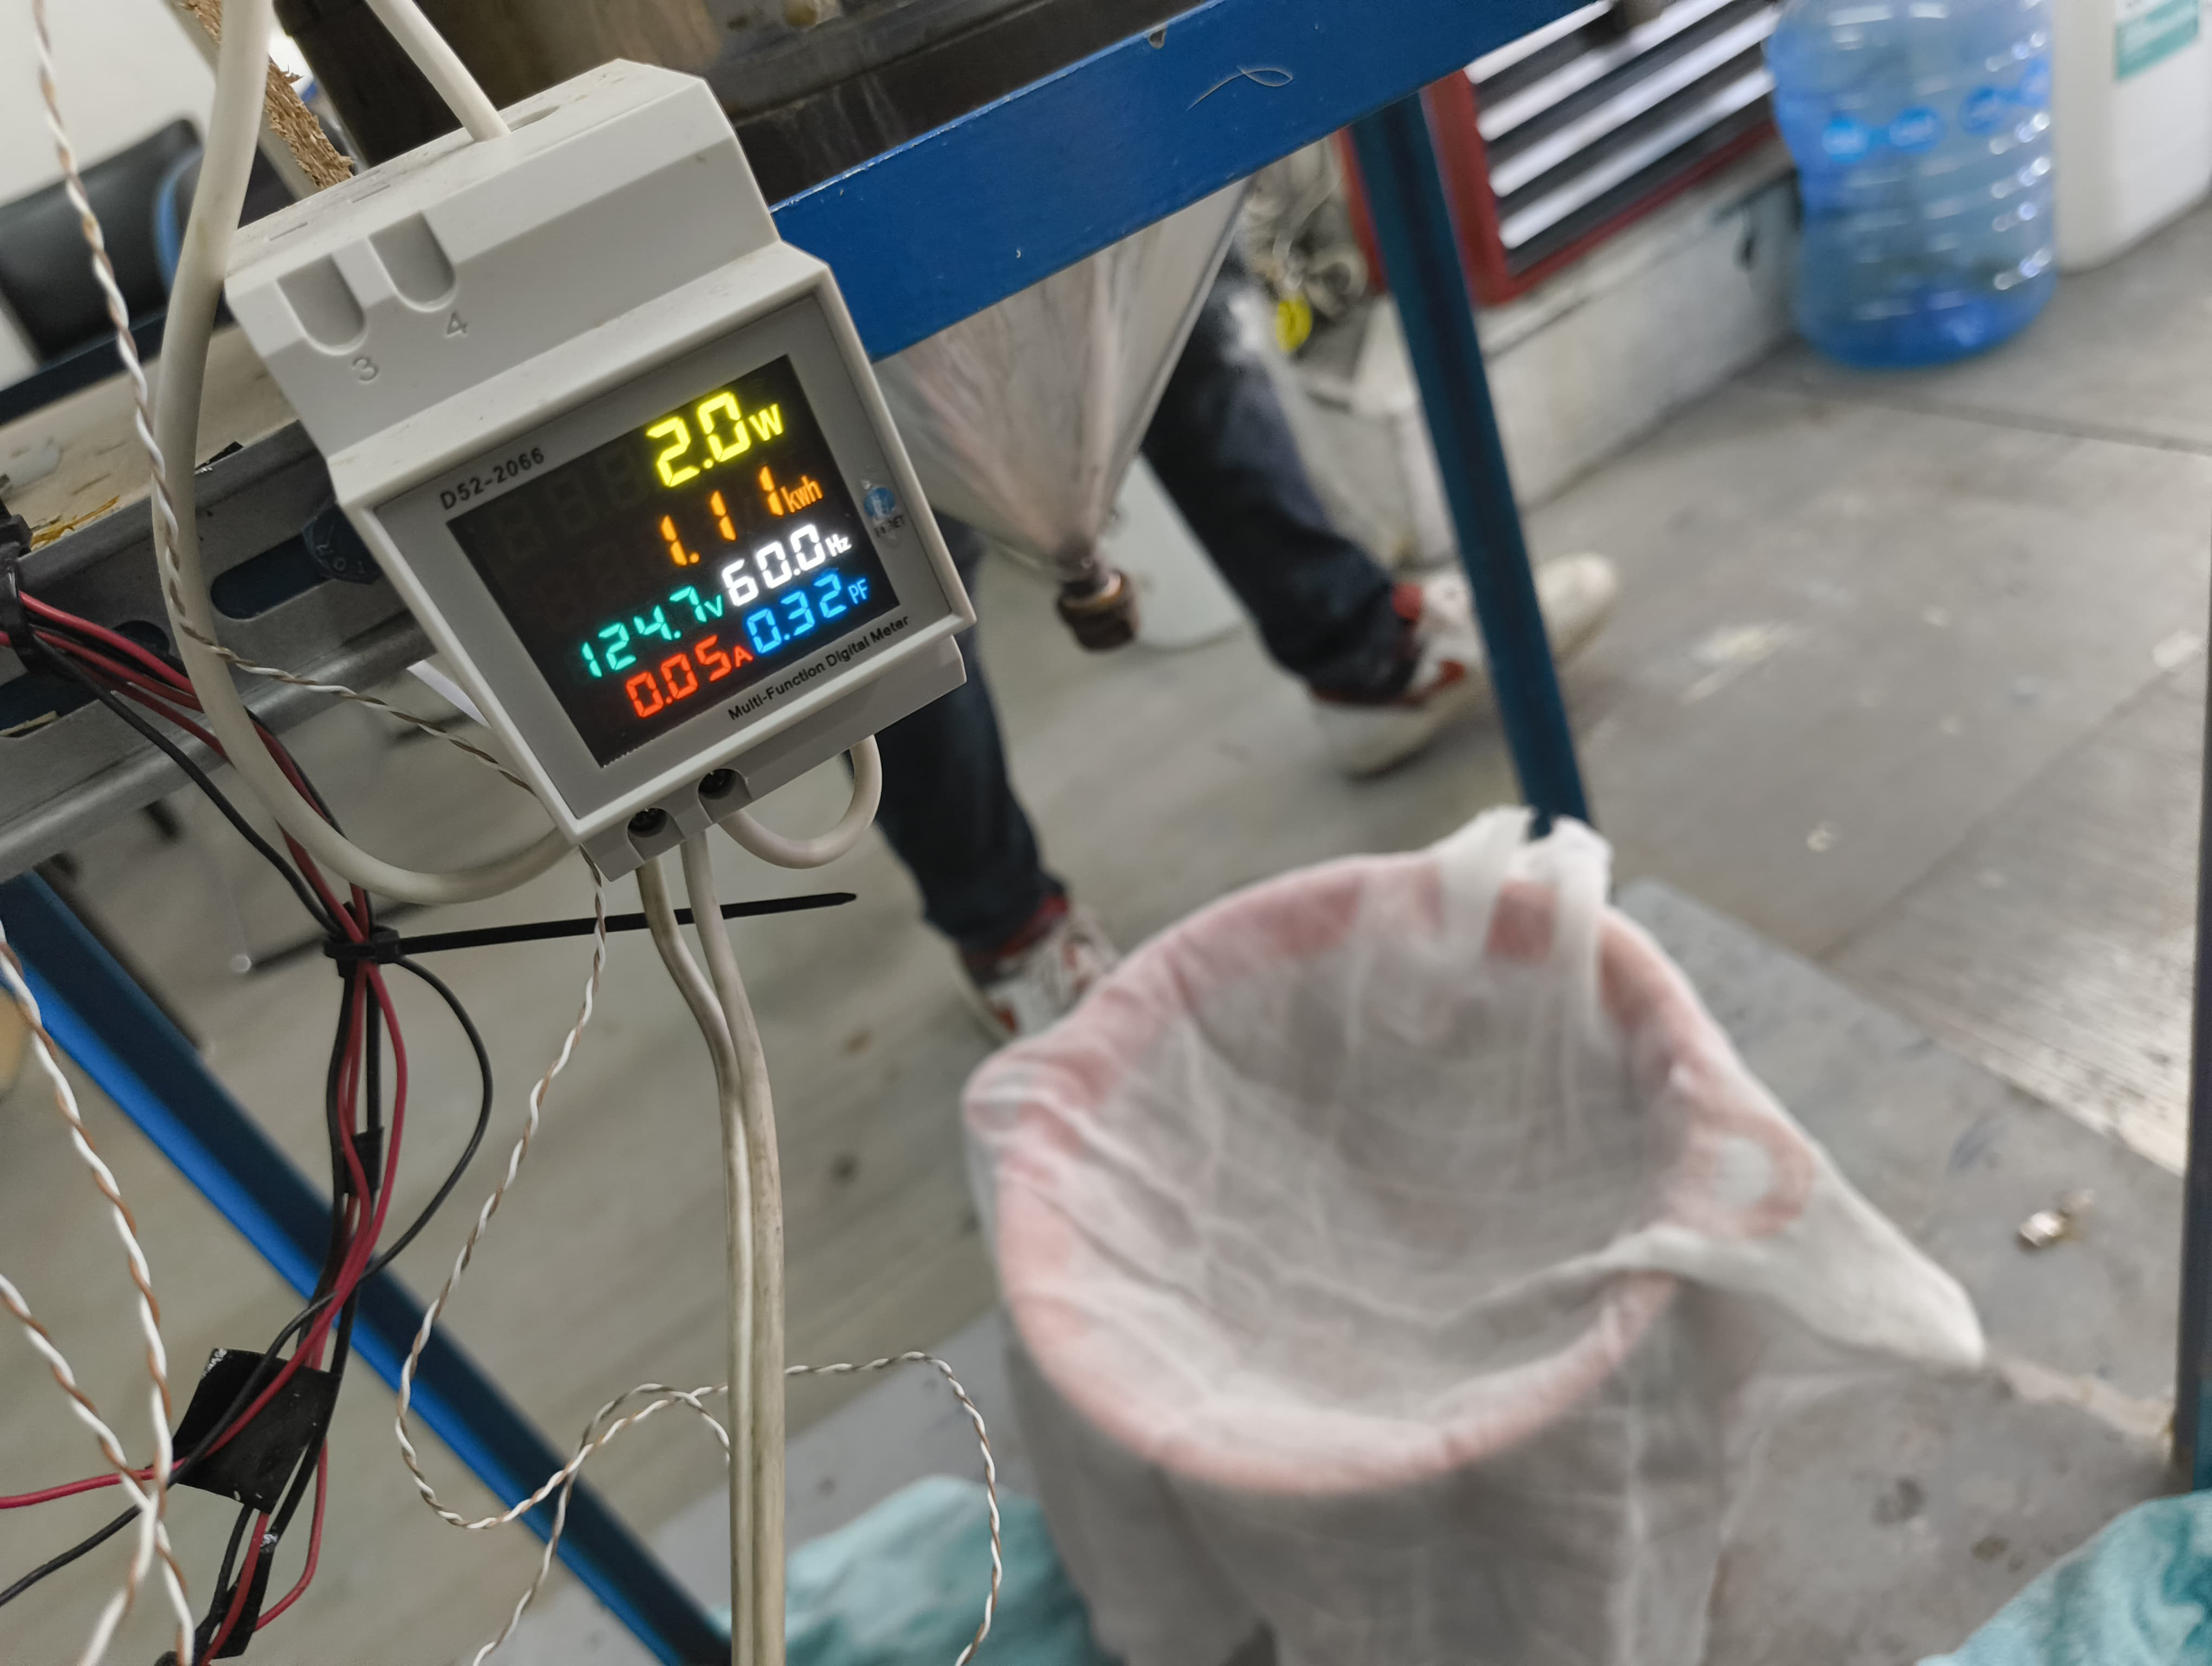
\includegraphics[width=5cm, height=3cm]{imagenes/biologico6} % Cambia "imagen1.jpg" por el nombre de tu archivo
					\caption{Cubeta con colador y manta para colar el bagazo pretratado.}
					\label{Cubeta con colador y manta para colar el bagazo pretratado.}
				\end{minipage}
				\hfill
				\begin{minipage}{0.48\textwidth}
					\centering
					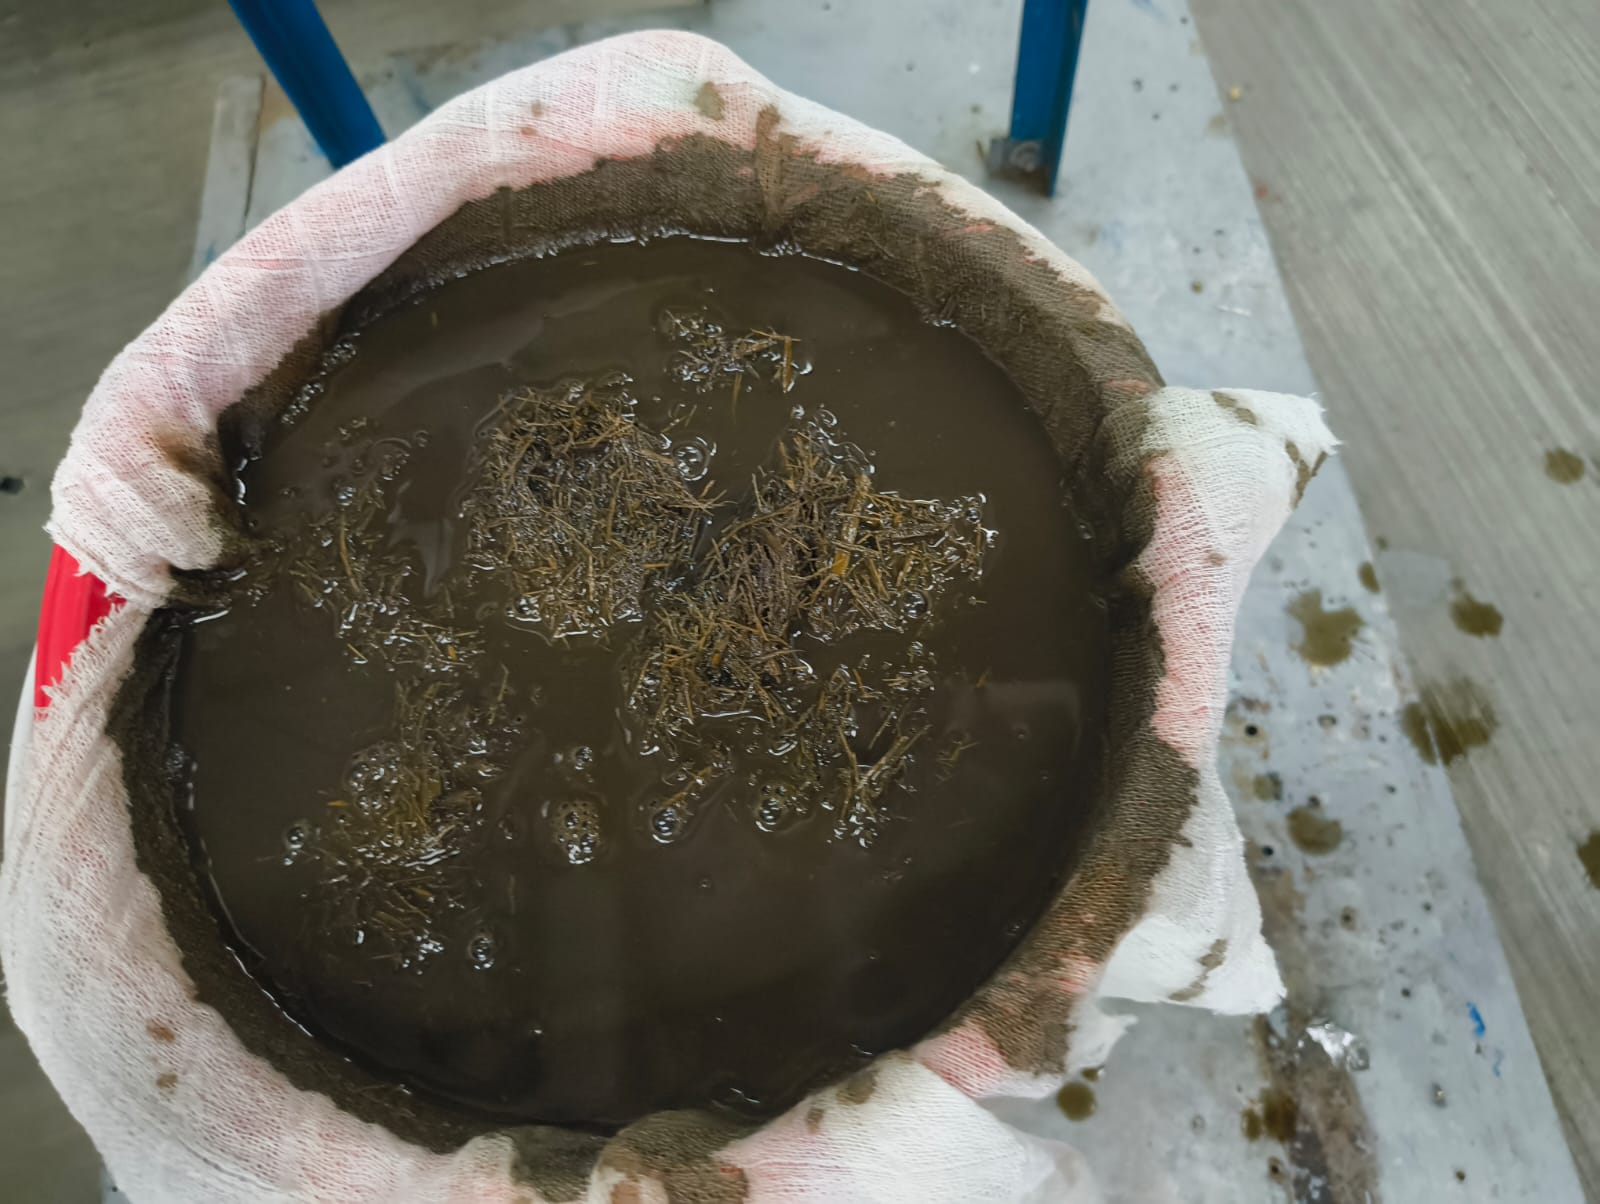
\includegraphics[width=5cm, height=3cm]{imagenes/bagazo_biologico_sacado} % Cambia "imagen2.jpg" por el nombre de tu archivo
					\caption{Bagazo previamente pretratado.}
					\label{Bagazo1}
				\end{minipage}
			\end{figure}
	
	     \textbf{4.} El bagazo pretratado se mantuvo en la cubeta hasta completar el filtrado del agua residual, tras lo cual se sometió a un proceso de lavado con agua adicional para eliminar el máximo posible de humus de lombriz o el hidróxido de sodio respectivamente. Posteriormente, el material se exprimió manualmente para extraer el exceso de líquido y se dejó escurrir, siguiendo el procedimiento ilustrado en la Figura \ref{biologico3}.
	     
	
	\textbf{5.} Para eliminar la humedad residual, el bagazo se extiendió uniformemente en una bandeja y se introdujo en un horno, donde se secó bajo condiciones controladas hasta alcanzar el contenido de humedad deseado, optimizando así el tiempo de proceso como se muestra en la Figura \ref{secado2}. 
	
	
	

	
		\begin{figure}[H]
		\centering
		\begin{minipage}{0.46\textwidth}
			\centering
			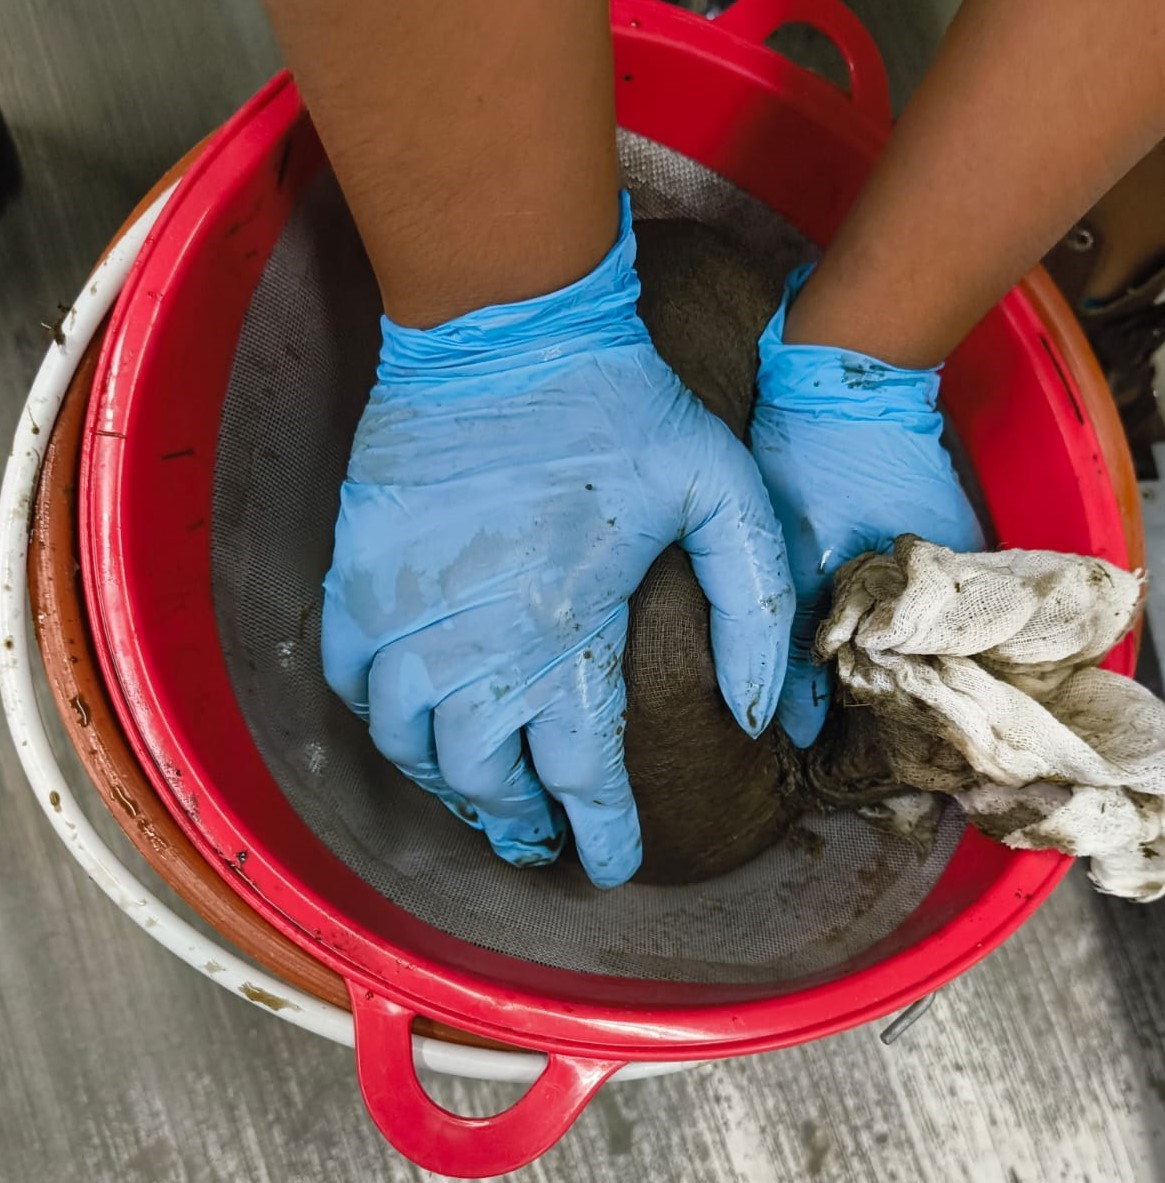
\includegraphics[width=5cm, height=3cm]{imagenes/biologico3} % Cambia "imagen1.jpg" por el nombre de tu archivo
			\caption{En la fotografía muestra como se retira el exceso de agua exprimiendo.}
			\label{biologico3}
		\end{minipage}
		\hfill
		\begin{minipage}{0.48\textwidth}
			\centering
			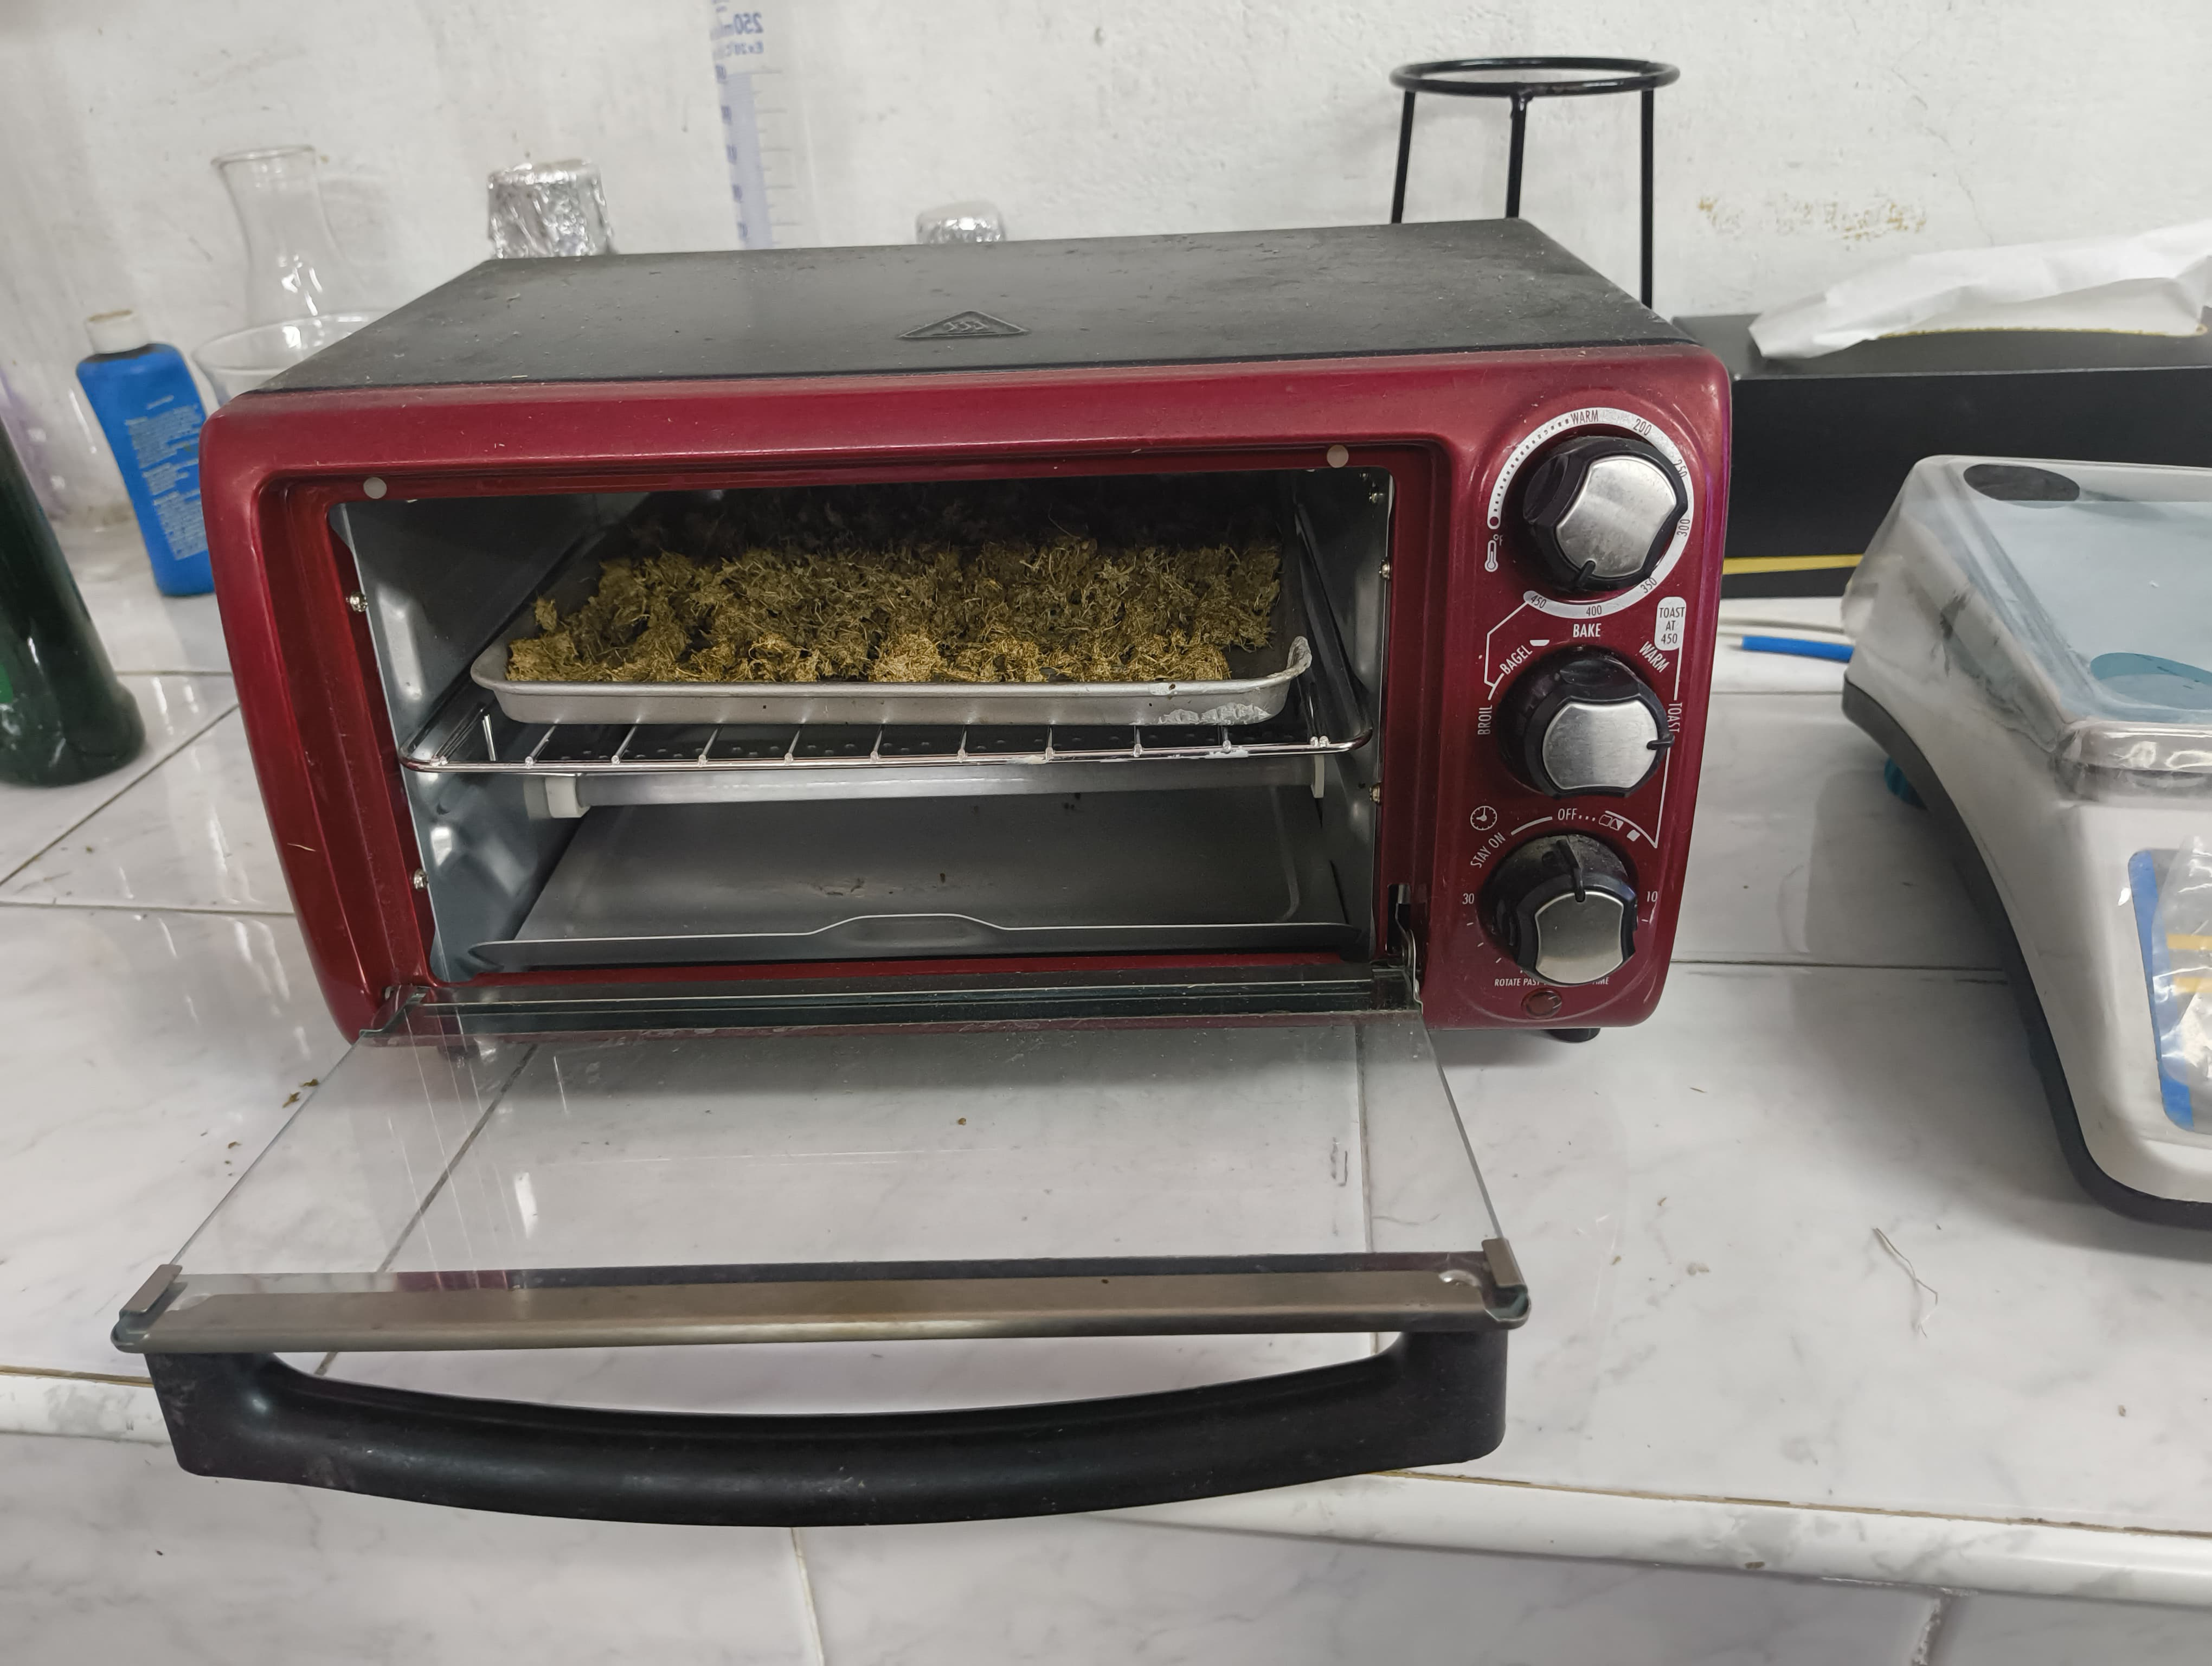
\includegraphics[width=4cm, height=3cm]{imagenes/secado2} % Cambia "imagen2.jpg" por el nombre de tu archivo
			\caption{El bagazo es secado en un horno.}
			\label{secado2}
		\end{minipage}
	\end{figure}
	
	
	
		\textbf{6.} Tras el secado inicial, el bagazo se colocó nuevamente en el colador para someterlo a un segundo enjuague con agua desmineralizada, asegurando la eliminación de residuos solubles (humus de lombriz o hidróxido de sodio), proceso que se documenta en la Figura \ref{enjuagado}.
		
	
		
	  \textbf{7.}Tras el escurrido manual, el material se sometió a secado pasivo en condiciones ambientales (25 ± 2 °C, humedad relativa menor a 60\%) hasta obtener peso constante, verificando la eliminación completa de humedad según se especifica en la Figura \ref{biologico4}.
	
	
		\begin{figure}[H]
		\centering
		\begin{minipage}{0.46\textwidth}
			\centering
			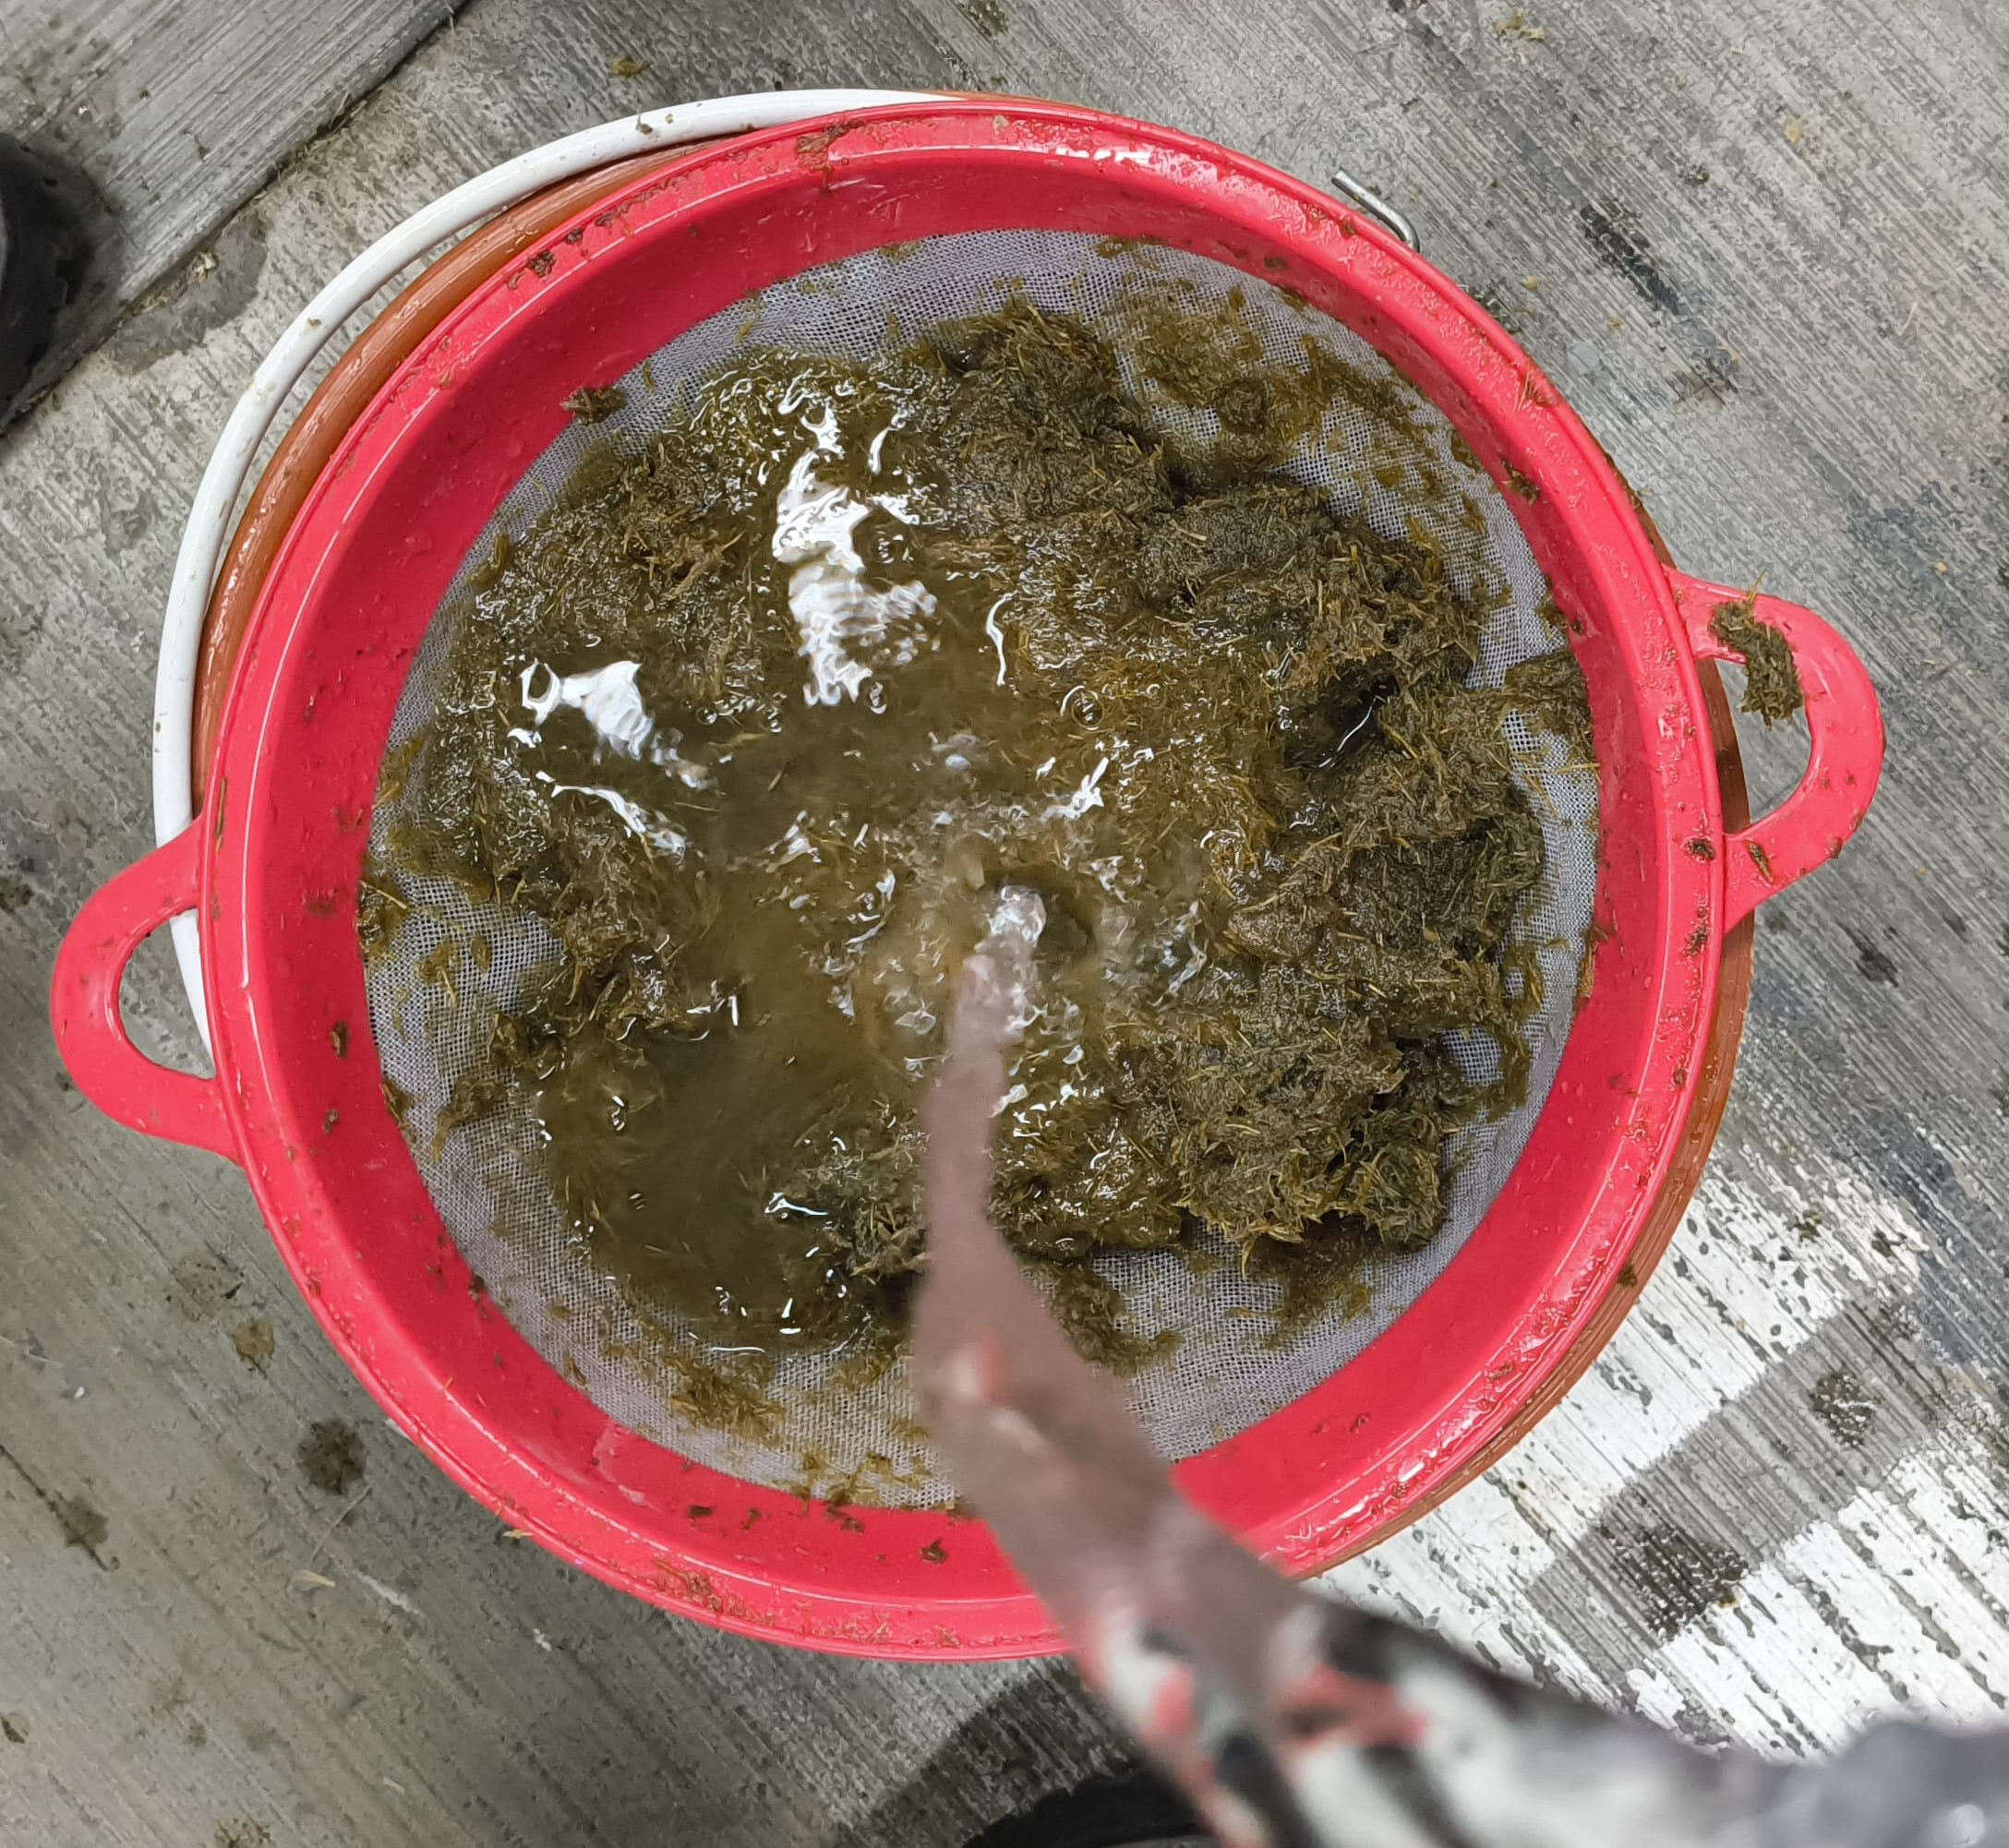
\includegraphics[width=5cm, height=3cm]{imagenes/enjuagado} % Cambia "imagen1.jpg" por el nombre de tu archivo
			\caption{En la fotografía muestra el bagazo después de filtrar el agua.}
			\label{enjuagado}
		\end{minipage}
		\hfill
		\begin{minipage}{0.48\textwidth}
			\centering
			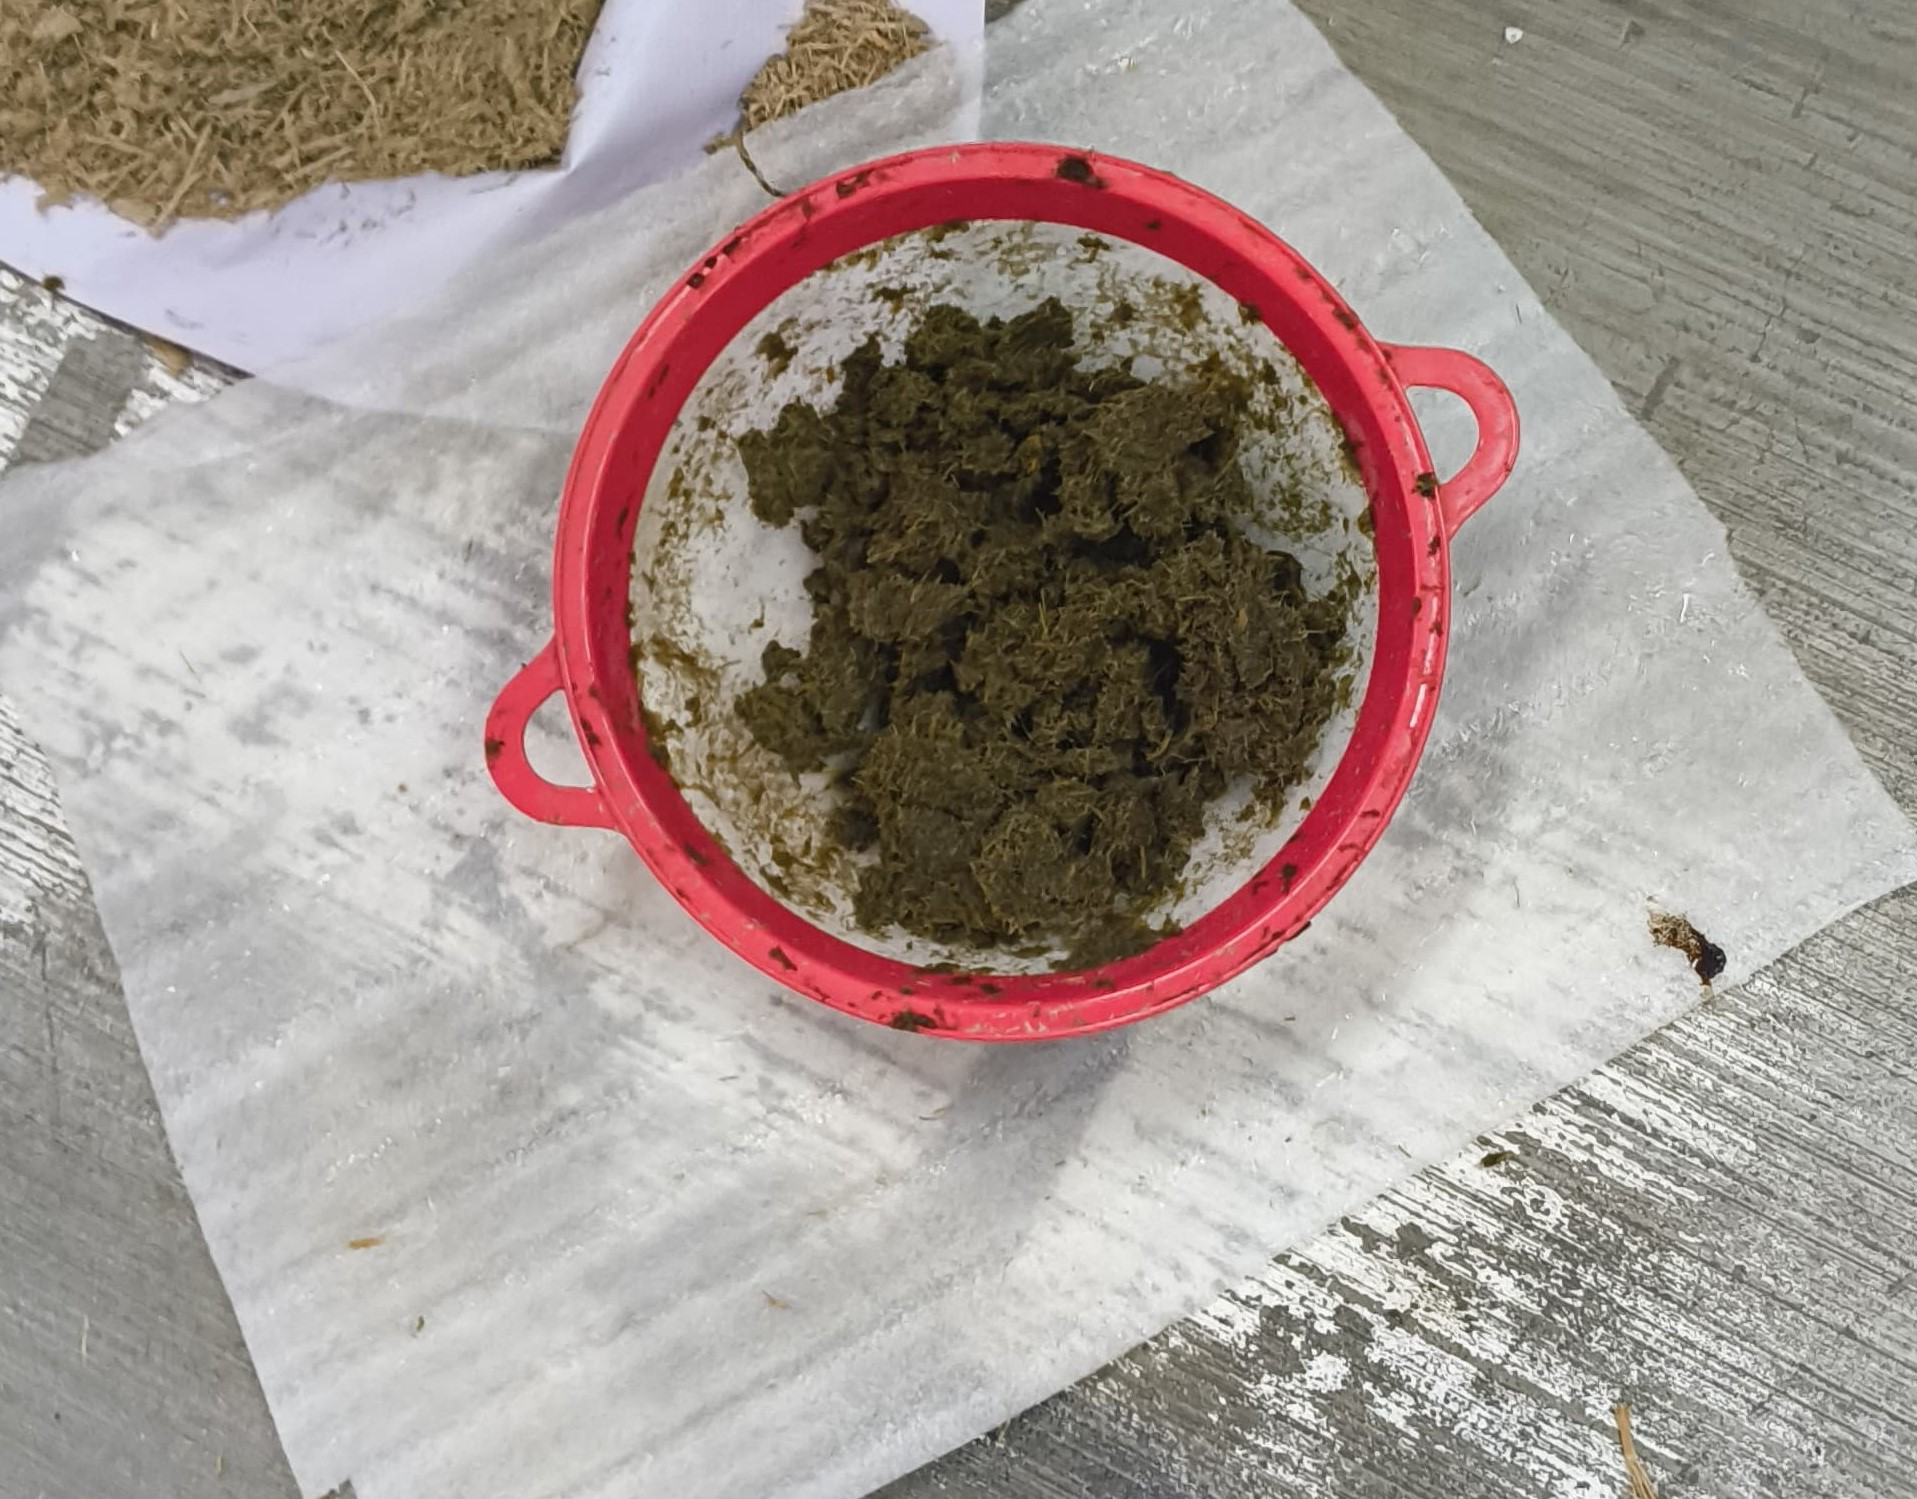
\includegraphics[width=4cm, height=3cm]{imagenes/secado6} % Cambia "imagen2.jpg" por el nombre de tu archivo
			\caption{El bagazo se coloca en un plástico para retirar el agua y la humedad.}
			\label{biologico4}
		\end{minipage}
	\end{figure}
	
	
	
	
	
	 \textbf{8.} Una vez completado el secado, el bagazo se almacenó en bolsas herméticas para prevenir la absorción de humedad ambiental, garantizando así las condiciones óptimas para su uso en los posteriores procesos de la SSF, tal como se muestra en la Figura \ref{biologico4}. Posteriormente el reactor tipo batch fue lavado con agua desmineralizada. \\[0.5em]
	
	\textbf{9.} En el anexo \ref{diseño del control de temp} se reporta el diseño del control de temperatura para este pretratamiento.
	

			
				\subsubsection{Hidrólisis y fermentación en etapas simultaneas}
				
			Para la SSF se consideraron los datos del apartado del diseño factorial, a continuación se presenta la lista de materiales y el procedimiento para la producción de bietanol 2G.
			\\
					 \textbf{Compuestos} \\[0.5em]
					 
				\begin{tabular}{p{0.3\textwidth}p{0.3\textwidth}p{0.3\textwidth}}	 
					 	 	$\bullet$ \textit{Agua desmineralizada} & $\bullet$ \textit{Enzimas Cellic Ctec 2}  & $\bullet$ \textit{Levadura activa} \\
					 $\bullet$ \textit{Ácido Cítrico} & $\bullet$ \textit{Bagazo de caña Pretratado} & \\
					
					\end{tabular}
					 
					 
					 	\textbf{Materiales} 
					 
					 \begin{tabular}{p{0.3\textwidth}p{0.3\textwidth}p{0.3\textwidth}}
					 $\bullet$ \textit{Cinta de teflón} & $\bullet$ \textit{Algodón } & $\bullet$ \textit{ Papel aluminio} \\
					 	$\bullet$ \textit{Cinta térmica}  & $\bullet$ \textit{Vaso de precipitado} &
					 \end{tabular}
					 \\[0.5em]
					 
					 
					 
		  \textbf{Procedimiento}
					\\[0.5em]	 
		 \textbf{1.}  El reactor tipo batch, previamente lavado, fue desinfectado con agua desmineralizada y se procedió a sellar herméticamente su base para garantizar condiciones estériles antes de iniciar el proceso, evitando así cualquier contaminación externa que pueda afectar la reacción.\\[0.5em]

		 	
		 \textbf{2.} Cada reactivo (ácido cítrico, levadura activa) se pesó individualmente usando una báscula digital calibrada y un vaso de precipitado estéril, mientras que el agua se midió volumétricamente, ajustando las cantidades según los parámetros establecidos en el diseño de experimentos para garantizar la reproducibilidad del proceso y la trazabilidad de los datos. Ver Figura\ref{pesado2}.
		 
	
		 
		 \begin{figure}[H]
		 	\centering
		 	\begin{minipage}{0.46\textwidth}
		 		\centering
		 		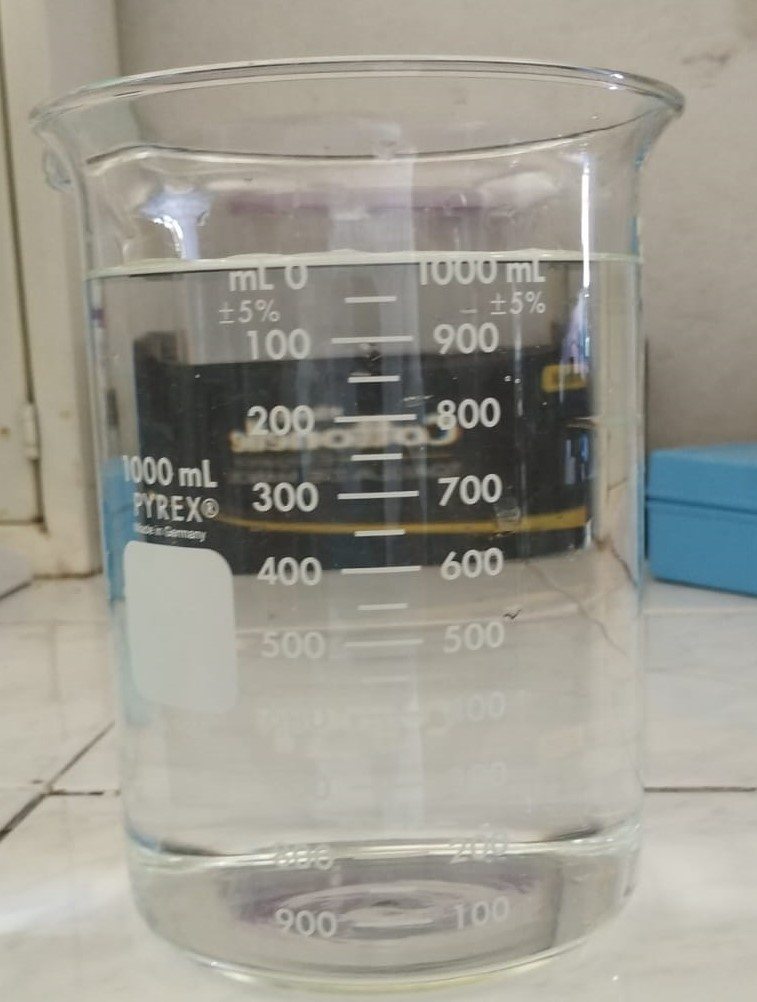
\includegraphics[width=3cm, height=3cm]{imagenes/agua} % Cambia "imagen1.jpg" por el nombre de tu archivo
		 		\caption{ Agua desmineralizada que ayudara a limpiar el reactor.}
		 		\label{agua}
		 	\end{minipage}
		 	\hfill
		 	\begin{minipage}{0.48\textwidth}
		 		\centering
		 		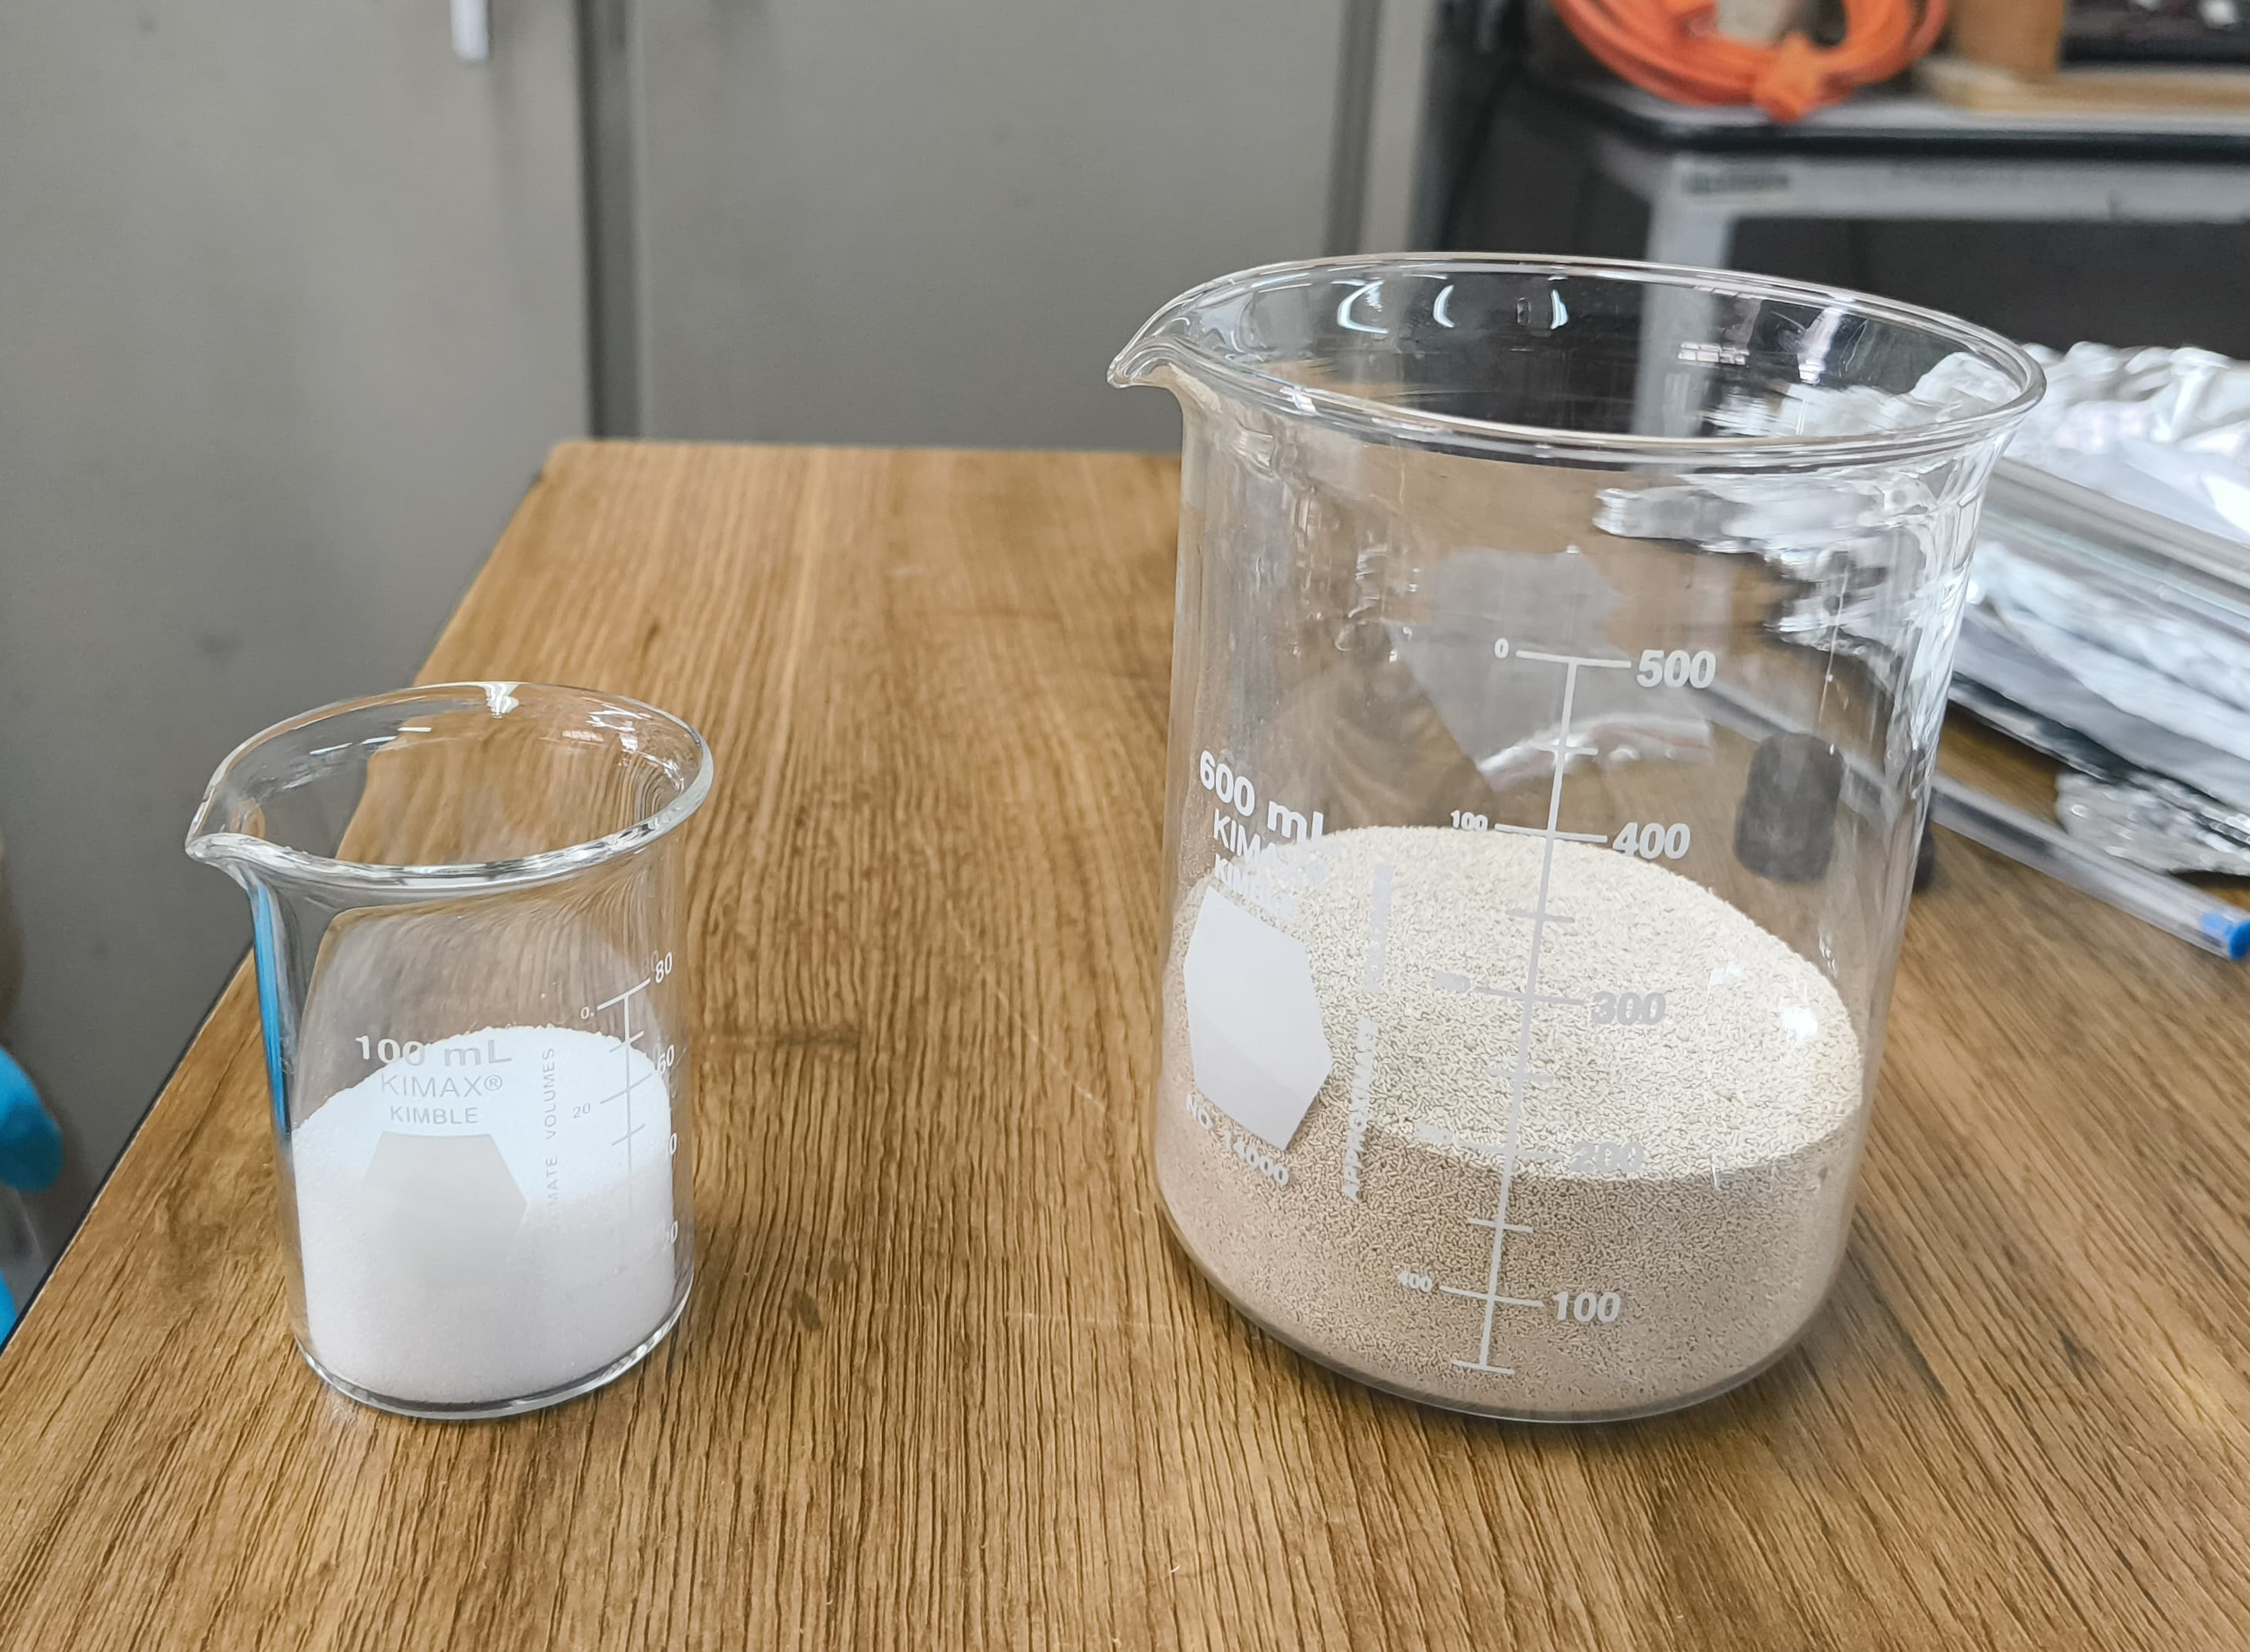
\includegraphics[width=4cm, height=3cm]{imagenes/levadura y acido citrico} % Cambia "imagen2.jpg" por el nombre de tu archivo
		 		\caption{Levadura y ácido cítrico.}
		 		\label{pesado2}
		 	\end{minipage}
		 \end{figure}
		 
		 
	     \textbf{3.} En el interior del reactor tipo batch se depositaron el agua desmineralizada y el bagazo de caña previamente pretratado, siguiendo las proporciones establecidas en el protocolo experimental (como se ilustra en la Figura \ref{ hidrolisis}), asegurando una distribución homogénea de los componentes que garantizara las condiciones requeridas para la reacción.
	     	
	     \textbf{4.} Al reactor tipo batch conteniendo el bagazo de caña pretratado y el agua desmineralizada se le adicionó la levadura activa previamente pesada (ver Figura \ref{hidrolisis4}), la cual se mezcló homogéneamente hasta lograr su completa incorporación al medio de reacción. 
	     
	    
	     
	      
	     \begin{figure}[H]
	     	\centering
	     	\begin{minipage}{0.46\textwidth}
	     		\centering
	     		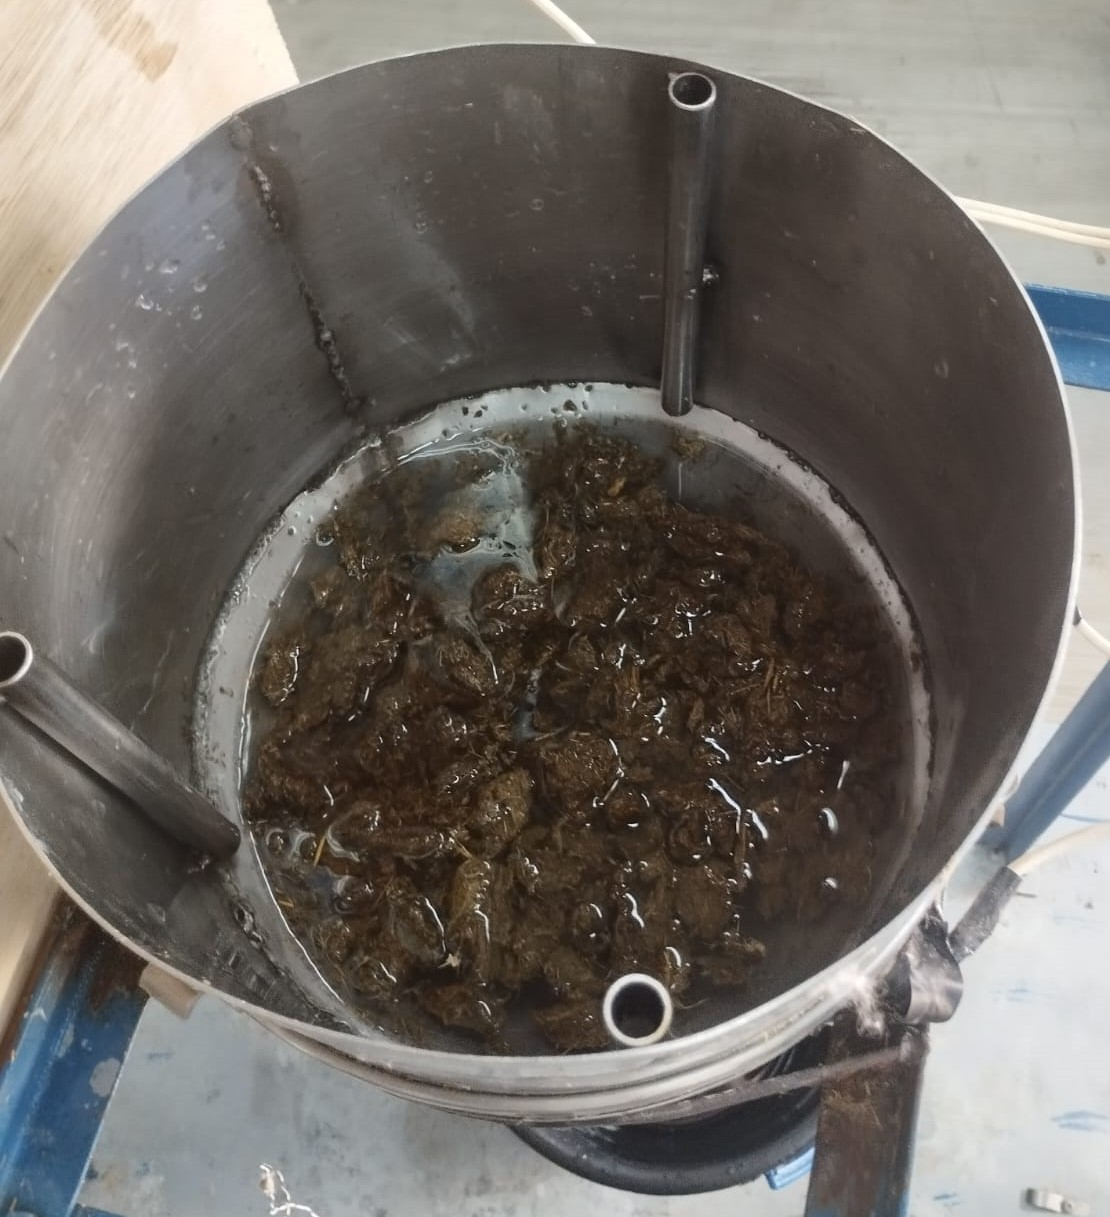
\includegraphics[width=3cm, height=3cm]{imagenes/hidrolisis1} % Cambia "imagen1.jpg" por el nombre de tu archivo
	     		\caption{ Reactor con bagazo previamente pretratado.}
	     		\label{ hidrolisis}
	     	\end{minipage}
	     	\hfill
	     	\begin{minipage}{0.48\textwidth}
	     		\centering
	     		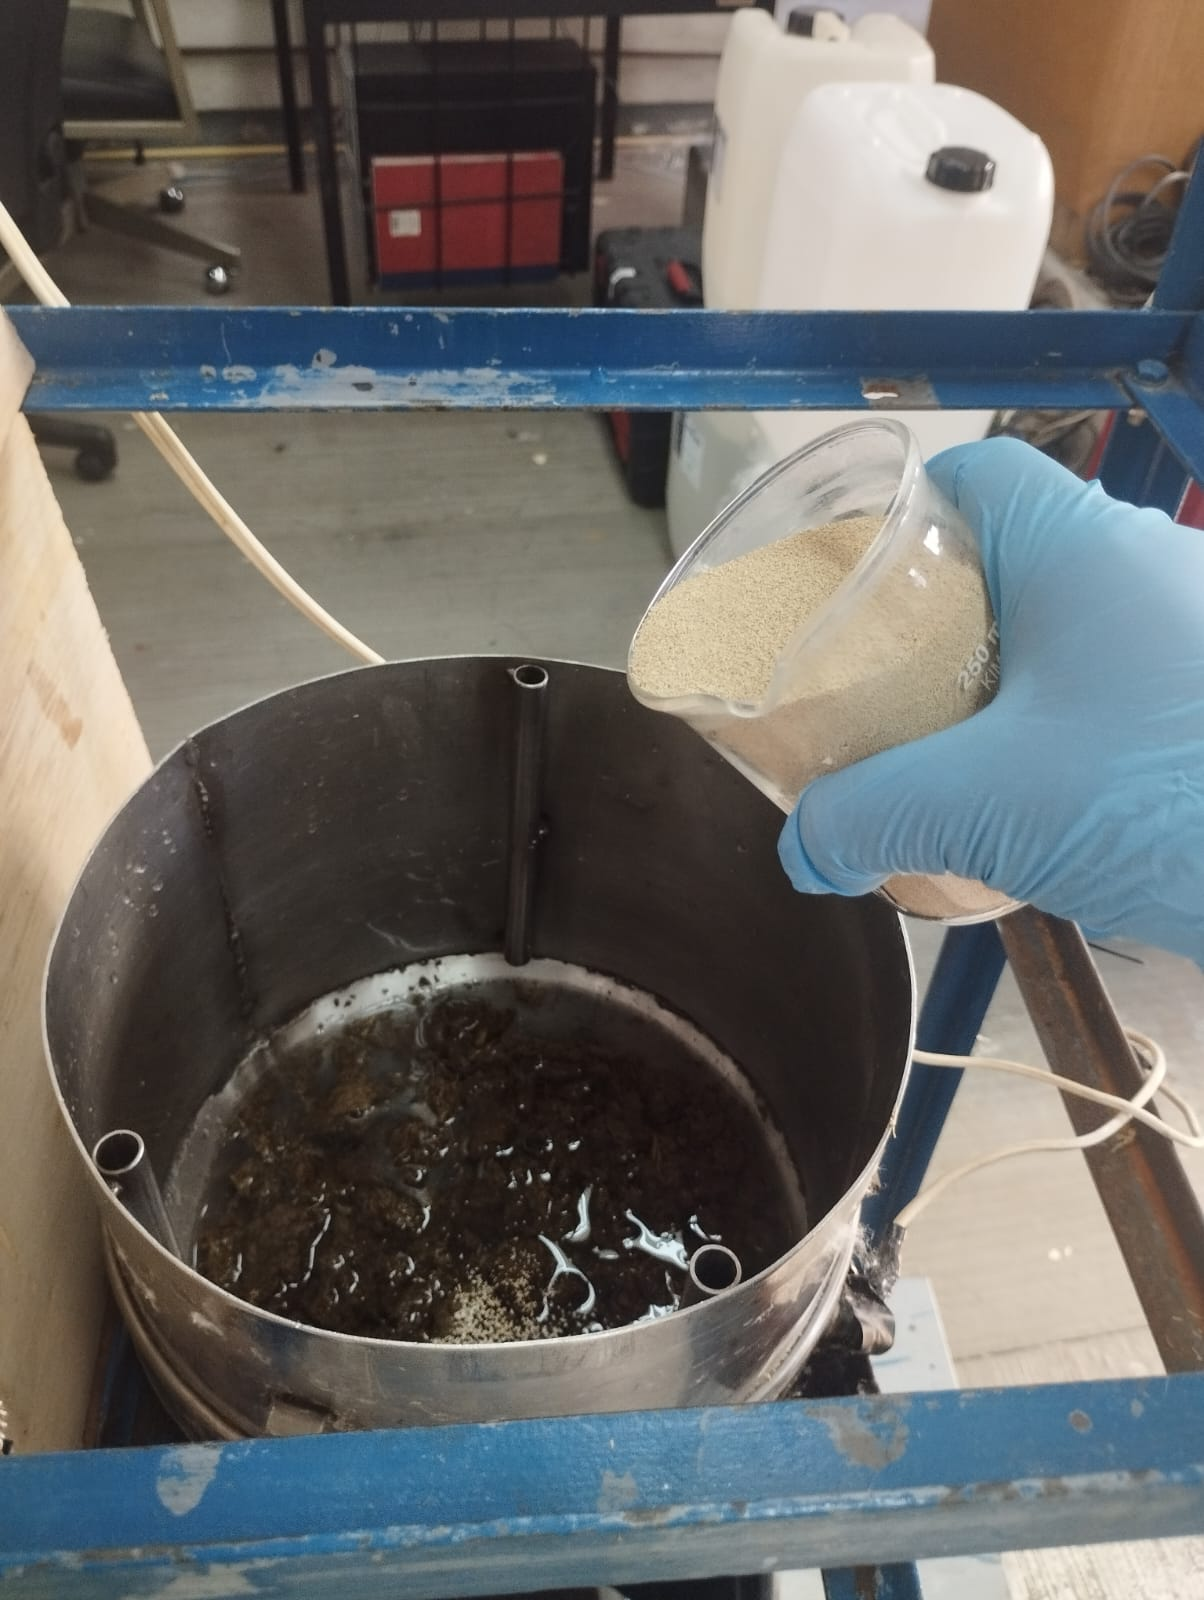
\includegraphics[width=4cm, height=3cm]{imagenes/hidrolisis4 } % Cambia "imagen2.jpg" por el nombre de tu archivo
	     		\caption{La levadura se agrega al reactor.}
	     		\label{hidrolisis4}
	     	\end{minipage}
	     \end{figure}
	     
	     
	     \textbf{5.} Con ayuda de una micropipeta calibrada se midieron los mililitros exactos de la enzima Cellic CTec2 según el diseño de experimentos, la cual se añadió al sistema y se mezcló meticulosamente hasta su completa integración (Figura \ref{hidrolisis9}), asegurando la actividad enzimática óptima	\\ 
	     	
	     	 
	     \textbf{6.} El pH de la mezcla se midió utilizando un medidor de pH Hanna Instruments previamente calibrado, introduciendo el electrodo en la solución y agitando suavemente para obtener una lectura estable; dependiendo del resultado, se añadió gradualmente ácido cítrico en cantidades pesadas con precisión, monitoreando el cambio en el pH después de cada adición hasta alcanzar el valor deseado según los parámetros establecidos en el diseño experimental, ver figura \ref{hidrolisis3}.
	     
	     
	     
	     \begin{figure}[H]
	     	\centering
	     	\begin{minipage}{0.46\textwidth}
	     		\centering
	     		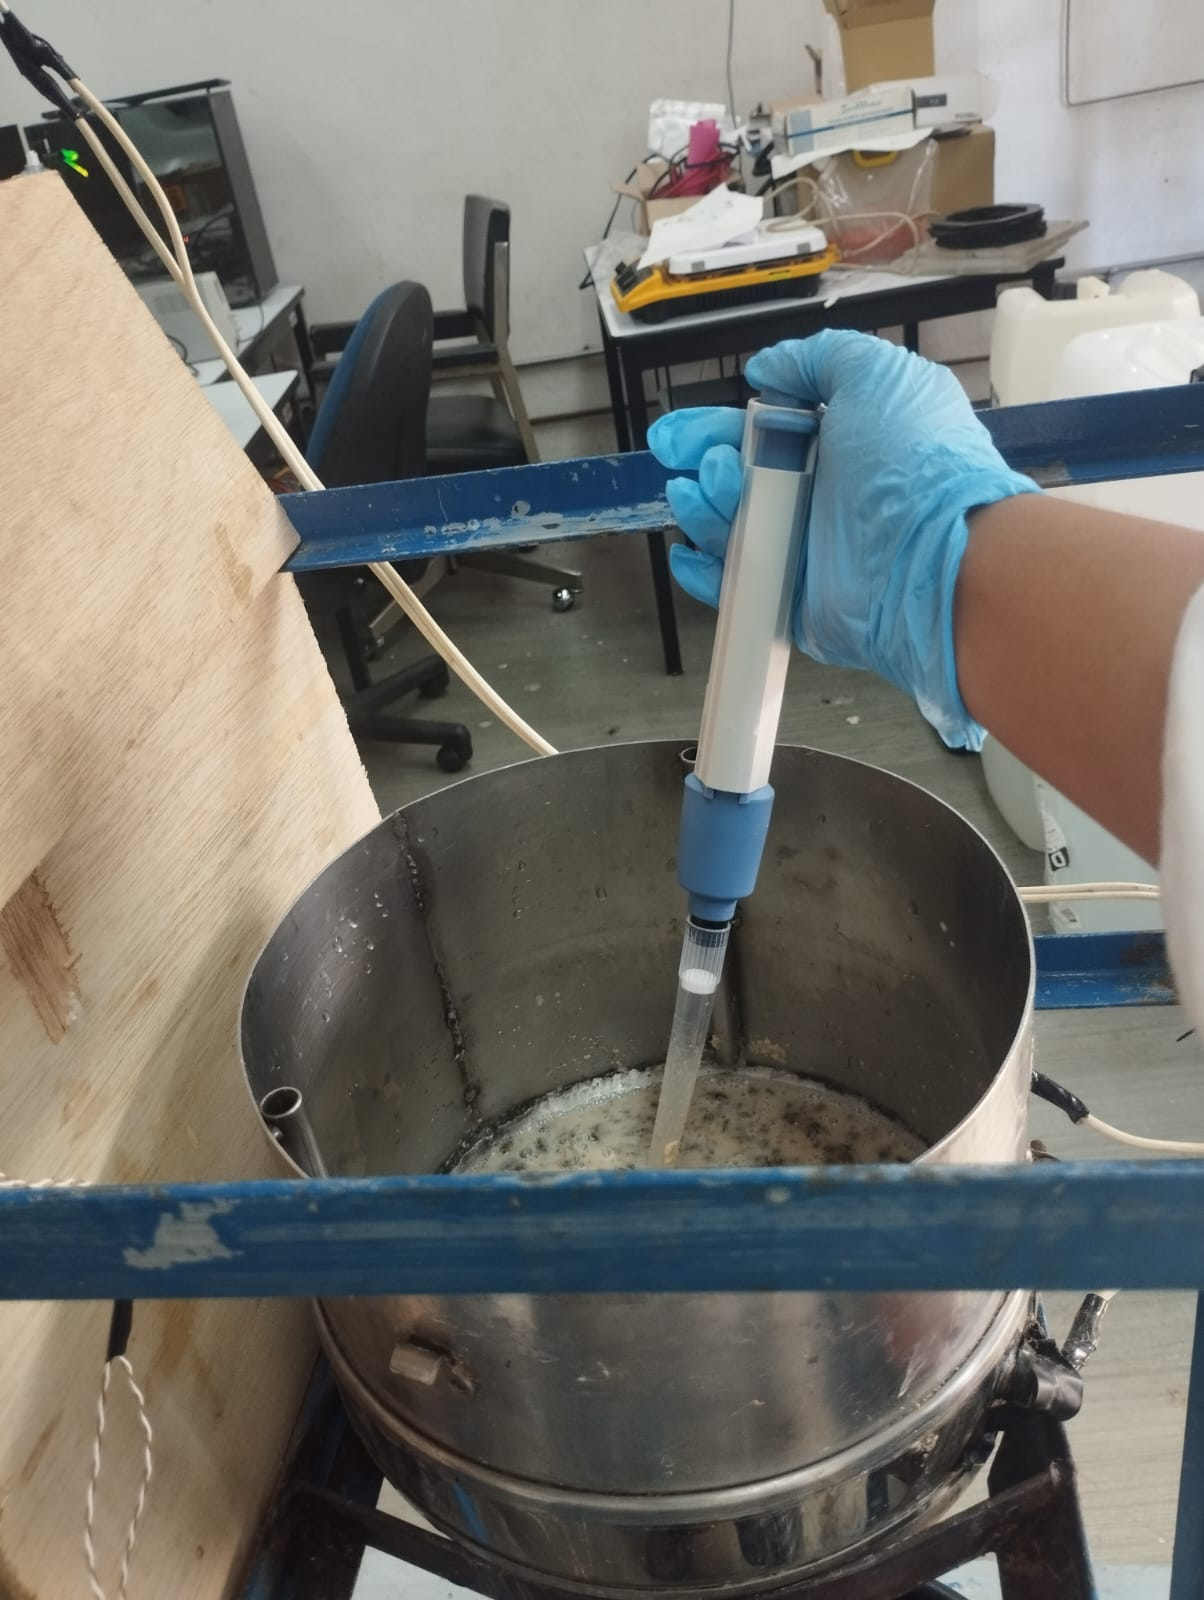
\includegraphics[width=5cm, height=3cm]{imagenes/hidrolisis9} % Cambia "imagen1.jpg" por el nombre de tu archivo
	     		\caption{ Se agrega la enzima al reactor con ayuda de la micropipeta. }
	     		\label{hidrolisis9}
	     	\end{minipage}
	     	\hfill
	     	\begin{minipage}{0.48\textwidth}
	     		\centering
	     		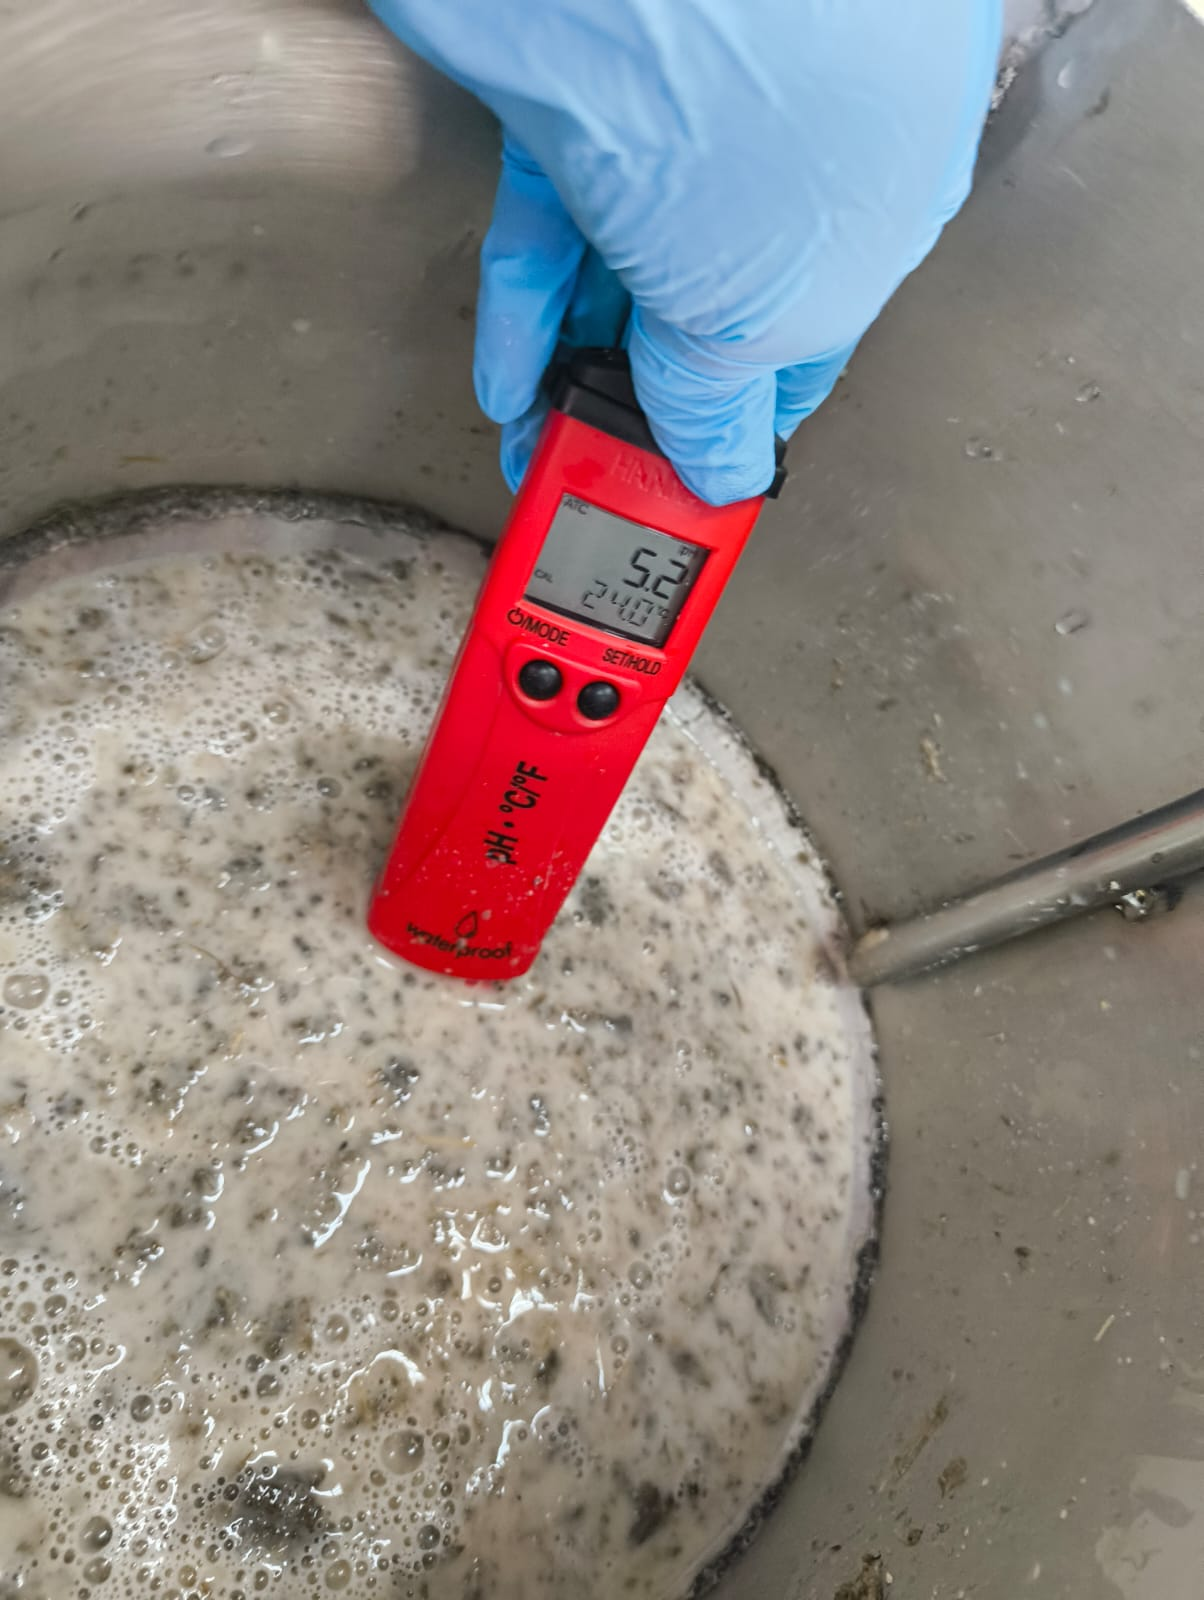
\includegraphics[width=5cm, height=3cm]{imagenes/hidrolisis3 } % Cambia "imagen2.jpg" por el nombre de tu archivo
	     		\caption{ Se mide el ph de la mezcla con ayuda del medidor hanna instruments.}
	     		\label{hidrolisis3}
	     	\end{minipage}
	     \end{figure}
	     
	      \textbf{7.} El reactor tipo batch se selló herméticamente utilizando algodón y papel aluminio (ver Figura \ref{hidrolisis 6}), y se instaló una trampa de aire compuesta por una manguera insertada en uno de los orificios de la tapa del reactor. Para garantizar un cierre seguro y evitar fugas, se reforzó la conexión entre la manguera y la tapa con cinta adhesiva. El extremo libre de la manguera se sumergió en una cubeta con agua, permitiendo la liberación controlada del dióxido de carbono generado durante la reacción, al mismo tiempo que impidió la entrada de oxígeno al sistema. Este diseño asegura un ambiente anaeróbico adecuado para el proceso.
	      \\[0.5em]
	     
	     	\textbf{8.} Se inició el sistema de control para la SSF, ajustando los parámetros de tiempo y temperatura según las condiciones predefinidas en el diseño experimental (ver apartado \ref{SacariSF}), garantizando así las condiciones adecuadas para el proceso. Ver Figura \ref{hidrolisis 8} para observar la estructura y conexiones.
	     	
	 
	     		     \begin{figure}[H]
	     		\centering
	     		\begin{minipage}{0.46\textwidth}
	     			\centering
	     			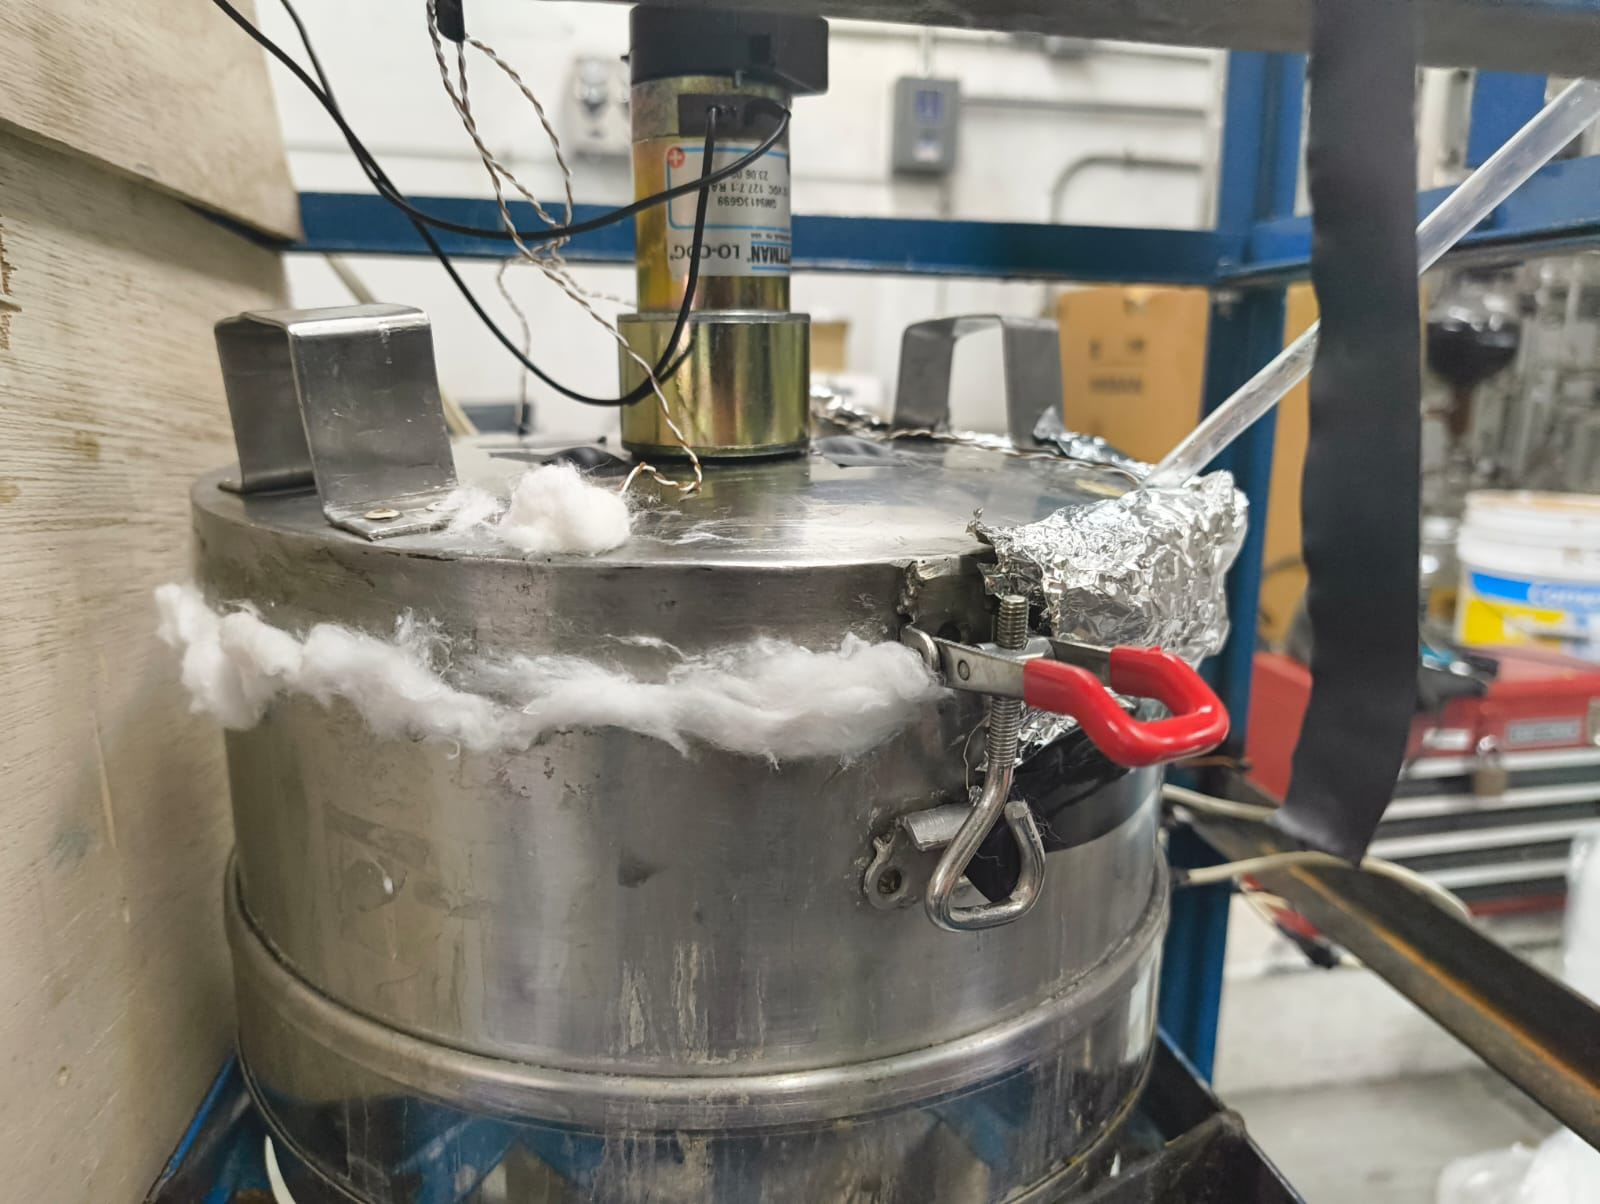
\includegraphics[width=5cm, height=3cm]{imagenes/hidrolisis 6} % Cambia "imagen1.jpg" por el nombre de tu archivo
	     			\caption{ El algodón es colocado entre la tapa para tratar de que el reactor sea lo mas hermético posible. }
	     			\label{hidrolisis  6}
	     		\end{minipage}
	     		\hfill
	     		\begin{minipage}{0.48\textwidth}
	     			\centering
	     			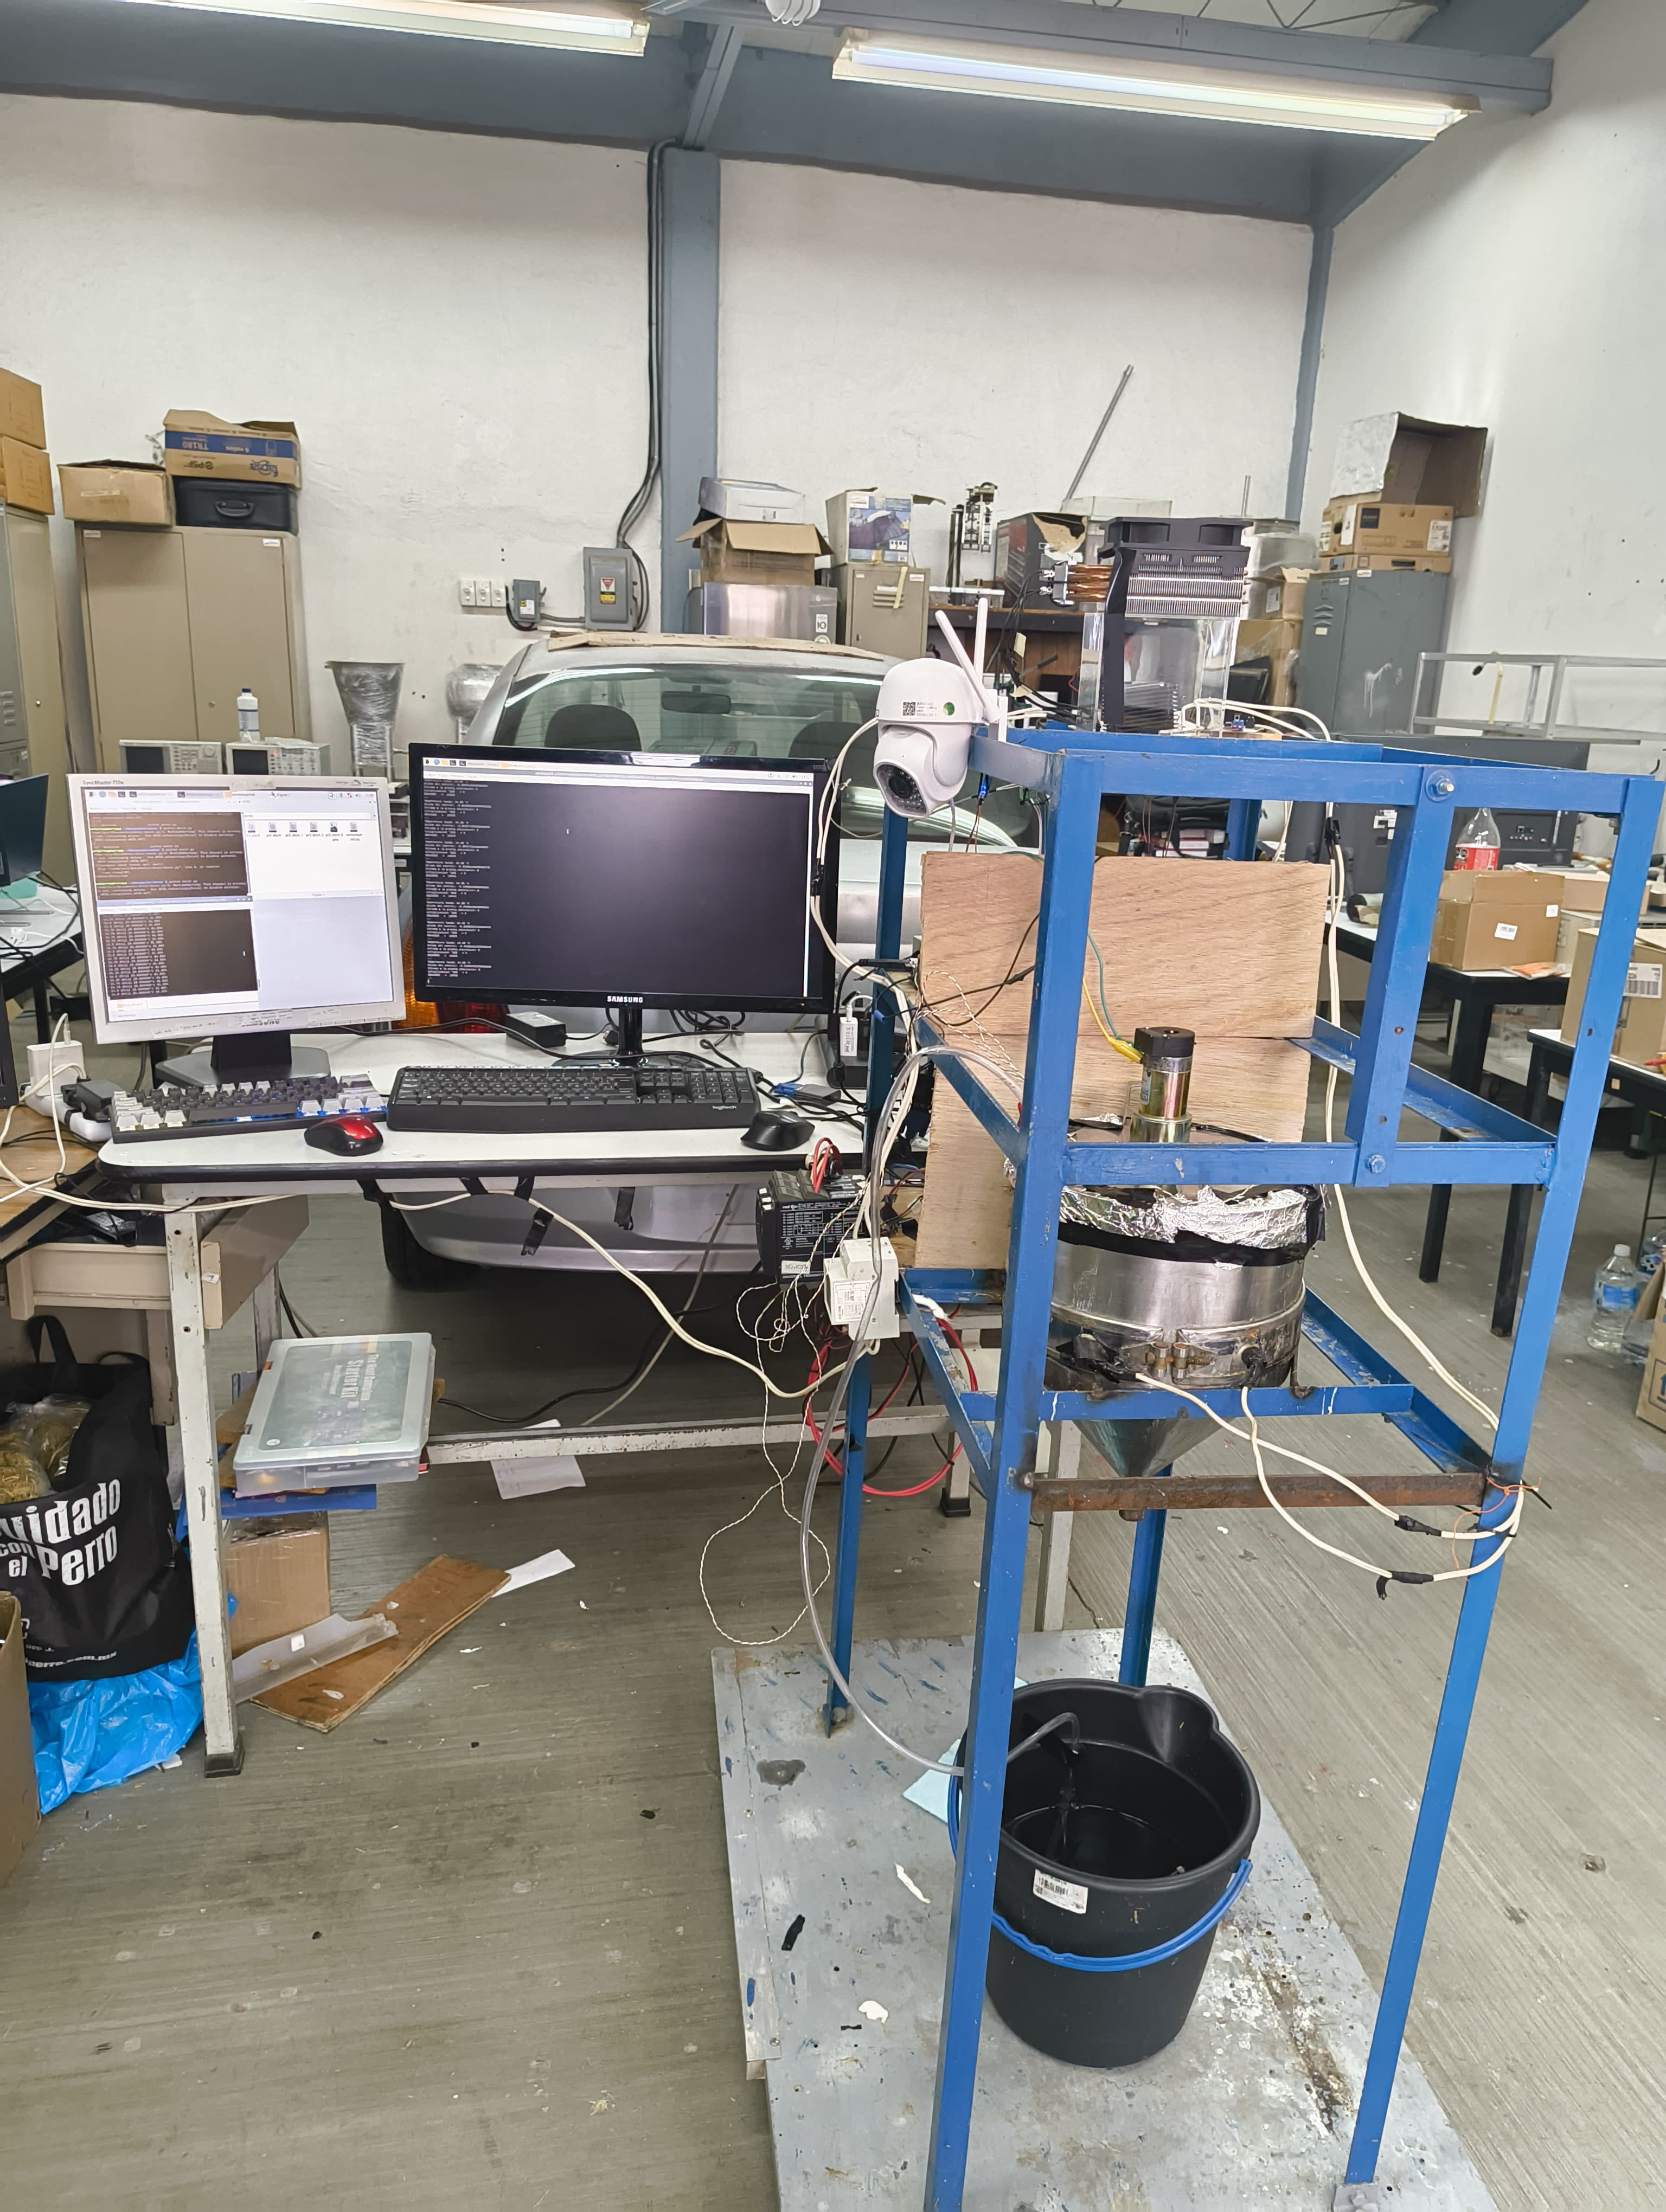
\includegraphics[width=3cm, height=3cm]{imagenes/conexion de hidrolisis } % Cambia "imagen2.jpg" por el nombre de tu archivo
	     			\caption{ Puesta en marcha del control en la etapa de SSF en un reactor tipo batch.}
	     			\label{hidrolisis 8}
	     		\end{minipage}
	     	\end{figure}
	     	
	     	
	     	\textbf{9.} Finalizado el proceso de SSF, se determina el pH final del producto (Figura \ref{hidrolisis 7}) y se transfiere a recipientes herméticos, los cuales se almacenan a temperaturas inferiores a 30 °C para preservar las muestras hasta la cuantificación del contenido alcohólico con ayuda de un refractometro manual. Finalmente el reactor tipo batch es lavado con agua desmineralizada.
	     	
	     	
	     		   	\begin{figure}[H]
	     		\centering
	     		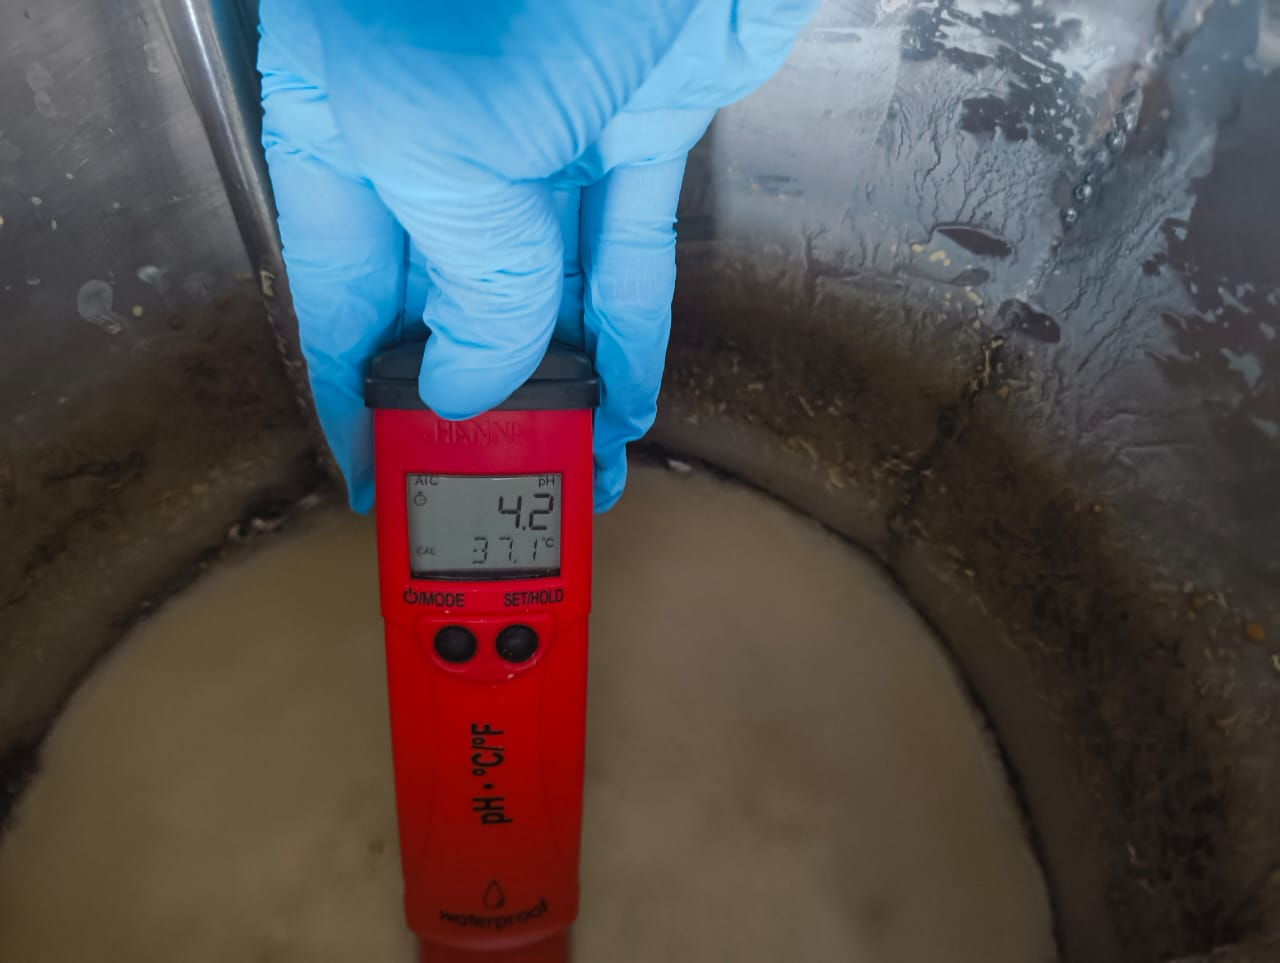
\includegraphics[width=5cm, height=3cm]{imagenes/hidrolisis7}
	     		\caption{ Medición del ph de la mezcla después de la SSF.}
	     		\label{hidrolisis 7}
	     	\end{figure}
	     	
	     	
	     	\textbf{10.} El diseño del control del proceso SSF se reporta en el anexo \ref{diseño del control de temp}.
	     	
	     	
			%%%%%%%%%%%%%%%%%%%%%%%%%%%%%%%%%%%%%%%%%%%%%%%%%%%%%%%%%%%%%%%%%%%%%
			
			
			%%%%%%%%%%%%%%%%%%%%%%%%%%%%%%%%%%%%%%%%%%%%%%%%%%%%%%%%%%%%%%%%%%%%%%%%%%%%%%%%%%%%%%%%%%%%%%%%%%%%%%%%%%%%%%%%%%%%%%%%%%%%%%%%%%%%%%%%%%%%%%%%%%%%%%%%%%%%%%%%%%%%%%%%%%%%%%%%%%%%%%%%%%%%%%%%%%%%%%%%%%%%%%%%%%%%%%%%%%%%%%%%%%%%%%%%%%%%%%%%%%%%%%%%%%%%%%%%%%%%%%%%%%%%%%%%%%%%%%%%%%%%%%%%%%%%%%%%%%%%%%%%%%%%%%%%%%%%%%%%%%%%%%%%%%%%%%%%%%%%%%%%%%%%%%%%%%%%%%%%%%%%%%%%%%%%%%%%%%%%%%%%%%%%%%%%%%%%%%%%%%%%%%%%%%%%%%%%%%%%%%%%%%%%%%%%%%%%%%%%%%%%%%%%%%%%%%%%%%%%%%%%%%%%%%%%%%%%%%%%
		

				\subsection{Resultados experimentales del proceso de producción de bioetanol 2 G con pretratamiento Alcalino  y Biológico}
				En esta Sección se reportan los resultados de los experimentos implementados en un reactor tipo batch de laboratorio con capacidad de 6 L para producir bioetanol de segunda generación a partir de bagazo de caña. Se compara el desempeño de dos alternativas de producción: un pretratamiento biológico seguido de un proceso SSF, y un pretratamiento alcalino seguido de un proceso SSF. La misma configuración de producción conduce a diferentes desempeños del proceso, distinguiendo los pretratamientos. Los resultados se presentan en téminos de la calidad del producto, el consumo energético y los costos de producción. Los desempeños presentados corresponden al producto y condiciones de operación de los experimentos diseñados en el apartado \ref{Diseño factorial del pretratamiento alcalino}.
				
				
				
		
		\subsubsection{Pretratamiento Biológico}
	Los pretratamientos biológicos realizados sobre bagazo de caña de azúcar (Tabla \ref{Pretratamiento Biológico}) comprendieron tres pruebas con granulometría de TNUB (1 mm - 10 cm) y tres pruebas con granulometría de 1 cm, bajo temperaturas controladas (30, 40 y 45 °C), registrándose el consumo energético (kWh) en cada caso. Este diseño experimental permitió evaluar comparativamente las diferencias en los costos asociados al consumo energético derivado principalmente el calentamiento del bioreactor a la temperatura de diseño para el procesamiento de la biomasa, específicamente se considera el consumo de la resistencia de calentamiento y del convertidor para implementar el control de temperatura durante toda la etapa de pretratamiento. 
		
	\begin{table}[H]
		\centering
		\caption{Preubas experimentales con pretratamiento biológico.}
		\begin{tabular}{|c|c|c|c|}
			\hline
			\textbf{Num de} &\textbf{ Temperatura} & \textbf{Tamaño de bagazo} & \textbf{Consumo energético } \\ 
			\textbf{de experimento} &\textbf{  (°C)} &  & \textbf{ (kWh)} \\ \hline
			1 & \multirow{2}{*}{45} & TNUB & 4.55 \\ \cline{1-1} \cline{3-4}
			2 &  & 1 cm & 3.81 \\ \hline
			3 &\multirow{2}{*}{ 40} & TNUB & 2.77 \\ \cline{3-4} \cline{1-1}
			4 &  & 1 cm & 2.81 \\ \hline
			5 &\multirow{2}{*}{ 30} & TNUB & 4.55 \\ \cline{3-4}\cline{1-1}
			6 &  & 1 cm & 1.11 \\ \hline
		\end{tabular}
		\label{Pretratamiento Biológico}
	\end{table}
	
	El tiempo de pretratamiento para las pruebas anteriores fue 5 días
		%%%%%%%%%%%%%%%%%%%%%%%%%%%%%%%%%%%%%%%%%%%%%%%%%%%%%%%%%%%%%%%%%%%%%%%%%%%
		
		\subsubsection{Pretratamiento Alcalino}
		
		
		Inicialmente se definió un tiempo para el pretratamiento alcalino según lo recomendado por \cite{Arturo2022evaluacion}, quien consideró condiciones reportadas en la literatura. En la práctica, ya que el proceso se llevó a cabo en la presente tesis usando un reactor más grande que el empleado en el trabajo de referencia, el control de temperatura se volvió crítico. El control de temperatura que fue implementado tiene un tiempo de establecimiento relativamente grande, durante el cual la temperatura no se encuentra todavía en la referencia. Un supuesto fue que un tiempo de pretratamiento más largo permitiría operar por más tiempo el reactor con la temperatura controlada, y que esta etapa podría resultar más efectiva. En concreto, como segunda condición se definió un tiempo de pretratamiento de 7870, manejando partículas de bagazo de caña de 1 mm hasta 10 cm. Los tamaños considerados fueron iguales al caso previo con pretratamiento biológico, se manejaron tamaños no uniformes de bagazo (TNUB) y partículas de 1 cm. En la Tabla \ref{Pretratamiento Alcalino} se muestran las condiciones de los 12 experimentos diseñados, indicando la energía consumida en cada una de las pruebas, expresada en unidades de kWh, la cual fue leída de un watimetro. Esta energía también corresponde al consumo debido al calentamiento del reactor, sumando específicamente el consumo de la resistencia de calentamiento y del convertidor del control durante el pretratamiento.
		
		
		\begin{table}[H]
			\centering
			\caption{Preubas experimentales con pretratamiento alcalino}
			\begin{tabular}{|c|c|c|c|c|}
				\hline
				\textbf{Num de} & \textbf{Temperatura} & \textbf{Tamaño de } & \textbf{Tiempo} & \textbf{Consumo } \\ 
			\textbf{de experimento}	&\textbf{ (°C)}&\textbf{ bagazo}  &\textbf{(s)}	&\textbf{ energético (kWh)}\\ \hline
				1 & \multirow{4}{*}{95} & \multirow{2}{*}{TNUB} & 5400 & 0.66  \\ \cline{1-1} \cline{4-5}
				2 &  &  & 7870 & 0.81  \\ \cline{3-5}  \cline{1-1} 
				3 &  & \multirow{2}{*}{1 cm} & 5400 & 0.74 \\  \cline{1-1} \cline{4-5}
				4 &  &  & 7870 & 0.86 \\ \cline{1-1}  \hline
				5 & \multirow{4}{*}{90}& \multirow{2}{*}{TNUB} & 5400 & 0.71  \\ \cline{1-1}  \cline{4-5}
				6 &  &  & 7870 & 0.7  \\ \cline{1-1} \cline{3-5}
				7 &  & \multirow{2}{*}{1 cm} & 5400 & 0.74 \\ \cline{1-1}\cline{4-5}
				8 &  &  & 7870 & 0.6 \\ \hline
				9 & \multirow{4}{*}{80} & \multirow{2}{*}{TNUB} & 5400 & 0.67  \\ \cline{1-1}\cline{4-5}
				10 &  &  & 7870 & 0.63  \\ \cline{1-1} \cline{3-5}
				11 &  &\multirow{2}{*}{1 cm} & 5400 & 0.78 \\ \cline{1-1}\cline{4-5}
				12 &  &  & 7870 & 0.8 \\ \hline
			\end{tabular}
			\label{Pretratamiento Alcalino}
		\end{table}
		
		
		
		
	
	%%%%%%%%%%%%%%%%%%%%%%%%%%%%%%%%%%%%%%%%%%%%%%%%%%%%%%%%%%%%%%%%%%%%%%%%%%%%%%%%%%%%%%%%%%%%%%%%%%%%%%%%%%%%%%%%%%%%
	\subsection{Resultados experimentales del proceso de producción de bioetanol en la etapa de hidrólisis y fermentación utilizando diferentes tipos de pretratamiento}
A continuación se presentan los resultados de las pruebas experimentales de la etapa SSF. Los datos reportados son la cantidad de alcohol obtenida, así como el consumo energético para las dos etapas del proceso .
			%%%%%%%%%%%%%%%%%%%%%%%%%%%%%%%%%%%%%%%%%%%%%%%%%%%%%%%%%%%%%%%%%%%%%%%%%%%%%%%%%%%%%%%%%%%%%%%%%%%%%%%%%%%%%%%%%%%%%%%%%%%%%%%%%%%%%%%%%%%%%%%%%%%%%%%%%%%%%%%%%%%%
   	\subsubsection{ Hidrólisis y fermentación para pretratamiento Biológico}
   
Cada pretratamiento realizado fue seguido de una hidrólisis y fermentación simultáneas. En la Tabla \ref{ssf Pretratamiento Biológico} se presentan las condiciones de las 6 pruebas con pretratamiento biológico de la biomasa. De las pruebas se registró la energía consumida por etapa, dada en kWh, y el contenido de ethanol en el producto.

 	\begin{table}[H]
 		\centering
 		\caption{SSF con pretratamiento biológico.}
 		\begin{tabular}{|c|c|c|c|c|c|}
 			\hline
 			\textbf{Num }& \textbf{Temperatura}  & \textbf{Tamaño} & \textbf{Consumo } & \textbf{Consumo }  & \textbf{Producción} \\ 
 			\textbf{de}&\textbf{(°C)} &\textbf{de bagazo} & \textbf{energético} & \textbf{energético }&\textbf{de alcohol}\\ 
 				\textbf{exp.}&& & \textbf{ pretrata (kWh)} & \textbf{ SSF (kWh)}&\textbf{(\%)}\\ \hline
 			
 			1 & \multirow{2}{*}{45} & TNUB & 4.55 & 2.8  & 11.5 \\ \cline{1-1} \cline{3-6}
 			2 &                     & 1 cm & 3.81 & 2.7  & 14 \\ \hline
 			3 & \multirow{2}{*}{40} & TNUB & 2.77 & 2.56 & 11 \\ \cline{1-1} \cline{3-6}
 			4 &                     & 1 cm & 2.81 & 1.74  & 11 \\  \hline
 			5 & \multirow{2}{*}{30} & TNUB & 4.55 &2.7  & 11 \\ \cline{1-1} \cline{3-6}
 			6 &                     & 1 cm & 1.11 &3.01 & 11 \\ \hline
 		\end{tabular}
 		\label{ssf Pretratamiento Biológico}
 	\end{table}
 	
 
 	
 	
 

 	%%%%%%%%%%%%%%%%%%%%%%%%%%%%%%%%%%%%%%%%%%%%%%%%%%%%%%%%%%%%%%%%%%%%%%%%%%%%%%%%%%%%%%%%%%%%%%%%%%%%%%%%%%%%%%%%%%%%%%%%%%%%%%%%%%%%%%%%%%%%%%%%%%%%%%%%%%%%%%%%%%%%%%%
 	
		\subsubsection{ Hidrólisis y fermentación para pretratamiento Alcalino}
		
		Para las pruebas de SSF con bagazo pretratado con hidróxido de sodio, se utilizó lo reportado en el diseño de experimentos en el apartado \ref{SacariSF}, la Tabla \ref{ssf con Pretratamiento Alcalino}  muestra las pruebas con bagazo de 1 mm hasta 10 cm y 1 cm como tamaño de partícula. De las pruebas podemos observar que el cambio de temperatura del pretratamiento si influye en el resultado de la producción de bioetanol.
		
		
		\begin{table}[H]
			\centering
			\caption{SSF con pretratamiento alcalino.}
			\begin{tabular}{|c|c|c|c|c|c|c|}
				\hline
				\textbf{Num} & \textbf{Temperatura} & \textbf{Tamaño} & \textbf{Tiempo} & \textbf{Consumo } & \textbf{Consumo } & \textbf{Producción } \\
			\textbf{de}	&\textbf{ (°C)}& \textbf{bagazo}&\textbf{(s)}	&\textbf{de pretra. }&\textbf{ de SSF}&\textbf{ de alcohol}\\ 
				\textbf{exp}	& & \textbf{bagazo}&	&\textbf{ (kWh)}&\textbf{ (kWh)}&\textbf{ (\%)}\\ \hline
			
			
				1 & \multirow{4}{*}{95} & \multirow{2}{*}{TNUB} & 5400 &0.66& 1.95 & 13 \\ \cline{1-1} \cline{4-6}
				2 &                     &                       & 7870 &0.81& 2.74 & 13 \\ \cline{3-6}  \cline{1-1}
				3 &                     &\multirow{2}{*}{1 cm}  & 5400 &0.74& 1.41 & 10 \\ \cline{4-6}  \cline{1-1}
				4 &                     &                       & 7870 &0.86& 2.78 & 17 \\ \hline
				5 & \multirow{4}{*}{90} & \multirow{2}{*}{TNUB} & 5400 &0.71& 1.87 & 12 \\  \cline{1-1} \cline{4-6}
				6 &                     &                       & 7870 &0.7& 1.88 & 13 \\ \cline{1-1} \cline{3-6}
				7 &                     & \multirow{2}{*}{1 cm} & 5400 &0.74& 2.63 & 13 \\ \cline{1-1} \cline{4-6}
				8 &                     &                       & 7870 & 0.6&2.88 & 11 \\ \hline
				9 &\multirow{2}{*}{80 } & TNUB                  & 5400 &0.67 &1.84 & 13 \\ \cline{1-1} \cline{3-6}
				10 &                     & 1 cm                 & 7870 & 0.8&2.58 & 13 \\ \hline
			\end{tabular}
			\label{ssf con Pretratamiento Alcalino}
		\end{table}
		
		
 Como podemos observar en la Tabla \ref{ssf con Pretratamiento Alcalino} se realizaron 10 pruebas de las 12 planeadas debido a un problema con los insumos y el biorreactor, sin embargo podemos concluir que un tiempo de 7870 mejora la producción de bioetanol.
				
		
		
		
		
			%%%%%%%%%%%%%%%%%%%%%%%%%%%%%%%%%%%%%%%%%%%%%%%%%%%%%%%%%%%%%%%%%%%%%%%%%%%%%%%%%%%%%%%%%%%%%%%%%%%%%%%%%%%%%%%%%%%%%%%%%%%%%%%%%%%%%%%%%%%%%%%%%%%%%%%%%%%%%%%%%%%%%%%%%%%%
			
			\subsection{Costos en la producción de bioetanol}
	Para conocer cuánto nos cuesta realizar las pruebas de producción de bioetanol aplicando pretratamientos biológicos y alcalinos, se realizaron un análisis de costos y una comparación de los mismos.
	El ccosto del consumo energético (kWh) se calculó a partir de la tarifa industrial de \$1.348 MXN/kWh o \$ 0.06 USD/kWh, establecida por la Comisión Federal de Electricidad, por sus siglas, CFE  \cite{CFE2023}, en media tensión en Cuernavaca, Morelos. Se consideró como referencia el mes de abril de 2025. Este precio se aplicó a todas las etapas del proceso, desde los pretratamientos hasta la hidrólisis y fermentación. Los costos están expresados en dólares estadounidenses (USD), con una tasa de cambio de 1 USD = 20.84 MXN, vigente al 8 de abril de 2025.
			
		
	 \subsubsection{Costos en la producción de bioetanol solo para pretratamiento biológico}
			
			
Para la producción de bioetanol utilizando un pretratamiento biológico, fue necesario considerar los costos asociados, que abarcan tanto la adquisición de materiales como el consumo energético requerido. Los resultados demuestran que la inversión total requerida para los materiales necesarios en el proceso de pretratamiento biológico, asciende a \$5.74 USD. Los detalles se dan en  la Tabla 	\ref{tab:costos_completos}.

\begin{table}[H]
	\centering
	
	\caption{Costos detallados de materiales.}
	\label{tab:costos_completos}
	\footnotesize
	\setlength{\tabcolsep}{2.5pt}
	\begin{tabular}{|l|c|c|c|c|}
		\hline
		\multirow{2}{*}{\textbf{Material}} & \textbf{Costo} & \textbf{Cantidad} &  \textbf{Costo de lo} \\
		& \textbf{ de kg/L} & \textbf{ por pretratamiento}  &  \textbf{utilizado más} \\
		& \textbf{ (\$ USD)} & \textbf{(g/ml)}  & \textbf{envío (\$ USD)} \\
		\hline
		\textbf{Humus de lombriz} & 0.29 & 300 g &   0.16 \\
		\hline
		\textbf{Bagazo de caña} & 0.95 & 180 g &   0.19 \\
		\hline
		\textbf{Agua desmineralizada} & 0.68 & 6000 ml &  5.38 \\
		\hline
	\end{tabular}
\end{table}

Al realizarse las pruebas experimentales en el reactor tipo batch se registró el consumo energético, a continuación en la Tabla \ref{tabla de energia} se presenta el costo que representa ese consumo energético.
	
	
	\begin{table}[H]
		\centering
		\caption{Energía consumida para pretratamiento biológico  y su costo en (\$ USD). }
		\label{tabla de energia}
	\setlength{\tabcolsep}{2.5pt}
		\begin{tabular}{|c|c|c|c|c|}
			\hline
		\textbf{Num de}&\textbf{Temperatura del} & \textbf{Tamaño }  & \textbf{ Consumo } & \textbf{Costos } \\ 
			&\textbf{ pretratamiento (°C)} &	\textbf{ de bagazo}  & 	\textbf{energético(kWh) }& 	\textbf{(\$ USD)} \\ \hline
     1  & \multirow{2}{*}{95} & TNUB & 4.55 & 0.294 \\ \cline{3-5} \cline{1-1}
2	& & 1cm & 3.81 & 0.246 \\ \hline 
3&\multirow{2}{*}{90} & TNUB & 2.77 & 0.179 \\ \cline{3-5} \cline{1-1}
4	& & 1cm & 2.81 & 0.181  \\ \hline 
5&\multirow{2}{*}{80}	 & TNUB & 0.75 & 0.048  \\ \cline{3-5} \cline{1-1}
6&	 & 1cm & 1.11 & 0.071  \\ 	\hline		
		\end{tabular}
	
	\end{table}
	
	
De los resultados obtenidos se desprende que el consumo energético promedio requerido para el pretratamiento biológico asciende a 2.43 kWh, lo que representa un costo promedio de \$0.157 USD (Cero punto ciento cincuenta y siete dólares) por prueba experimental.

	%%%%%%%%%%%%%%%%%%%%%%%%%%%%%%%%%%%%%%%%%%%%%%%%%%%%%%%%%%%%%%%%%%%%%%%%%%%%%%%%%%%%%%%%%%%%%%%%%%%%%%%%%%%%%%%%%%%%%%%%%%%%%%%%%%%%%%%%%%%%%%%%%%%%%%%%%%%%%%%%%%%%%%%%%%%%%%%%%%%%%%%%%%%%%%%%%%%%%%
	
		\subsubsection{Costos en la producción de bioetanol con pretratamiento Alcalino }
	
	Para la producción de bioethanol aplicando el pretratamiento alcalino se utilizaron los insumos que se muestran en a continuación en la Tabla \ref{Costo para pretratamiento alcalino}, cuyos costos unitarios (por kilogramo o litro, según el caso) se especifican en la misma Tabla.
	
	
	
	\begin{table}[H]
		\centering
		\caption{Costos para la producción de bioetanol con pretratamiento alcalino.}
		\label{Costo para pretratamiento alcalino}
		\setlength{\tabcolsep}{2.5pt}
		\begin{tabular}{|c|c|c|c|}
			\hline
			& \textbf{Costo}& \textbf{Cantidad utilizada }  & \textbf{ Costo} \\
			\textbf{Material}&	\textbf{kg/L} & 	\textbf{por pretratamiento}& \textbf{pretratamiento} \\ 
			\textbf{(\$ USD) }		& \textbf{(\$ USD)} &\textbf{	(\$ USD) }& \textbf{	(\$ USD) }\\ \hline		
			Hidróxido de sodio&37.9& 120 g&5.067178503 \\ \hline
			Bagazo de caña 	  &0.95& 240 g &  0.253358925 \\ \hline
			Agua desmineralizada&0.68& 6000 ml  & 5.38 \\ \hline
		\end{tabular} 
		
		
	\end{table}
	De acuerdo con los datos obtenidos, se determinó el costo asociado a los materiales utilizados en cada prueba experimental. Los resultados se presentan en la columna 4 de la Tabla \ref{Costo para pretratamiento alcalino}. Adicionalmente, se consideró el costo de envío de cada insumo, el cual fue puesto en función de la cantidad empleada específicamente en el pretratamiento. Este valor se adicionó al costo del material utilizado por prueba. El resltado se refiere a los costos de producción, tomando en cuenta los insumos, descritos.

	El análisis económico revela que, al sumar los costos de consumo y envío de todos los materiales, se obtiene un costo total por prueba de \$10.7 USD. Es importante señalar que este cálculo no incluye los gastos asociados al consumo energético requerido para la producción de bioetanol de segunda generación. Este desglose financiero permite una evaluación precisa de los recursos invertidos en la etapa de pretratamiento alcalino.
	
	La Tabla \ref{tabla costo 1 cm} documenta el consumo energético promedio de 0.744 kWh (equivalente a \$0.048 USD por prueba) en pretratamientos alcalinos con bagazo de 1 cm.
	
	
	
	\begin{table}[H]
		\centering
		\caption{Energía consumida para pretratamiento alcalino para bagazo de caña y su costo en \$ USD. }
		\label{tabla costo 1 cm}
		\setlength{\tabcolsep}{2.5pt}
			\begin{tabular}{|c|c|c|c|c|c|}
				\hline
				\textbf{Num}&\textbf{Temperatura } & \textbf{Tamaño } & \textbf{Tiempo} & \textbf{Energía} & \textbf{Costos } \\ 
			\textbf{ de}	&\textbf{pretratamiento } &	\textbf{ de}  &	\textbf{ (s)} & 	\textbf{ consumida }& 	\textbf{(\$ USD)} \\ 
			\textbf{exp}	&\textbf{(°C)} &	\textbf{ bagazo}  &	 & 	\textbf{ Pretrata(kWh) }& 	 \\ \hline
			
			
			1&	\multirow{5}{*}{95} & \multirow{3}{*}{TNUB} & 5400 &0.66  & 0.88968  \\  \cline{4-6} \cline{1-1}
			2&                     	&                       & 7870 &0.81 & 1.09188  \\ \cline{3-6} \cline{1-1}
			3&                     	& \multirow{3}{*}{1 cm} & 5400 &0.74 & 0.04786  \\  \cline{4-6} \cline{1-1}
			4&                   	&                       & 7870 & 0.86 & 0.055  \\  \hline 
			5&\multirow{5}{*}{90}   & \multirow{3}{*}{TNUB} & 5400 & 0.66  &0.88968  \\  \cline{4-6} \cline{1-1}
			6&                  	&                       & 7870 & 0.7  &  0.9436  \\ 	\cline{3-6} \cline{1-1}
			7&                  	& \multirow{2}{*}{1 cm} & 5400 & 0.6& 0.0388   \\  \cline{4-6} \cline{1-1}
			8&	                    &                       & 7870 & 0.74 & 0.047865\\   \hline
			9&	\multirow{2}{*}{80} & TNUB                  & 5400 &  0.67 & 0.90316  \\  \cline{3-6} \cline{1-1}
			10&	                    & 1 cm                  & 7870 & 0.78 & 0.05045 \\ \hline
		\end{tabular}
		
	\end{table}
	
	
	La Tabla \ref{tabla costo 1 cm} integra el consumo energético (kWh) y su costo equivalente en pesos mexicanos para el pretratamiento de bagazo de caña con granulometrías entre 1 mm y 10 cm. El consumo promedio para pretratamiento utilizando bagazo de 1 mm hasta 10 cm de bagazo, según las pruebas realizadas que se muestran es de 0.67 kWh, y el costo promedio por prueba es de \$0.045 MXN.
	
	
	%%%%%%%%%%%%%%%%%%%%%%%%%%%%%%%%%%%%%%%%%%%%%%%%%%%%%%%%%%%%%%%%%%%%%%%%%%%%%%%%%%%%%%%%%%%%%%%%%%%%%%%%%%%%%%%%%%%%%%%%%%%%%%%%%%%%%%%%%%%%%%%%%%%%%%%%%%%%%%%%%%%%%%%%%%%%%%%%%%%%%%%%%%%%%
	\subsubsection{Costos en la producción de bioetanol en la etapa de hidrólisis y fermentación}
	
Los costos asociados a la producción de bioetanol de segunda generación se reportan en la Tabla \ref{hidrolisis costos}. Se consideraron los insumos necesarios para la SSF, desde el costo por prueba hasta el costo del envió. Tomando en cuenta los materiales mencionados, el costo total por prueba es de \$13.53 USD.
	
			
			
		\begin{table}[H]
			\centering
			\caption{Energía consumida.}
			\label{hidrolisis costos}
			\begin{tabular}{|l|l|l|l|}
				\hline
				 & \textbf{Costo por} & \textbf{Cantidad por }  & \textbf{Costos} \\
				\textbf{Material} & \textbf{ consumo } & \textbf{ pretratamiento}  & \textbf{total} \\ 
				& \textbf{ (\$ USD)} & \textbf{ (g/ml)}  & \textbf{(\$USD)} \\ \hline
				Saccharomyces cerevisiae &4798.4 & 1.85 ml  & 8.9 \\ \hline
				Ácido cítrico & 4.27& 5 g  &0.04 \\ \hline
				Levadura activa &14.39 &160 g  & 2.37 \\ \hline
				Agua desmineralizada & 0.68  &2 l  & 1.57 \\ \hline
			\end{tabular}
		\end{table}
			
			
	%%%%%%%%%%%%%%%%%%%%%%%%%%%%%%%%%%%%%%%%%%%%%%%%%%%%%%%%%%%%%%%%%%%%%%%%%%%%%%%%%%%%%%%%%%%%%%%%%%%%%%%%%%%%%%%%%%%%%%%%%%%%%%%%%%%%%%%%%%%%%%%%%%%%%%%%%%%%%%%%%%%%%%%%%%%%%%%%%%%%%
	\textbf{ Consumo energético en hidrólisis y fermentación con bagazo de caña pretratado Biológicamente }
	
	Los costos asociados a la produción de bioetanol por SSF utilizando bagazo pretratado con humus de lombriz se estimaron tomando lecturas del consumo energético. En la Tabla \ref{pruebbio} se presentan estos datos con el costo en \$ USD.
	

	\begin{table}[H]
	\centering
	\caption{El costo de la energía consumida para la etapa de SSF con bagazo pretratada mediante un proceso biológico. }
	\label{pruebbio}
	{\fontsize{9}{10.8}\selectfont % Ajusta el tamaño de letra a 12pt
		\begin{tabular}{|c|c|c|c|c|}
			\hline
			\textbf{Num de}&\textbf{Temperatura del} & \textbf{Tamaño } & \textbf{Energía } & \textbf{Costos } \\ 
		\textbf{experimento}&\textbf{pretratamiento} &	\textbf{ de bagazo}   & 	\textbf{consumida  }& 	\textbf{ total} \\ 
		&	\textbf{(°C)}  &    & \textbf{(kWh)} & \textbf{(\$ USD)} \\ \hline
	1	&	\multirow{2}{*}{45}& TNUB & 2.8 & 0.18 \\  \cline{3-5} \cline{1-1}
	2	&	& 1 cm & 2.7 & 0.17  \\ \hline 
	3	&	\multirow{2}{*}{40} & TNUB & 2.56 & 0.16  \\ \cline{3-5}\cline{1-1}
	4	&	& 1 cm & 1.74 & 0.11  \\ \hline
	5	&	\multirow{2}{*}{30}	& TNUB & 2.7 & 0.17  \\ \cline{3-5}\cline{1-1}
	6	&	& 1 cm & 3.01 & 0.19  \\ \hline
			
		\end{tabular}
	}
\end{table}




	%%%%%%%
	%%%%%%%%%%%%%%%%%%%%%%%%%%%%%%%%%%%%%%%%%%%%%%%%%%%%%%%%%%%%%%%%%%%%%%%%%%%%%%%%%%%%%%%%%%%%%%%%%%%%%%%%%%%%%%%%%%%%%%%%%%%%%%%%%%%%%%%%%%%%%%%%%%%%%%%%%%%%%%%%%%%%%%%%%%%%%%%%%%%%%%%%%%
	
		\textbf{ Consumo energético en hidrólisis y fermentación en pretratamiento Alcalino }
	
	Clasificando las pruebas experimentales en pretratamientos realizados anteriormente, se puede observar el consumo energetico y su costo en la etapa de SSF utilizando pretratamiento alcalino, obteniendo un consumo promedio de las 10 pruebas.	
	
	\begin{table}[H]
		\centering
		\label{energi_}
		\caption{Energía consumida. }
		{\fontsize{9}{10.8}\selectfont
			\begin{tabular}{|c|c|c|c|c|c|}
				\hline
				&\textbf{Temperatura del} & \textbf{Tamaño } & \textbf{Tiempo} & \textbf{Energía } & \textbf{Costos } \\ 
				&\textbf{pretratamiento} &	\textbf{ de bagazo}  &	\textbf{ (s)} & 	\textbf{consumida  }& 	\textbf{(\$ USD)} \\ 
				&\textbf{(°C)}  &  &  & \textbf{(kWh)} &  \\ \hline
			1	&\multirow{5}{*}{95} &\multirow{2}{*}{ TNUB} & 5400 & 1.95 & 0.12 \\ \cline{4-6}\cline{1-1}
			2	&&  & 7870& 2.74 & 0.17  \\ \cline{3-6}\cline{1-1}
		3	&	& \multirow{2}{*}{ 1 cm}& 5400  & 1.41 & 0.09  \\ \cline{4-6}\cline{1-1}
		4	&	&   & 7870 & 2.78 & 0.17  \\ \hline
		5	&	\multirow{5}{*}{90}	 & \multirow{2}{*}{TNUB} & 5400 & 1.87 & 0.12 \\ \cline{4-6}\cline{1-1}
		6	&	 &  & 7870 & 1.88 & 0.121 \\ \cline{3-6}\cline{1-1}
		7	&	 & \multirow{2}{*}{1 cm} & 5400 & 2.63 & 0.17 \\ \cline{4-6}\cline{1-1}
		8	&	& & 7870 & 2.88 & 0.18  \\ \hline
	9	&		\multirow{2}{*}{80}	 & TNUB & 5400 & 1.84 &0.11   \\ \cline{3-6}\cline{1-1}
		10	&	 & 1 cm & 7870 & 2.58 & 0.16 \\ \hline
		\end{tabular}}
		
	\end{table}
	
	
	
	
	%%%%%%%%%%%%%%%%%%%%%%%%%%%%%%%%%%%%%%%%%%%%%%%%%%%%%%%%%%%%%%%%%%%%%%%%%%%%%%%%%%%%%%%%%%%%%%%%%%%%%%%%%%%%%%%%%%%%%%%%%%%%%%%%%%%%%%%%%%%%%%
	
		\subsection{Comparativa de los resultados experimentales}
	
	Para obtener un panorama general sobre los resultados del trabajo experimental, en la Tabla \ref{energi_2} se muestra el promedio de los datos de precios, gasto energético y la producción de bioetanol 2G para cada pretratamiento. La comparación de esta información ayuda a determinar cuál pretratamiento puede ser más conveniente en función de la relación entre producción y costos.
	
	
	\begin{table}[H]
		\centering
		\caption{Comparativa del gasto energético.}
		\label{energi_2}
		\resizebox{16cm}{!} {
			\begin{tabular}{|c|c|c|c|c|}
				\hline
			\textbf{Prueba} & \textbf{Total de costo por} &\textbf{ Gasto}  & \textbf{Gasto total} & \textbf{Producción de} \\ 
				~ &  \textbf{pretratamiento} & \textbf{ energético promedio (\$ USD)} & \textbf{  (\$ USD)} &\textbf{  alcohol obtenido (\%)  }\\ \hline
				
		
			    Pretratamiento biológico, &  \multirow{2}{*}{20.13} & \multirow{2}{*}{.33}&\multirow{2}{*}{19.58} & \multirow{2}{*}{11.15}  \\ 
			     SSF Y acondicionamiento &  &&&   \\ \hline
			
			
  Pretratamiento alcalino, &  \multirow{2}{*}{25.09} & \multirow{2}{*}{0.18}&\multirow{2}{*}{2}& \multirow{2}{*}{24.49}  \\ 
SSF Y acondicionamiento &  &&&   \\ \hline
 
			
		\end{tabular}	}
	\end{table}
	
	
	

	
			
		A continuación, se muestra la producción de alcohol obtenida para el proceso con pretratamiento biológico. En la primera gráfica se observa un cambio significativo en la producción al variar la temperatura, lo que indica una clara influencia de este parámetro. Por otro lado, en la segunda gráfica no se detectan variaciones en la producción, a pesar de que la temperatura haya sido modificada, lo que sugiere que, bajo esas condiciones, tiene menor influencia en el rendimiento del proceso.
			
			\begin{figure}[H]
				\centering
				\begin{subfigure}[b]{8 cm}
					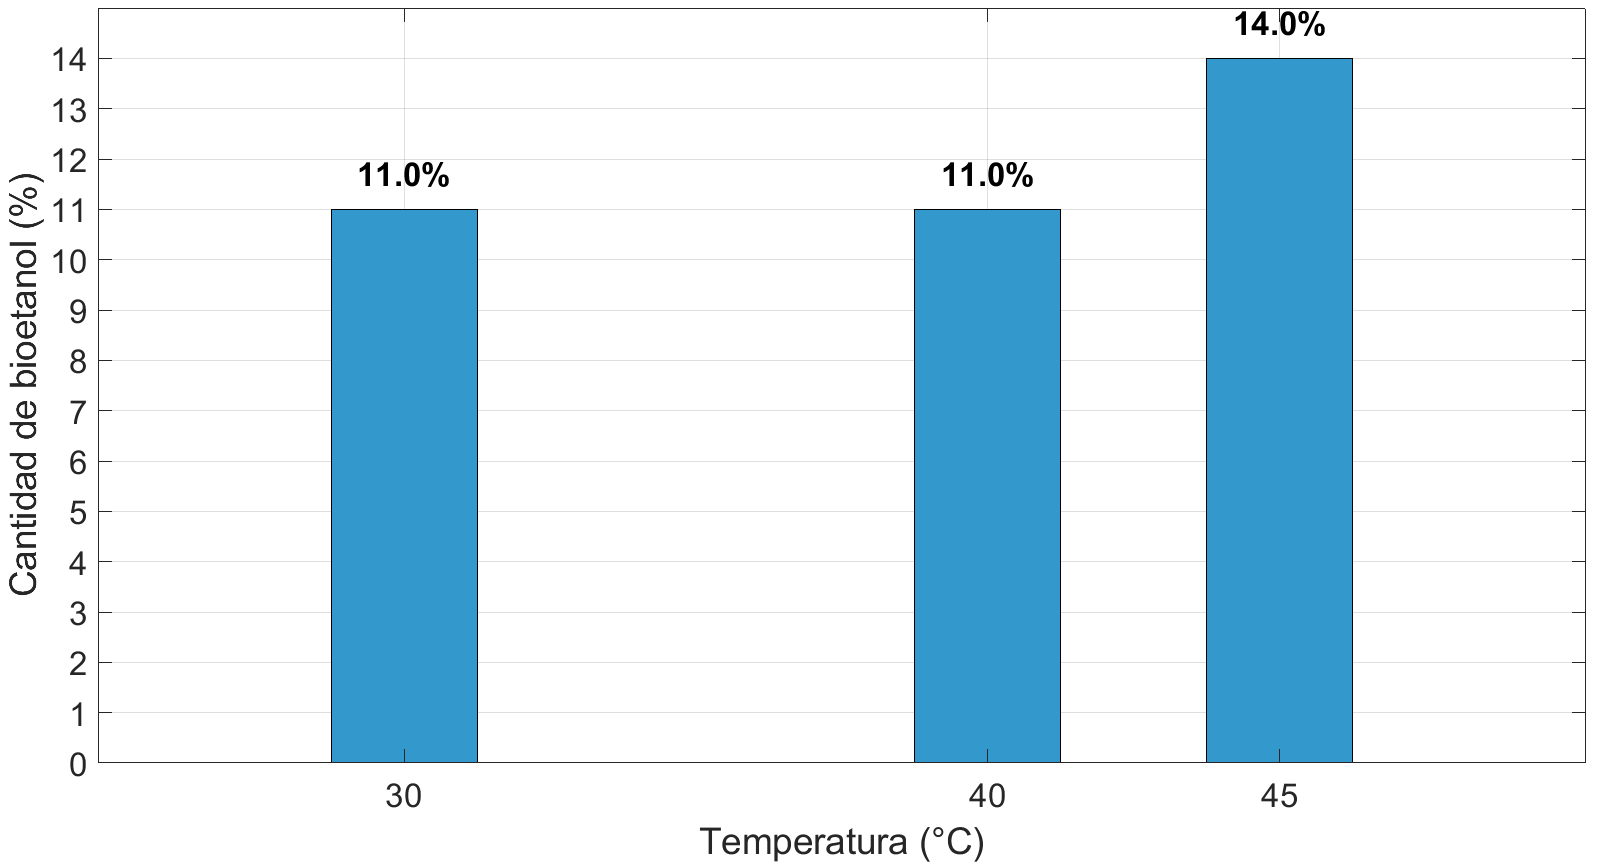
\includegraphics[width=9cm, height=6.2cm]{imagenes/biologico_TNUB}
					\caption{Producción de bioetanol con pretratamiento biológico con bagazo de caña  de TNUB.}
					\label{fig:imagen1}
				\end{subfigure}
				\hfill % Espacio horizontal entre imágenes
				\begin{subfigure}[b]{8 cm}
					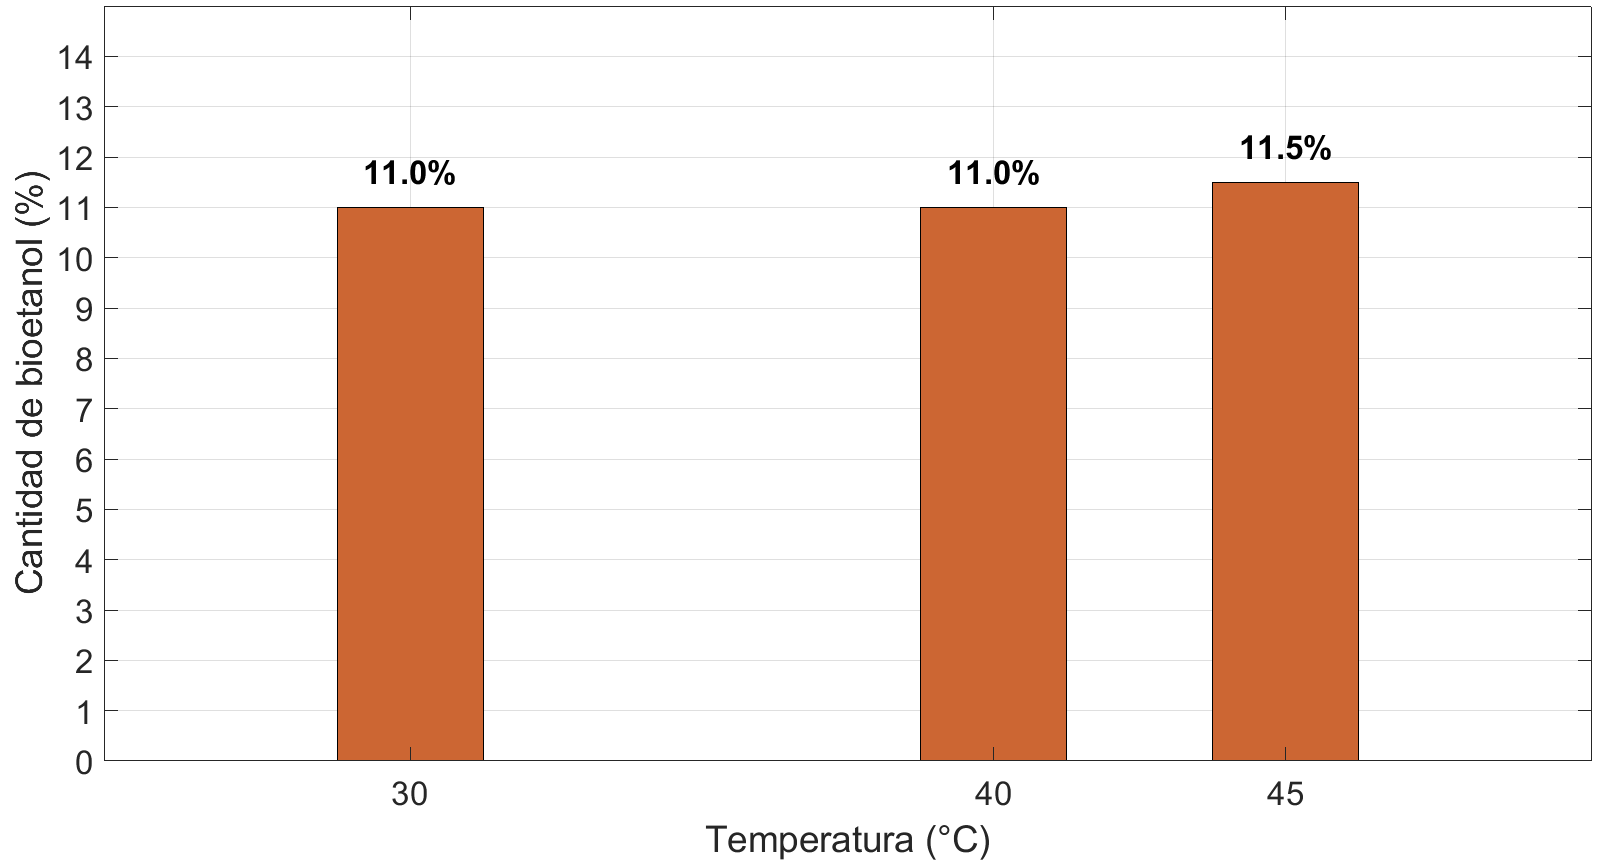
\includegraphics[width=9cm, height=6.2cm]{imagenes/biologico_11}
					\caption{Producción de bioetanol con pretratamiento biológico con bagazo de caña de 1 cm.}
					\label{fig:imagen2}
				\end{subfigure}
				\caption{Producción de bioetanol con pretratamiento biológico.}
				\label{fig:pareja}
			\end{figure}

		
			
			
		
		Para el pretratamiento alcalino se observa que al utilizar TNUB (tamaño no uniforme de biomasa), la variación de temperatura no genera cambios significativos en el proceso. Sin embargo, al emplear un tamaño de partícula de 1 cm, se detectan diferencias notables en el rendimiento, especialmente a una temperatura de 90 °C, donde se registra un impacto significativo en la producción de bioetanol 2G. Para ello podemos ver la Figura \ref{producción}.
			
		
				\begin{figure}[h]
				\centering
				\begin{subfigure}[b]{8 cm}
					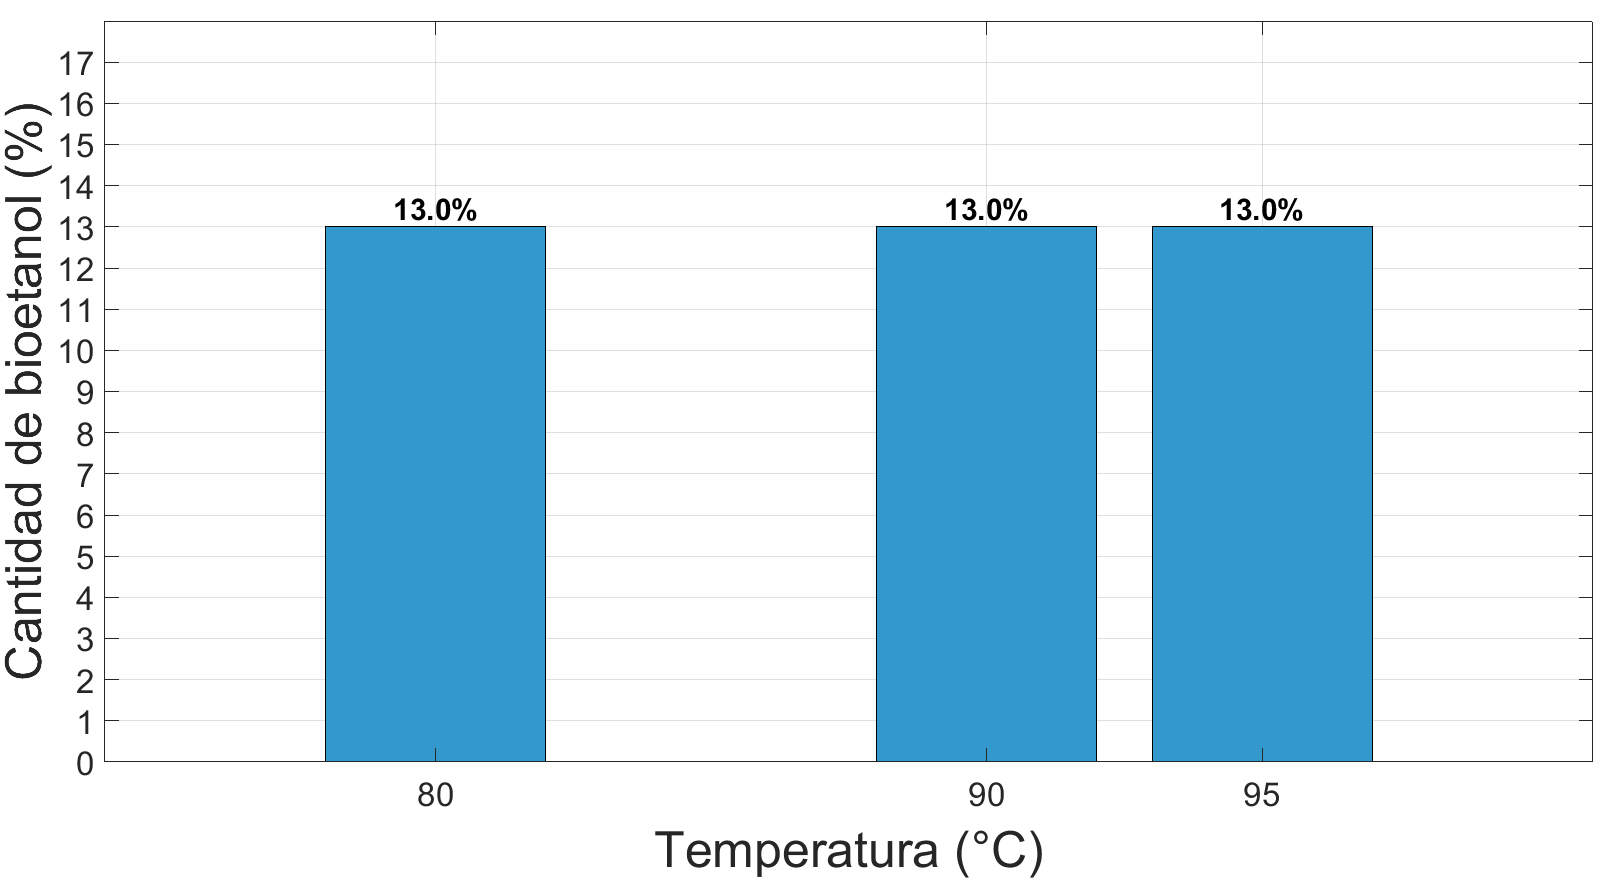
\includegraphics[width=9cm, height=6.2cm]{imagenes/alcalino_TNUB}
					\caption{Producción de bioetanol con pretratamiento alcalino con bagazo de caña  de TNUB.}
					\label{bipoo}
				\end{subfigure}
				\hfill % Espacio horizontal entre imágenes
				\begin{subfigure}[b]{0.49\textwidth}
					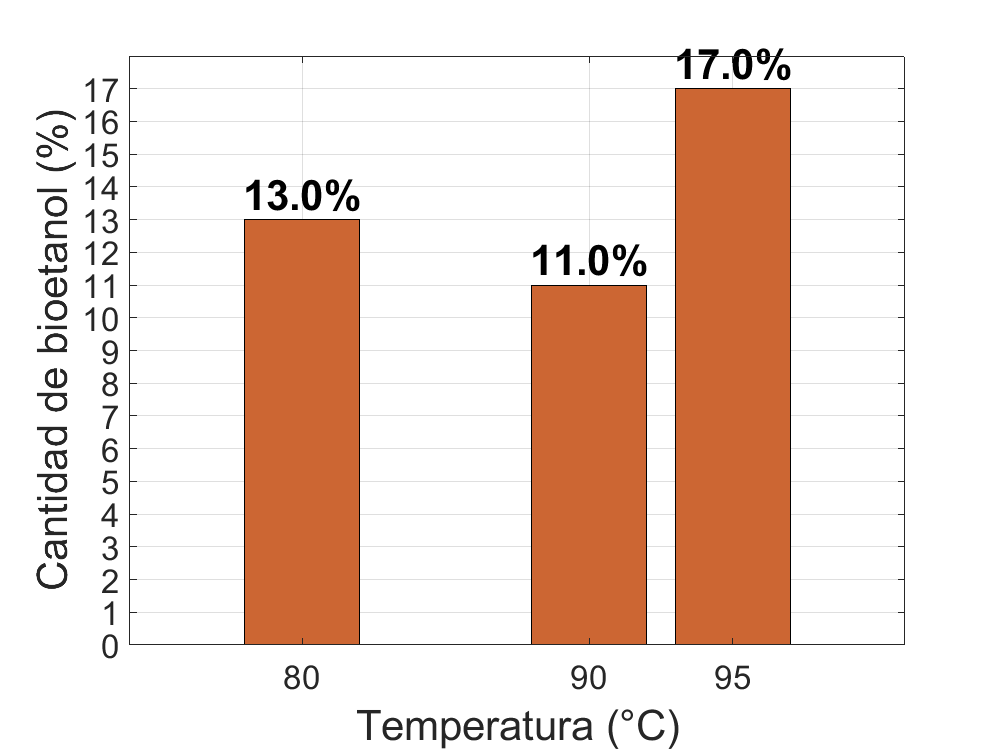
\includegraphics[width=\linewidth]{imagenes/alcalino_1cm}
					\caption{Producción de bioetanol con pretratamiento alcalino con bagazo de caña de 1 cm.}
					\label{fig:imagen11}
				\end{subfigure}
				\caption{Producción de bioetanol con pretratamiento alcalino.}
				\label{producción}
			\end{figure}
			
Para analizar el consumo energético promedio en cada etapa del proceso, la Figura \ref{grafica3} muestra un comparativo detallado entre los dos tipos de pretratamiento evaluados ( pretratamiento biológico,pretratamiento alcalino), además, se incluye a la vez una comparación entre los dos tamaños de partícula estudiados (TNUB y 1 cm).
			
						\begin{figure} [H]
				\centering
				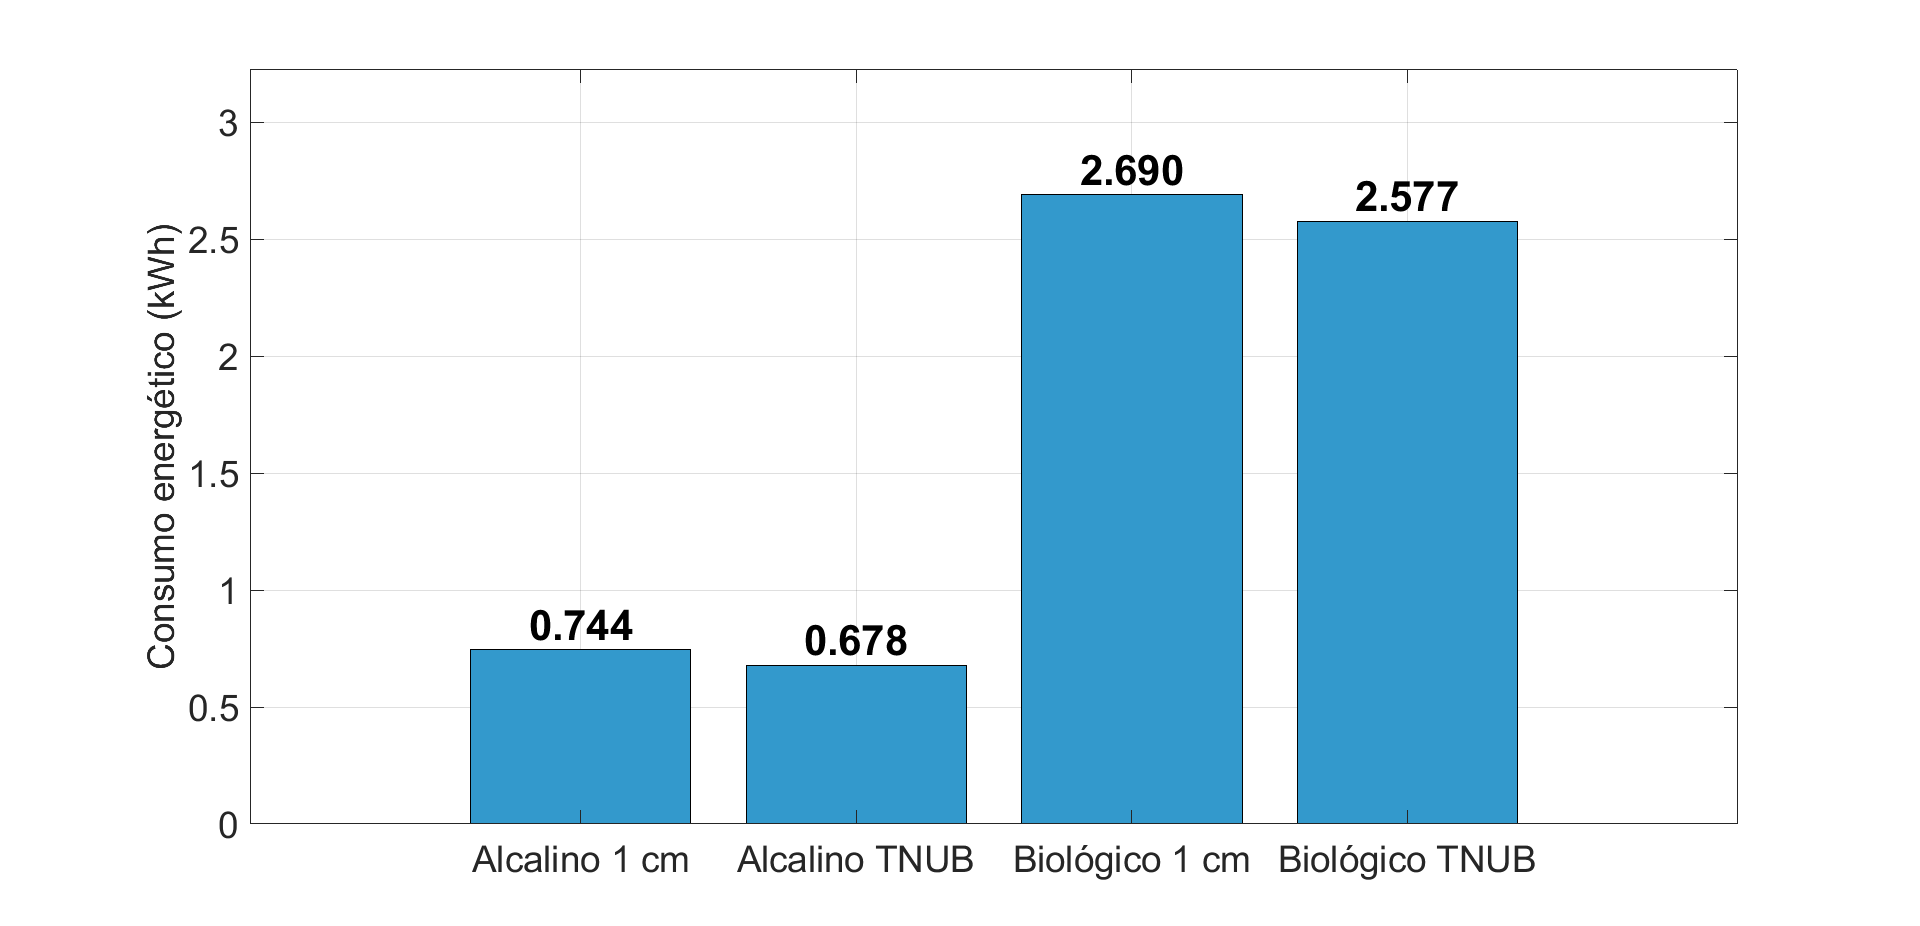
\includegraphics[width=16cm, height=7cm]{imagenes/consumoenergetico}
				\caption{Consumo energético para los dos tipos de pretratamiento. }
				\label{grafica3}
			\end{figure}
			
		Los resultados presentados en la Figura \ref{grafica1} permiten establecer que el pretratamiento biológico demanda un consumo energético 3.7 veces superior al requerido por el pretratamiento alcalino. No obstante, el menor costo unitario por kWh asociado al proceso biológico mitiga sustancialmente su impacto económico global, manteniendo su competitividad como alternativa viable.

\begin{figure} [H]
	\centering
	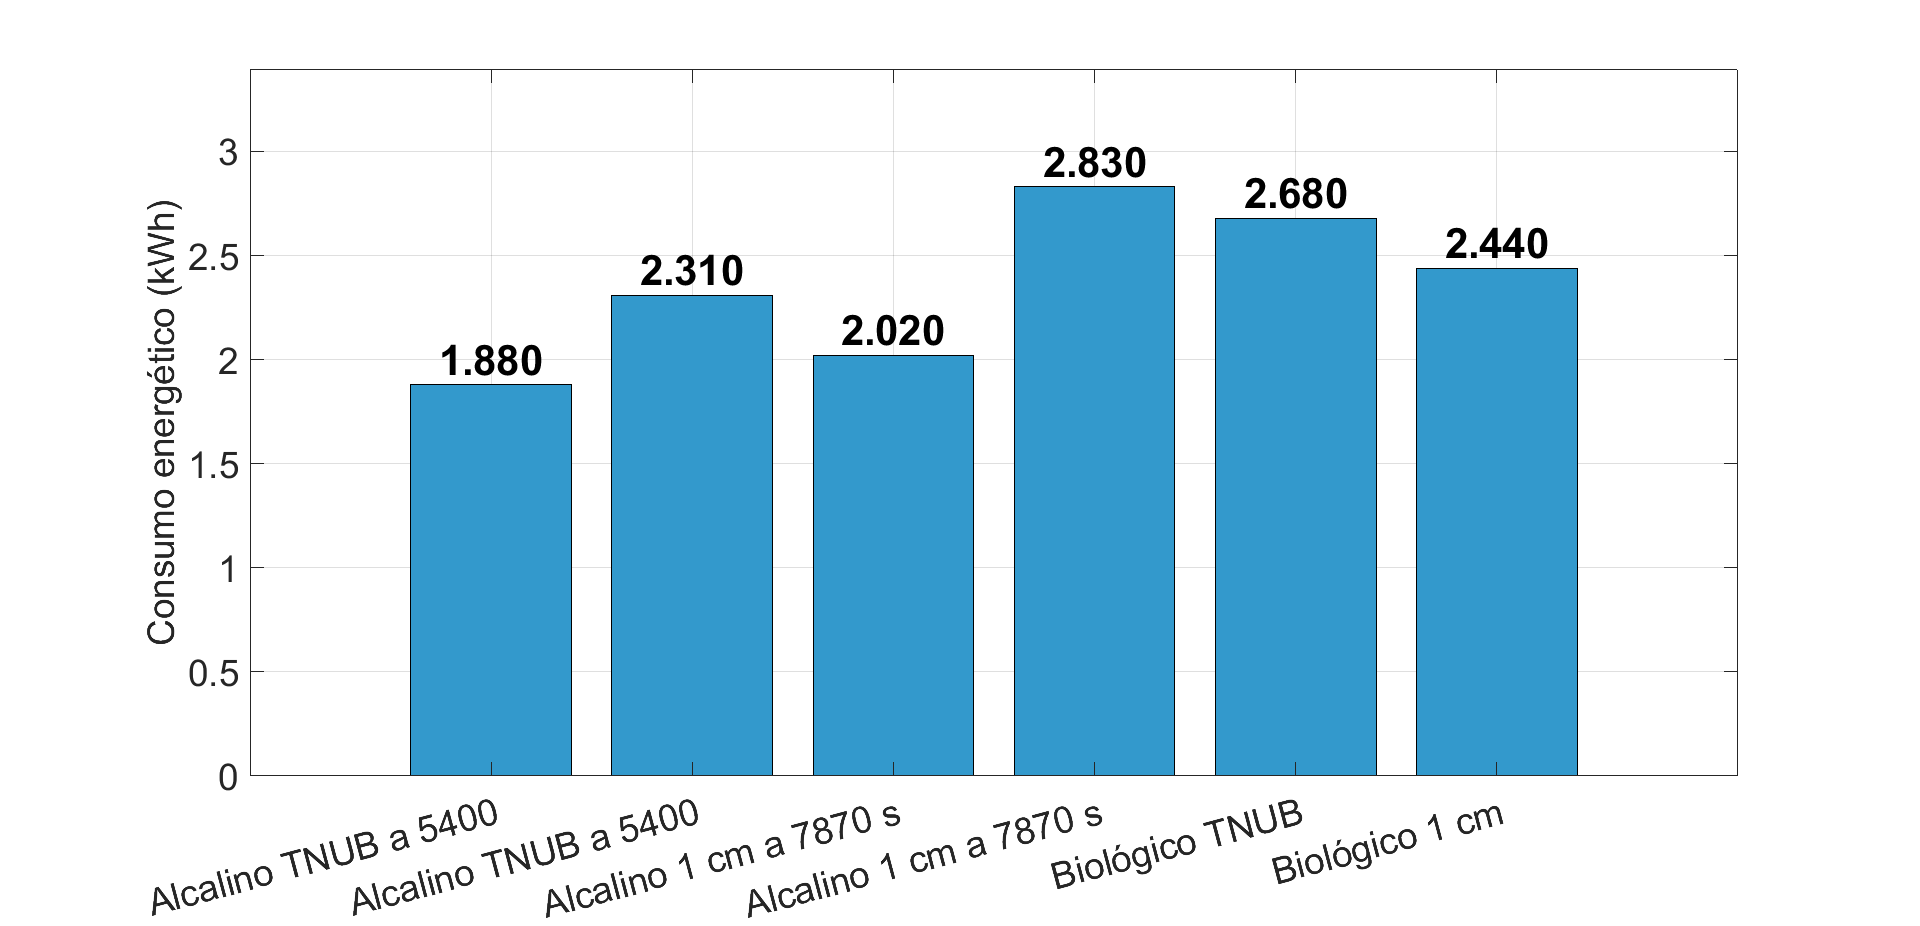
\includegraphics[width=16cm, height=7cm]{imagenes/CONSUMOENERGETICOSSF}
	\caption{Consumo energético para SSF. }
	\label{grafica1}
\end{figure}


Los resultados indican que, durante la SSF, el consumo energético en promedio presentó variaciones mínimas. Este comportamiento podría atribuirse a la influencia del cambio en la temperatura ambiental durante el proceso, ya que las condiciones del lugar posiblemente generan ligeras pérdidas que a su vez implican una demanda ligeramente superior de energía.
En cuanto al costo de producción, en la Figura \ref{grafica} podemos observar el costo total de producción de bioetanol 2G, clasificado por el pretratamiento utilizado, que se obtiene sumando el costo del insumo, el consumo energético promedio y el costo del acondicionamiento del pretratamiento y la SSF.


\begin{figure} [H]
	\centering
	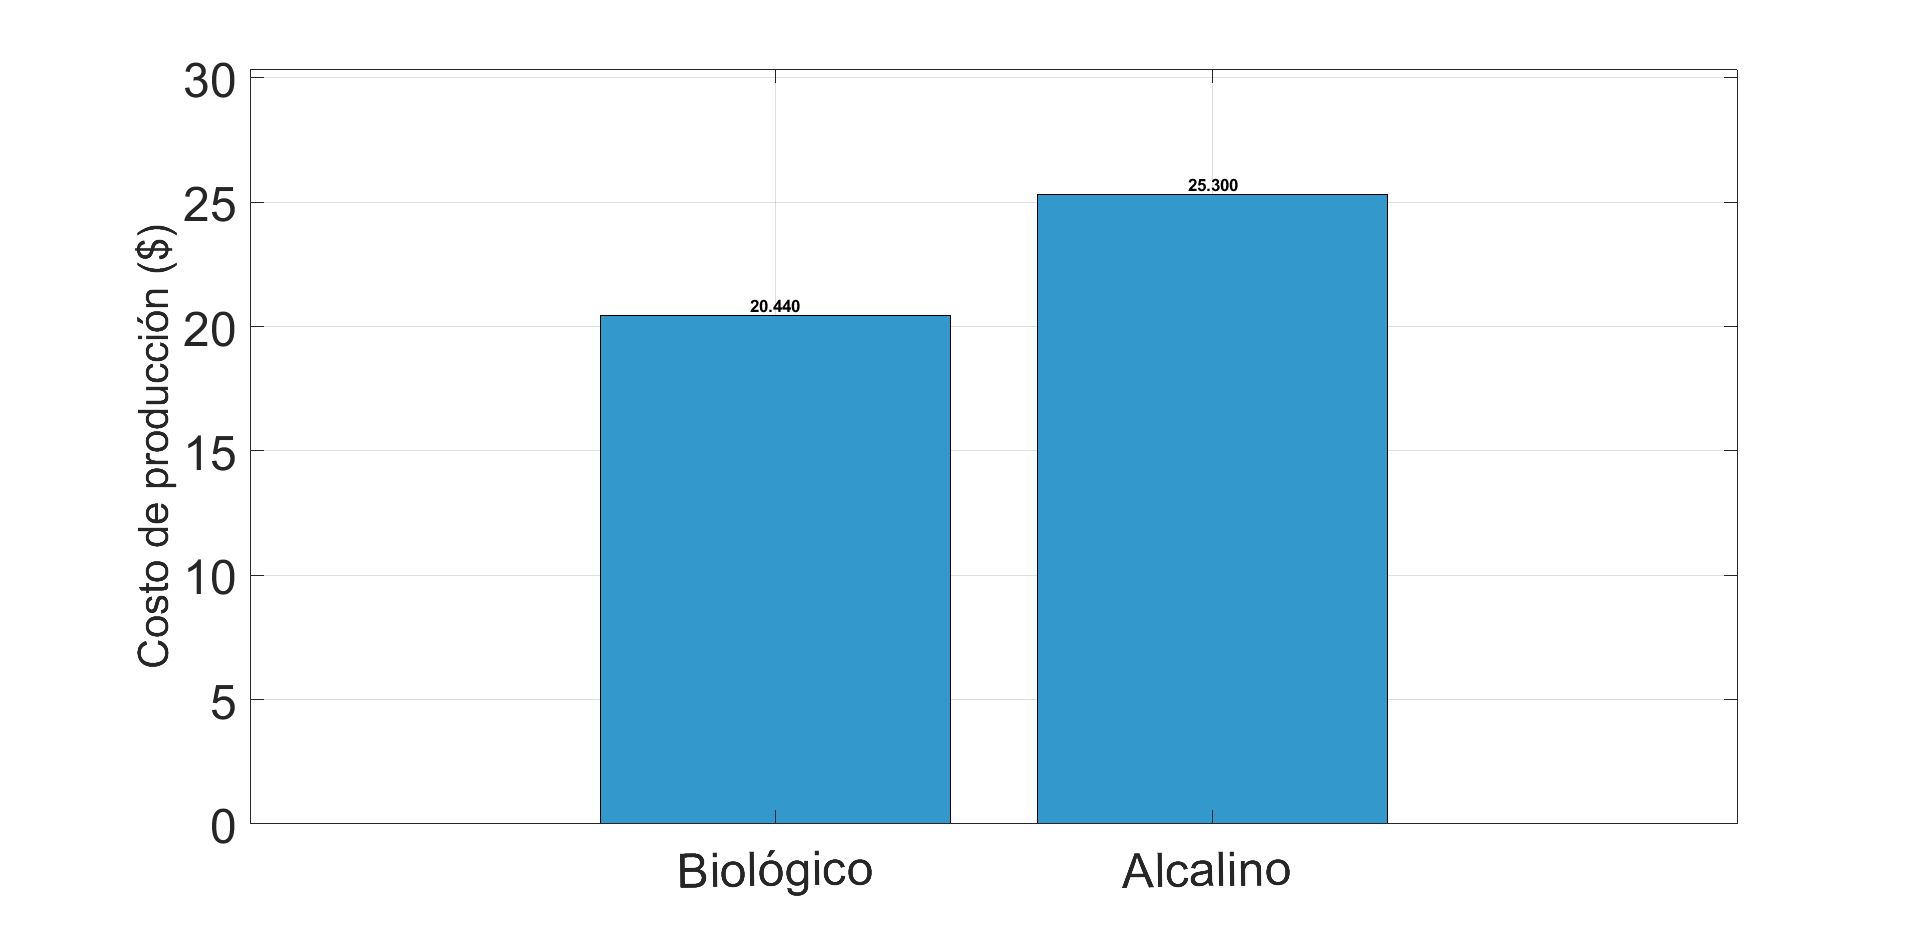
\includegraphics[width=16cm, height=7cm]{imagenes/costos}
	\caption{Consumo energético para SSF. }
	\label{grafica}
\end{figure}
%%%%%%%
\subsubsection{Relación costo producción}
De acuerdo con las observaciones hechas a partir de las tablas antes presentadas, podemos discutir varios aspectos relevantes. En primer lugar, el pretratamiento que produce mayor rendimiento de bioetanol de segunda generación es el alcalino, alcanzando un máximo del 17\% de bioetanol. Sin embargo, al compararlo con el pretratamiento biológico ( cuyo máximo rendimiento fue del 14\% ) encontramos que el costo del pretratamiento alcalino resulta 3.7 veces superior al del tratamiento biológico.

Por lo tanto, el pretratamiento más conveniente desde un punto de vista económico y operativo es el biológico. Aunque presenta un rendimiento ligeramente menor, la diferencia porcentual del contenido de etanol en el producto proveniente de ambos métodos es menor que la diferencia de costo de producción del bioetanol 2G obtenido por estos. Por otro lado, aun quedan por explorar diferentes configuraciones del proceso con tratamiento biológico que pudieran permitir incrementar el contenido de bioetanol en producto. Este es un método que hasta el momento no se ha usado para la producción de bioetanol (ya que originalmente fue propuesto para producir hidrógeno) y aun quedan por analizar más extensamente los efectos de las condiciones de operación.

Respecto a la comparativa de los tamaños de bagazo, los datos muestran que el uso de bagazo de caña de diferentes tamaños genera una menor producción de bioetanol. En consecuencia, la combinación óptima consiste en utilizar un pretratamiento biológico con bagazo de 1 cm, lo que proporciona la mejor relación costo-producción.


%hacer de las tablas el nombre mas grande ................


\newpage
		\section{Conclusión}
		%\begin{itemize}
		Con respecto a lo mencionado anteriormente podemos concluir que en el pretratamiento biológico existe un cambio modificando el tamaño de partícula, así como la temperatura con mayor producción es de 45°.
		Para el pretratamiento alcalino podemos observar que un tiempo de  5400 s no presenta cambios en la producción de bioetanol, aun modificando el tamaño de partícula y la temperatura. En general, se puede concluir que, aunque el pretratamiento con hidróxido de sodio genera una mayor producción promedio de bioetanol en comparación con el humus de lombriz, la diferencia en rendimiento no justifica necesariamente su uso frente al pretratamiento biológico. Este último permite obtener una producción similar con un costo aproximadamente 5 dólares menor, además de presentar una ventaja ambiental clave: no contamina de la misma manera que el hidróxido de sodio, lo que lo convierte en una alternativa más sostenible.
		
		Por otro lado, al evaluar las variables de procesamiento, se observa que el tamaño de partícula de 1 cm en el bagazo es el que proporciona la mayor producción de bioetanol, lo que refuerza la viabilidad del pretratamiento biológico como método eficiente y ecológico para la producción de bioetanol de segunda generación (2G).
		
		En resumen, el pretratamiento con humus de lombriz no solo resulta económicamente favorable, sino también ambientalmente responsable, posicionándose como una opción prometedora para la industria del bioetanol 2G.
		
		
		
		
		
			%\item  Se podría proponer un sistema tolerante a fallas que tome en cuanta la variacion dentro del coeficiente de tranferencia de calor para saber cuando el equipoo se encuentra operando en optimas condiciones y cuando no lo esta haciendo. 
			
		%	\item 
			
		%\end{itemize}
		
		\newpage
\addcontentsline{toc}{section}{7. Bibliografía}:

\bibliographystyle{apalike} 
\bibliography{library}


  		
\section*{Anexos}		
		
\newcounter{anexo}
\setcounter{anexo}{0}

% Para cada anexo:
\stepcounter{anexo}
\anexo{Marco conceptual}

\subsection{ Bioetanol de segunda generación}

	

		\label{marco conceptual}
		
		
	%	\subsection{ Bioetanol de segunda generación}
		
		La producción de bioetanol de segunda generación utiliza como materia prima residuos agrícolas o desechos orgánicos, dependiendo asi de la infraestructura adecuada para obtener la producción de bioetanol. El proceso de producción de bioetanol de segunda generación no tiene una ruta estandarizada, por lo que debe adaptarse a la naturaleza de la materia prima \cite{melendez2022biotecnologia}. El bioetanol de segunda generación se puede obtener con diferentes configuraciones: Sacarificación enzimática de la biomasa pretratada y la fermentación separadas, Sacarificación y fermentación simultáneas, sacarificación y co-fermentación simultáneas y bioproceso consolidado \cite{Gonzalez2018desarrollo}.
		
	\subsection{Definición de conceptos}
		
		
		
		Una parte  importante de la producción de bioetanol de segunda generación es conocer los conceptos, puntualmente los que forman parte del proceso, entre ellos se encuentran el etanol, la biomasa y mas 
		\subsubsection{Etanol}
		El etanol es un tipo de alcohol que en su mayoría es producido a partir de la  fermentación de las azucares fermentables, que se obtienen por microorganismos productores de etanol \cite{GONZALEZ2019Pretratamiento} .Considerado como un combustible ecológico, tipo de alcohol $\text{C}_2\text{H}_5\text{OH}$ (Alcohol etílico), que es obtenido a partir de materia lignocelulosa, puede ser utilizado como sustituto de gasolina por sus propiedades \cite{Ballesteros2002proceso}.
		
		\subsubsection{Biomasa}
	Es un recurso natural, el cual abunda en el planeta, un ejemplo de ello son las plantas, los arboles, el bagazo de caña, entre otros.
		
		\subsubsection{Bagazo de caña}
		El material es recuperado de la producción de azúcar, se obtiene después de un triturado después de obtener el jugo de la caña, este tipo de biomasa no es aprovechada. Esta biomasa tiene un 28\% en peso de la caña, y también, un 45\% de fibra, 2 - 3\% de sólidos insolubles y otro mismo porcentaje de sólidos solubles, finalmente la mitad de este material está conformado de agua \cite{olmo2015bagazo}.
		El bagazo representa el de mayor tonelaje y volumen de la producción de azúcar de caña, generando un promedio de 270 kg de bagazo por tonelada \cite{perez2022efecto}.
		
		\begin{figure}[h]
			\centering
			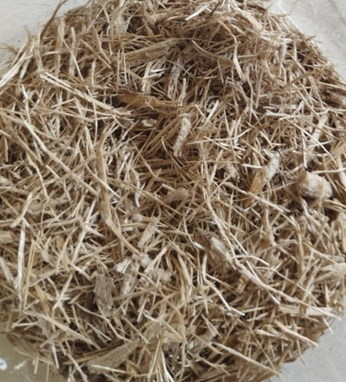
\includegraphics[width=0.4\linewidth]{imagenes/bagazo}
			\caption[Bagazo de caña.]{Bagazo de caña.}
			\label{fig:bagazo}
		\end{figure}
		
		\subsubsection{Lignocelulosa}
		
		Proveniente de la fotosíntesis, la lignocelulosa es uno de los componentes más abundante y principal de la biomasa, esta forma la pared celular de las plantas. Entre las plantas, la composición y porcentajes de lignocelulosa varían, dependiendo de la edad y etapa de crecimiento de las plantas \cite{cuervo2009lignocelulosa}.
		Es viable utilizar este material por su bajo costo, su alta disponibilidad y aprovechamiento variado, un ejemplo es en la industria de los materiales compuestos \cite{jara2022principales}.
		Ya que son viables, se han desarrollado usos alternativos para aprovechar este subproducto agroindustrial, utilizándolo en la creación de biocombustibles.
		La lignocelulosa está conformada por celulosa, hemicelulosa y lignina, siendo una fuente de carbono y energía renovable \cite{portalproduccion}. 
		
		\subsubsection{Pretratamiento}
		
		El pretratamiento es parte importante en el proceso de obtención del bioetanol de segunda generación,dado que el procesamiento de biomasa lignocelulósica complementa la hidrólisis enzimática y posibilita la obtención de altos rendimientos. Siendo necesario ya que la lignina en las paredes celulares en la planta crean barreras contra en ataque enzimático \cite{Riano2010produccion}.
		\newline 
		
		\begin{figure}[H]
			\centering
			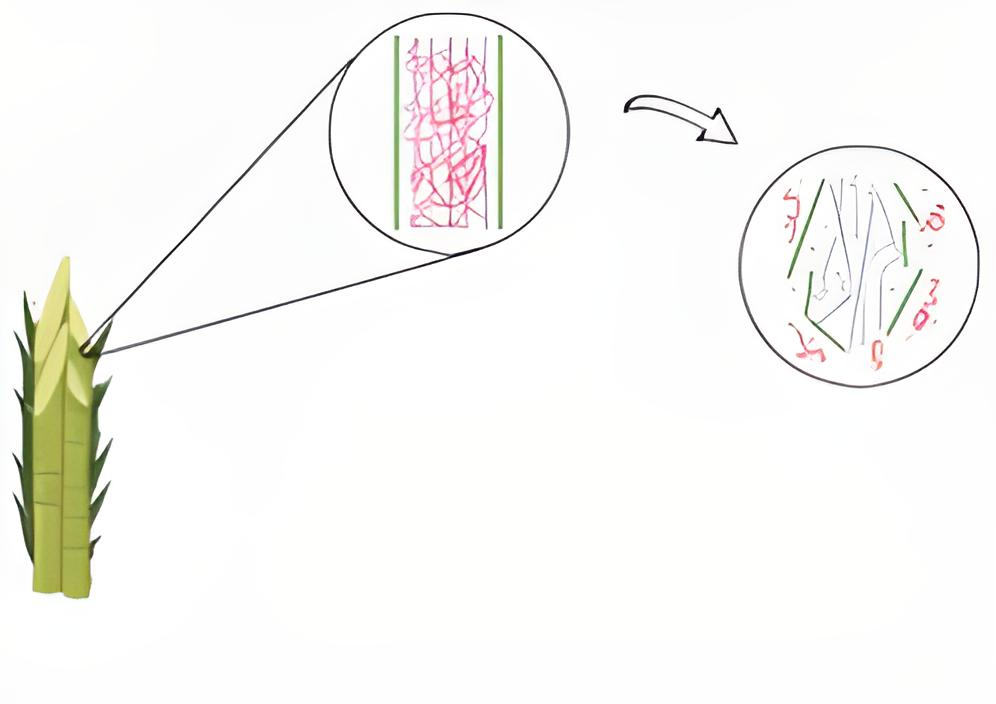
\includegraphics[width=0.4\linewidth]{imagenes/pretrata_1}
			\caption{Efecto del pretratamiento de biomasa ligno-celulósica.}
			\label{fig:pretrata1}
		\end{figure}
		
		
		\subsubsection{Hidrólisis}
		También llamado despolimerización del material lignocelulósico. La biomasa con la dificultad de transformase químicamente  o biológicamente tiene el requisito de realizar una hidrólisis, entre mayor concentración de monosacáridos, mejor sera el rendimiento.La hidrólisis es un proceso que ayuda la formación de azucares siendo muy importante en la producción de etanol y en la obtención de otros productos. Existen distintos tipos de hidrólisis en la Tabla \ref{tipos de hidrolisis} se puede obtener mas información .
		
		\begin{table}[H]
			\centering  
			\caption{Tipos de hidrólisis. }% \citep{ADITIYA2016631} }
			\label{tipos de hidrolisis}
		\begin{tabular}{  | c | c |}
			\hline \textbf{Tipo de hidrólisis} &\textbf{ Proceso y concepto}\\ \hline 
			Hidrólisis ácida   &   Explosión de CO2  \\ 
			
			&   Hidrólisis ácida \\ \hline 
			
			
Térmico			& Expolición de vapor\\
			&  Agua caliente \\ \hline
			Biológico & Bacterias \\
			&  Hongos \\ \hline
			Alcalino  & liquido iónico  \\
			& Hidrólisis alcalina \\ \hline
			Químico   & Ozonólisis\\
			&  Proceso con disolventes orgánicos\\
			& Oxidación húmeda \\ \hline
			Mecánico  & Trituración \\
			&  Pirólisis \\
			&  Microondas \\ \hline
			
		\end{tabular}
		\label{tipos de pretratamientos}
		\end{table}
		
		
		
		\begin{itemize}
		\item  Carga enzimática
		\end{itemize}
		
		Para la hidrólisis enzimática es necesario tomar la carga enzimática a utilizar en la prueba experimental, a carga enzimática se refiere a la cantidad de enzimas utilizadas en el momento de la experimentación, la cantidad de enzima esta dada en UPF (unidades papel filtro),  para obtener el valor en ml se utiliza la formula siguiente, obtenida de \cite{Arturo2022evaluacion}, donde necesitamos los UPF a utilizar y la carga de bagazo pretratado.
		
			\begin{equation}
			 ml = \left( \frac{0.37}{\text{UPF}} \right) \times \textit{cantidad de bagazo} .
			\end{equation}
		
		
		
		\subsubsection{Fermentación}
		La fermentación es un proceso bioquímico complejo, donde los microorganismos metabolizan azúcares y otros componentes para tener como resultado el bioetanol \newline \cite{Escobar2019produccion}, algunos de los microorganismos que pueden transformar son los hongos, bacterias, levaduras. Debido a la complejidad, a que es difícil de controlar y a las múltiples variables que afectan el proceso de fermentación se debe tener un entorno favorable. \cite{rojas2010analisis}
		Es un proceso que se realiza la hidrólisis de los polisacáridos convirtiéndolos en monosacáridos, todo esto en presencia de organismos fermentativos consumiendo los azúcares simples.
		
		
		
		
		\subsection{Configuraciones en la producción de bioetanol}	
		\subsubsection{Sacarificación enzimática de la biomasa pretratada y la fermentación separadas}
		
		El proceso de SHF se realiza por separado debido a que las temperatura que se tienen en las distintas fases son diferentes, en el caso de las enzimas hidrolíticas se tiene un promedio de 50 °C, y una temperatura mas baja en el caso de la fermentación de 30 °C - 32 °C. 
		La producción de biocombustible por etapas separadas es una de las técnicas mas antiguas, realizando un pretratado de enzimas para su hidrólisis y posteriormente una fermentación de la biomasa resultante  \cite{CHOUDHARY201682}.
		
		
		
		
		\subsubsection{Sacarificación y fermentación simultáneas}
		
		En el artículo \cite{CHOUDHARY201682} menciona que la sacarificación se realiza simultáneamente con la fermentación.
		La producción de etanol con microorganismo de importancia industrial como Saccharomyces cerevisiae (levaduras), no permite la utilización completa, este es incapaz de fermentar los azúcares. Se tiene la posibilidad de mantener la concentración de glucosa a un nivel bajo que permite una eficiente co-fermentación.
		%%%%%
		Este se lleva a acabo en un mismo contenedor, solucionando el problema de la utilización de productos para mayor producción de enzimas, siendo un problema limitante en la SHF. Mejorando la eficiencia de la sacarificación enzimática como el rendimiento de etanol. 
		Las enzimas hidrolíticas son adaptables al frío y las levaduras termófilas son importantes que se mantengan a temperatura ambiente \cite{CHOUDHARY201682}.
		
		\subsection{Proceso de obtención de bioetanol 2 G  utilizando una configuración SSF  }		
		Para la producción de bioetanol de segunda generación utilizando una configuración de dos etapas en conjunto, utilizando materia lignocelulósica se utilizan los pasos que menciona el diagrama de la Figura \ref{fig:diagrama-produccionssf}.
	
		\begin{figure}[H]
			\centering
			\includegraphics[width=0.6\linewidth]{imagenes/diagrama producciónssf}
			\caption{Diagrama donde menciona el proceso de bioetanol 2G.}
			\label{fig:diagrama-produccionssf}
		\end{figure}
		
		
	Este diagrama menciona los pasos como el pre-pretratamiento, donde se realiza un clasificado de tamaño de materia lignocelulósico, así como una limpieza y un secado, posteriormente se realiza un pretratamiento donde rompe las barreras de la lignina y obteniendo como resultado una materia con azúcares fermentables. En cuanto a la SSF se toma la materia previamente pretratada a distintas variables.
		
		
		
		\subsection{Pretratamientos}
		En la Tabla \ref{tipos de pretratamientos} se listan los principales pretratamientos, cuya aplicación se reporta en diferentes investigaciones sobre la producción de bioetanol de segunda generación. \cite{ADITIYA2016631} y \cite{Nasution_2022}
		ofrecen dos revisiones completas sobre pretratamientos de biomasa para la producción de bioetanol.
		
		\begin{table}[H]
		\centering  
		\caption{Tipos de pretratamiento. }% \citep{ADITIYA2016631} }
		\begin{tabular}{  | p{5cm} | p{6.5cm} |}
		\hline\textbf{ Tipo de pretratamiento} & \textbf{ Método}\\ \hline 
		Ácido     & Percolación de amoníaco reciclado  \\ 
		&  Ácido diluido  \\
		&  Ácido concentrado \\
		&   Explosión de CO2  \\ 
		&   Hidrólisis ácida \\ \hline 
		Térmico   & Expolición de vapor\\
		&  Agua caliente \\ \hline
		Biológico & Bacterias \\
		&  Hongos \\ \hline
		Alcalino  & liquido iónico  \\
		& Hidrólisis alcalina \\ \hline
		Químico   & Ozonólisis\\
		&  Proceso con disolventes orgánicos\\
		& Oxidación húmeda \\ \hline
		Mecánico  & Trituración \\
		&  Pirólisis \\
		&  Microondas \\ \hline
		
		\end{tabular}
		\label{tipos de pretratamientos}
	\end{table}


\subsubsection{Pretratamiento alcalino}

El pretratamiento con NaOH es uno de los más utilizados en pretratamientos alcalinos,  ya que genera un incremento en la hidrólisis \cite{espinosa2021pretratamiento}, en cambio, producen una perdida de celulosa y hemicelulosa, generando una menor producción de azúcares y bioetanol.
El pretratamiento utiliza, hidróxido sódico, amoniaco o cal, generando menos inhibidores, lo cual obtiene una mayor deslignificación en comparación con tratamiento con ácidos \cite{valles2022estudio}.

\subsubsection{Pretratamiento biológico }

Existen pretratamientos biológicos en los que comúnmente se usan microorganismos, hongos, y enzimas que promueven la degradación de la lignina. El uso de hongos en este tipo de procesos ayuda a descomponer la lignina. En general, estos pretratamientos tienen bajo consumo energético en su implementación, \cite{Gonzalez2018desarrollo}. 




%\subsection{Reactores tipo Batch }





%%%%%%%%%%%%%%%%%%%%%%%%%%%%%%%%%%%%%%%%%%%%%%%%%%%%%%%%%%%%%%%%%%%%%%%%%%%%%%%%%%%%%%%%%%%%%%%%%%%%%%%%%%%%%%%%%%%%%%%%%%%%%%%%%%%%%%%%%%%%%%%%%%%%%%%%%%%%%%%%%%%%%%%%%%%%%%%%%%%%%%%%%%%%%%%%%%%%%%%%%%
	% \newline
	
	
		\anexo{Estado del arte}

	\label{Estado del arte}
El estado del arte es una minuciosa búsqueda de información referente a los avances científicos y tecnológicos de la producción de bioetanol de segunda generación, principalmente utilizando etapas juntas en el proceso. Esta revisión muestra algunos avances en la etapa de pretratamientos en el proceso de producción.

El pretratamiento es un paso muy importante para la producción de bioetanol de segunda generación, algunos de los pretratamientos que existen son: Ácido, Térmico, Biológico, alcalino, Químico, Mecánico \cite{ADITIYA2016631}.
El pretratamiento con NaOH es uno de los más utilizados como pretratamientos alcalinos, este promueve la hidrólisis \newline \cite{espinosa2021pretratamiento}. Una desventaja de este es la pérdida de celulosa y hemicelulosa, y la reducción de azúcares y bioetanol.
En general, el pretratamiento alcalino genera menos inhibidores y favorece la deslignificación, en comparación con tratamiento con ácidos, según \cite{valles2022estudio}. 

También hay pretratamientos biológicos en los que comúnmente se usan microorganismos, hongos, y enzimas que promueven la degradación de la lignina. El uso de hongos en este tipo de procesos ayuda a descomponer la lignina. En general, estos pretratamientos tienen bajo consumo energético en su implementación, \cite{Gonzalez2018desarrollo}.  

%\subsection{Tecnología de bioetanol de segunda generación.}




\subsection{Pretratamientos}



\subsubsection{Pretratamiento Alcalino}

El pretratamiento alcalino consiste en sumergir un material lignocelulósico en una solución alcalina bajo ciertas condiciones de temperatura, concentración, y tiempo de tratamiento. Los álcalis más usados son hidróxido de sodio (NaOH), de potasio (KOH) o de amonio (NH$_4$OH). Estos compuestos rompen los enlaces entre la lignina y los carbohidratos, o solubilizan parcialmente la lignina \cite{Galbe2012}.
% REF. % Galbe, M., & Zacchi, G. (2012). Pretreatment: The key to efficient utilization of lignocellulosic materials. Biomass and Bioenergy, 46, 70?78.
Enseguida se describen algunas investigaciones sobre pretratamientos alcalinos como medio para favorecer la hidrólisis enzimática de la biomasa, que para la actual revisión es el bagazo de caña.

\cite{Nasution_2022} presentó una revisión de los pretratamientos más usados en los últimos años. Como pretratamiento alcalino se destaca el uso del NaOH. Comúnmente se recomienda manejar una concentración al 2 \% de NaOH, una relación de agua destilada de 1:10 solido-liquido, y una temperatura de operación de 80 °C, así como un tiempo de tratamiento de 2h.

En un estudio afin, \cite{Arturo2022evaluacion} utilizó como biomasa bagazo de caña para producir bioetanol con dos modos diferentes de producción: sacarificación enzimática y fermentación en etapas separadas (SHF), y SSF. Se probaron 4 tipos de pretratamientos de la materia prima, entre estos se aplicó un pretratamiento alcalino usando como base NaOH al 2 \% p/v y una carga de bagazo del 4\% p/v. El pretratamiento se llevó a cabo a 97 °C durante un tiempo de 90 minutos. Al finalizar este tiempo, la biomasa tratada se acondicionó mediante etapas de enjuagado, filtrado y secado para después ser procesada por cada modo de producción, SHF o SSF. Comparando el porcentaje de alcohol obtenido a partir de cada proceso (SHF o SSF), se concluyó que el proceso SHF obtuvo un producto más concentrado, con 15 \% de alcohol, mientras que el producto del proceso SSF tenía un contenido de alcohol menor de 11 \%. En contra parte se concluyó que el proceso SSF reduce en un 80\% el tiempo consumido por el proceso SHF.

%\textbf{Conclusión}\\



%\subsubsection{Pretratamiento Biológico}





%%%%%%%%%%%%%%%%%%%%%%%%%%%%%%%%%%%%%%%%%%%%%%%%%%%%%%%%%%%%%%%%%%%%%%%%%%%%%%%%%%%%%%%%%
\subsubsection{Otros pretratamientos} 



\textbf{Pretratamiento ácido} 

El pretratamiento ácido se realiza impregnando en un ácido diluido el material lignocelulósico. Comúnmente se usan ácidos minerales como el ácido sulfúrico (H$_2$SO$_4$), que fragmenta los componentes de la biomasa en moléculas más pequeñas \cite{Galbe2012}. Como ejemplo se citan los siguientes estudios. %%%%%pendiente 
Regresando al trabajo de \cite{Arturo2022evaluacion}, entre los pretratamientos que se presentaron está también uno con H$_2$SO$_4$ y agua destilada. Para este caso se efectuaron experimentos con 3 porcentajes de carga de biomasa (4\%, 6\%, 8\%) a temperatura máxima de 97 °C y con duración de 60 minutos. Para el proceso SSF se obtuvo un producto con 7 \% de alcohol, es decir un rendimiento menor que el obtenido con el pretratamiento alcalino desarrollado en el mismo trabajo para bagazo de caña.

Otro trabajo sobre producción de bioetanol con bagazo de caña  pretratado con ácido es el de \cite{TANTAYOTAI2022102499}, quienes compararon la efectividad de dos ácidos, uno orgánico y otro mineral. Como resultado, se concluyó que el pretratamiento con ácidos orgánicos fue más efectivo porque se logró mayor rendimiento.

%%%%%
\cite{rojas2010analisis} y sus colaboradores también expusieron sus resultados para 3 pretratamientos de bagazo de caña, incluido uno ácido. Su objetivo fue comparar el impacto ambiental de los tres pretratamientos. Al igual que en los trabajos antes citados, el pretratamiento se hizo con H$_2$SO$_4$. Se usó el ácido al 1.5 \% en peso y se procesó a 160 °C. Se obtuvo como resultado la degradación del 90\% de la hemicelulosa y una completa solubilidad de la lignina. Después del pretratamiento se efectuaron la fermentación, la destilación y la purificación del producto. La etapa de SSF se concluyó con un rendimiento de 85 \% de la sacarificación y fermentación de la celulosa, mientras que el rendimiento del proceso SHF fue de 75 \%  con respecto a la fermentación de azucares. Finalmente, se concluyó que al comparar los tres tipos de pretratamientos efectuados, el ácido no se encuentra entre los mas contaminantes.



\textbf{Pretratamiento térmico } 
\newline

Regresando al trabajo de \cite{rojas2010analisis}, otro de los pretratamiento probados para el bagazo de caña fue un pretratamiento térmico en condiciones de temperaturas y presiones elevadas, de 220 °C y 22.9 atm. Al analizar los niveles de contaminación de los pretratamientos, se concluyó que dada la cantidad de energía que se requiere para llegar a altas temperaturas, el pretratamiento térmico resultó el más contaminante.

El trabajo de \cite{MOONSAMY2022115675} tuvo como objetivo lograr una producción autosustentable, creando distintos escenarios. Un aspecto escencial de su análisis fue explorar la vialidad de combinar procesos de primera y segunda generación a partir de melazas y material lignocelulósico provenientes de la caña de azúcar. El pretratamiento propuesto fue el de explosión de vapor. Este consiste en hacer pasar una corriente líquida de hemicelulosa con una parte solida de celulosa y lignina. Posteriormente, dependiendo del escenario se realizó una SSF o una SHF. La conclusión fue que la ventaja del proceso combinado es su factibilidad económica, el reto es evitar la inhibición o supresión de la glucosa.
%%%%%%%%%%%%%%%%%%%%%%%%%%%%%%%%%%%%%%%%%%%%%%%%%%%%%%%%%%%%%%%%%%%%%%%%%%%%%%%%%%%%%%%%%

\subsection{Configuraciones en la producción de bioetanol}



\subsubsection{Sacarificación enzimática de la biomasa pretratada y la fermentación separadas} 

%%% otros
En el artículo de \cite{Gomes2022analisis} se analizaron tres configuraciones para fermentación de bagazo de caña, ante diferentes condiciones de operación en modo por etapas separadas. Con un primer análisis se evaluó la influencia de la humedad, comparando la efectividad del proceso para humedades de la biomasa del 40\% y 60\%. Se concluyó que con menor humedad, el rendimiento de bioetanol aumenta. En un segundo análisis se evaluó el efecto de la velocidad de dilución durante la fermentación. El resultado fue que a mayor velocidad, el producto tiene mayor concentración de etanol. Por último se implementó una SSF, en la que se alcanzó un rendimiento bioetanol/bagazo del 12.5\%. 

%\subsubsection{Sacarificación y fermentación simultáneas} 

%\subsection{Producción de bioetanol de segunda generación en reactores tipo Batch}



		
%	\end{appendix}
	
	
	\anexo{Diseño del control de temperatura}
	
	\label{diseño del control de temp}
	
	
	
	\subsection{Respuesta de la planta aplicando una Señal PRBS}
	
	
	La señal PRBS entra  mediante la salida PWM del arduino a un convertidor, pasando después a la resistencia como se muestra en el diagrama de la Figura \ref{ diagrama_prbs}.
	
	\begin{figure}[H]
		\centering
		\includegraphics[width=.4\linewidth]{imagenes/diagrama_PRBS}
		\caption{Señal PRBS. }
		\label{ diagrama_prbs}
	\end{figure}
	
	En el reactor se mide mediante los sensores termopar k  la temperatura, esta temperatura ingresando la señal PWM tiene la forma siguiente como lo muestra la Figura \ref{ Temperatura_con PRBS}.
	
	\begin{figure}[H]
		\centering
		\includegraphics[width=.8\linewidth]{imagenes/temperatura con prbs}
		\caption{Comportamiento de la temperatura dentro del reactor con señal de entrada . }
		\label{ Temperatura_con PRBS}
	\end{figure}
	
	
	Como se puede observar en la imagen la temperatura sufre de variaciones,  sin embargo, dichas variaciones ayudaran a obtener la identificación del sistema con mayor precisión de la planta.
	Para obtener la temperatura neta del sistema , es decir la temperatura sin la influencia de la temperatura ambiente se resta la temperatura ambiente dentro del laboratorio menos la temperatura dentro del biorreactor.	La gráfica de la Figura \ref{ Temperatura neta_con PRBS} muestrala temperatura dentro del reactor cuando llega a la referencia.
	
	\begin{figure}[H]
		\centering
		\includegraphics[width=.7\linewidth]{imagenes/temp_neta}
		\caption{Comportamiento de la temperatura sin la temperatura ambiente dentro del laboratorio. }
		\label{ Temperatura neta_con PRBS}
	\end{figure}
	
	La gráfica de la Figura \ref{ Temperatura neta_con PRBS} muestrala temperatura dentro del reactor.
	
	
	
	\subsection{Identificación del sistema de la planta}	
	
	Se necesita un sistema que modele el comportamiento de la temperatura de la planta, por lo que se realizaron técnicas de identificación, como es el caso de la técnica OE donde se obtiene el sistema.
	
	
	\begin{equation}
		G(s) = \frac{0.0005369 \, s^2 + 0.0003022 \, s + 8.207 \times 10^{-5}}{s^3 + 0.3314 \, s^2 + 0.0002728 \, s + 2.707 \times 10^{-7}}
	\end{equation}
	
	Esta función de transferencia tiene respuesta como se muestra en la siguiente figura \ref{fig:identificacion}, este sistema es de tercer orden.
	
	
	\begin{figure} [H]
		\centering
		\includegraphics[width=0.8\linewidth]{imagenes/identificacion}
		\caption{Comportamiento del sistema.}
		\label{fig:identificacion}
	\end{figure}
	Para observar el comportamiento del sistema se puede ver los polos y ceros del sistema en la figura \ref{polos y ceros}.
	
	\begin{figure} [h]
		\centering
		\includegraphics[width=1\linewidth]{imagenes/Polos y ceros}
		\caption{Polos y ceros del sistema.}
		\label{polos y ceros}
	\end{figure}
	\newpage
	%%%%%%%%%%%%%%%%%%%%%%%%%%%%%%%%%%%%%%%%%%%%%%%%%%%%%%%%%%%%

	\subsection{Control PID}
	
	
	
	Un control PID puede ser calculado con la siguiente ecuación 
	
	\begin{equation}
		C(t) = K_p \, e(t) + K_i \int e(t) \, dt + K_d \frac{d e(t)}{dt}.
	\end{equation}
	Para el control PID se utilizo la herramienta de MATLAB que tiene por nombre PID TUNER (Transfer function Based).
	
	\begin{figure}[h!]
		\centering
		\includegraphics[width=0.7\linewidth]{imagenes/pid tuner}
		\caption{Ventana de la herramienta PID Tuner}
		\label{fig:pid-tuner}
	\end{figure}
	
	Obteniendo como resultado los valores de cada variable del controldador PID:
	\begin{equation}
		P=0.00724555643948787 .
	\end{equation}
	
	\begin{equation}
		I=9.60342545392904 X 10^{-07}.
	\end{equation}
	
	\begin{equation}
		D=5.63241452981354.
	\end{equation}
	
	Realizando un ajuste a los valores de la planta obteniendo como nuevos valores lo siguiente:
	
	\begin{equation}
		P=0.19779.
	\end{equation}
	
	\begin{equation}
		I=2.835 X 10^{-04}.
	\end{equation}
	
	\begin{equation}
		D=-1.72.
	\end{equation}
	
	Con estos valores se observa el control en las variables en el reactor, utilizando la herramienta MATLAB como lo muestra la figura \ref{sistema simulado}.
	
	\begin{figure}[H]
		\centering
		\includegraphics[width=0.8\linewidth]{imagenes/sistema_controlado}
		\caption{Sistema simulado con control a 90 °C.}
		\label{sistema simulado}
	\end{figure}
	
  En cada paso de la producción de bietanol se realizaron diseños de control para la temperatura, por lo que en la Tabla \ref{tabla_control} se presentan los valores para cada parte de control.
	 
	
	
	\begin{table}[H]
		\centering
		\caption{Valores para el control de temperatura en pretratamiento y SSF.}
		\begin{tabular}{|l|l|l|l|}
			\hline
			Variables & Pretratamiento Bilógico & Pretratamiento alcalino & SSF \\ \hline
			P & 0.5 & 0.19779 & 0.197 \\ \hline
	    	I & $2 x10^-9 $ & $2.835 x10^-4 $ & $2.8 x10^-8 $ \\ \hline
			D & 1.6 & -1.72 & -1.7 \\ \hline
\end{tabular}
\label{tabla_control}
\end{table}
	
	
	
	
	
	\end{document}